\clearpage
%&latex
\documentclass[a4paper]{article}

\frenchspacing

\usepackage[cp1250]{inputenc}
\usepackage{czech}

\usepackage{a4wide}
\usepackage{amsmath, amsthm, amssymb, amsfonts}
\usepackage[mathcal]{eucal}




\font\bigrm = csr10 scaled \magstep 2
\font\bigbf = csb10 scaled \magstep 4

%Vacsina prostredi je dvojjazicne. V pripade, ze znenie napr pozorovania je pisane po slovensky, malo by byt po slovensky aj oznacenie.

\newenvironment{pozadavky}{\pagebreak[2]\noindent\textbf{Po�adavky}\par\noindent\leftskip 10pt}{\par\bigskip}
\newenvironment{poziadavky}{\pagebreak[2]\noindent\textbf{Po�iadavky}\par\noindent\leftskip 10pt}{\par\bigskip}

\newenvironment{definice}{\pagebreak[2]\noindent\textbf{Definice}\par\noindent\leftskip 10pt}{\par\bigskip}
\newenvironment{definiceN}[1]{\pagebreak[2]\noindent\textbf{Definice~}\emph{(#1)}\par\noindent\leftskip 10pt}{\par\bigskip}
\newenvironment{definicia}{\pagebreak[2]\noindent\textbf{Defin�cia}\par \noindent\leftskip 10pt}{\par\bigskip}
\newenvironment{definiciaN}[1]{\pagebreak[2]\noindent\textbf{Defin�cia~}\emph{(#1)}\par\noindent\leftskip 10pt}{\par\bigskip}

\newenvironment{pozorovani}{\pagebreak[2]\noindent\textbf{Pozorov�n�}\par\noindent\leftskip 10pt}{\par\bigskip}
\newenvironment{pozorovanie}{\pagebreak[2]\noindent\textbf{Pozorovanie}\par\noindent\leftskip 10pt}{\par\bigskip}
\newenvironment{poznamka}{\pagebreak[2]\noindent\textbf{Pozn�mka}\par\noindent\leftskip 10pt}{\par\bigskip}
\newenvironment{poznamkaN}[1]{\pagebreak[2]\noindent\textbf{Pozn�mka~}\emph{(#1)}\par\noindent\leftskip 10pt}{\par\bigskip}
\newenvironment{lemma}{\pagebreak[2]\noindent\textbf{Lemma}\par\noindent\leftskip 10pt}{\par\bigskip}
\newenvironment{lemmaN}[1]{\pagebreak[2]\noindent\textbf{Lemma~}\emph{(#1)}\par\noindent\leftskip 10pt}{\par\bigskip}
\newenvironment{veta}{\pagebreak[2]\noindent\textbf{V�ta}\par\noindent\leftskip 10pt}{\par\bigskip}
\newenvironment{vetaN}[1]{\pagebreak[2]\noindent\textbf{V�ta~}\emph{(#1)}\par\noindent\leftskip 10pt}{\par\bigskip}
\newenvironment{vetaSK}{\pagebreak[2]\noindent\textbf{Veta}\par\noindent\leftskip 10pt}{\par\bigskip}
\newenvironment{vetaSKN}[1]{\pagebreak[2]\noindent\textbf{Veta~}\emph{(#1)}\par\noindent\leftskip 10pt}{\par\bigskip}

\newenvironment{dusledek}{\pagebreak[2]\noindent\textbf{D�sledek}\par\noindent\leftskip 10pt}{\par\bigskip}
\newenvironment{dosledok}{\pagebreak[2]\noindent\textbf{D�sledok}\par\noindent\leftskip 10pt}{\par\bigskip}

\newenvironment{dokaz}{\pagebreak[2]\noindent\leftskip 10pt\textbf{D�kaz}\par\noindent\leftskip 10pt}{\par\bigskip}
\newenvironment{dukaz}{\pagebreak[2]\noindent\leftskip 10pt\textbf{D�kaz}\par\noindent\leftskip 10pt}{\par\bigskip}

\newenvironment{priklad}{\pagebreak[2]\noindent\textbf{P��klad}\par\noindent\leftskip 10pt}{\par\bigskip}
\newenvironment{prikladSK}{\pagebreak[2]\noindent\textbf{Pr�klad}\par\noindent\leftskip 10pt}{\par\bigskip}
\newenvironment{priklady}{\pagebreak[2]\noindent\textbf{P��klady}\par\noindent\leftskip 10pt}{\par\bigskip}
\newenvironment{prikladySK}{\pagebreak[2]\noindent\textbf{Pr�klady}\par\noindent\leftskip 10pt}{\par\bigskip}

\newenvironment{algoritmusN}[1]{\pagebreak[2]\noindent\textbf{Algoritmus~}\emph{(#1)}\par\noindent\leftskip 10pt}{\par\bigskip}
%obecne prostredie, ktore ma vyuzitie pri specialnych odstavcoch ako (uloha, algoritmus...) aby nevzniklo dalsich x prostredi
\newenvironment{obecne}[1]{\pagebreak[2]\noindent\textbf{#1}\par\noindent\leftskip 10pt}{\par\bigskip}


\newenvironment{penumerate}{
\begin{enumerate}
  \setlength{\itemsep}{1pt}
  \setlength{\parskip}{0pt}
  \setlength{\parsep}{0pt}
  %\setlength{\topsep}{200pt}
  \setlength{\partopsep}{200pt}
}{\end{enumerate}}

\def\pismenka{\numberedlistdepth=2} %pouzit, ked clovek chce opismenkovany zoznam...

\newenvironment{pitemize}{
\begin{itemize}
  \setlength{\itemsep}{1pt}
  \setlength{\parskip}{0pt}
  \setlength{\parsep}{0pt}
}{\end{itemize}}

\definecolor{gris}{gray}{0.95}
\newcommand{\ramcek}[2]{\begin{center}\fcolorbox{white}{gris}{\parbox{#1}{#2}}\end{center}\par}

\clearpage

\title{\LARGE U�ebn� texty k st�tn� bakal��sk� zkou�ce \\ Matematika}


\begin{document}

\maketitle

\vspace{10mm}
\begin{center}
\includegraphics[scale=0.5]{../common/logo.pdf}
\end{center}
\vfill
\begin{center}
\Large podle po�adavk� od roku 2008
\end{center}
\vfill

\clearpage
\emph{V�en� �tudent/�itate�},

toto je zbierka vypracovan�ch ot�zok pre bakal�rske sk��ky Informatikov. Ot�z\-ky boli vypracovan� �tudentmi MFF po�as pr�pravy na tieto sk��ky, a teda zatia� neboli overen� kvalifikovan�mi osobami (profesormi/dokotorandmi mff at�.) - preto nie je �iadna z�ruka ich spr�vnosti alebo �plnosti.

V��ina textov je vypracovan� v �estine resp. sloven�ine, pros�me dodr�ujte t�to konvenciu (a obmedzujte teda pou��vanie napr. anglick�ch textov). Ak n�jdete nejak� chybu, nepresnos� alebo ne�pln� inform�ciu - nev�hajte kontaktova� administr�tora alebo niektor�ho z prispievate�ov, ktor� m� write-pr�stup k svn stromu, s opravou :-) Podobne - ak n�jdete v \uv{texte} veci ako ??? a TODO, znamen� to �e dan� inform�ciu je potrebn� skontrolova�, resp. doplni�...

Texty je mo�n� �alej pou��va� a ��ri� pod licenciou \textbf{GNU GFDL} (�o pre v�etk�ch prispievaj�cich znamen�, �e musia s�hlasi� so zverejnen�m svojich �prav pod�a tejto licencie).

Ver�me, �e V�m tieto texty pom��u k �spe�n�mu zlo�eniu sk��ok.

\begin{center}
\line(1,0){300}
\end{center}

\textbf{Hlavn� write�i :-) }:
\begin{pitemize}
	\item \emph{ajs}
	\item \emph{andree} -- http://andree.matfyz.cz/
	\item \emph{Hydrant}
	\item \emph{joshis / Petr Dvo��k}
	\item \emph{kostej}
	\item \emph{nohis}
	\item \emph{tuetschek} -- http://tuetschek.wz.cz/
\end{pitemize}

�vodn� verzie niektor�ch textov vznikli prepisom ot�zok vypracovan�ch \uv{p�somne na papier}, alebo inak ne-{\TeX}-ovsky. Autormi t�chto p�vodn�ch verzi� s� najm� nasleduj�ce osoby:
\emph{gASK}, \emph{Grafi}, \emph{Kate} (mat-15), \emph{Nytram}, \emph{Oscar}, \emph{Stando}, \emph{xStyler}. �as� je prebrat� aj z p�vodn�ch s�borkov�ch textov...
V�etk�m patr� na�a/va�a v�aka.

V roce 2011 n�kter� ot�zky updatovali a roz���ili: Karel B�lek (\url{http://karelbilek.com}), Petr �e�il, Michal Krkavec.
\clearpage

\tableofcontents


\newpage
\section{��sla}

\begin{pozadavky}
\begin{pitemize}
\item Vlastnosti p�irozen�ch, cel�ch, racion�ln�ch, re�ln�ch a komplexn�ch ��sel
\item Posloupnosti a limity
\item Cauchyovsk� posloupnosti
\end{pitemize}
\end{pozadavky}

\subsection{Re�ln� ��sla}
Jedna mo�nost je definovat $\mathbb{R}$ axiomaticky.

\begin{definice}
Mno�inou v�ech re�ln�ch ��sel (zna��me ji $\mathbb{R}$) budeme rozum�t mno�inu, na n� je definov�no s��t�n� (zna��me $x+y$), n�soben� (zna��me $x\cdot y$) a uspo��d�n� (zna��me $x \le y$), kter� sp�uj� tyto axiomy:

\begin{penumerate}
	\item (Algebraick� operace)
	\begin{penumerate}
		\item $\forall x,y,z \in \mathbb{R} : x+(y+z) = (x+y)+z \hfill\textit{(asociativn� z�kon pro s��t�n�)}$
		\item $\forall x,y \in \mathbb{R} : x+y = y+x \hfill\textit{(komutativn� z�kon pro s��t�n�)}$
		\item v $\mathbb{R}$ existuje nulov� prvek (zna��me ho 0) tak, �e $\forall x \in \mathbb{R}: x+0 = x$
		\item pro ka�d� $x \in \mathbb{R}$ existuje opa�n� prvek (zna��me ho $-x$) tak, �e $x+(-x)=0$
		\item $\forall x,y,z \in \mathbb{R}: x\cdot (y\cdot z)=(x\cdot y)\cdot z \hfill\textit{(asociativn� z�kon pro n�soben�)}$
		\item $\forall x,y \in \mathbb{R} : x\cdot y = y\cdot x \hfill\textit{(komutativn� z�kon pro n�soben�)}$
		\item v $\mathbb{R}$ existuje jednotkov� prvek (zna��me ho 1) tak, �e $\forall x \in \mathbb{R}: x\cdot 1=x$
		\item pro ka�d� $x \in \mathbb{R}, x \neq 0$ existuje inverzn� prvek (zna��me ho $x^{-1}$) tak, �e $x\cdot x^{-1}=1$
		\item $\forall x,y,z \in \mathbb{R}: (x+y)\cdot z = x\cdot z + y\cdot z \hfill\textit{(distributivn� z�kon)}$
	\end{penumerate}
	\item (Uspo��d�n�)
	\begin{penumerate}
		\item $\forall x,y,z \in \mathbb{R}: ((x \le y) \wedge (y \le z)) \Rightarrow (x \le z) \hfill\textit{(tranzitivita)}$
		\item $\forall x,y \in \mathbb{R}: (((x \le y) \wedge (y \le x)) \Rightarrow (x=y) \hfill\textit{(slab� antisymetrie)}$
		\item $\forall x,y \in \mathbb{R}: (x \le y) \vee (y \le x)$
		\item $\forall x,y,z \in \mathbb{R}: (x \le y) \Rightarrow (x+z \le y+z)$
		\item $\forall x,y,z \in \mathbb{R}: (x \le y) \wedge (0 \le z) \Rightarrow (x\cdot z \le y\cdot z)$
	\end{penumerate}
	\item (Netrivialita)
	\begin{penumerate}
		\item $0 \neq 1$
	\end{penumerate}
	\item (�plnost)
		\\\begin{definiceN}{Axiom suprema}
		Nech� $M \subset \mathbb{R}$ je nepr�zdn� a shora omezen�. Pak existuje ��slo $s \in \mathbb{R}$, kter� m� vlastnosti:
		\begin{penumerate}
			\item $\forall x \in M: x \le s$
			\item $\forall s' \in \mathbb{R}, s' < s\;\; \exists x \in M: x > s'$
		\end{penumerate}
		
		\end{definiceN}
\end{penumerate}

\end{definice}
\begin{poznamka}
Axiom supr�ma je d�le�it�, odli�uje re�ln� ��sla od racion�ln�ch.


		��slo $s$ z axiomu suprema je jednozna�n� ur�eno, zna�� se $\sup M$ a ��k� se mu \emph{supremum mno�iny $M$}. Supremum mno�iny je jej� nejmen�� horn� z�vora (\emph{horn� z�vora} je ka�d� takov� prvek, pro kter� plat� bod (a) definice suprema). Nejv�t�� doln� z�voru mno�iny $M$ (pokud existuje --- a d� se dok�zat, �e existuje, je-li mno�ina zdola omezen�) naz�v�me \emph{infimem mno�iny $M$} a zna��me $\inf M$.
\end{poznamka}

\begin{poznamka}
Relace \uv{$<$} na re�ln�ch ��slech (a stejn� tak na p�irozen�ch a racion�ln�ch ��slech) se definuje takto: $a<b$, pr�v� kdy� $a\leq b$ a z�rove� $a\neq b$.
\end{poznamka}

V tomto p��stupu, ve kter�m budu v dal��ch kapitol�ch pokra�ovat, jsme si axiomaticky vytvo�ili $\mathbb{R}$; $\mathbb{N}$ a $\mathbb{Q}$ budu definovat v dal��ch kapitol�ch jako jejich podmno�iny. 

$\mathbb{R}$ lze ale definovat i \uv{obr�cen�}, pokud u� m�me definovanou mno�inu $\mathbb{Q}$ a na n� u� m�me zadefinov�nu limitu a Cauchyovsk� posloupnosti. Lze dok�zat, �e tyto definice jsou ekvivalentn�.

\begin{definice}
Nech� $R$ je mno�ina v�ech Cauchyovsk�ch posloupnost� ve $\mathbb{Q}$. Operace na t�to mno�in� definujeme n�sledovn�:
\begin{itemize}
	\item $\left\{x_n\right\} + \left\{y_n\right\} = \left\{x_n + y_n\right\}$
	\item $\left\{x_n\right\} \cdot \left\{y_n\right\} = \left\{x_n \cdot y_n\right\}$
	\item $\left\{x_n\right\} \ge \left\{y_n\right\}$, pr�v� kdy� $\exists n_0\;\; \forall n>n_0: x_n\ge y_n$
\end{itemize}
Na $R$ definujme relaci ekvivalence jako $\left\{x_n\right\} \sim \left\{y_n\right\}  \Leftrightarrow \lim_{k\rightarrow \infty}\left|x_k-y_k\right|=0$ (je nutn� je�t� dok�zat, �e jde o ekvivalenci). Potom re�ln� ��sla $\mathbb{R} = R / \sim$. 
\end{definice}

\begin{poznamka}
Na takto definovan�ch re�ln�ch ��slech lze potom racion�ln� ��sla vz�t jako t��dy ekvivalence konstantn�ch posloupnost� ($x_0 = x_n = q \in \mathbb{Q}$), cel� ��sla potom jako t��dy ekvivalence posloupnost�, kde $x_0 = x_n = n \in \mathbb{N}$.
\end{poznamka}

\begin{poznamka}
O co p�esn� jde lze dob�e ilustrovat na desetinn�ch rozvoj�ch dan�ho re�ln�ho ��sla: nap�. pro ��slo $\pi$ m��e j�t nap�. o posloupnost $3$, $3,1$, $3,14$, $3,141$, $3,1415$\ldots, ale tak� nap��klad $3$, $3,14$, $3,1415$\ldots. Jde o r�zn� posloupnosti, ob� ale reprezentuj� stejn� re�ln� ��slo $\pi$.

Stejn� je nap��klad ��slo $0,\overline{9}$ rovno ��slu $1$ --- pokud vezmeme $\left\{x_n\right\}$ posloupnost $0,9$, $0,99$\ldots a $\left\{y_n\right\}$ konstantn� rovnou 1, jdou rozd�ly k nule, jsou tedy ve stejn� t��d� ekvivalence, tedy jsou si rovny.
\end{poznamka}

\subsection{P�irozen� ��sla}

\begin{definice}
	�ekneme, �e mno�ina $S \subset \mathbb{R}$ je \emph{induktivn�}, jestli�e plat�
	\begin{pitemize}
		\item $1 \in S$
		\item $x \in S \Rightarrow (x+1) \in S$
	\end{pitemize}
	Mno�inu \emph{p�irozen�ch ��sel $\mathbb{N}$} definujeme jako pr�nik v�ech induktivn�ch podmno�in $\mathbb{R}$, tedy
	$$
		\mathbb{N} := \bigcap \{ S; S \subset \mathbb{R}; \textit{S induktivn�}\}
	$$
\end{definice}

\begin{vetaN}{Induktivnost p�irozen�ch ��sel}
	Mno�ina $\mathbb{N}$ je induktivn�.
\end{vetaN}

\begin{vetaN}{Vlastnosti p�irozen�ch ��sel}
	Mno�ina $\mathbb{N}$ m� nasleduj�c� vlastnosti:
	\begin{penumerate}
		\item $n \in \mathbb{N} \Rightarrow n \ge 1$
		\item $n \in \mathbb{N} \backslash \{1\} \Rightarrow \exists m \in \mathbb{N}: n=m+1$
		\item $m,n \in \mathbb{N}, m < n \Rightarrow m + 1 \le n$ %p�ed pravou stranou \exists byt nemusi -- Tuetschek
		\item ka�d� nepr�zdn� podmno�ina $\mathbb{N}$ m� nejmen�� prvek
	\end{penumerate}
\end{vetaN}

\begin{vetaN}{Archim�dova vlastnost re�ln�ch ��sel}
	Pro ka�d� $x \in \mathbb{R}$ existuje $n \in \mathbb{N}$ takov�, �e $x < n$
\end{vetaN}

Op�t m��eme $\mathbb{N}$ zav�st jinak, p�i�em� tyto definice jsou ekvivalentn�.

\begin{definiceN}{Peanove axi�my pre zavedenie prirodzen�ch ��sel}
Mno�ina $\mathbb{N}$ je takov� mno�ina, pro kterou plat�:
\begin{pitemize}
	\item Existuje ��slo 0 (to neznamen�, �e nula je prirodzen� ��slo, v $\mathbb{N}$ roli tejto nuly hraje jednotka).
	\item Na mno�ine prirodzen�ch ��sel je definovan� un�rna oper�cia \uv{nasledovn�k}, ozna�ovan� S.
	\item Neexistuje �iadne prirodzen� ��slo, ktor�ho nasledovn�kom je 0.
	\item R�zne prirodzen� ��sla maj� r�znych nasledovn�kov: $a \neq b \Rightarrow S(a) \neq S(b)$ (t.j. funkcia nasledovn�ka je prost�).
	\item Ak ��slo 0 sp��a nejak� vlastnos� a s��asne ju sp��a ka�d� nasledovn�k prirodzen�ho ��sla, potom t�to vlastnos� sp��aj� v�etky prirodzen� ��sla (\emph{axi�m matematickej indukcie}).
\end{pitemize}
\end{definiceN}

\begin{definiceN}{Kon�trukcia prirodzen�ch ��sel zalo�en� na te�rii mno��n}
	Ozna�me $0 := \{ \}$ a definujme $S(a) = a \cup \{a\}$ pre v�etky a. Mno�ina prirodzen�ch ��sel je potom definovan� ako prienik v�etk�ch mno��n obsahuj�cich $0$, ktor� s� uzavret� vzh�adom na funkciu nasledovn�ka. Predpokladaj�c platnost axi�mu nekone�nosti, d� sa dok�za�, �e t�to defin�cia sp��a Peanove axi�my. \emph{Axi�m nekone�nosti} vyzer� takto:
$$\exists\mathbb{N}:\emptyset\in\mathbb{N}\wedge(\forall x:x\in \mathbb{N}\Rightarrow x\cup\{x\}\in\mathbb{N})$$
	
	V \uv{klasickom} z�pise ��sel potom ka�d�mu prirodzen�mu ��slu zodpoved� mno�ina prirodzen�ch ��sel men��ch ako ono samo, tak�e
	\begin{pitemize}
		\item $0=\{\}$
		\item $1 = \{0\} = \{\{ \}\}$
		\item $2 = \{0,1\} = \{0, \{0\}\} = \{\{ \}, \{\{ \}\}\}$
		\item $3 = \{0,1,2\} = \{0, \{0\}, \{0, \{0\}\}\} = \{\{ \}, \{\{ \}\}, \{\{ \}, \{\{ \}\}\}\}$
	\end{pitemize}

	$\mathbb{N}$ je uzavret� na s��tanie.
\end{definiceN}

\subsection{Cel� a racion�ln� ��sla}
\begin{definice}
	Krom� symbol� $\mathbb{R}$ a $\mathbb{N}$, kter� jsme ji� zavedli, budeme zna�it symbolem $\mathbb{Z}$ mno�inu \emph{cel�ch ��sel}, tedy
	$$\mathbb{Z} = \mathbb{N} \cup \{0\} \cup \{-n, n \in \mathbb{N}\}$$
	a symbolem $\mathbb{Q}$ mno�inu \emph{racion�ln�ch ��sel}, tedy
	$$\mathbb{Q} = \left\{ \frac{p}{q}, p \in \mathbb{Z}, q \in \mathbb{N} \right\}$$
	
	$\mathbb{Z}$ je uzav�ena na s��t�n�, od��t�n� a n�soben�,
	$\mathbb{Q}$ je uzav�ena na s��t�n�, od��t�n�, n�soben� a d�len� nenulov�m ��slem.
	
\end{definice}

\begin{vetaN}{Existence cel� ��sti}
	Pro ka�d� $x \in \mathbb{R}$ existuje pr�v� jedno ��slo $[x] \in \mathbb{Z}$ spl�uj�c�
	$$x-1 < [x] \le x$$
	Toto ��slo naz�v�me \emph{celou ��st� ��sla x}.
\end{vetaN}

\begin{vetaN}{Hustota $\mathbb{Q}$ a $\mathbb{R} \backslash \mathbb{Q}$}
	Nech� $a,b \in \mathbb{R}, a < b$. Pak existuj� $q \in \mathbb{Q}$ a $r \in \mathbb{R} \backslash \mathbb{Q}$ takov�, �e
	$$a < q < b,\ a < r < b$$
\end{vetaN}

\begin{vetaN}{o existenci n-t� odmocniny}
	Nech� $x \in \mathbb{R}, x \ge 0$ a nech� $n \in \mathbb{N}$. Pak existuje pr�v� jedno $y \in \mathbb{R}, y \ge 0$ takov�, �e $y^n = x$
\end{vetaN}

\subsection{Komplexn� ��sla}
\begin{definice}
Komplexn�m ��slem nazveme ��slo tvaru $a + bi$, kde $a,b \in \mathbb{R}$ naz�v�me \textbf{re�lnou a imagin�rn� ��st�} komplexn�ho ��sla. Tento tvar komplexn�ho ��sla se naz�v� \textbf{algebraick�}. P�smeno $i$ zna�� \textbf{imagin�rn� jednotku}, kter� se form�ln� zav�d� jako ��slo spl�uj�c� rovnici $i^2 +1 = 0$ tj. jako $\sqrt{-1}$ , kter� v re�ln�ch ��slech neexistuje.

Pokud je $b = 0$, je doty�n� ��slo re�ln�m ��slem, tj. re�ln� ��sla tvo�� podmno�inu ��sel komplexn�ch. Pokud je $a = 0$, mluv�me o \textbf{ryze imagin�rn�m ��sle}.
\end{definice}

\subsubsection{Aritmetika}
Aritmetika je na $\mathbb{C}$ definov�na n�sledovn�:
\begin{itemize}
\item$(a + ib) + (c+ id) = (a+c) + i(b+d)$
\item$(a + ib) - (c+ id) = (a-c) + i(b-d)$
\item$(a + ib) \cdot (c+ id) = (ac-bd) + i(ad+bc)$

\item$\frac{a+ib}{c+id}  = \frac{(a+ib)(c-id)}{(c+id)(c-id)} = \frac{(ac+bd) + i(bc-ad)}{c^2+d^2} = \left( \frac{ac+bd}{c^2+d^2} \right) + i \left( \frac{bc-ad}{c^2+d^2} \right)$
\end{itemize}

Pojmem \textbf{komplexn� sdru�en� ��slo} komplexn�ho ��sla $z = a + ib$ se naz�v� ��slo: $$\bar{z} = a - ib$$

\textbf{Absolutn� hodnotou} komplexn�ho ��sla $z = a + bi$ se naz�v�:
$$|z| = \sqrt{a^2 + b^2}$$

Komplexn� ��sla se zobrazuj� v \textbf{komplexn� (Gaussov�) rovin�} jako body se sou�adnicemi $[x,y]$; $x$ je re�ln� ��st komplexn�ho ��sla, $y$ imagin�rn� ��st. Na ose $x$ le�� re�ln� ��sla, na ose $y$ ryze imagin�rn� ��sla.

N�sleduj�c� vlastnosti plat� pro v�echna komplexn� ��sla $z$ a $w$, nen�-li uvedeno jinak.

\begin{itemize}
\item$\overline{z + w} = \overline{z} + \overline{w}$

\item$\overline{zw} = \overline{z}\ \overline{w}$

\item$\overline{\left({\frac{z}{w}}\right)} = \frac{\overline{z}}{\overline{w}},$ pro $w$ nenulov�

\item $\overline{z} = z,$ pr�v� kdy� je $z$ re�ln� ��slo

\item $\left| \overline{z} \right| = \left| z \right|$

\item ${\left| z \right|}^2 = z\overline{z}$

\item $z^{-1} = \frac{\overline{z}}{{\left| z \right|}^2},$ pro $z$ nenulov�
\end{itemize}

\begin{figure}
\centering%
\includegraphics{matematika/obrazky/01-dia1}
\caption{Komplexn� ��slo ve 2D}
\label{fig:ComplexNum2D}
\end{figure}


Ka�d� komplexn� ��slo $z$ r�zn� od nuly je mo�n� jednozna�n� vyj�d�it v \textbf{goniometrick�m tvaru}. 

Pokud si v komplexn� rovin� zvol�me pol�rn� sou�adnicov� syst�m, vzd�lenost ��sla $z$ od po��tku je pr�v� jeho absolutn� hodnota $|z|$ (tak� naz�van� \textbf{modul}) a orientovan� �hel $\varphi = |\sphericalangle JOZ|$ (\emph{argument}), kde $J$ je bod $J[1,0]$, $O$ je po��tkem soustavy a $Z$ je obraz komplexn�ho ��sla $z=a + bi$ se sou�adnicemi $Z[a,b]$, plat�:
$$z = \left|z\right| \left(\cos \varphi + i\cdot \sin \varphi\right)$$

Argument $\varphi$ lze vyj�d�it ze vztah�: $\cos \varphi = \frac{a}{|z|}$ a $\sin \varphi = \frac{b}{|z|}$

Pro d�len� komplexn�ch ��sel $z_1 = |z_1|\cdot (\cos\varphi_1 + i\cdot \sin
\varphi_1)$ a $z_2 = |z_2|\cdot (\cos \varphi_2 + i\cdot \sin \varphi_2)$ plat� n�sleduj�c� rovnice:
$$\frac{z_1}{z_2} = \frac{|z_1|}{|z_2|}\cdot \left( \cos(\varphi_1 - \varphi_2) + i\cdot \sin(\varphi_1 - \varphi_2) \right)$$

Pro n�soben� komplexn�ch ��sel $z_1$ a $z_2$ z p�edchoz�ho p��kladu slou�� vzorec:
$$z_1 \cdot  z_2 = |z_1|\cdot |z_2|\cdot \left( \cos(\varphi_1 + \varphi_2) + i\cdot \sin(\varphi_1 + \varphi_2) \right)$$

Pro \textbf{n-tou mocninu komplexn� ��sla} v goniometrick�m tvaru plat� tzv. \textbf{Moivreova v�ta}:
$$z^n = |z|^n (\cos n \varphi + i\cdot \sin n \varphi)$$

\subsection{Posloupnosti a limity}
\begin{definiceN}{posloupnost}
\emph{Posloupnost� re�ln�ch ��sel} naz�v�me jak�koli zobrazen� mno�iny $\mathbb{N}$ do mno�iny $\mathbb{R}$. Posloupnost obvykle zna��me symbolem $\{a_n\}^{\infty}_{n=1}$ nebo $\{a_n\}_{n \in \mathbb{N}}$. Pro ka�d� konkr�tn� $n \in \mathbb{N}$ naz�v�me re�ln� ��slo $a_n$ \emph{n-t�m �lenem} posloupnosti $\{a_n\}$.
\end{definiceN}

\begin{definiceN}{Omezen� posloupnosti}
\begin{penumerate}
	\item Posloupnost $\{a_n\}$ je \emph{shora omezen�}, je-li $\{a_n; n \in \mathbb{N}\}$ shora omezen�.
	\item Posloupnost $\{a_n\}$ je \emph{zdola omezen�}, je-li $\{a_n; n \in \mathbb{N}\}$ zdola omezen�.
	\item Posloupnost $\{a_n\}$ je \emph{omezen�}, je-li zdola omezen� a shora omezen�.
\end{penumerate}
\end{definiceN}

\begin{definiceN}{Rostouc� a klesaj�c� posloupnosti}
\begin{penumerate}
	\item Posloupnost $\{a_n\}$ je \emph{klesaj�c�}, jestli�e $\forall n \in \mathbb{N}: a_n > a_{n+1}$.
	\item Posloupnost $\{a_n\}$ je \emph{rostouc�}, jestli�e $\forall n \in \mathbb{N}: a_n < a_{n+1}$.
	\item Posloupnost $\{a_n\}$ je \emph{neklesaj�c�}, jestli�e $\forall n \in \mathbb{N}: a_n \le a_{n+1}$.
	\item Posloupnost $\{a_n\}$ je \emph{nerostouc�}, jestli�e $\forall n \in \mathbb{N}: a_n \ge a_{n+1}$.
	\item Posloupnost $\{a_n\}$ je \emph{monot�nn�}, jestli�e je nerostouc� nebo neklesaj�c�.
	\item Posloupnost $\{a_n\}$ je \emph{ryze monot�nn�}, jestli�e je rostouc� nebo klesaj�c�.
\end{penumerate}
\end{definiceN}

\subsubsection{Vlastn� limity}
\begin{definice}
Nech� $\{a_n\}$ je posloupnost re�ln�ch ��sel a $A \in \mathbb{R}$. �ekneme, �e A je \emph{vlastn� limitou posloupnosti} $\{a_n\}$, jestli�e
$$\forall \varepsilon > 0\ \exists n_0 \in \mathbb{N}: \forall n \ge n_0, n \in \mathbb{N}: |a_n - A| < \varepsilon$$
zna��me
$$\lim_{n \rightarrow \infty} a_n = A$$
\noindent D� se jednodu�e uk�zat, �e toto je spln�no i pokud m�me v�dy od $n_0$ d�le zaru�eno jen to, �e $|a_n - A| < K\cdot\varepsilon$ pro n�jak� $K>0$.\footnote{Tuto pozn�mku jsem v�bec nepochopil, ale z �cty k p�vodn�mu autorovi ji zat�m nema�u}
\end{definice}

\begin{figure}
\centering%
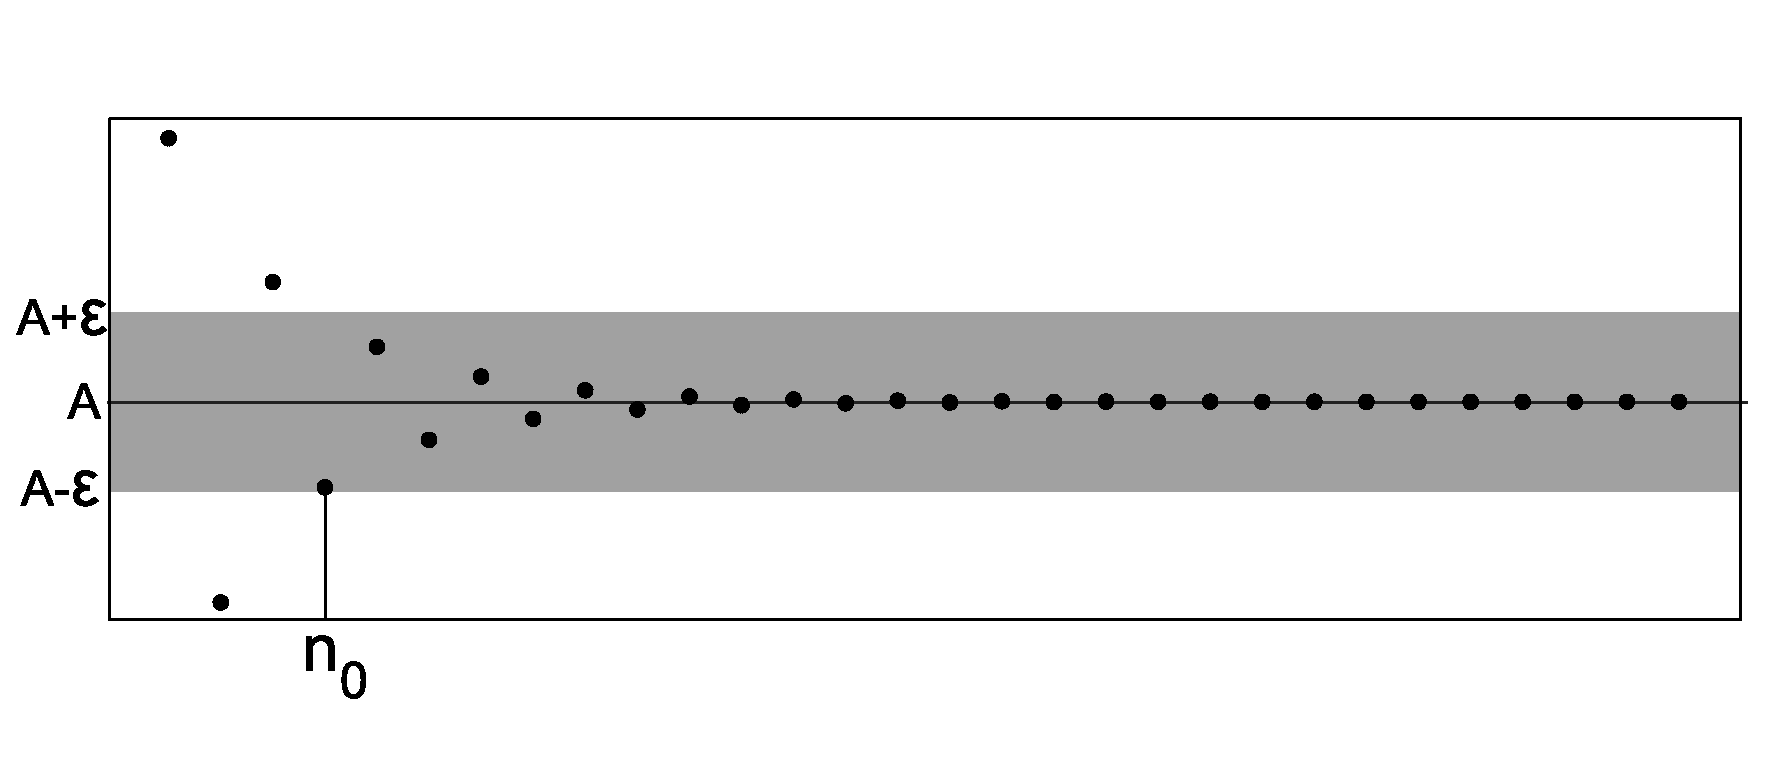
\includegraphics[width=145mm]{matematika/obrazky/02-limita}
\caption{Ilustrace k definici vlastn� limity}
\label{fig:limita_posloupnosti}
\end{figure}

\begin{poznamka}
Na obr�zku \ref{fig:limita_posloupnosti} jsem nakreslil posloupnost k osv�tlen� definice limity. Jde o posloupnost\footnote{konkr�tn� $a_0=1, a_n=\cos a_{n-1}$, ale nen� to d�le�it�}, kter� konverguje k ��slu $0.739085$, ozna�eno $A$. 

Pro ilustraci \uv{libovoln� mal�ho $\varepsilon$} (m��eme ��ci \uv{libovoln� velk�ho}, ale my chceme naopak $\varepsilon$ co \emph{nejmen��}) jsem do stejn�ho obr�zku nazna�il dv� r�zn� $\varepsilon$ --- proto�e vzd�lenost je \uv{na ob� strany}, jsou obd�ln�ky \uv{vysok�} $2\varepsilon$ --- a pro ka�d� z nich jsem na�el takov� $n_0$, �e pro $n\ge n_0$ u� jsem v�dy od $A$ vzd�len maxim�ln� $\varepsilon$.
\end{poznamka}


\begin{definice}
Jestli�e existuje $A \in \mathbb{R}$ tak, �e $\lim_{n \rightarrow \infty}a_n = A$, pak ��k�me, �e posloupnost $\{a_n\}$ m� \emph{vlastn� limitu} nebo �e \emph{konverguje} (je \emph{konvergentn�}). V opa�n�m p��pad� ��k�me, �e posloupnost \emph{diverguje}.
\end{definice}

\begin{pozorovani}
Ne ka�d� posloupnost je konvergentn�. Nap��klad posloupnost 0,1,0,1,0,... nem� vlastn� limitu a podobn� posloupnost $\{2^n\}$ nem� vlastn� limitu.
\end{pozorovani}

\begin{priklady}
\begin{pitemize}
	\item $\lim_{n \rightarrow \infty} (\sqrt{n+1} - \sqrt{n}) = 0$
	\item $\lim_{n \rightarrow \infty} \sqrt[n]{n} = 1$
\end{pitemize}
\end{priklady}

\begin{poznamka}
N�sleduj�c� v�ty maj� pom�rn� lehk� d�kazy, kter� zde uv�d�t nebudu; pokud si je budete zkou�et, je dobr� si u nich uv�domit z�kladn� vlastnosti absolutn� hodnoty:
\begin{pitemize}
	\item $\left|a \cdot b\right|= \left|a\right| \cdot\left| b\right|$
	\item $\left|a + b\right| \leq \left|a\right| + \left| b\right|$
	\item $\left|a \right| \leq b\Leftrightarrow -b \leq a \leq b$
\end{pitemize}
\end{poznamka}

\begin{vetaN}{o jednozna�nosti limity posloupnosti}
Ka�d� posloupnost m� nejv��e jednu limitu.
\end{vetaN}

\begin{vetaN}{o omezenosti konvergentn� posloupnosti}
Ka�d� konvergentn� posloupnost je omezen�.
\end{vetaN}

\begin{definice}
Nech� $\{a_n\}_{n \in \mathbb{N}}$ je posloupnost re�ln�ch ��sel. �ekneme, �e posloupnost $\{b_k\}_{k \in \mathbb{N}}$ je \emph{vybran�} z posloupnosti, neboli �e posloupnost $\{b_k\}_{k \in \mathbb{N}}$ je \emph{podposloupnost�} posloupnosti $\{a_n\}_{n \in \mathbb{N}}$, jestli�e existuje rostouc� posloupnost p�irozen�ch ��sel $\{n_k\}$ takov�, �e $b_k = a_{n_k}$ pro v�echna $k \in \mathbb{N}$.
\end{definice}

\begin{vetaN}{o limit� vybran� posloupnosti}
Nech� $\{a_n\}_{n \in \mathbb{N}}$ je posloupnost re�ln�ch ��sel a nech� $\lim_{n \rightarrow \infty} a_n = A$. Nech� posloupnost $\{b_k\}_{k \in \mathbb{N}}$ je vybran� z posloupnosti $\{a_n\}_{n \in \mathbb{N}}$. Pak $\lim_{k \rightarrow \infty} b_k = A$.
\end{vetaN}

\begin{vetaN}{o aritmetice limit}
Nech� $\{a_n\}_{n \in \mathbb{N}}$ a $\{b_n\}_{n \in \mathbb{N}}$ jsou dv� posloupnosti re�ln�ch ��sel a nech� $\lim_{n \rightarrow \infty} a_n = A \in \mathbb{R}$ a $\lim_{n \rightarrow \infty} b_n = B \in \mathbb{R}$. Pak plat�:
\begin{penumerate}
	\item $\lim_{n \rightarrow \infty} (a_n+b_n) = A+B$
	\item $\lim_{n \rightarrow \infty} (a_n \cdot  b_n) = A\cdot B$
	\item je-li $\forall n \in \mathbb{N}: b_n \neq 0$ a $B \neq 0$, pak $\lim_{n \rightarrow \infty} \frac{a_n}{b_n}=\frac{A}{B}$
\end{penumerate}
\end{vetaN}

\begin{vetaN}{o limit� a uspo��d�n�}
Nech� $\{a_n\}_{n \in \mathbb{N}}$ a $\{b_n\}_{n \in \mathbb{N}}$ jsou dv� posloupnosti re�ln�ch ��sel a nech� $\lim_{n \rightarrow \infty} a_n = A \in \mathbb{R}$ a $\lim_{n \rightarrow \infty} b_n = B \in \mathbb{R}$. Pak plat�:
\begin{penumerate}
	\item Jestli�e $A < B$, potom $\exists n_0 \in \mathbb{N}\ \forall n > n_0: a_n < b_n$
	\item Jestli�e $\exists n_0 \in \mathbb{N}\ \forall n \ge n_0: a_n \ge b_n$, pak $A \ge B$
\end{penumerate}

\noindent Pozor, ostrost nerovnost� v tomto p��pad� je d�le�it�.
\end{vetaN}

\begin{vetaN}{o policajtech}
Nech� $\{a_n\}_{n \in \mathbb{N}}$, $\{b_n\}_{n \in \mathbb{N}}$ a $\{c_n\}_{n \in \mathbb{N}}$ jsou posloupnosti re�ln�ch ��sel, spl�uj�c�
\begin{penumerate}
	\item $\exists n_0 \in \mathbb{N}\ \forall n > n_0: a_n \le c_n \le b_n$
	\item $\lim_{n \rightarrow \infty}a_n = \lim b_n = A \in \mathbb{R}$
\end{penumerate}
Pak
$$
\lim c_n = A
$$
\end{vetaN}

\begin{vetaN}{o limit� sou�inu mizej�c� ($\lim=0$) a omezen� posloupnosti}
Nech� $\{a_n\}_{n \in \mathbb{N}}$ a $\{b_n\}_{n \in \mathbb{N}}$ jsou posloupnosti re�ln�ch ��sel, nech� je $\lim_{n \rightarrow \infty} a_n = 0$ a $\{b_n\}$ omezen�. Pak
$$
\lim_{n \rightarrow \infty}(a_n \cdot b_n) = 0
$$
\end{vetaN}

\subsubsection{Nevlastn� limity}
\begin{definice}
�ekneme, �e posloupnost  $\{a_n\}$ m� \emph{nevlastn� limitu} $+ \infty$, jestli�e:
$$ \forall K \in \mathbb{R}\ \exists n_0 \in \mathbb{N}: \forall n \ge n_0, n \in \mathbb{N}: a_n \ge K $$

Obdobn� �ekneme, �e posloupnost  $\{a_n\}$ m� \emph{nevlastn� limitu} $- \infty$, jestli�e:
$$ \forall K \in \mathbb{R}\ \exists n_0 \in \mathbb{N}: \forall n \ge n_0, n \in \mathbb{N}: a_n \le K $$

M�-li posloupnost nevlastn� limitu, ��k�me o n�, �e diverguje, stejn� jako v p��pad�, �e ��dnou limitu nem�.
\end{definice}

\begin{figure}
\centering%
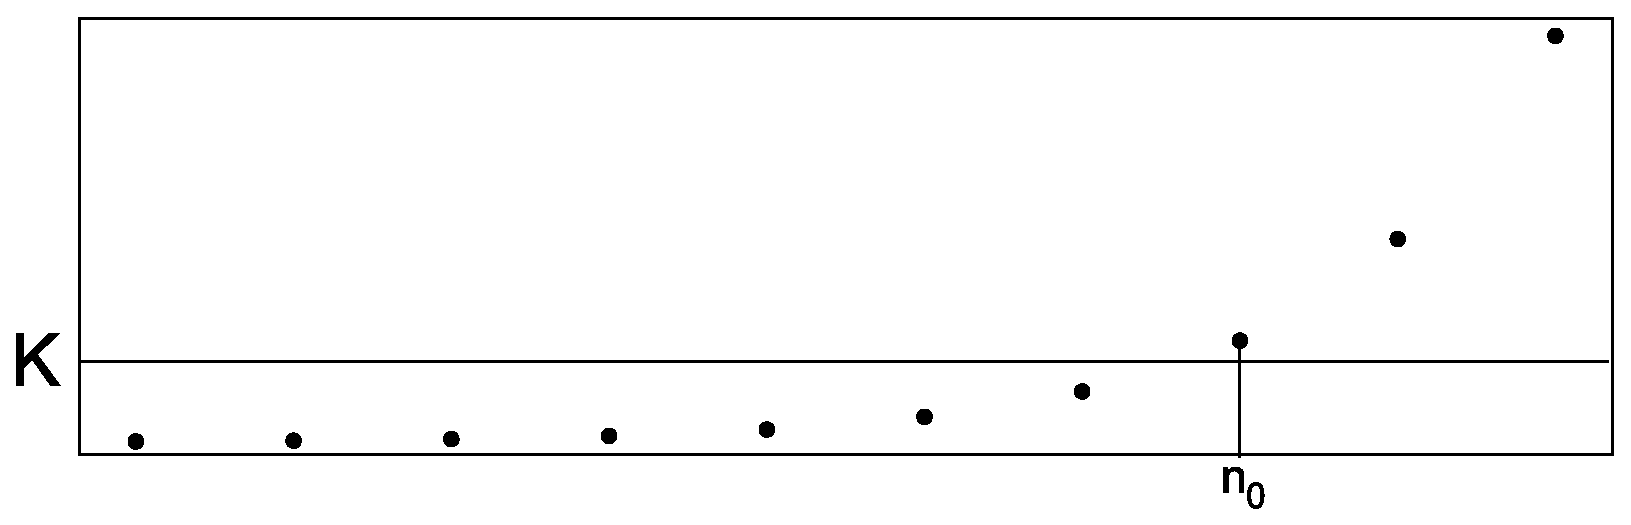
\includegraphics[width=145mm]{matematika/obrazky/03-limita_nevlastni}
\caption{Ilustrace k definici nevlastn� limity}
\label{fig:limita_nevlastni}
\end{figure}

\begin{poznamka}
Ilustrace k definici nevlastn� limity je na obr�zku \ref{label:limita_nevlastni}.
\end{poznamka}

\begin{poznamka}
V�echny mo�n� situace jsou zn�zorn�ny na n�sleduj�c�m diagramu:

limita posloupnosti:
\begin{pitemize}
	\item neexistuje
	\item existuje
	\begin{pitemize}
		\item vlastn�
		\item nevlastn�
		\begin{pitemize}
			\item $- \infty$
			\item $+ \infty$
		\end{pitemize}
	\end{pitemize}
\end{pitemize}

\end{poznamka}

\begin{definice}
Mno�inu $\mathbb{R}^* := \mathbb{R} \cup \{ + \infty, - \infty \}$ naz�v�me \emph{roz���enou re�lnou osou}.
\end{definice}

\begin{poznamka}
V�ty o jednozna�nosti limity, o limit� vybran� posloupnosti, o limit� a uspo��d�n� a o policajtech plat� v nezm�n�n� podob�, jestli�e p�ipust�me nevlastn� limity. V�ta o omezenosti konvergentn� posloupnosti zrejm� neplat� - nebo� je-li $\lim_{n \rightarrow \infty} a_n=\infty$ (nebo $- \infty$), pak posloupnost $\{a_n\}$ nen� omezen�; je ale omezen� \emph{zdola} u $\infty$ a \emph{shora} u $- \infty$. V�tu o aritmetice limit pro roz��renou osu uvedeme zvl᚝.
\end{poznamka}

\begin{vetaN}{o aritmetice limit pro nevlastn� limity}
Nech� $\{a_n\}_{n \in \mathbb{N}}$ a $\{b_n\}_{n \in \mathbb{N}}$ jsou dv� posloupnosti re�ln�ch ��sel a nech� $\lim_{n \rightarrow \infty} a_n = A \in \mathbb{R}^*$ a $\lim_{n \rightarrow \infty} b_n = B \in \mathbb{R}^*$. Pak plat�:
\begin{penumerate}
	\item $\lim_{n \rightarrow \infty} (a_n+b_n) = A+B \textit{, pokud je v�raz A+B definov�n}$
	\item $\lim_{n \rightarrow \infty} (a_n \cdot  b_n) = A\cdot B\textit{, pokud je v�raz }A\cdot B\textit{ definov�n}$
	\item je-li $\forall n \in \mathbb{N}: b_n \neq 0$ a $B \neq 0$, pak $\lim_{n \rightarrow \infty} \frac{a_n}{b_n}=\frac{A}{B} \textit{, pokud je v�raz } \frac{A}{B} \textit{ definov�n}$
\end{penumerate}
\end{vetaN}

\begin{definiceN}{Supremum a infimum na roz���en� re�ln� ose}
\begin{pitemize}
	\item Nech� mno�ina $A \subset \mathbb{R}$ je shora neomezen�. Pak klademe $\sup A := +\infty$
	\item Nech� mno�ina $A \subset \mathbb{R}$ je zdola neomezen�. Pak klademe $\inf A := -\infty$
	\item Nech� $A=\emptyset$. Pak klademe $\sup A := -\infty$ a $inf A := +\infty$
\end{pitemize}
\end{definiceN}

\begin{poznamka}
Pr�zdn� mno�ina je jedin� mno�ina, jej� supremum je men�� ne� jej� infimum.
\end{poznamka}

\begin{vetaN}{o limit� pod�lu kladn� a mizej�c� posloupnosti}
Nech� $\{a_n\}_{n \in \mathbb{N}}$ a $\{b_n\}_{n \in \mathbb{N}}$ jsou posloupnosti re�ln�ch ��sel, nech� je $\lim_{n \rightarrow \infty} a_n = A \in \mathbb{R}^*, A>0$ a nech� $\lim_{n \rightarrow \infty}\{b_n\}=0$. Nech�
$$
	\exists n_0 \in \mathbb{N} \textit{ } \forall n \ge n_0, n \in \mathbb{N}: b_n>0
$$
Pak
$$
	\lim_{n \rightarrow \infty} \frac{a_n}{b_n} = + \infty
$$
\end{vetaN}

\subsubsection{Monot�nn� posloupnosti}
\begin{vetaN}{o limit� monot�nn� posloupnosti}
Ka�d� monot�nn� posloupnost m� limitu.

\medskip\begin{dukaz}
Nazna�en� d�kazu: nap�. rostouc� posloupnost bu� nen� shora omezen� a m� tedy limitu $\infty$, nebo je shora omezen�, proto�e je ale z�rove� rostouc�, tak se k dan�mu horn�mu omezen� postupn� p�ibli�uje.
\end{dukaz}

\end{vetaN}

\begin{poznamka}
Je-li posloupnost neklesaj�c� (nerostouc�) a nav�c shora (zdola) omezen�, pak m� vlastn� limitu.
Je-li posloupnost neklesaj�c� (nerostouc�) a nav�c shora (zdola) neomezen�, pak m� limitu $+ \infty$ ($- \infty$).
\end{poznamka}

\begin{definiceN}{Limes superior a limes inferior}
Nech� $\{a_n\}_{n \in \mathbb{N}}$ je posloupnost re�ln�ch ��sel. Je-li $\{a_n\}$ shora omezen�, definujeme posloupnost $\{b_n\}_{n \in \mathbb{N}}$ p�edpisem:
$$
	b_n := \sup\{a_k; k \ge n \}
$$
Je-li $\{a_n\}$ zdola omezen�, definujeme posloupnost $\{c_n\}_{n \in \mathbb{N}}$ p�edpisem:
$$
	c_n := \inf\{a_k; k \ge n \}
$$
V takov�m p��pad� definujeme:
$$
\lim \sup~a_n := \left\{
\begin{array}{ll} \lim_{n \rightarrow \infty} b_n & \textit{jestli�e je } \{a_n\} \textit{ shora omezen�} \\ \infty & \textit{jestli�e je } \{a_n\} \textit{ shora neomezen�} \end{array}
\right.
$$
Tuto hodnotu naz�v�me \emph{limes superior} posloupnosti $\{a_n\}_{n \in \mathbb{N}}$. Obdobn� definujeme \emph{limes inferior} posloupnosti $\{a_n\}_{n \in \mathbb{N}}$ p�edpisem:
$$
\lim \inf~a_n := \left\{
\begin{array}{ll} \lim_{n \rightarrow \infty} c_n & \textit{jestli�e je } \{a_n\} \textit{ zdola omezen�} \\ - \infty & \textit{jestli�e je } \{a_n\} \textit{ zdola neomezen�} \end{array}
\right.
$$
\end{definiceN}

\begin{poznamka}
Limes superior a limes inferior jsou v�dy dob�e definovan� hodnoty a plat�
$$
\lim \sup~a_n \in \mathbb{R}^*, \lim \inf~a_n \in \mathbb{R}^*, 
$$
Na rozd�l od limity, kter� nemus� existovat, tyto dv� hodnoty existuj� pro
libovolnou posloupnost re�ln�ch ��sel.
\end{poznamka}

\begin{vetaN}{o vztahu limity, limes superior a limes inferior}
Nech� $\{a_n\}_{n \in \mathbb{N}}$ je posloupnost re�ln�ch ��sel. Potom 
$$
	\lim a_n = A \in \mathbb{R}^{*}
$$
pr�v� tehdy, kdy�
$$
\lim \sup~a_n = \lim \inf~a_n = A \in \mathbb{R}^*
$$
\end{vetaN}

\begin{definice}
Nech� $\{a_n\}_{n \in \mathbb{N}}$ je posloupnost re�ln�ch ��sel. Pak $A \in \mathbb{R}^*$ nazveme \emph{hromadnou hodnotou} posloupnosti $\{a_n\}$, jestli�e existuje vybran� posloupnost takov� $\{a_{n_k}\}$, �e $\lim_{k \rightarrow \infty} a_{n_k} = A$. Mno�ina v�ech hromadn�ch hodnot zna��me $H(\{a_n\})$
\end{definice}

\begin{vetaN}{o vztahu limes superior, limes inferior a hromadn�ch hodnot}
Nech� $\{a_n\}_{n \in \mathbb{N}}$ je posloupnost re�ln�ch ��sel. Potom $H\{(a_n)\} \neq \emptyset$,
$$
\lim \sup~a_n = \max H(\{a_n\}) \textit{ a } \lim \inf~a_n = \min H(\{a_n\})
$$
\end{vetaN}

\subsection{Cauchyovsk� posloupnosti}

Tato sekce je vypracovan� podle skript Prof. A. Pultra z matematick� anal�zy\\
(\texttt{http://kam.mff.cuni.cz/\~{}pultr/})
\bigskip

\begin{definiceN}{Bolzano-Cauchyova podm�nka}
�ekneme, �e posloupnost $\{a_n\}_{n\geq 0}$ je \emph{cauchyovsk�}, nebo-li �e spl�uje \emph{Bolzano-Cauchyho podm�nku}, pokud pro n� plat�:
$$
\forall \varepsilon > 0~~\exists n_0 \in \mathbb{N}: \forall m, n \in \mathbb{N}: m \ge n_0, n \ge n_0: |a_n - a_m| < \varepsilon
$$
\end{definiceN}

\begin{vetaN}{Bolzano-Weierstrassova}
Z ka�d� omezen� posloupnosti lze vybrat konvergentn� podposloupnost. Jsou-li $a_n$ v kompaktn�m intervalu $[a,b]$, je limita vybran� posloupnosti v tomto intervalu.

\medskip\begin{dukaz}
Prvn� ��st dok�eme nalezen�m takov� posloupnosti. Vezmeme $A:=\lim\sup~a_n$ a definujeme pro ka�d� $k\in\mathbb{N}$ mno�inu $M_k:=\{j\in\mathbb{N}|j>n_{k-1},a_j\in\langle A - \frac{1}{2^k}, A + \frac{1}{2^k}\rangle\}$ a $n_k:=\min M_k$. Potom $\{a_{n_k}\}$ je vybran� posloupnost, kter� konverguje. Druh� ��st je p��m�m d�sledkem v�ty o limit� a uspo��d�n�.
\end{dukaz}
\end{vetaN}

\begin{lemma}
M�-li cauchyovsk� posloupnost konvergentn� podposloupnost, je konvergentn�.

\medskip\begin{dukaz}
Nech� $\lim a_{n_k} = x$. Pro $\varepsilon > 0$ zvolme $n_0$, aby pro $m,n\geq n_0$ platilo $|a_m-a_n|<\frac{\varepsilon}{2}$ a $|a_k-x|<\frac{\varepsilon}{2}$. Proto�e $k_n\geq n$, plat� $|a_n-x|=|a_n-a_{k_n}|+|a_{k_n}-x|<\varepsilon$.
\end{dukaz}
\end{lemma}


\begin{vetaN}{Bolzano-Cauchyova}
Posloupnost $\{a_n\}$ m� vlastn� limitu, pr�v� kdy� je cauchyovsk�.

\medskip\begin{dukaz}
\begin{penumerate}
    \item Implikace \uv{$\Rightarrow$} je hned vid�t -- sta�� vz�t k $\varepsilon$ takov� $n_0$, �e $|a_n-x|<\frac{\varepsilon}{2}\ \forall n\geq n_0$. Potom je $|a_n-a_m|=|a_n-x+x-a_m|\leq|a_n-x|+|x-a_m|\leq\varepsilon\ \forall m,n\geq n_0$.\medskip
    \item Pro druhou implikaci sta�� dok�zat, �e je cauchyovsk� posloupnost omezen� a zbytek dostaneme z p�edchoz�ho lemmatu a Bolzano-Weierstrassovy v�ty. Pro $\varepsilon=1$ existuje $n_0$ takov�, �e $a_{n_0}-1<a_n<a_{n_0}+1$ pro ka�d� $n\geq n_0$ (to plyne p��mo z podm�nky), tak�e zb�v� jen kone�n� po�et �len� mimo toto rozmez� (pro $n<n_0$), a ty v�dy tvo�� omezen� syst�m.
\end{penumerate}
\end{dukaz}
\end{vetaN}


\newpage
\def\tg{\mathrm{tg}}
\def\cotg{\mathrm{cotg}}
\def\arctg{\mathrm{arctg}}
\def\arccotg{\mathrm{arccotg}}

\section{Z�klady diferenci�ln�ho po�tu}

\begin{e}{Po�adavky}{0}{0}
\begin{pitemize}
        \item Re�ln� funkce jedn� re�ln� prom�nn�
        \item Spojitost, limita funkce v bod� (vlastn� i nevlastn�)
        \item N�kter� konkr�tn� funkce (polynomy, racion�ln� lomen� funkce, goniometrick� a cyklometrick� funkce, logaritmy a exponenci�ln� funkce)
        \item Derivace: definice a z�kladn� pravidla, v�ty o st�edn� hodnot�, derivace vy���ch ��d�
        \item N�kter� aplikace (pr�b�hy funkc�, Newtonova metoda hled�n� nulov�ho bodu, Taylor�v polynom se zbytkem)
\end{pitemize}
\end{e}

\subsection{Re�ln� funkce jedn� re�ln� prom�nn�}
\begin{e}{Definice}{0}{Re�ln� funkce}
Re�ln� funkce jedn� prom�nn� je zobrazen� $f: M \rightarrow \mathbb{R}$, kde $M \subseteq \mathbb{R}$. \\
$f$ m��e b�t na $M$:
\begin{pitemize}
        \item \emph{rostouc�}: $\forall x, y: x < y \Rightarrow f(x) < f(y)$
        \item \emph{klesaj�c�}: $\forall x, y: x < y \Rightarrow f(x) > f(y)$
        \item \emph{neklesaj�c�}: $\forall x, y: x < y \Rightarrow f(x) \le f(y)$
        \item \emph{nerostouc�}: $\forall x, y: x < y \Rightarrow f(x) \ge f(y)$

        \item \emph{sud�}: $x \in M \Rightarrow -x \in M \wedge f(x)=f(-x), \forall x \in M$
        \item \emph{lich�}: $x \in M \Rightarrow -x \in M \wedge f(x)=-f(-x), \forall x \in M$
        \item \emph{periodick�} s periodou $p\in\mathbb{R}$: $x \in M \Rightarrow x \pm p \in M \wedge f(x)=f(x+p)=f(x-p), \forall x \in M$
\end{pitemize}
\end{e}

\begin{e}{Definice}{0}{Okol� bodu}
    \begin{pitemize}
        \item $P(a, \delta) = (a-\delta, a) \cup (a, a+\delta)$  \hfill \emph{(prstencov� okol�)} \hspace{0.4\textwidth}

        \item $P^{+}(a, \delta)=(a, a+\delta)$  \hfill \emph{(prav� prstencov� okol�)} \hspace{0.4\textwidth}

        \item $P^{-}(a, \delta)=(a-\delta, a)$  \hfill \emph{(lev� prstencov� okol�)} \hspace{0.4\textwidth}
        
        \item $B(a, \delta)=(a-\delta, a+\delta) = P(a, \delta)\cup\{a\}$ \hfill \emph{($\delta$-okol�)} \hspace{0.4\textwidth}

        \item $B^{+}(a, \delta)=P^{+}(a, \delta)\cup\{a\}$ \hfill \emph{(prav� $\delta$-okol�)} \hspace{0.4\textwidth}
        
        \item $B^{-}(a, \delta)=P^{-}(a, \delta)\cup\{a\}$ \hfill \emph{(lev� $\delta$-okol�)} \hspace{0.4\textwidth}
        
        \item $P(\infty, d) = B(\infty,d)=(\frac{1}{d}, \infty)$
        \item $P(-\infty, d) = B(-\infty,d)=(-\infty, -\frac{1}{d})$
\end{pitemize}
\end{e}

\subsection{Spojitost, limita funkce v bod� (vlastn� i nevlastn�)}

\obrazekvpravominipage{matematika/obrazky/limita_funkce}{Ilustrace limity}{fig:limitafunkce}{0.6}{0.4} {

\begin{e}{Definice}{0}{Limita}

�ekneme, �e $f$ m� v bod� $a \in \mathbb{R}^{*}$ limitu $A \in \mathbb{R^{*}}$, jestli�e
$$\forall \varepsilon>0\ \exists \delta>0: x \in P(a, \delta) \Rightarrow f(x) \in B(A, \varepsilon)$$
a zna��me $\lim_{x \rightarrow a} f(x) = A$

\medskip
Plat�-li tato vlastnost jen pro prav� okol� bod� $a$ a $A$, mluv�me o \emph{jednostrann� limit� zprava} a podobn� zleva.
\end{e}

\begin{e}{Definice}{0}{Spojitost v bod�}

�ekneme, �e $f$ je spojit� v bod� $a \in \mathbb{R}$, jestli�e  $$\lim_{x \rightarrow a} f(x) = f(a)$$

\end{e}

Na obr�zku \ref{fig:limitafunkce} je funkce, definovan� v�ude jako $f(x)=\mathrm{e}^x$ krom� bodu $a$, kde je definov�na jako $f(a)=Z \neq \mathrm{e}^a$. V~bod� $a$ m� limitu $A$ - pro r�zn� $\varepsilon$ nal�z�m p��slu�n� $\delta$; v~tomto bod� ale \emph{nen� spojit�}. Pokud by ale v~bod� $a$ byla $A$, byla by spojit�.

}

\medskip
\begin{e}{V�ta}{1}{Heineho v�ta}
Nech�  $f: M \rightarrow \mathbb{R}, M \subseteq \mathbb{R}$. Nech� $f$ je definov�no na n�jak�m prstencov�m okol� bodu $a \in \mathbb{R}^{*}$. Potom n�sleduj�c� dv� tvrzen� jsou ekvivalentn�:
\begin{penumerate}
        \item $lim_{x \rightarrow a} f(x) = A \in \mathbb{R}^{*}$
        \item Pro ka�dou posloupnost $\{x_n\}_{n=1}^{\infty}$ spl�uj�c� $x_n \in D(f)\ \forall n \in \mathbb{N}$ a  $\lim x_n = a, x_n \neq a\ \forall n$ plat� $\lim_{n \rightarrow \infty} f(x_n)=A$
\end{penumerate}
Heineho v�ta umo��uje tvrzen�, vysloven� o limit�ch posloupnost�, p�ev�d�t na limity funkc� v bod�.

\begin{e}{Idea d�kazu}{0}{0}
    (nejsem si jist, jestli d�kaz funguje i pro nekone�na)
    
    1$\Rightarrow$2 Pro $\varepsilon$ okol� $A$ najdu odpov�daj�c� $\delta$ okol� $a$, $x_n$ jsou od n�jak�ho $n_0$ v�echny v~tomto $\delta$ okol�, jejich obrazy ale mus� b�t i v~$\varepsilon$ okol� $A$ .
    
    2$\Rightarrow$1 Sporem. Mus� existovat $\varepsilon$, �e $\forall \delta \exists x \in P(a, \delta)$ takov�, �e $f(x) \notin B(A, \varepsilon)$ (pouze negace definice limity). M��eme tedy postupn� zmen�ovat $\delta$, v~ka�d�m $ P(a, \delta)$ naj�t takov� $x$ a vytvo�it tak posloupnost, kter� m� limitu v~$a$, ale jej� obrazy nebudou m�t limitu v~$A$, proto�e jsou v�dy vzd�len� $\varepsilon$ -- spor.
\end{e}
\end{e}

\begin{e}{V�ta}{0}{V�ta o jednozna�nosti limity funkce}
Funkce $f$ m� v ka�d�m bod� nejv��e jednu limitu.

\begin{e}{Idea d�kazu}{0}{0}
    Bu� p��mo, nebo p�es Heineho v�tu a u� dok�zan� vlastnosti limit posloupnost�.
\end{e}
\end{e}

\begin{e}{V�ta}{0}{O lok�ln� omezenosti funkce s vlastn� limitou}
Nech� funkce $f$ m� v bod� $a \in \mathbb{R}^{*}$ vlastn� limitu. Potom existuje $\delta > 0$ takov�, �e $f$ je na $P(a, \delta)$ omezen�.

\begin{e}{Idea d�kazu}{0}{0}
    Bu� p��mo, nebo p�es Heineho v�tu a u� dok�zan� vlastnosti limit posloupnost�.
\end{e}

\end{e}

\begin{e}{V�ta}{0}{Aritmetika limit pro funkce}
Nech� $\lim_{x \rightarrow a} f(x)=A$, $\lim_{x \rightarrow a} g(x)=B$, $a \in R^{*}$. Potom
\begin{penumerate}
        \item $\lim (f(x)+g(x)) = A+B$, je-li v�raz na prav� stran� definov�n.
        \item $\lim (f(x)g(x)) = A\cdot B$, je-li v�raz na prav� stran� definov�n.
        \item $\lim \frac{f(x)}{g(x)} = \frac{A}{B}$, je-li v�raz na prav� stran� definov�n.
\end{penumerate}

\begin{e}{Idea d�kazu}{0}{0}
    Bu� p��mo, nebo p�es Heineho v�tu a u� dok�zan� vlastnosti limit posloupnost�.
\end{e}

\end{e}

\begin{e}{V�ta}{0}{Limita a uspo��d�n� - policajti pro funkce}
\begin{penumerate}
        \item Nech� $\lim_{x \rightarrow a} f(x) > \lim_{x \rightarrow a} g(x)$, $a \in R^{*}$.\\Potom $\exists P(a, \delta): f(x)>g(x) \ \forall x \in P(a, \delta)$
        \item Nech� $f(x) \le g(x), \forall x \in P(a, \delta), \delta > 0$ a existuj� $\lim_{x \rightarrow a} f(x)$, $\lim_{x \rightarrow a} g(x)$.\\Potom $\lim_{x\to a} f(x) \le \lim_{x\to a} g(x)$.
        \item Nech� $f(x) \le h(x) \le g(x), \forall x \in P(a, \delta), \delta > 0$ a $\lim_{x \rightarrow a} f(x) = \lim_{x \rightarrow a} g(x)$.\\Potom existuje $\lim h(x)$ a $\lim_{x \rightarrow a} h(x) = \lim_{x \rightarrow a} f(x) = \lim_{x \rightarrow a} g(x)$.
\end{penumerate}
Pozor na ostrost nerovnost�, v tomto p��pad� je velmi d�le�it�.

\begin{e}{Idea d�kazu}{0}{0}
    Bu� p��mo, nebo p�es Heineho v�tu a u� dok�zan� vlastnosti limit posloupnost�.
\end{e}

\end{e}

\begin{e}{Definice}{0}{Jednostrann� spojitost funkce v bod�}
\begin{pitemize}
        \item $\textit{funkce f je spojit� v a} \Leftrightarrow \lim_{x \rightarrow a} f(x)=f(a) \Leftrightarrow \forall \varepsilon>0~\exists \delta >0: f(B(a, \delta)) \subseteq B(f(a), \varepsilon)$
        \item $\textit{funkce f je spojit� v a zprava} \Leftrightarrow \lim_{x \rightarrow a^{+}} f(x)=f(a) \Leftrightarrow \forall \varepsilon>0~\exists \delta >0: f(B^{+}(a, \delta)) \subseteq B(f(a), \varepsilon)$
        \item $\textit{funkce f je spojit� v a zleva} \Leftrightarrow \lim_{x \rightarrow a^{-}} f(x)=f(a) \Leftrightarrow \forall \varepsilon>0~\exists \delta >0: f(B^{-}(a, \delta)) \subseteq B(f(a), \varepsilon)$
\end{pitemize}
\end{e}

\obrazekvpravominipage{matematika/obrazky/protipriklad_slozena}{Protip��klad na podm�nky o limit�}{fig:protipriklad_slozena}{0.4}{0.6}{

\begin{e}{V�ta}{0}{O limit� slo�en� funkce}
Nech� $\lim_{x \rightarrow a} g(x) = A$, $\lim_{y \rightarrow A} f(y) = B$, $a, A, B \in \mathbb{R}^{*}$. Nech� nav�c plat� jeden z p�edpoklad�:\\
(P1) $f$ je spojit� v $A$\hfill \emph{(vn�j�� funkce je spojit�)} 

(P2) $\exists \delta > 0: g(x) \neq A$ pro $\forall x \in P(a, \delta)$\hfill \emph{(vnit�n� je \uv{lok�ln� prost�})}

Potom $\lim_{x \rightarrow a} (f \circ g)(x) = B$.

\begin{e}{Pozn�mka}{0}{protip��klad}
        Na obr�zku \ref{fig:protipriklad_slozena} je uveden protip��klad pro osv�tlen�, pro� mus� podm�nky platit. $f(x)$ -- vn�j�� -- je nespojit�, $g(x)$ -- vnit�n� -- nen� lok�ln� prost�. Slo�en� funkce potom nem� v~bod� $-1$ limitu -- a tam, kde j� m�, se stejn� \emph{nerovn�} slo�en� limit� (limita $f(x)$ v~nule je 1, ale limita $f(g(x))$ je v~nule 0 a dokonce je tam i spojit�). \uv{Pouh�}�bod nespojitosti vn�j�� funkce se n�sledkem konstantnosti vnit�n� funkce \uv{rozt�hnul}.
\end{e}

\begin{e}{Idea d�kazu}{0}{0}
  Vezmeme $\varepsilon$, pro n�j najdeme $\mu$, �e pro $x$ z~okol� $A$ je $f(x)$ v~$\varepsilon$ okol� -- ale pozor, definice limity je $0 < \left|x-A\right| < \mu \Rightarrow \left|f(x)-B\right|<\varepsilon$. M��eme z~definice limity $g(x)$ naj�t $\delta$�pro $\mu$, �e $0 < \left|g-a\right| < \delta \Rightarrow \left|g(x)-A\right|<\mu$. 

Pokud plat� (P2), $\left|g(x)-A\right|$ nikdy nebude 0, tak�e lev� strana plat� a t�m p�dem jsme ve vysn�n�m $\varepsilon$; pokud plat� (P1), 0 to b�t m��e, ale d�ky spojitosti jsme zase v~klidu a bezpe�� $\varepsilon$.
\end{e}

\end{e}
}

\begin{e}{Definice}{0}{Interval}
Nech� $a, b \in \mathbb{R}^{*}, a < b$. Pak \emph{otev�en�m intervalem} $(a, b)$ nazveme $\{x | a<x<b\}$, \emph{(uzav�en�m) intervalem} $\left<a, b\right>$ (pro $a, b \in \mathbb{R}$) nazveme $I=\{x | a \le x \le b\}$. Uzav�en� interval se n�kdy zna�� i $[a,b]$.
\end{e}

\begin{e}{V�ta}{0}{V�ta o limit� monot�nn� funkce}
Nech� je funkce $f$ monot�nn� na $(a, b)$, $a, b \in \mathbb{R}^{*}, a < b$. Potom $\exists \lim_{x \rightarrow a^{+}} f(x)$, $\exists \lim_{x \rightarrow b^{-}} f(x)$.

\begin{e}{Idea d�kazu}{0}{0}
    Bu� p��mo, nebo p�es Heineho v�tu a u� dok�zan� vlastnosti limit posloupnost� (omezen� a monot�nn� posloupnost m� limitu).
\end{e}

\end{e}

\begin{e}{Definice}{0}{Spojitost na intervalu}
Je-li $\left<a, b\right>$ interval, pak $a$ naz�v�me po��te�n�m bodem, $b$ koncov�m bodem a $x \in (a, b)$ vnit�n�mi body.

�ekneme, �e $f$ \emph{je spojit� na intervalu $I$}, jestli�e je spojit� zprava ve v�ech bodech krom� koncov�ho a spojit� zleva ve v�ech bodech krom� po��te�n�ho.
\end{e}


\obrazekvpravominipage{matematika/obrazky/darboux}{Darbouxova v�ta}{fig:darboux}{0.4}{0.6}{

\begin{e}{V�ta}{1}{Darbouxova o nab�van� mezihodnot}
Nech� funkce $f$ je spojit� na $\left<a, b\right>$ a $f(a)<f(b)$, potom $\forall y \in (f(a), f(b))$ existuje $x \in (a, b)$ takov�, �e $f(x)=y$.

Ilustrov�no na obr�zku \ref{fig:darboux}.

\begin{e}{Idea d�kazu}{0}{0}
K d�kazu se n�m bude hodit lemma, vypl�vaj�c� z~definice limity.

\begin{e}{Lemma}{0}{0}
Pokud m� spojit� funkce v $x_0$ hodnotu ost�e v�t�� ne� $y$, m� hodnotu $f(x)>y$ i v~n�jak�m okol� $x_0$. (vezmeme si chyt�e epsilon)
\end{e}

Pokra�ujeme s d�kazem Darbouxe.

M�jme $y$, pro n�j hledejme $x$, �e $f(x)=y$. Zkoumejme mno�inu v�ech hodnot, kter� maj� hodnotu men�� nebo rovnu, ne� $y$, tj. $M=\{x|f(x)\leq y\}$. Mno�ina $M$ je shora omezen� a tak m� supr�mum, nazveme ho $s$. Zkoumejme $f(s)$.

Pokud by hodnota $f(s)$ byla v�t��, ne� $y$, d�ky lemmatu by byla v�t�� i pro n�jak� men�� $x < s$ a tedy by ne�lo o nejmen�� horn� mez.

Pokud by hodnota $f(s)$ byla men��, ne� $y$, d�ky lemmatu by byla men�� i pro n�jak� v�t�� $x>s$ a tedy by ne�lo v�bec o horn� mez.

Hodnota $f(s)$ tedy mus� b�t $y$.

\end{e}

\end{e}
}

\begin{e}{V�ta}{0}{O spojit�m obrazu intervalu}
Nech� funkce $f: I \rightarrow \mathbb{R}$ je spojit� na intervalu $I$. Potom $f(I)$ je tak� interval.

\begin{e}{Idea d�kazu}{0}{0}
Pultr dokazuje p�es Darbouxe -- krajn� body $I$ tam maj� svoje hodnoty, v�echny hodnoty mezi t�mito hodnotami tam mus� b�t a proto je to interval. J� si nejsem �pln� jist�, ale budu Pultrovi v��it. V~kapitole o prostorech se beztak podobn� d�kazy opakuj�.

\end{e}
\end{e}

\begin{e}{Definice}{0}{0}
$f: M \rightarrow \mathbb{R}, M \subseteq \mathbb{R}$. $f$ nab�v� v bod� $a \in M$:
\begin{pitemize}
        \item \emph{maxima} na M $\Leftrightarrow \forall x \in M: f(x) \le f(a)$
        \item \emph{minima} na M $\Leftrightarrow \forall x \in M: f(x) \ge f(a)$
        \item \emph{ostr�ho maxima} na M $\Leftrightarrow \forall x \in M\setminus \{a\}: f(x) < f(a)$
        \item \emph{ostr�ho minima} na M $\Leftrightarrow \forall x \in M\setminus \{a\}: f(x) > f(a)$
        \item \emph{lok�ln�ho} maxima (minima, ostr�ho...)$\Leftrightarrow \exists \delta > 0: f$ nab�v� na $M \bigcap B(a, \delta)$ maxima (minima, ...)
\end{pitemize}
\end{e}

\begin{e}{V�ta}{0}{Vztah spojitosti a extr�m�}
Nech� $f$ je spojit� na $\left<a, b\right>$. Potom $f$ nab�v� na $\left<a, b\right>$ sv�ho maxima i minima.

\begin{e}{Idea d�kazu}{0}{0}
        Vezmeme si supr�mum hodnot, budeme kolem n�j zmen�ovat okol�, mus� tam v�dycky n�co b�t, tj. m�me posloupnost, z~n� vybereme konvergentn�, mus� konvergovat k~limit�, tam je to maximum. Minimum tot�.
\end{e}
\end{e}

\begin{e}{V�ta}{0}{Vztah spojitosti a omezenosti}
Spojit� funkce na uzav�en�m intervalu $\left<a, b\right>$ je omezen�.

\begin{e}{Idea d�kazu}{0}{0}
M� tam maximum i minumum, tj je omezen�.
\end{e}

\end{e}

\begin{e}{Definice}{0}{prost� funkce, inverzn� funkce}
Funkce $f$ je \emph{prost�}, jestli�e $\forall x, y \in D(f): x \neq y \Rightarrow f(x) \neq f(y)$.

Nech� $f$ je prost� na $M$, tedy $f: M \rightarrow f(M)$. Pak \emph{inverzn� funkce} $f^{-1}$ k funkci $f$ je definovan� na $f(M)$ p�edpisem: $y \in f(M)$, pak $f^{-1}(y)=x \Leftrightarrow y=f(x)$.
\end{e}

\begin{e}{V�ta}{0}{O inverzn� funkci}
Nech� $I$ je interval a funkce $f$ je definovan�, spojit� a rostouc� (klesaj�c�) na $I$. Potom inverzn� funkce $f^{-1}$ je definov�na, spojit� a rostouc� (klesaj�c�) na $f(I)$.
\end{e}

\begin{reportN}{Majerech}
Vyt�hl jsem si funkce jedn� prom�nn�... to nezn�lo �patn� co p�i�lo byl docela �ok... ot�zka byla toti�:
Doka�te v�tu o Darbouxouv� vlastnosti pro spojit� funkce - ��dn� v�ty nebo definice - prost� jeden d�kaz
uff d�kaz jsem nevid�l od prv�ku... no vymyslel jsem n�co co vypadalo d�v�ryhodn� 
majerech se pod�val konstatoval, �e takhle si d�kaz nep�edstavoval... a �e se to norm�ln� dokazuje jinak, uznal �e to co jsem vyrobil m� hlavu a patu nicm�n� pou�il jsem �e uzav�en� interval je kompaktn� mno�ina a �e tam lze tedy vybrat konvergentn� podposloupnost co� majerech prohl�sil �e je d�sledek toho co m�m dokazovat... a �e bych asi to m�l uk�zat... na�t�st� z toho se�lo po t�to co majerech po drobn�m p�esv�d�ov�n� uznal �e v�ta byla +- dok�z�na 
\end{reportN}


\begin{reportN}{Zahradn�k}
v podstate jen definice, Heineho veta a par pozorovani
 Zde jsem napsal definici spojitosti, tu v�tu, a p�ehled v�t a vlastnost� n�jak se vztahuj�c�ch k spojitosti. Napsal jsem zn�n� Darbouxovy v�ty + d�kaz. To sta�ilo. 
\end{reportN}

\begin{reportN}{IOI 21. 6. 2011 $<$2007}
1.1 Definujte pojem limity funkce v bode
\\
2.1 Urcete limitu funkc� $\sin(1/(x-1))$ a $(x-1)*\sin(1/(x-1))$ v bode 1
\end{reportN}

\subsection{N�kter� konkr�tn� funkce (polynomy, racion�ln� lomen� funkce, goniometrick� a cyklometrick� funkce, logaritmy a exponenci�ln� funkce)}

Teoreticky se daj� funkce popsat axiomaticky (s~t�m, �e jejich existence a jednozna�nost se dok�e pozd�ji). Nebo se daj� naopak zadefinovat konkr�tn� a axiomy z nich vyplynou jako jejich vlastnosti. Ono je to asi fuk -- d�kazy existenc� t�chto funkc� jsou tak jako tak na st�tnice p��li� slo�it� (podle m�).

\begin{e}{V�ta}{0}{Exponenci�ln� funkce}
Existuje pr�v� jedna re�ln� funkce \textbf{exp}, spl�uj�c�:
\begin{pitemize}
        \item $\exp(x+z)=\exp(x) \exp(z), \forall x,z \in \mathbb{R}$
        \item $\exp(x) \ge 1+x, \forall x \in \mathbb{R}$
\end{pitemize}
\end{e}

\begin{e}{Pozn�mka}{0}{N�kter� vlastnosti $\exp$}
Plat�:
\begin{pitemize}
    \item $\exp 0=1$
    \item $\exp (-x) = \frac{1}{\exp x}$
    \item $\exp (x) \neq 0\ \forall x\in \mathbb{R}$
    \item $\lim_{x\to\infty}\exp x=\infty$, $\lim_{x\to-\infty}\exp x=0$
    \item $\exp$ je rostouc� na $\mathbb{R}$
    \item $\lim_{x\to 0}\frac{\exp x - 1}{x}=1$
\end{pitemize}
\end{e}

\begin{e}{V�ta}{0}{Vlastnosti $\log$}
Funkce $\log$, definovan� p�edpisem $\log=\exp^{-1}$ m� n�sleduj�c� vlastnosti:
\begin{pitemize}
        \item $D(\log)=(0, \infty)$, $\log ((0, \infty)) \rightarrow \mathbb{R}$
        \item $\log(x\cdot y) = \log x + \log y, \forall x, y \in (0, \infty)$, $\log(x^n)=n\log x$
        \item log je spojit�, rostouc� na $(0, \infty)$, $\log 1=0$, $\log e = 1$
        \item $lim_{x \rightarrow 0_{+}} \log x = - \infty$, $lim_{x \rightarrow \infty} \log x = \infty$
        \item $lim_{x \rightarrow 1} \frac{\log x}{x-1} = 1$, $lim_{x \rightarrow 0} \frac{\log x+1}{x} = 1$
\end{pitemize}
\end{e}

\begin{e}{Definice}{0}{obecn� mocnina}
Obecn� mocnina $a^b=\exp(b \log a)$ pro $a>0, b \in \mathbb{R}$. Speci�ln� pro $a=e: e^x=\exp x$
\end{e}

\begin{e}{V�ta}{0}{0}
Existuje pr�v� jedna re�ln� funkce $s$ a pr�v� jedna re�ln� funkce $c$ takov�, �e:

\begin{pitemize}
        \item $s(x+y) = s(x)c(y) + c(x)s(y)$
        \item $c(x+y) = c(x)c(y) - s(x)s(y)$
        \item $s$ je lich�, $c$ sud�
        \item $s>0~\textit{na}~(0,1), s(1)=0$
\end{pitemize}
\end{e}

\begin{e}{Definice}{0}{0}
\noindent Podle $s$ a $c$ definujeme \emph{Goniometrick� funkce}:\\
$\sin(x)=s(\frac{x}{\pi})$, $\cos(x)=c(\frac{x}{\pi})$, $\tg(x)=\frac{\sin(x)}{\cos(x)}$, $\cotg(x)=\frac{\cos(x)}{\sin(x)}$

\noindent \emph{Cyklometrick� funkce}:
\begin{pitemize}
        \item $\arcsin x = y \Leftrightarrow y \in <-\frac{\pi}{2}, \frac{\pi}{2}> \wedge \sin y=x$
        \item $\arccos x = y \Leftrightarrow y \in <0, \pi> \wedge \cos y=x$
        \item $\arctg~x = y \Leftrightarrow y \in (-\frac{\pi}{2}, \frac{\pi}{2}) \wedge \tg~y=x$
        \item $\arccotg~x = y \Leftrightarrow y \in (0, \pi) \wedge \cotg~y=x$
\end{pitemize}

\noindent a plat�
$$\lim_{x \rightarrow 0} \frac{\arcsin x}{x} = 1$$
$$\lim_{x \rightarrow 0} \frac{\arccos x}{\sqrt{1-x}} = \lim_{x \rightarrow 0} \frac{\arctg x}{x} = 1$$
\end{e}

\subsection{Derivace: definice a z�kladn� pravidla, v�ty o st�edn� hodnot�, derivace vy���ch ��d�}
\obrazekvpravominipage{matematika/obrazky/derivace}{Derivace}{fig:derivace}{0.5}{0.5}{

\begin{e}{Definice}{0}{0}
Nech� $f$ je re�ln� funkce jedn� prom�nn�, $a \in \mathbb{R}$. Derivac� funkce $f$ v bod� $a$ nazveme
$$f'(a) = \lim_{h \rightarrow 0} \frac{f(a+h)-f(a)}{h} \textrm{, pokud existuje}$$

\noindent Derivac� zprava a zleva rozum�me:
$$f'_{+}(a) = \lim_{h \rightarrow 0_+} \frac{f(a+h)-f(a)}{h}, \, f'_{-}(a) = \lim_{h \rightarrow 0_-} \frac{f(a+h)-f(a)}{h}$$
\end{e}

Mo�n� trochu osv�tluj�c� obr�zek je \ref{fig:derivace} -- sna��me se o sm�rnici te�ny, sm�rnice je definov�na jako svisl� r�st d�leno vodorovn� r�st, sna��me se j� p�ibl�it.

}
\medskip
\begin{e}{V�ta}{0}{Vztah derivace a spojitosti}
M�-li $f$ v $a$ vlastn� (tj. kone�nou) derivaci, potom je $f$ v $a$ spojit�.


\begin{e}{Idea d�kazu}{0}{0}
        $\lim_{x\rightarrow a}(f(x)-f(a)) = \lim_{x\rightarrow a}\frac{f(x)-f(a)}{x-a}(x-a)=f'(x)\cdot 0 = 0$, $\lim_{x\rightarrow a}f(x)=\lim(f(x)-f(a)+f(a)) = f(a)$.
\end{e}

\end{e}

%Na dokazov�n� aritmetik jsem moc l�n�, to si ud�lejte sami :P je to v�t�inou nudn� po��t�n�

\begin{e}{V�ta}{0}{Aritmetika derivac�}
Nech� existuj� $f'(a)$, $g'(a)$:
\begin{penumerate}
        \item $(f+g)'(a)=f'(a)+g'(a)$, je-li prav� strana definov�na
        \item je-li $g$ nebo $f$ spojit� v $a$, pak $(fg)'(a)=f'(a)g(a)+f(a)g'(a)$
        \item je-li $g$ spojit� v $a$, $g(a) \neq 0$, pak $(\frac{f}{g})'(a)=\frac{f'(a)g(a)-f(a)g'(a)}{g^2(a)}$
\end{penumerate}

\begin{e}{D�kaz}{0}{0}

Je pracn�.

\end{e}

\end{e}

\begin{e}{V�ta}{0}{O derivaci slo�en� funkce}
Nech� funkce $f$ m� derivaci v $y_0$, $g$ m� derivaci v $x_0$, $g$ je spojit� v $x_0$ a $y_0=g(x_0)$. Potom $(f \circ g)'(x_0)=f'(y_0)\cdot g'(x_0)=f'(g(x_0))\cdot g'(x_0)$.


\begin{e}{Idea d�kazu}{0}{0}
        Je velmi pracn�, jen nazna��m. Zlomek uprav�me na

        $$\frac{f(g(x))-f(g(a))}{x-a}=\frac{f(g(x))*f(g(a))}{g(x)-g(a)}\cdot\frac{g(x)-g(a)}{x-a}.$$

        Rozlo��me na dv� mno�iny -- $A=\{x|g(x)\neq g(a)\}$, $B=\{x|g(x)= g(a)\}$. Ka�d� se mus� vy�e�it zvl᚝, d�ky spojitosti to ale jde.


\end{e}

\end{e}

\begin{e}{V�ta}{0}{O derivaci inverzn� funkce}
Nech� funkce $f$ je na intervalu $(a,b)$ spojit� a ryze monotonn�\footnote{aby v�bec m�la inverzn�}  a m� v bod� $x_0 \in (a,b)$ derivaci $f'(x_0)$ vlastn� a r�znou od nuly. Potom m� funkce $f^{-1}$ derivaci v bod� $y_0=f(x_0)$ a plat� rovnost
$$(f^{-1})'(y_0) = \frac{1}{f'(f^{-1}(y_0))}=\frac{1}{f'(x_0)}.$$
\begin{e}{Pozn�mka}{0}{0}
Pokud v situaci popsan� v pr�v� uveden� v�t� je $f'(x_0)$ nevlastn�, je $(f^{-1})'(y_0)=0$. Je-li $f'(x_0)=0$, je $(f^{-1})'(y_0)=+\infty$ (je-li $f$ rostouc�), resp. $=-\infty$ (je-li $f$ klesaj�c�).
\end{e}

\begin{e}{P��klad}{0}{0}
Definice nen� �pln� pr�hledn�. �ekn�me, �e zkoum�me funkci $f(x)=x^2$ na intervalu $(0,+\infty)$. V bod� $x_0=1$ m� derivaci $f'(x_0)=2x_0 = 2$. Funkce $f^{-1}$, tedy $\sqrt{y}$ m� derivaci v bod� $y_0=f(x_0)=x_0^2=1^2=1$ (to je bod, odkud zobrazujeme inverzn� funkci, ale kam dopad� hlavn� funkce, a kde zji��ujeme derivaci inverzn� funkce) a plat�, �e $\left(\sqrt{y}\right)'(y_0)=\frac{1}{\left(x^2\right)'(x_0)}=\frac{1}{2}$.

(nev�m, jak moc jsem to ujasnil :-))

\end{e}

\begin{e}{D�kaz}{0}{0}
Polo�me funkci $F(x)$ $$F(x) = \frac{x-x_0}{f(x)-f(x_0)}$$ (tj. \uv{obr�cen�} definice limity). Tato funkce m� z~definice limitu $\lim{x\rightarrow y}=\frac{1}{f'(x_0)}$. 

Proto�e $g(y)$ je prost� a spojit�, m��eme j� (d�ky Heineho v�t� a v�t� o slo�en�ch posloupnostech) vlo�it do $F(x)$ a bude platit $\lim_{y\rightarrow y_0} = \frac{1}{f'(x_0)}$ -- tj. tot�, jako p�edt�m (proto�e $g(y)=x$), ale jde o limitu podle $y$.

Tak� ale plat� $$F(g(y)) = \frac{g(x)-g(x_0)}{f(g(x))-f(g(x_0))} = \frac{g(x)-g(x_0)}{x-x_0}$$.
\end{e}

\end{e}

\begin{e}{V�ta}{0}{0}
Je-li v~bod� $x_0$ $f'(x_0)>0$, $f(x)$ v~bod� $x_0$ roste. Pokud je v~bod� tam $<0$, tak kles�..

\begin{e}{D�kaz}{0}{0}

Bu� t�eba $f'(x)=\lim_{x\rightarrow x_0}\frac{f(x)-f(x_0)}{x-x_0}>0$. Mus� b�t $>0$ na cel�m n�jak�m okol� -- v~bodech vpravo od $x_0$ je $x-x_0>0$ a tak i $f(x)-f(x_0)>0$, vlevo naopak.
\end{e}

\end{e}

\begin{e}{V�ta}{0}{Nutn� podm�nka lok�ln�ho extr�mu}
Nech� $M \subseteq \mathbb{R}$, $f: M \rightarrow \mathbb{R}$. Nech� $f$ m� v $a \in M$ lok�ln� extr�m. Pak bu� neexistuje $f'(a)$, nebo $f'(a)=0$.

\begin{e}{D�kaz}{0}{0}
Pokud existuje, tak v~cel�m okol� $f(x)$ ani nekles�, ani nestoup�, spolu s~p�edchoz� v�tou d�v�, �e tam mus� b�t 0.
\end{e}
\end{e}

\obrazekvpravominipage{matematika/obrazky/rolle}{Ilustrace Rolleovy v�ty}{fig:rolle}{0.4}{0.6}{
\begin{e}{V�ta}{1}{Rolleova v�ta}
Nech� $f$ je spojit� na $\left<a, b\right>$ a nech� existuje $f'(x)\ \forall x \in (a,b)$. Nech� $f(a)=f(b)$. Potom existuje $c \in (a,b): f'(c)=0$.


\begin{e}{Pozn�mka}{0}{0}
Rolleova v�ta je jedna ze t�� v�t o st�edn� hodnot�, co se ob�as zkou��.

\end{e}

\begin{e}{D�kaz}{0}{0}
Pokud je funkce konstantn� na cel�m intervalu, je v�ude 0 a nen� co �e�it. Nech� nen� konstantn� a t�eba existuje bod, �e v~n�m je v�t��, ne� $f(a)$.

\medskip
Funkce mus� nab�vat na intervalu $[a,b]$ maxima (podle jedn� z~p�edchoz�ch v�t je spojit� obraz intervalu interval). Najdeme $c$, kde nab�v� maxima; v~n�m podle p�edch�zej�c� v�ty mus� b�t derivace 0.

\medskip
Podobn� v p��pad�, �e neexistuje bod, kter� je v�t��, ne� $f(a)$, ale existuje n�jak�, co je men��, ne� $f(a)$ -- jen m�sto maxima hled�me minimum.

\end{e}

\end{e}
}

\obrazekvpravominipage{matematika/obrazky/lagrange}{Ilustrace Lagrange}{fig:lagrange}{0.4}{0.6}{
\begin{e}{V�ta}{1}{Lagrangeova o st�edn� hodnot�}
Nech� $f$ je spojit� na $\left<a, b\right>$ a nech� existuje $f'(x)\ \forall x \in (a,b)$. Potom existuje $$c \in (a,b): f'(c)=\frac{f(b)-f(a)}{b-a}$$

\begin{e}{Pozn�mka}{0}{0}
Na obr�zku \ref{fig:lagrange} je snad trochu osv�tleno, co v�ta ��k� a co vzore�ek znamen�. Op�t jde o to, �e sm�rnice je definov�na jako pod�l svisl� ku vodorovn� vzd�lenosti bod� $[a,f(a)]$ a $[b, f(b)]$; v bod� $c$, co je mezi nimi, je potom se�na se stejnou sm�rnic�, tj. derivace funkce. 



\end{e}

\begin{e}{D�kaz}{0}{0}
P�edpokl�dejme, �e existuje takov� konstanta $k$, �e pro $g(x)=f(x)-kx$ plat� $g(a)=g(b)$. Potom funkce $g(x)$�spl�uje Rolleovu v�tu a plat�, �e existuje $c$, kde $g'(c)=0$ -- plat� potom ale, �e $g'(c)=f'(c)-k$, tj. $$f'(c)=g'(c)+k = 0 + k = k,$$ tj. v~$c$ je derivace $f$ pr�v� tato konstanta.

\medskip
Pokusme se tuto konstantu $k$ naj�t -- mus� platit, �e $g(a)=g(b)$, tj. $f(a)-ka = f(b)-kb$, tj. $k(b-a)=f(b)-f(a)$, tj. $k=\frac{f(b)-f(a)}{b-a}$, co� jsme cht�li.

\end{e}

\end{e}
}

\emph{(Tenhle d�kaz je �mysln� v�c n�zorn�, ne� b�t mus� -- mohli bysme vz�t tu konstantu \uv{rovnou} a bylo by. Ale takhle mi to p�ijde p�ehledn�j��, je jasn�j��, kde se tam ta funkce vezme, a p�itom ten d�kaz je taky korektn�.)}

\obrazekvpravominipage{matematika/obrazky/cauchy}{Ilustrace Cauchyho}{fig:cauchy}{0.4}{0.6}{
\begin{e}{V�ta}{0}{Cauchyova o st�edn� hodnot�}
Nech� $f$ a $g$ jsou spojit� na $\left<a, b\right>$, nech� existuje $f'(x)\ \forall x \in (a,b)$ a nech� existuje $g'(x)$ vlastn� a nenulov�. Potom existuje $$c \in (a,b): \frac{f(b)-f(a)}{g(b)-g(a)}=\frac{f'(c)}{g'(c)}$$

\begin{e}{Pozn�mka}{0}{0}

Z~v�t o st�edn� hodnot� je tahle asi nejobecn�j�� a je probl�m si p�esn� p�edstavit, co znamen�; sna�il jsem se to ilustrovat na obr�zku \ref{fig:cauchy}; je�t� ho trochu pop�u, snad to bude trochu jasn�j��. Je nutno si p�edstavit \uv{��ru}, kter� d�l�me sm�rnice, ne jako klasick� graf funkce z~$\mathbb{R}\rightarrow\mathbb{R}$, ale jako ��ru, jej� x-ovou sou�adnici ur�uje jedna funkce $g$ a y-ovou jin� funkce $f$.

\medskip
J� osobn� si to p�edstavuji tak, �e jakoby tu ��ru kresl�m v~n�jak�m �ase - v~�ase $a$ jsem v~bod� $[g(a), f(a)]$, v~�ase �ase $b$ jsem v~bod� $[g(b), f(b]$.

\medskip
Kdy� te� u t�hle ��ry vezmu tyhle dva body a ud�l�m mezi nimi p��mku, m� sm�rnici $\frac{f(b)-f(a)}{g(b)-g(a)}$.

\medskip
Te�na je v~tomhle podivn�m zobrazen� definov�na jako $\frac{f'(z)}{g'(z)}$ (d�ky tomu, jak vypad� p��mka, proch�zej�c� dv�ma body). A Cauchyho v�ta ��k�, �e pro n�jak� bod mezi $[g(a), f(a)]$ a $[g(b), f(b)]$ je tato te�na vodorovn� t�to p��mce (tj. zobecn�n� Lagrangeho v�ty - pokud bychom vzali $g(x)=x$, m�me \uv{norm�ln�} grafy funkc�).



\end{e}

\end{e}
}

\begin{e}{D�kaz}{0}{0}
%$g(a) \neq g(b)$, nebo� jinak by podle Rolleovy v�ty existovalo $c \in (a,b): g'(c)=0$. Definujeme $H(x)=(f(x)-f(a))(g(b)-g(a))-(g(x)-g(a))(f(b)-f(a))$. Potom $H(a)=H(b)=0$, $H$ je spojit� na $\left<a, b\right> \Rightarrow \exists H' na (a,b)$. Tedy podle Rolleovy v�ty $\exists c: 0 = H'(c)=f'(c)(g(b)-g(a))-g'(c)(f(b)-f(a))$. Tedy $\frac{f(b)-f(a)}{g(b)-g(a)}=\frac{f'(c)}{g'(c)}$, nebo� $g'(c) \neq 0$ a $g(b)-g(a)\neq 0$ 

Kdyby $g(a)=g(b)$, tak by podle Rolleovy v�ty existovalo $c \in (a,b)$, �e $g'(c)=0$, co� nesm�, tedy $g(a) \neq g(b)$.

\noindent\medskip D�le velmi podobn�, jako u Lagrange. \emph{i s t�m, �e d�kaz je �mysln� trochu \uv{pomalej��}, ne� by mohl b�t, aby byl jasn�j��}

\noindent\medskip P�edpokl�dejme, �e existuje takov� konstanta $k$, �e pro $H(x)=f(x)-kg(x)$ plat� $H(a)=H(b)$. Potom funkce $H(x)$�spl�uje Rolleovu v�tu a plat�, �e existuje $c$, kde $H'(c)=0$ -- plat� potom ale, �e $H'(c)=f'(c)-kg'(c)=0$, tj. $$f'(c)=kg'(c) \rightarrow \frac{f'(c)}{g'(c)}=k.$$

%\medskip
\noindent\medskip Pokusme se tuto konstantu $k$ naj�t -- mus� platit, �e $g(a)=g(b)$, tj. $f(a)-kg(b) = f(b)-kg(b)$, tj. $k(g(b)-g(a))=f(b)-f(a)$, tj. $k=\frac{f(b)-f(a)}{g(b)-g(a)}$, co� jsme cht�li.

%\begin{flushright}$\square$\end{flushright}
\end{e}


\begin{e}{V�ta}{0}{L'Hospitalovo pravidlo}
%\csprimeson
Nech� $a \in \mathbb{R}^{*}$ a funkce $f$, $g$ jsou definov�ny na n�jak�m $P(a, \delta)$, $f, g$ maj� v $P(a,\delta)$ vlastn� derivaci, $\forall x \in P(a,\delta): g'(x)\not=0$ a existuje $\lim_{x \rightarrow a} \frac{f'(x)}{g'(x)}$. Nech� plat� i jedna z n�sleduj�c�ch podm�nek:
\begin{penumerate}
        \item $\lim_{x \rightarrow a} f(x)=\lim_{x \rightarrow a} g(x)=0$
        \item $\lim_{x \rightarrow a+} |g(x)|=+\infty$
\end{penumerate}
Potom existuje i $\lim_{x \rightarrow a} \frac{f(x)}{g(x)}$ a plat� $\lim_{x \rightarrow a} \frac{f(x)}{g(x)}=\lim_{x \rightarrow a} \frac{f'(x)}{g'(x)}$.
\end{e}

\begin{e}{V�ta}{0}{O limit� derivac�}
Nech� funkce $f$ je spojit� zprava v $a \in \mathbb{R}$ a nech� existuje $\lim_{x \rightarrow a_+} f'(x)=A \in \mathbb{R}^*$. Potom $f'_+(a)=A$.
\end{e}

\begin{e}{V�ta}{0}{Vztah derivace a monotonie}
Nech� $I$ je nezdegenerovan� interval (tj. nejde o jedin� bod) a $Int(I)=\{\textit{vnit�n� body I}\}$. Nech� $f$ je spojit� na $I$ a existuje $f'$ vlastn� na $Int(I)$.:
\begin{penumerate}
        \item je-li $f' > 0$ na $Int(I)$, pak f je rostouc� na I
        \item je-li $f' \ge 0$ na $Int(I)$, pak f je neklesaj�c� na I
        \item je-li $f' < 0$ na $Int(I)$, pak f je klesaj�c� na I
        \item je-li $f' \le 0$ na $Int(I)$, pak f je nerostouc� na I
\end{penumerate}
\end{e}

\begin{e}{Definice}{0}{Te�na, inflexe}
Nech� funkce $f$ m� v $a \in \mathbb{R}$ vlastn� derivaci. Ozna��me $T_a=\{[x,y]\in \mathbb{R}^2, y=f(a)+f'(a)(x-a)\}$. �ekneme, �e $[x, f(x)] \in \mathbb{R}^2$ le�� nad (pod) te�nou $T_a$, jestli�e $f(x)>f(a)+f'(a)(x-a)$ ($f(x)<f(a)+f'(a)(x-a)$).

Nech� $f$ m� v $a \in \mathbb{R}$ vlastn� derivaci. �ekneme, �e $f$ m� v $a$ \emph{inflexi}, jestli�e $\exists \delta > 0$: bu� $\forall x \in (a-\delta, a): [x, f(x)]$ le�� nad $T_a$ $\wedge$ $\forall x \in (a, a+\delta): [x, f(x)]$ le�� pod $T_a$, nebo opa�n�.
\end{e}

\begin{e}{V�ta}{0}{Nutn� podm�nka existence inflexe}
Jestli�e $f''(a) \neq 0$, pak $f$ nem� v $a$ inflexi.
\end{e}

\begin{e}{V�ta}{0}{Posta�uj�c� podm�nka existence inflexe}
Nech� $f$ m� spojitou prvn� derivaci na $(a,b)$. Nech� $z \in (a,b)$. Nech� $\forall x \in (a,z): f''(x)>0$ a $\forall x \in (z, b): f''(x)<0$ (nebo naopak). Pak $z$ je bod inflexe $f$.
\end{e}

\begin{e}{Definice}{0}{0} % definice se x_1,x_2,x_3 je podle me srozumitelnejsi, ale jak myslis ... -- Tuetschek
�ekneme, �e funkce $f$ je na intervalu $I$:
\begin{pitemize}
        \item \emph{konvexn�}, jestli�e pro ka�d� $x_1, x_2 \in I$ a ka�d� $\lambda \in \left<0, 1\right>$ plat�\\$f(\lambda x_1 + (1-\lambda)x_2) \le \lambda \cdot f(x_1)+(1-\lambda)\cdot f(x_2)$.
        \item \emph{konk�vn�}, jestli�e pro ka�d� $x_1, x_2 \in I$ a ka�d� $\lambda \in \left<0, 1\right>$ plat�\\$f(\lambda x_1 + (1-\lambda)x_2) \ge \lambda \cdot f(x_1)+(1-\lambda)\cdot f(x_2)$.
        \item \emph{ryze konvexn�}, jestli�e pro ka�d� $x_1, x_2 \in I, x_1 \neq x_2$ a ka�d� $\lambda \in (0, 1)$ plat�\\$f(\lambda x_1 + (1-\lambda)x_2) < \lambda \cdot f(x_1)+(1-\lambda)\cot f(x_2)$.
        \item \emph{ryze konk�vn�}, jestli�e pro ka�d� $x_1, x_2 \in I, x_1 \neq x_2$ a ka�d� $\lambda \in (0, 1)$ plat�\\$f(\lambda x_1 + (1-\lambda)x_2) > \lambda \cdot f(x_1)+(1-\lambda)\cdot f(x_2)$.
\end{pitemize}
\end{e}

\begin{e}{V�ta}{0}{0}
Nech� funkce $f$ je konvexn� na $I$ a $a \in Int(I)$. Potom $\exists f'_+(a) \in \mathbb{R}$ a $\exists f'_-(a) \in \mathbb{R}$. Tj. konvexnost implikuje existenci vlastn�ch jednostrann�ch derivac�, neznamen� to ale, �e existuje derivace.
\end{e}

\begin{e}{V�ta}{0}{Vztah konvexity a spojitosti}
Nech� $f$ je konvexn� na otev�en�m intervalu $(a, b)$. Pak $f$ je na $(a, b)$ spojit�.
\end{e}

\begin{e}{V�ta}{0}{0}
Nech� $f$ m� spojitou prvn� derivaci na $I=(a, b)$. Potom:
\begin{pitemize}
        \item $f''(x)>0\ \forall x \in (a, b)$, pak f je ryze konvexn� na $(a, b)$
        \item $f''(x) \ge 0\ \forall x \in (a, b)$, pak f je konvexn� na $(a, b)$
        \item $f''(x)<0\ \forall x \in (a, b)$, pak f je ryze konk�vn� na $(a, b)$
        \item $f''(x) \le 0\ \forall x \in (a, b)$, pak f je konk�vn� na $(a, b)$
\end{pitemize}
\end{e}

\begin{e}{Definice}{0}{Asymptota}
Funkce $f$ m� \textit{asymptotu} $ax+b$ v $+\infty$ $(-\infty)$, jestli�e $f$ je definov�na na n�jak�m okol� $+\infty (- \infty)$ a plat�
$$\lim_{\substack{x \rightarrow \infty \\ (x \rightarrow -\infty)}} (f(x)-ax-b)=0$$
\end{e}

\begin{e}{V�ta}{0}{V�po�et asymptoty}
Funkce $f$ m� v $\infty$ asymptotu $ax+b$, pr�v� kdy� $$\lim_{x \rightarrow \infty}\frac{f(x)}{x}=a \in \mathbb{R},\,\lim_{x \rightarrow \infty}(f(x)-ax)=b \in \mathbb{R}$$
Analogicky pro $- \infty$.
\end{e}

\begin{reportN}{neznamy hodny pan} Derivace + 3 vety o stredni hodnote 
\end{reportN}
\begin{reportN}{Surynek} Derivace: definice a z�kladn� pravidla, v�ty o st�edn� hodnot� - dokazy ... 
\end{reportN}
\begin{reportN}{Kucera} Derivacie, vety o strednej hodnote -> napisal som definicie, par viet o derivaciach a vety o strednych hodnotach. Pan Kucera sa prisiel pozriet ako mi to ide, s tym, ze este par viet som chcel dopisal. Pozrel sa na to, povedal "Ale jo", a nic viac nepozadoval, ani dokazy (znamku nepovedal) 
\end{reportN}
\begin{reportN}{Majerech} vety o stredni hodnote (vyzadoval dukaz bez aplikace jine vety o strednu hodnote) vety o stredni hodnote jsem sepsal a nejak odkyval dukaz
\end{reportN}
\begin{reportN}{Matousek} Trapili me trochu na dukazu te Lagrangeovy vety, kde sem nemel jasno v predpokladech - popravde s takovym spankovym deficitem me to, ze jsem si tam hodil silnejsi, moc nevzrusovalo. Matousek se me ptal na nejaky algoritmicky aspekty - jestli bych dokazal vypocitat determinant rychlejs nez v $n^3$, coz sem moc nevedel, tak on pry jestli alespon nasobeni, coz sem mu rekl, ze Strassen a on na to, ze se to da aplikovat i na determinanty. \end{reportN}
\begin{reportN}{Kopecky} Z matiky jsem mel vetu o stredni hodnote, tak jsem napsal Rolleovu, Lagrangeovu a Cauchyovu vetu o kterych jsem si myslel ze k tomu patri. Ale se zlou jsem se potazal. 
\end{reportN}
\begin{reportN}{Majerech} u matiky stacily definice potrebnych veci a Majerech celkem navedl. Jen ma netradicni definice vety o str. hodnote. Chtel dukaz Darboux. vlast. + proc jde na R a ne na Q, Newton metoda - vsechno se odehravalo na magickem prikladu $x^2 = 2$ 
\end{reportN}

\subsection{N�kter� aplikace (pr�b�hy funkc�, Newtonova metoda hled�n� nulov�ho bodu, Taylor�v polynom se zbytkem)}

\subsubsection*{Vy�et�en� pr�b�hu funkce:}
\begin{penumerate}
        \item Ur��me defini�n� obor a obor spojitosti funkce.
        \item Zjist�me symetrie: lichost, sudost, periodicita.
        \item Dopo��t�me limity v \uv{krajn�ch bodech defini�n�ho oboru}.
        \item Spo��t�me prvn� derivaci (tam, kde existuje, p��padn� jednostrann� derivace), ur��me intervaly monotonie a nalezneme lok�ln� a glob�ln� extr�my. Ur��me obor hodnot.
        \item Spo�teme druhou derivaci a ur��me intervaly, kde funkce f je konvexn� nebo konk�vn�. Ur��me inflexn� body.
        \item Vypo�teme asymptoty funkce.
        \item Na�rtneme graf funkce.
\end{penumerate}

\subsubsection*{Taylor�v polynom se zbytkem}

\begin{e}{Definice}{0}{0}
Nech� $f$ je re�ln� funkce, $a \in \mathbb{R}$, $n \in \mathbb{N}$ a $f$ m� derivace do ��du $n$. Pak funkci
$$T^{f,a}_n(x)=f(a) + f'(a)(x-a) + \dots + \frac{f^{(n)}(a)}{n!}(x-a)^n$$
naz�v�me \emph{Taylorov�m polynomem funkce $f$ ��du $n$ v bod� $a$}.
\end{e}

\begin{e}{V�ta}{0}{0}
Nech� $f$ je re�ln� funkce, $a \in \mathbb{R}$, nech� existuje vlastn� $f^{(n)}(a)$. Nech� $P$ je polynom stupn� $\le n$. Pak $$\lim_{x \rightarrow a} \frac{f(x)-P(x)}{(x-a)^n}=0 \Leftrightarrow P=T^{f,a}_{n}$$
\end{e}

\begin{e}{V�ta}{0}{Obecn� tvar zbytku}
Nech� $f$ m� vlastn� (n+1)-n� derivaci v intervalu $\left<a,x\right>, x>a$. Nech� $\varphi$ je spojit� funkce na $\left<a,x\right>$, kter� m� na $(a,x)$ vlastn� nenulov� derivace. Pak:
$$\exists \xi \in (a, x): R^{f,a}_{n}(x)=f(x)-T^{f,a}_n(x)=\frac{1}{n!}.\frac{\varphi(x)-\varphi(a)}{\varphi'(\xi)}.f^{(n+1)}(\xi).(x-\xi)^n$$

\begin{e}{D�kaz}{0}{0}
V�ta je d�sledkem Cauchyho v�ty o st�edn� hodnot�, aplikovan� na funkci $F(t):=f(x)-T^{f,t}_n(x)$, definovan� pro $t\in[a,x]$. (O�klivou a pracnou) derivac� t�to funkce vyjde, �e $F'(t) = -\frac{f^{(n+1)}(t)}{n!}(x-t)^n\ \forall t\in(a,x)$ a te� pou�ijeme onu Cauchyho v�tu a dostaneme 
$$\frac{-\frac{f^{(n+1)}(\xi)}{n!}(x-\xi)^n}{\varphi'(\xi)} = \frac{F'(\xi)}{\varphi'(\xi)} = \frac{F(x)-F(a)}{\varphi(x)-\varphi(a)} = \frac{0-R_n^{f,a}(x)}{\varphi(x)-\varphi(a)}$$
co� u� d�v� k��en� tvar zbytku.
\begin{flushright}$\square$\end{flushright}
\end{e}
\end{e}

\begin{e}{D�sledek}{0}{0}
\emph{Lagrange�v tvar zbytku}:
Je-li $\varphi(t)=(x-t)^{n+1}$, dostaneme
$$R^{f,a}_{n}(x)=\frac{1}{(n+1)!} f^{(n+1)}(\xi) (x-a)^{n+1}$$
\emph{Cauchyho tvar zbytku}:
Je-li $\varphi(t)=t$, dostaneme
$$R^{f,a}_{n}(x)=\frac{1}{n!} f^{(n+1)}(\xi) (x-\xi)^{n} (x-a)$$
\end{e}

\subsubsection*{Newtonova metoda hled�n� nulov�ho bodu}
Zdroje: \\
\texttt{http://www.kvd.zcu.cz/cz/materialy/numet/\_numet.html\#\_Toc501178905},\\ 
\texttt{http://www.mojeskola.cz/Vyuka/Php/Learning/Derivace/matika\_krokem5.php} :-)

\medskip
Newtonova metoda je numerick�...

Jde o nalezen� nulov�ho bodu n�jak� funkce, tedy bodu, kde $f(x) = 0$ pro n�jakou re�lnou funkci $f$ na intervalu $\left<A,B\right>$.

Jako prvn� aproximaci ($x_1$) ko�ene rovnice v intervalu $\left<A,B\right>$ pou�ijeme st�ed tohoto intervalu. V n�m sestroj�me te�nu a jej� pr�se��k s osou $x$ je novou aproximac� ($x_2$) ko�ene. V tomto bod� sestroj�me op�t te�nu atd.

Dal��, p�esn�j��, novou aproximaci ko�ene tedy hled�me jako pr�se��k te�ny ve star� aproximaci s osou $x$.

M�me-li �e�it rovnici $f(x) = 0$, pak rovnice te�ny ve star�m pr�se��ku ($x_n$) bude $y - f(x_n) = f'(x_n)(x - x_n)$
Pr�se��k s osou $x$ z�sk�me vyj�d�en�m $x$ z rovnice: $0 - f(x_n) = f'(x_n)(x - x_n)$ Tedy: $x = x_n - \frac{f(x_n)}{f'(x_n)}$
Tento pr�se��k bude novou aproximac� ($x_{n+1}$) ko�ene.

V�sledn� vztah pro v�po�et nov� aproximace tedy zn�: 
$$x_{n+1} = x_n - \frac{f(x_n)}{f'(x_n)}$$

Lze o�ek�vat p�i ka�d� iteraci dojde ke zdvojn�soben� po�tu platn�ch ��slic. Pro odhad chyby lze pou��t vzorec $\textit{chyba} \le \frac{|f(x_i)|}{m}$, kde $m$ je minimum hodnoty prvn� derivace v intervalu od po��te�n� aproximace ke ko�eni. Nev�hodou t�to metody je ov�em to, �e nemus� konvergovat v�dy. Tak� kriterium pou�itelnosti m��e zna�n� omezit oblast jej�ho pou��v�n�:
\begin{pitemize}
        \item funkce mus� b�t v okol� ko�ene spojit�
        \item funkce nesm� m�t v okol� ko�ene nulovou derivaci a mus� b�t spln�na podm�nka $\left|\frac{f(x)f''(x)}{[f'(x)]^2}\right| \le m < 1$
\end{pitemize}

�e�en� je pro konvexn� i konk�vn� funkce stejn�, pouze je zapot�eb� jinak volit v�choz� bod. U konvexn�ch funkc� je zapot�eb� zvolit v�choz� bod nad o�ek�van�m ko�en a p�ibli�ovat se k n�mu shora. U konk�vn�ch funkc� je t�eba zvolit v�choz� pod ko�enem a ke ko�enu se p�ibli�ovat zdola. Princip Newtonovy metody pro konvexn� funkce je zn�zorn�n na n�sleduj�c�m obr�zku:

\begin{center} \includegraphics[width=4cm]{matematika/obrazky/newton.png} \end{center}

\begin{reportN}{IOI 21.6.2011} Definujte Tayloruv polynom.
Vyslovte vitu o zbytku Taylorova polynomu.
Vypoetite Taylorovu oadu pro funkci sin(x). 
\end{reportN}
\begin{reportN}{?} fuuuuuuuuuuuuuuuuuuj, dala jsem dohromady zakladni definici, jeden priklad pro exponencialu, jeden priklad zbytku (zkonenej:), pak po me chtel spocitat sin(168 stupnu) pomoc� taylora (coze???), no s velkou pomoci jsem to nejak dala... 
\end{reportN}
\begin{reportN}{Majerech} newtonova metoda (chtel pomoci ni spocitat dom(n)) pricemz Newtona jsem si skoro vubec nepamatoval a smolil a smolil...nakonec jsem delal jen matiku 
\end{reportN}
\begin{reportN}{Matousek} tayloruv polynom, pouziti. A dodal, ze kdybych vedel i nejake tvrzeni, "tak by to bylo skvely" - taylora jsem zadefinoval, napsal i pouziti. Tvrzeni jsem vedel jen jedno jednoduche (nejaka ta limita jde k nule), ale predpoklady moc ne-e - to se mu nelibilo, takze to jeste rozebiral - nejak jsme se dostali ke zbytku a on chtel aspon lagrangeovu vetu o stredni hodnote, ze ktere se to da tak nejak vyjadrit (ja jsem v podstate rekl jen tu vetu, zbytek odrikal on) 
\end{reportN}
\begin{reportN}{nezn�m�} v kazdom pripade newtona si myslim ze spocitas pre nejaky polynom vcelku jednoducho - tak isto ako taylorov polynom pre exp tiez spocitas podla definicie 
\end{reportN}
\begin{reportN}{Majerech} Taylor+zbytek, Newtonova metoda pro funkci $x^2+2$ a v�ty o pevn�m bod�.
Hned na za��tku mi �ekl, �e ty v�ty o pevn�m bod� co jsme brali nejsou ty, co po mn� chce a nadefinoval mi vlastn�, kterou jsem m�l dok�zat a nav�c dok�zat, �e neplat� pro fukce nad Q.
Taylor a NM byly v pohod�, u Taylora sta�ila definice a NM jsem si pamatoval z numeriky, kdy� jsem se dostal k odm ze dvou s p�esnost� na t�i m�sta, tak jsme to prohl�sili za konvergentn�. Pak ale za�alo p�ituhovat. Pou�il jsem metodu nahrazen� kvality kvantitou a sesypal jsem na n�kolik A4 �pln� v�echna fakta, kter� by se v tom d�kazu v�ty o pevn�m bod� dala pou��t. Pak jsme se v tom dost dlouho p�ehrabovali a nakonec m� k tomu n�jak dokormidloval a kupodivu mi to dal takt� za 1. 
\end{reportN}
\begin{reportN}{Zemlicka} Dalsi otazka bylo hledani korene polynomu numerickymi metodami, tedy Newtonovu metodu + dalsi algoritmy, kde po
me chtel abych srovnal jejich vyhody, nevyhody, rychlosti, ... nicmene musim rict, ze Zemlicka je vic v pohode, nez jsem
cekal. 
\end{reportN}
\begin{reportN}{Klazar} Taylorove polynomu jsem napsala jen, jak vypada, Tayloruv rozvoj funkce, k cemu se to pouziva. Jeste se me pak ptal na par veci, ty uz jsem moc nevedela. A pak jeste rozepsat e na xtou a sin x.  http://forum.matfyz.info/viewtopic.php?f=418&t=3406&p=16319
\end{reportN}

\newpage
\def\d{\mathrm{d}}
\def\vol{\mathrm{vol\ }}


\section{Integr�l}

\begin{e}{Po�adavky}{0}{0}
\begin{pitemize}
	\item Primitivn� funkce, metody v�po�tu
	\item Ur�it� (Riemann�v) integr�l, u�it� ur�it�ho integr�lu
	\item V�cerozm�rn� integr�l a Fubiniho v�ta
\end{pitemize}
\end{e}

\subsection{Primitivn� funkce, metody v�po�tu}

\begin{e}{Definice}{0}{0}
Nech� funkce $f$ je definov�na na otev�en�m intervalu $I$. �ekneme, �e funkce $F$ je \emph{primitivn� funkce k $f$ na $I$}, jestli�e pro ka�d� $x \in I$ existuje $F'(x)$ a plat� $F'(x)=f(x)$.
\end{e}

\begin{e}{V�ta}{0}{Tvar primitivn� funkce}
Nech� $F$ a $G$ jsou dv� primitivn� funkce k funkci $f$ na otev�en�m intervalu $I$. Pak existuje $c \in \mathbb{R}$ tak, �e $F(x)=G(x)+c$ pro ka�d� $x \in I$.
\end{e}

\begin{e}{V�ta}{0}{Linearita primitivn� funkce}
Nech� f m� na otev�en�m intervalu $I$ primitivn� funkci $F$, funkce $g$ m� na na $I$ primitivn� funkci $G$ a $\alpha, \beta \in \mathbb{R}$. Potom funkce $\alpha F + \beta G$ je primitivn� funkc� k $\alpha f + \beta g$ na $I$.

\begin{e}{Pozn�mka}{0}{0}
P�edchoz� tvrzen� �asto zapisujeme (pokud alespo� jedno z ��sel $\alpha, \beta$ je r�zn� od nuly)
$$\int (\alpha f(x) + \beta g(x)) \d x = \alpha \int f(x) \d x + \beta \int g(x) \d x.$$
\end{e}
\end{e}

\begin{e}{V�ta}{0}{Spojitost a existence primitivn� funkce}
Nech� $f$ je spojit� funkce na otev�en�m intervalu $I$. Pak $f$ m� na $I$ primitivn� funkci.
\end{e}

\begin{e}{V�ta}{0}{O substituci}
\begin{penumerate}
\item Nech� $F$ je primitivn� funkce k $f$ na $(a,b)$. Nech� $\varphi$ je funkce definov�na na $(\alpha, \beta)$ s hodnotami v intervalu $(a,b)$, kter� m� v ka�d�m bod� $t�\in (\alpha, \beta)$ vlastn� derivaci. Pak
$$\int f(\varphi(t))\varphi'(t)dt=F(\varphi(t))+C \textit{ na } (\alpha,\beta)$$
\item Nech� funkce $\varphi$ m� v ka�d�m bod� intervalu $(\alpha,\beta)$ nenulovou vlastn� derivaci a $\varphi((\alpha,\beta)) = (a,b)$. Nech� funkce $f$ je definov�na na intervalu $(a,b)$ a plat�
$$\int f(\varphi(t))\varphi'(t)dt=G(t)+C \textit{ na } (\alpha,\beta)$$
Pak
$$\int f(x)\d x=G(\varphi^{-1}(x))+C \textit{ na } (a,b)$$
\end{penumerate}
\end{e}

\begin{e}{V�ta}{0}{Integrace per partes}
Nech� $I$ je otev�en� interval a funkce $f$ a $g$ jsou spojit� na $I$. Nech� $F$ je primitivn� funkce k $f$ na $I$ a $G$ je primitivn� funkce ke $g$ na $I$. Pak plat�
$$\int g(x)F(x)\d x=G(x)F(x) - \int G(x)f(x)\d x \textit{ na } I$$

(\emph{Pozn�mka autora}: $\int u'v = uv - \int uv'$)
\end{e}

\subsubsection{Postup integrace racion�ln� funkce}

\begin{e}{V�ta}{0}{D�len� polynomu}
Nech� P a Q jsou polynomy s re�ln�mi koeficienty, p�i�em� Q nen� identicky roven nule. Pak existuj� (jednozna�n� ur�en�) polynomy R a S takov�, �e stupe� S je men�� ne� stupe� Q a pro v�echna $x \in \mathbb{R}$ plat� $P(x)=R(x)Q(x)+S(x)$.
\end{e}

\begin{e}{V�ta}{0}{Z�kladn� v�ta algebry}
Nech� $P(x)=a_nx^n+\dots+a_1x+a_0$ je polynom stupn� $n$ s re�ln�mi koeficienty. Pak existuj� ��sla $x_1,\dots,x_n�\in \mathbb{C}$ takov�, �e
$$P(x)=a_n(x-x_1)\dots(x-x_n), \,\, x \in \mathbb{R}$$
\end{e}

\begin{e}{V�ta}{0}{O ko�enech polynomu}
Nech� $P$ je polynom s re�ln�mi koeficienty a $z \in \mathbb{C}$ je ko�en $P$ n�sobnosti $k \in \mathbb{N}$. Pak i $\overline{z}$ je ko�en $P$ n�sobnosti k.
\end{e}

\begin{e}{V�ta}{0}{O rozkladu polynomu}
Nech� $P(x)=a_nx^n +\dots+a_1x+a_0$ je polynom stupn� $n$ s re�ln�mi koeficienty. Pak existuj� re�ln� ��sla $x_1,\dots,x_k,\alpha_1,\dots,\alpha_l,\beta_1,\dots,\beta_l$ a p�irozen� ��sla $p_1,\dots,p_k,q_1,\dots,q_l$ takov�, �e:

\begin{penumerate}
	\item $P(x)=a_n(x-x_1)^{p_1} \dots (x-x_k)^{p_k}(x^2+\alpha_1x+\beta_1)^{q_1}\dots(x^2+\alpha_lx+\beta_l)^{q_l}$,
	\item ��dn� dva z mnoho�len� $x-x_1,x-x_2,\dots,x-x_k,x^2+\alpha_1x+\beta_1,\dots,x^2+\alpha_lx+\beta_l$ nemaj� spole�n� ko�en,
	\item mnoho�leny $x^2+\alpha_1x+\beta_1,\dots,x^2+\alpha_lx+\beta_l$ nemaj� ��dn� re�ln� ko�en.
\end{penumerate}
\end{e}

\begin{e}{V�ta}{0}{O rozkladu na parci�ln� zlomky}
Nech� $P,Q$ jsou polynomy s re�ln�mi koeficienty takov�, �e

\begin{penumerate}
	\item stupe� $P$ je ost�e men�� ne� stupe� $Q$,
	\item $Q(x)=a_n(x-x_1)^{p_1}\dots(x-x_k)^{p_k} (x^2+\alpha_1x+\beta_1)^{q_1}\dots(x^2+\alpha_lx+\beta_l)^{q_l}$,
	\item $a_n,x_1,\dots,x_k,\alpha_1,\dots,\alpha_l,\beta_1,\dots,\beta_l \in \mathbb{R}, a_n \neq 0$
	\item $p_1,\dots,p_k,q_1,\dots,q_l \in \mathbb{N}$
	\item ��dn� dva z mnoho�len� $x-x_1, x-x_2,\dots,x-x_k,x^2+\alpha_1x+\beta_1,\dots,x^2+\alpha_lx+\beta_l$ nemaj� spole�n� ko�en
	\item mnoho�leny $x^2+\alpha_1x+\beta_1, \dots, x^2+\alpha_lx+\beta_l$ nemaj� re�ln� ko�en
\end{penumerate}

Pak existuj� jednozna�n� ur�en� ��sla $A_1^1,\dots,A_{p_1}^{1},\dots,A_1^k,\dots,A_{p_k}^k,\\B_1^1,C_1^1,\dots,B_{q_1}^1,C_{q_1}^{1},\dots,B_1^l,C_1^l,\dots,B_{q_l}^l,C_{q_l}^l$ takov�, �e plat�


\begin{align*}
\frac{P(x)}{Q(x)} & = \frac{A_1^1}{(x-x_1)^{p_1}} + \dots + \frac{A_{p_1}^1}{(x-x_1)} + \dots + \frac{A_1^k}{(x-x_k)^{p_k}} + \dots + \frac{A_{p_k}^k}{(x-x_k)}\\
&+ \frac{B_1^1x+C_1^1}{(x^2+\alpha_1x+\beta_1)^{q_1}} + \dots + \frac{B_{q_1}^1x+C_{q_1}^1}{x^2+\alpha_1x+\beta_1} + \dots\\
&+ \frac{B_1^lx+C_1^l}{(x^2+\alpha_lx+\beta_l)^{q_l}} + \dots + \frac{B_{q_l}^lx+C_{q_l}^l}{x^2+\alpha_lx+\beta_l}.
\end{align*}

\end{e}

\textbf{Postup integrace racion�ln� funkce $\frac{P(x)}{Q(x)}$ je:}
\begin{penumerate}
\item Vyd�l�me polynomy $P$�a $Q$ - najdeme polynomy $R$ a $S$ takov�, �e
	$$\frac{P(x)}{Q(x)} = R(x) + \frac{S(x)}{Q(x)}$$
	a stupe� S je men�� ne� stupe� Q.

\item Najdeme rozklad polynomu Q ve tvaru uveden�m ve \emph{v�t� o rozkladu polynomu}.

\item Najdeme rozklad $\frac{S}{Q}$ na parci�ln� zlomky ve tvaru uveden�m ve \emph{v�t� o rozkladu na parci�ln� zlomky}.

\item Najdeme primitivn� funkce ke v�em parci�ln�m zlomk�m.
\end{penumerate}

\subsection{Ur�it� (Riemann�v) integr�l, u�it� ur�it�ho integr�lu}

\begin{e}{Definice}{0}{0}
Kone�nou posloupnost $D=\{x_j\}_{j=0}^n$ naz�v�me \emph{d�len�m intervalu} $\left<a,b\right>$, jestli�e plat�
$$a=x_0 < x_1 < \dots < x_n = b$$

Body $x_0,\dots,x_n$ naz�v�me d�l�c�mi body. \emph{Normou d�len�} $D$ rozum�me ��slo
$$\upsilon(D)=\max\{x_j-x_{j-1}; j=1,\dots,n\}.$$

�ekneme, �e d�len� $D'$ intervalu $\left<a,b\right>$ je \emph{zjemn�n�m d�len�} $D$ intervalu $\left<a,b\right>$, jestli�e ka�d� d�l�c� bod $D$ je i d�l�c�m bodem $D'$.
\end{e}

\begin{e}{Definice}{0}{0}
Nech� $f$ je omezen� funkce definovan� na intervalu $\left<a,b\right>$ a $D=\{x_j\}_{j=0}^n$ je d�len� $\left<a,b\right>$. Ozna�me
$$S(f,D)=\sum_{j=1}^{n} M_j(x_j-x_{j-1}), \textit{ kde } M_j=\sup\{f(x); x\in \left<x_{j-1},x_j\right>\}$$
$$s(f,D)=\sum_{j=1}^{n} m_j(x_j-x_{j-1}), \textit{ kde } m_j=\inf\{f(x); x\in \left<x_{j-1},x_j\right>\}$$

\begin{e}{Pozn�mka}{0}{0}
Nech� $f$ je omezen� funkce definovan� na intervalu $\left<a,b\right>$.
\begin{penumerate}
	\item Pro ka�d� d�lan� $D$ intervalu $\left<a,b\right>$. plat� $s(f,D)\le S(f,D)$.
	\item Je-li $D_1$ zjemn�n�m $D_2$, pak $s(f,D_1) \ge s(f,D_2)$ a $S(f,D_1) \le S(f, D_2)$
	\item Jsou-li $D_1$ a $D_2$ d�len� intervalu $\left<a,b\right>$, pak $s(f,D_1) \le S(f, D_2)$.
\end{penumerate}
\end{e}
\end{e}

\begin{e}{Definice}{0}{0}
Nech� $f$ je omezen� funkce definovan� na intervalu $\left<a,b\right>$.
\begin{penumerate}
\item
Ozna�me
$$\overline{\int_a^b}f=\inf\{S(f,D); D \textit{ je d�len�m intervalu } \left<a,b\right>\}$$
\begin{center}(tzv. horn� \emph{Riemann�v integr�l funkce} $f$ p�es $\left<a,b\right>$),\end{center}

$$\underline{\int_a^b}f=\sup\{s(f,D); D \textit{ je d�len�m intervalu } \left<a,b\right>\}$$
\begin{center}(tzv. doln� \emph{Riemann�v integr�l funkce} $f$ p�es $\left<a,b\right>$)\end{center}

\item �ekneme, �e funkce $f$ m� \emph{Riemann�v integr�l p�es} $\left<a,b\right>$, pokud $\overline{\int_a^b}f=\underline{\int_a^b}f$. Hodnota tohoto integr�lu je pak rovna $\overline{\int_a^bf}$ a zna��me ji $\int_a^bf$. 

Pokud $a>b$, definujeme $\int_a^bf=-\int_b^af$, v p��pad�, �e $a=b$, definujeme $\int_a^b=0$.
\end{penumerate}
\end{e}

\begin{e}{V�ta}{0}{Krit�rium existence Riemannova integr�lu}
Nech� $a<b$ a $f$ je funkce omezen� na $\left<a,b\right>$. Pak $\int_a^bf$ existuje, pr�v� kdy� pro ka�d� $\varepsilon > 0$ existuje d�len� $D$ intervalu $\left<a,b\right>$ takov�, �e $S(f,D)-s(f,D)<\varepsilon$
\end{e}

\begin{e}{V�ta}{0}{Monotonie a linearita Riemannova integr�lu}
Nech� $a,b\in \mathbb{R}, a<b$ a funkce $f,g$ maj� Riemann�v integr�l p�es interval $\left<a,b\right>$. Pak plat�:
\begin{penumerate}
	\item Jestli�e pro ka�d� $x \in \left<a,b\right>$ je $f(x) \le g(x)$, pak $\int_a^bf�\le \int_a^bg$
	\item $\int_a^b(f+g) = \int_a^bf + \int_a^bg$
	\item $\int_a^bcf=c\int_a^bf$ pro ka�d� $c \in \mathbb{R}$
\end{penumerate}
\end{e}

\begin{e}{V�ta}{0}{Spojitost a Riemannovsk� integrovatelnost}
Nech� $a,b\in \mathbb{R}, a<b$ a funkce $f$ je spojit� na intervalu $\left<a,b\right>$. Pak existuje $\int_a^bf$.
\begin{e}{Pozn�mka}{0}{0}
Plat� dokonce: Pokud je $f$ omezen� na $\left<a,b\right>$ a je spojit� ve v�ech bodech intervalu $\left<a,b\right>$ s v�jimkou kone�n� mnoha, pak existuje $\int_a^bf$.
\end{e}
\end{e}


\begin{e}{V�ta}{0}{Monotonie a Riemannovsk� integrovatelnost}
Je li $f$ omezen� a monot�nn� na uzav�en�m intervalu, pak je Riemannovsky integrovateln�. % Proc ty otazniky? to plati. -- Tuetschek
\end{e}

\begin{e}{V�ta}{0}{Vlastnosti $\int$}
Nech� $a,b\in \mathbb{R}, a<b$ a funkce $f$ je omezen� na intervalu $\left<a,b\right>$. Pak plat�
\begin{penumerate}
	\item Jestli�e existuje $\int_a^bf$, pak pro ka�d� interval $\left<c,d\right> \subset \left<a,b\right>$ existuje $\int_c^df$.
	\item Je-li $c \in (a,b)$, pak $\int_a^bf=\int_a^cf+\int_c^bf$, m�-li alespo� jedna strana smysl (\emph{aditivita Riemannova integr�lu jako funkce intervalu})
\end{penumerate}
\end{e}

\begin{e}{V�ta}{0}{Riemann�v integr�l jako primitivn� funkce}
Nech� $a,b\in \mathbb{R}, a<b$ a funkce $f$ je omezen� na intervalu $\left<a,b\right>$. Pro $x \in \left<a,b\right>$ polo�me $F(x)=\overline{\int_a^x}f$. Potom plat�:
\begin{penumerate}
	\item Funkce $F$ je spojit� na $\left<a,b\right>$
	\item Je-li $x_0 \in (a,b)$ a funkce $f$ je v bod� $x_0$ spojit�, pak $F'(x_0)=f(x_0)$.
\end{penumerate}
Stejn� tvrzen� plat� i pro funkci $G(x)=\underline{\int_a^x}f$
\end{e}

\begin{e}{Pozn�mka}{0}{0}
Pro Riemannovy integr�ly lze pou��t i metodu per partes nebo pravidlo substituce. % tohle by mozna chtelo formulovat nejak formalneji -- Tuetschek
\end{e}


\begin{e}{V�ta}{0}{Z�kladn� v�ta anal�zy}
Nech� $a,b\in \mathbb{R}, a<b$ a funkce $f$ je spojit� na intervalu $\left<a,b\right>$. Nech� $F$ je primitivn� funkce k $f$ na intervalu $(a,b)$. Pak existuj� vlastn� limity $\lim_{x\rightarrow a+}F(x)$ a $\lim_{x\rightarrow b-}F(x)$ a plat�:
$$\int_a^bf = (\lim_{x\rightarrow b-}F(x))-(\lim_{x\rightarrow a+}F(x))$$
\end{e}


\begin{e}{Definice}{0}{Newton�v integr�l}
Nech� funkce $f$ je definov�na na intervalu $(a,b)$ a $F$ je primitivn� funkce k $f$ na $(a,b)$. \emph{Newtonov�m integr�lem} funkce $f$ p�es interval $(a,b)$ naz�v�me ��slo
$$(N)\int_a^bf = (\lim_{x\rightarrow b-}F(x))-(\lim_{x\rightarrow a+}F(x))$$
pokud ob� limity na prav� stran� existuj� a jsou vlastn�.
\end{e}

\begin{e}{Pozn�mka}{0}{Vztah Riemannova a Newtonova integr�lu}
Je-li funkce $f$ spojit� na intervalu $\left<a,b\right>$, pak plat�: 
$$(N)\int_a^b f(x) \d x = (R)\int_a^b f(x) \d x$$

Mno�iny funkc� integrovateln�ch newtonovsky a riemannovsky jsou neporovnateln�.
\end{e}


\subsubsection{U�it� ur�it�ho integr�lu}

Obsahy rovinn�ch �tvar�...

\begin{e}{V�ta}{0}{D�lka k�ivky}
Nech� $f$ m� na $(a,b)$ spojitou derivaci. D�lka k�ivky v $\mathbb{R}^2$, vyzna�en� pr�b�hem funkce $f$ z $[a;f(a)]$ do $[b;f(b)]$ potom je d�na p�edpisem:
$$L(f)=\int_a^b \sqrt{1+(f'(x))^2}\d x.$$
\end{e}

\begin{e}{V�ta}{0}{Objem rota�n�ho t�lesa}
Nech� $f$ je definov�na na $\left<a,b\right>$ a $f>0$. Objem t�lesa vzniknut�ho rotac� k�ivky je $V=\pi \int_a^bf(x)^2\d x$
\end{e}

\begin{e}{V�ta}{0}{Integr�ln� krit�rium konvergence �ad}
Nech� $f$ je spojit�, nez�porn� a nerostouc� na $\left<n_0-1,\infty\right)$, kde $n_0 \in \mathbb{N}$. Potom

$$\sum_{n=1}^{\infty} f(n) \textit{ konverguje} \Leftrightarrow (N)\int_{n_0}^{\infty}f(t)dt < \infty$$
\end{e}

\subsection{V�cerozm�rn� integr�l a Fubiniho v�ta}

\begin{e}{Definice}{0}{0}
(Kompaktn�m) \emph{intervalem} v $n$-rozm�rn�m euklidovsk�m prostoru $E_n$ rozum�me sou�in
$$J = \left<a_1,b_1\right> \times \dots \times \left<a_n,b_n\right>$$
kde $\left<a_i,b_i\right>$ jsou kompaktn� intervaly v $\mathbb{R}$.
\end{e}

\begin{e}{Definice}{0}{0}
\begin{pitemize}
\item \emph{Rozd�len�m} $D$ takov�ho intervalu $J$ rozum�me $n$-tici $D_1, \dots, D_n$, kde $D_i$ je rozd�len� intervalu $\left<a_i,b_i\right>$.
\item Rozd�len� $D=(D_1,\dots,D_n)$ je \emph{zjemn�n�m} $D'=(D'_1,\dots,D'_n)$ jestli�e $D_i$ zjem�uje $D'_i$.
\end{pitemize}
\end{e}

\begin{e}{Pozorov�n�}{0}{0}
Ka�d� dv� rozd�len� maj� spole�n� zjemn�n�.
\end{e}

\begin{e}{Definice}{0}{0}
\emph{�len rozd�len�} $D=(D_1,\dots,D_n)$ je kter�koliv interval $K=\left<t_{1, i_1}, t_{1, i_1+1}\right> \times \dots \times \left<t_{n, i_n}, t_{n, i_n+1}\right>$, kde $D_k: t_{k0} < \dots < t_{k,r(k)}, \, \, 0 \le i_j \le r(j)$. Mno�ina v�ech �len� rozd�len� $D$ bude ozna�ov�na $|D|$. % urcite tu melo byt podrozdeleni?? -- Tuetschek
\end{e}

\begin{e}{Definice}{0}{0}
\emph{Objem intervalu} $J=\left<a_1,b_1\right> \times \dots \times \left<a_n,b_n\right>$ je ��slo
$$\vol J=(b_1-a_1).(b_2-a_2)\dots(b_n-a_n)$$
\end{e}

\begin{e}{Definice}{0}{0}
Bu� $f$ omezen� funkce na intervalu $J$, bu� $D$ rozd�len� $J$. \emph{Doln� (resp. horn�) sumou} funkce $f$ v rozd�len� $D$ rozum�me ��slo
$$s(f,D)=\sum_{K\in |D|}m_K\cdot\vol K \textit{\;\;resp.\;\;} S(f,D) = \sum_{K \in |D|} M_K\cdot\vol K,$$
kde $m_K$ je infimum a $M_k$ supremum funkce $f$ na intervalu $K$.
\end{e}

\begin{e}{Pozorov�n�}{0}{0}
Pro libovoln� dv� rozd�len� $D$ a $D'$ plat� $s(f,D) \le S(f,D')$
\end{e}

\begin{e}{Definice}{0}{0}
Doln� a horn� Riemann�v integr�l definujeme jako
$$\underline{\int}_Jf=\sup_Ds(f,D), \;\;\; \overline{\int}_Jf=\inf_DS(f,D)$$
a p�i rovnosti t�chto hodnot mluv�me o Riemannov� integr�lu a p�eme prost�
$$\int_Jf \textit{ nebo } \int_Jf(x_1,\dots,x_n)\d x_1\dots x_n, \;\;\;\int_Jf(\overrightarrow{x})d\overrightarrow{x}.$$
\end{e}

\begin{e}{V�ta}{0}{0}
Pro v�cerozm�rn� Riemann�v integr�l plat� (podobn� jako pro jednorozm�rn� p��pad) �e $f$ je Riemannovsky integrovateln�, pr�v� kdy� ke ka�d�mu $\varepsilon > 0$ existuje rozd�len� $D$ takov�, �e
$$S(f,D)-s(f,D)<\varepsilon$$

Plat� i v�ta, �e spojit� funkce na intervalu $J$ je Riemannovsky integrovateln�.
\end{e}

\begin{e}{V�ta}{0}{Vlastnosti Riemannova v�cerozm�rn�ho integr�lu}
Plat�:
\begin{penumerate}
	\item $|\int_J f| \le \int_J|f|$ (existuj�-li p��slu�n� integr�ly)
	\item Bu�te $f,g$ Riemannovsky integrovateln� funkce na $J$, bu� $f \le g$. Potom $\int_J f \le \int_J g$.
	\item Speci�ln�, je-li $f(\overrightarrow{x})\le C$ pro n�jakou konstantu $C$, plat� $\int_J f \le C\cdot \vol J$
\end{penumerate}
\end{e}

\begin{e}{V�ta}{0}{Fubiniova}
Bu�te $J' \subseteq E^n, J'' \subseteq E^m$ intervaly, $J=J' \times J''$, bu� $f$ spojit� funkce definovan� na $J$. Potom
$$\int_J f(\overrightarrow x,\overrightarrow y)d\overrightarrow x\overrightarrow y =
\int_{J'}\left(\int_{J''}f(\overrightarrow x,\overrightarrow y)d\overrightarrow y\right)d\overrightarrow x =
\int_{J''}\left(\int_{J'}f(\overrightarrow x,\overrightarrow y)d\overrightarrow x\right)d\overrightarrow y
$$

(In�mi slovami: Hodnota \uv{integr�lu} cez cel� interval je rovn� hodnote po integrovan� postupne cez (jednotliv�) \uv{rozmery} - pri�om je mo�n� integrova� v �ubovo�nom porad�.)
\end{e}

\begin{e}{Definice}{0}{Parci�ln� derivace}
\emph{Parci�ln� derivace} funkce $f$ v bod� $a\in\mathbb{R}^n$ podle prom�nn� $x_i$ se definuje n�sledovn�:
$$\frac{\partial f}{\partial x_i}(a)=\lim_{h\to 0}\frac{f(a_1,\dots,a_{i-1},a_i + h,a_{i+1},\dots,a_n)-f(a_1,\dots,a_n)}{h}$$
\end{e}

\begin{e}{Definice}{0}{Jacobiho matice, jakobi�n}
\emph{Jacobiho matice} funkce $\overrightarrow f:D\to \mathbb{R}^n$ v bod� $a\in D$, kde $D$ je otev�en� mno�ina v $\mathbb{R}^m$ a $f_1,f_2,\dots f_n$ jsou sou�adnicov� funkce $f$, je d�na p�edpisem:
$$
\left(\frac{\partial f_i}{\partial x_j}(a)\right)_{i,j=1}^{n,m} =
\left( \begin{matrix}
	\frac{\partial f_1}{\partial x_1} & \cdots & \frac{\partial f_1}{\partial x_m} \\
	\vdots & \ddots & \vdots \\
	\frac{\partial f_n}{\partial x_1} & \cdots & \frac{\partial f_n}{\partial x_m}
\end{matrix} \right)
$$

\noindent T�to �tvercov� matice se obvykle zna�� $\frac{D(f_1,\dots,f_n)}{D(x_1,\dots,x_n)}$ -- a je-li $m=n$, jej� determinant se naz�v� \emph{Jakobi�n} (a zna�� se rovnako???).
\end{e}

\begin{e}{Definice}{0}{Regul�rn� zobrazen�}
Nech� $U \subseteq \mathbb{R}^n$ je otev�en� mno�ina, $\overrightarrow f: U \rightarrow \mathbb{R}^n$ m� spojit� parci�ln� derivace. \emph{Zobrazen� $\overrightarrow f$ je regul�rn�}, je-li jakobi�n
$$\frac{D(f_1,\dots,f_n)}{D(x_1,\dots,x_n)}(\overrightarrow x) \neq 0, \,\, \forall \overrightarrow x \in U$$
\end{e}


\begin{e}{V�ta}{0}{O substituci}
Nech� $\varphi: U \subseteq \mathbb{R}^n \rightarrow \mathbb{R}^n$ je regul�rn� zobrazen�, $A$ je uzav�en� mno�ina v $\mathbb{R}^n$, $A \subseteq U$ na kter� existuje $\int_{\varphi(A)}f(\overrightarrow x)d\overrightarrow x$. Potom plat�:
$$\int_A f(\overrightarrow{\varphi}(\overrightarrow t)) \frac{D(\overrightarrow \varphi)}{D(\overrightarrow t)}d\overrightarrow t = \int_{\varphi (A)} f(\overrightarrow x)d\overrightarrow x$$
\end{e}

\newpage
%&latex
\section{Z�klady teorie funkc� v�ce prom�nn�ch}

\begin{e}{Po�adavky}{0}{0}
\begin{pitemize}
        \item Parci�ln� derivace a tot�ln� diferenci�l
        \item V�ty o st�edn� hodnot�
        \item Extr�my funkc� v�ce prom�nn�ch
        \item V�ta o implicitn�ch funkc�ch
\end{pitemize}
\end{e}

\def\bodx{\boldsymbol{\mathrm{x}}}
\def\body{\boldsymbol{\mathrm{y}}}

\subsection{Parci�ln� derivace a tot�ln� diferenci�l}
P�i definici derivace pro funkce v�ce prom�nn�ch m��eme postupovat n�kolika zp�soby. Prvn� mo�nost je uva�ovat hodnoty dan� funkce pouze na jist� p��mce, konkr�tn� na p��mk�ch rovnob�n�ch se sou�adn�mi osami. Z�sk�me tak v podstat� funkci jedn� prom�nn�, kterou ji� derivovat um�me. Nev�hodou v�ak je, �e tato derivace (naz�van� parci�ln�) poskytuje informaci o chov�n� funkce pouze v��i velice speci�ln�m podmno�in�m defini�n�ho oboru (p��mk�ch rovnob�n�ch se sou�adn�mi osami).
\\
\obrazekvpravonocap{matematika/obrazky/Parcialni_derivace_graf_vyznam}{fig:parc_derivace}{0.35}{44}{-50}
\begin{e}{Definice}{1}{Parci�ln� derivace}
Nech� $f: \mathbb{R}^n \rightarrow \mathbb{R}$, $\bodx
= [x_1, \ldots, x_n] \in \mathbb{R}^n$. Potom \textit{parci�ln� derivac� funkce $f$ podle i-t� slo�ky v bod� \boldsymbol{x}} nazveme limitu
$$\frac{\partial f}{\partial x_i}(\bodx) = \displaystyle\lim_{h \rightarrow 0}~\frac{f(x_1,\ldots,x_{i-1},x_i + h,x_{i+1},\ldots,x_n) - f(x_1,\ldots,x_n)}{h}$$
pokud tato limita existuje. Parci�ln� derivace m��e b�t vlastn� i nevlastn�.
\end{e}
\begin{e}{Pozn�mka}{0}{Geometrick� v�znam parci�ln� derivace}
Stejn� jako u funkc� jedn� prom�nn� p�edstavuje parci�ln� derivace funkce $f$ podle j-t� prom�nn� v bod� $\bodx$ sm�rnici te�ny ve sm�ru osy $x_j$.
\\\\
Pro jednoduchost uva�ujme 2D probl�m. Parci�ln� derivace funkce $f : \mathbb{R}^{2}\rightarrow
\mathbb{R}$ v bod� $[x_0; y_0]\in \mathbb{R}^{2}$, v n�m� m� funkce hodnotu $z_0 = f(x_0,y_0)$, odpov�daj� sm�rnic�m\footnote{p�ipome�me �e sm�rnice
je definovan� jako: $m = \frac{\Delta y}{\Delta x} = \frac{\text{rise}}{\text{run}}
=tg\alpha$ kde $\alpha$ je �hel sv�ran� s kladnou ��st� osy $x$. } te�en ve sm�ru jednotliv�ch sou�adnicov�ch os. Sm�rnici te�ny $t_1$ tedy z�sk�me jako parci�ln� derivaci podle x, tzn. $\operatorname{tg} \alpha = \frac{\partial f}{\partial x}(x_0,y_0)$, a podobn� pro sm�rnici te�ny $t_2$ dostaneme $\operatorname{tg} \beta = \frac{\partial f}{\partial y}(x_0,y_0)$.
\\Parci�ln� derivace funkce $f : \mathbb{R}^{n}\rightarrow
\mathbb{R}$ v bod� $\bodx\in \mathbb{R}^{n}$ jsou derivace ve sm�rech
rovnob�n�ch s n�kterou sou�adnicovou osou. Jejich zobecn�n�m jsou derivace ve sm�ru.
\end{e}
\begin{e}{V�ta\footnote{Tyto vzorce fakticky jsou vzorce pro funkce jedn� promenn�, proto�e $\partial$ se poc�t� z funkce z�visej�c� jen na $x_i$,
p�i�em� ostatn� prom�nn� jsou br�ny jako konstanty (a derivace konstanty je nula). Podobn� pro diferenci�ly.}}{0}{Aritmetika parci�ln� derivace}
Nech� $c,d\in\mathbb{R}$ a $f, g: \mathbb{R}^n \rightarrow \mathbb{R}$ maj� v bod� $\bodx \in \mathbb{R}^n$  vlastn� derivaci podle $x_i$. Potom:
\begin{pitemize}
\item $\frac{\partial (cf\pm dg)}{\partial x_i}(\bodx) =c\frac{\partial f}{\partial x_i}(\bodx) \pm d\frac{\partial g}{\partial x_i}(\bodx)$

\item $\frac{\partial (fg)}{\partial x_i}(\bodx) =\frac{\partial f}{\partial x_i}(\bodx)g(\bodx) + f(\bodx)\frac{\partial g}{\partial x_i}(\bodx)$


\item $\frac{\partial (f\div g)}{\partial x_i}(\bodx) = \frac{\frac{\partial f}{\partial x_i}(\bodx)g(\bodx) - f(\bodx)\frac{\partial g}{\partial x_i}(\bodx)}{g^2(\bodx)}$,
pokud $g(\bodx)\neq 0$
\end{pitemize}
\end{e}

\begin{e}{Definice}{1}{Derivace ve sm�ru vektoru}
Nech� $f: \mathbb{R}^n \rightarrow \mathbb{R}$, $v \in \mathbb{R}^n\setminus\{0^n\}$
je nenulov� vektor, $\bodx = [x_1, \ldots, x_n] \in \mathbb{R}^n$. Potom \textit{derivac� funkce $f$ ve sm�ru vektoru v} nazveme limitu
$$\frac{\partial f}{\partial v}(\bodx) = \displaystyle\lim_{h \rightarrow 0}~\frac{f(\bodx + h \cdot v) - f(\bodx)}{h}$$
pokud tato limita existuje.
\end{e}

\begin{e}{Pozn�mka}{0}{Geometrick� v�znam sm�rov� derivace}
Pokud je derivace ve sm�ru kladn�, funkce roste v tomto sm�ru, opa�n� je-li derivace ve sm�ru z�porn�, funkce kles� v tomto sm�ru. Je-li sm�rov� vektor nav�c jednotkov� ud�v� n�m derivace ve sm�ru rychlost r�stu/kles�n� v dan�m sm�ru.
\\\\
P�edstavte si nap��klad oblast v t��rozm�rn�m euklidovsk�m prostoru, kde funkce $f$ m��� teplotu a kterou prol�t� po p��mo�ar� dr�ze ��stice.
Sm�rov� derivace pak ud�v� okam�itou zm�nu teploty ��stice ve chv�li,
kdy se nach�z� v bodu $\bodx$ a m� vektor rychlosti $v$.
\end{e}

\obrazekvpravonocap{matematika/obrazky/gradient}{fig:parc_derivace}{0.2}{0}{0}
\begin{e}{Definice}{1}{Gradient}
Nech� $f: \mathbb{R}^n \rightarrow \mathbb{R}$, $\bodx = [x_1, \ldots, x_n] \in \mathbb{R}^n$ a nech� existuj� v�echny parci�ln� derivace funkce $f$ v bod� $\bodx$ a jsou vlastn�. Pak vektor $$\nabla f(\bodx) = [\frac{\partial f}{\partial x_1}(\bodx),\ldots,\frac{\partial f}{\partial x_n}(\bodx)]$$ naz�v�me \textit{gradientem funkce $f$ v bod� $\bodx$}.
\end{e}

\begin{e}{Pozn�mka}{0}{Geometrick� v�znam gradientu}
Uva�ujme modelovou �lohu ve 2D, kde funkce $f (x; y)$ popisuje reli�f krajiny
(3D funkce).
Gradient v bod� x lze interpretovat jako vektor kolm� na vrstevnici grafu funkce v dan�m bod� x. Z fyzik�ln�ho hlediska gradient funkce ur�uje sm�r nejv�t��ho stoup�n�.
\end{e}

\begin{e}{Definice}{1}{Tot�ln� diferenci�l}
Nech� $f: \mathbb{R}^n \rightarrow \mathbb{R}$, $\bodx = [x_1, \ldots, x_n] \in \mathbb{R}^n$ a nech� $v \in \mathbb{R}^n$. Existuje-li line�rn� zobrazen� $Df(\bodx)(v)$ takov�, �e plat�:
$$\displaystyle\lim_{\|v\| \rightarrow 0}~\frac{f(\bodx + h) - f(\bodx) - Df(\bodx)(v)}{\|v\|} = 0$$
\noindent potom toto zobrazen� naz�v�me \textit{tot�ln� diferenci�l funkce $f$ v bod� $\bodx$}.
\end{e}

\begin{e}{Pozn�mka}{0}{Geometrick� v�znam tot�ln�ho diferenci�lu}
Tot�ln� diferenci�l $Df(\bodx)(v)$ n�m poskytuje line�rn� aproximaci obecn� funkce f (\bodx) v okol� dan�ho bodu, nap�. ve 2D obecn�
neline�rn� funkci f(\bodx) nahrazujeme line�rn� fukc� (rovinou).
\end{e}

\begin{e}{Definice}{0}{Parci�ln� derivace druh�ho ��du}
Nech� $M \subseteq \mathbb{R}^n$ otev�en�, a nech� m� funkce $f$ parci�ln� derivaci $\frac{\partial f}{\partial x_i}$. Pak pro $\bodx \in M$ definujeme \textit{parci�ln� derivaci druh�ho ��du (podle i-t� a j-t� slo�ky)} jako $\frac{\partial^2f}{\partial x_i \partial x_j}(\bodx) = \frac{\partial}{\partial x_j} (\frac{\partial f}{\partial x_i}(\bodx))$.
\end{e}

\begin{e}{Definice}{0}{Druh� diferenci�l}
Nech� $f: \mathbb{R}^n \rightarrow \mathbb{R}$ a $\bodx \in \mathbb{R}^n$. �ekneme, �e $f$ m� v bod� $\bodx$ \textit{druh� diferenci�l}, pokud ka�d� parci�ln� derivace $f$ m� v bod� $\bodx$ tot�ln� diferenci�l. Druh� diferenci�l je biline�rn� zobrazen� $D^2f(\bodx): \mathbb{R}^n \times \mathbb{R}^n \rightarrow \mathbb{R}$ a m� tedy n�sleduj�c� tvar:
$$D^2f(\bodx)(h, k) = \sum_{i=1}^n\sum_{j=1}^n\frac{\partial^2f}{\partial x_i \partial x_j}(\bodx)h_ik_j$$
Pou�ijeme-li analogii gradientu pro prvn� diferenci�l, m��eme ��ct, �e druh� diferenci�l je reprezentov�n matic�:
\begin{equation}
\left(
\frac{\partial^2 f}{\partial x_i \partial x_j}(\bodx)
\right)
^{n, n}
_{i = 1, j = 1}
\end{equation}
\end{e}

\begin{e}{V�ta}{1}{Diferenci�l implikuje parci�ln�/sm�rov� derivace a spojitost  
\scriptsize(Klazar 2.1-3)\normalsize}
Nech� $f: \mathbb{R}^n \rightarrow \mathbb{R}$ m� v bod� $\bodx \in \mathbb{R}^n$ tot�ln� diferenci�l. Potom:
\begin{pitemize}
\item pro $\forall v \in \mathbb{R}^n\setminus\{0^n\}$ existuje $D_vf(\bodx)$ vlastn� a plat� $D_vf(\bodx) = Df(\bodx)(v)$.
\item existuj� v�echny parci�ln� derivace a pro $\forall v \in \mathbb{R}^n: Df(\bodx)(v) = \sum_{i=0}^n\frac{\partial f}{\partial x_i}(\bodx) \cdot v_i= \left<\nabla f(\bodx), v\right>$).
\item $f$ je spojit� v $\bodx$.
\end{pitemize}
\end{e}

\begin{e}{V�ta}{1}{Spojit� parci�ln� derivace implikuj� diferenci�l \scriptsize(Klazar 2.4)\normalsize}
Nech� $f: \mathbb{R}^n \rightarrow \mathbb{R}$ m� v bod� $\bodx \in \mathbb{R}^n$ spojit� v�echny parci�ln� derivace. Potom m� $f$ v bod� $\bodx$ tot�ln� diferenci�l.
\end{e}

\begin{e}{V�ta}{0}{Posta�uj�c� podm�nka pro existenci druh�ho diferenci�lu}
Nech� $M \subseteq \mathbb{R}^n$ je otev�en� a $f$ m� spojit� parci�ln� derivace druh�ho ��du na M. Potom $f$ m� v ka�d�m bod� z $M$ druh� diferenci�l.
\end{e}

\begin{e}{V�ta}{0}{Aritmetika tot�ln�ho diferenci�lu \scriptsize(Klazar 2.7)\normalsize}
Nech� $c,d\in\mathbb{R}$ a $f, g: \mathbb{R}^n \rightarrow \mathbb{R}$ maj� v bod� $\bodx \in \mathbb{R}^n$ tot�ln� diferenci�l.  Potom existuj� tot�ln� diferenci�ly $ D(cf \pm dg)(\bodx)$, $D(f \cdot g)(\bodx)$. Pokud nav�c $g(\bodx) \neq 0$ existuje i $D(f \div g)(\bodx)$. Nav�c plat�:
\begin{pitemize}
\item $D(cf \pm dg)(\bodx) = cDf(\bodx) \pm dDg(\bodx)$, pokud $\exists D(cf \pm dg)(\bodx)$
\item $D(f \cdot g)(\bodx) = Df(\bodx)g(\bodx) + f(\bodx)Dg(\bodx)$.
\item $D(f \div g)(\bodx) = \frac{Df(\bodx)g(\bodx) - f(\bodx)Dg(\bodx)}{g^2(\bodx)}$.
\end{pitemize}
\end{e}

\begin{e}{V�ta}{0}{Diferenci�l slo�en�ho zobrazen�  \scriptsize(Klazar 2.8
+ d�sledky)\normalsize}
M�jme funkci $f: \mathbb{R}^n \rightarrow \mathbb{R}$ a $n$ funkc� $g_j: \mathbb{R}^m \rightarrow \mathbb{R}$. Nech� $a \in \mathbb{R}^m$ a $b \in \mathbb{R}^n$ a $b_j = g_j(a)$. Nech� existuj� $Df(a)$ a $Dg_i(a), i = 1 \ldots n$. Definujeme-li zobrazen� $H: \mathbb{R}^m \rightarrow \mathbb{R}$ p�edpisem $H(x) = f(g_1(x), \ldots, g_n(x))$, potom $H$ m� v bod� $a$ tot�ln� diferenci�l a pro $h \in \mathbb{R}^m$ plat�
$$DH(a)(h) = \sum_{i = 1}^n\left(\sum_{j = 1}^n\frac{\partial f}{\partial y_j}(b)\frac{\partial g_j}{\partial x_i}(a)\right)h_i$$
Z �eho� plyne tzv. \emph{�et�zkov� pravidlo}, tj.:
$$\frac{\partial H}{\partial x_i}(a)=\sum_{j=1}^n \frac{\partial f}{\partial y_j}(b)\frac{\partial g_j}{\partial x_i}(a)$$
\end{e}

\begin{e}{V�ta}{0}{Z�m�nnost parci�ln�ch derivac� druh�ho ��du  \scriptsize(Klazar 2.9)\normalsize}
M�jme funkci $f: \mathbb{R}^n \rightarrow \mathbb{R}$. Nech� $f$ m� spojitou parci�ln� derivaci $\frac{\partial^2f}{\partial x_i \partial x_j}(\bodx)$. Potom existuje i $\frac{\partial^2f}{\partial x_j \partial x_i}(\bodx)$ a ob� tyto parci�ln� derivace druh�ho ��du se rovnaj�.
\end{e}

\begin{e}{D�sledek}{0}{0}
D�sledkem dvou pr�v� uveden�ch v�t je fakt, �e matice, kter� reprezentuje druh� diferenci�l funkce $f$ v bod� $\bodx$ (tedy hovo��me o situaci, kdy $f$ m� v bod� $\bodx$ druh� diferenci�l), je symetrick�.
\end{e}
\begin{e}{Report}{0}{Fiala} Parci�ln� derivace a tot. diferenci�l. - Uvedl jsem definice, jak to souvis� se spojitost� funkce a jak se navz�jem implikuj�, geometrick� v�znam a nutnou podm�nku 1. ��du pro extr�m. V�e bez d�kazu. Po tro�e dokop�v�n� ze m� dostal, �e gradient je kolm� na vrstevnici v dan�m bod� a kdy� se m� ptal, jestli bych to um�l dok�zat a j� �ekl, �e ne, odpov�d�l: "No vid�te, to jste se taky v anal�ze u�ili :-)" nakonec za 1-
\end{e}

\subsection{V�ty o st�edn� hodnot�}

\begin{e}{V�ta}{1}{Lagrangeova o st�edn� hodnot� pro funkce v�ce prom�nn�ch  \scriptsize(Klazar 2.5)\normalsize}
Nech� $f: \mathbb{R}^n \rightarrow \mathbb{R}$ a $a, b \in \mathbb{R}^n$. Nech� $f$   m� diferenci�l a je spojit� v ka�d�m vnit�n�m bod� �se�ky $(a, b)$. Potom $\exists$ bod $\xi \in (a, b)$ takov�, �e
$$f(b) - f(a) = D f(\xi)(b - a).$$

\begin{e}{D�kaz}{0}{0}
Plyne z Lagrangeovy v�ty o st�edn� hodnot� pro funkci $F:[0,1]\to\mathbb{R}$ definovanou p�edpisem $F(t)=f(a+t(b-a))$ a �et�zkov�ho pravidla.
\end{e}
\end{e}

\begin{e}{V�ta}{0}{Nulovost derivace implikuje konstatnost funkce \scriptsize(Klazar 2.6)\normalsize}
M�-li re�ln� funkce $m$ promenn�ch v ka�d�m bod� otev�en� a souvisl�\footnote{�ekneme, �e otevren� mno�ina $D$ v $\mathbb{R}^n$ je souvisl�, kdy� lze ka�d� jej� dva body spojit lomenou �arou, kter� cel� le�� v $D$.} mno�iny nulov� diferenci�l, je na t�to mno�ine konstantn�.
\end{e}

\begin{e}{D�sledek}{0}{Nulovost parci�ln� derivace implikuje konstatnost funkce \scriptsize(Klazar 2.6 D�sledek)\normalsize}
M�-li re�ln� funkce $m$ prom�nn�ch v ka�d�m bod� otev�en� a souvisl�
mno�iny ka�dou parci�ln� derivaci nulovou, je na t�to mno�ine konstantn�.
\end{e}

\subsection{V�ta o implicitn�ch funkc�ch}

\begin{e}{Definice}{0}{Implicitn� vs. explicitn� zad�n� funkce}
Nech� $f: \mathbb{R}^n \rightarrow \mathbb{R}$ je funkce zadan� ve tvaru:
$$y = f(\bodx), x \in \mathbb{R}^n$$
Toto zad�n� (kdy je d�n vzorec vyjad�uj�c� hodnotu z�visle prom�nn� $y$ na hodnot� nez�visl� prom�nn� $\bodx$), naz�v�me \textit{explicitn�m zad�n�m funkce}.
\\\\
N�kdy v�ak m��e b�t z�vislost $y$ na $\bodx$ (tj. funkce $y$ prom�nn� $\bodx$) vyj�d�ena pouze rovnic� s nulovou pravou stranou, ve kter� na lev� stran� vystupuj� jak $\bodx$ (nez�visl� prom�nn�) tak $y$ (z�visl� prom�nn�)
$$F(\bodx, y) = 0, \bodx \in\mathbb{R}^n~ a~~ y\in\mathbb{R}$$
Toto zad�n� naz�v�me \textit{implicitn�m zad�n�m funkce}.
\\\\\footnotesize Na��m c�lem bude tedy nal�zt a popsat mno�inu
$M_I = \{f[\bodx, y] \in \mathbb{R}^{n+1} : F(\bodx, y) = 0\}$
a ur�it, kdy tato mno�ina $M_I$ popisuje n�jakou implicitn� funkci a za jak�ch
p�edpoklad� lze p�ej�t od implicitn� zadan� funkce k explicitn�mi popisu (tj. kdy lze jednu prom�nnou vyj�d�it jako funkci ostatn�ch prom�nn�ch).
\end{e}

\begin{e}{V�ta}{1}{O existenci implicitn� funkce (v $R^{n+1}$)  }
Nech� $F : \mathbb{R}^{n+1} \rightarrow \mathbb{R}$ je spojit� v okol� bodu $[\bodx_0, y_0]$, kde $\bodx_0 \in\mathbb{R}^{n}$ a $y_0 \in\mathbb{R}$ a
plat�: 
\begin{pitemize}
\item funkce $F$ m� v okol� bodu $[\bodx_0, y_0]$ spojitou parci�ln� derivaci podle prom�nn� $y$,
\item $F(\bodx_0, y_0) = 0$,
\item $\frac{\partial F}{\partial y}(\bodx_0,y_0) \neq 0$.
\end{pitemize}
Potom rovnice $F(\bodx, y) = 0$ definuje na okol� bodu $[\bodx_0, y_0]$ implicitn� n�jakou funkc� $y = f(\bodx) = f (x_1, x_2, ...,x_n).$
\end{e}

\begin{e}{V�ta}{1}{O derivaci implicitn� funkce (pro $R^{n+1}$)}
Nech� plat� p�edpoklady p�edchoz� v�ty a $F$ m� spojit� parci�ln� derivace a� do ��du $m$ v okol� bodu $[\bodx_0, y_0]$. Potom funkce $y = f (\bodx)$ (jednozna�n� ur�en� rovnic� $F(\bodx, y) = 0$) m� spojit� parci�ln� derivace a� do ��du $m$. Speci�ln� pro $m = 1$ plat�:
$$\frac{\partial f}{\partial x_i}(\bodx) = -\frac{\frac{\partial F}{\partial x_i}(\bodx, y)}{\frac{\partial F}{\partial y}(\bodx, y)}$$
\end{e}

\begin{e}{Pozn�mka}{0}{Jacobiho matice zobrazen�}
Diferenci�l zobrazen� $f : \mathbb{R}^m \rightarrow \mathbb{R}^n$ v bode \bodx, kde $f$ m� souradnicov� funkce $f = (f_1, f_2, . . . , f_n)$, je d�n tzv. \textit{Jacobiho matic�} zobrazen� $f$ v bode $\bodx$,


\[ \left( \frac{\partial f_i}{\partial y_j} \right)_{i,j = 1}^{n,m} (\bodx) = \left( \begin{array}{cccc}
\frac{\partial f_1}{\partial x_1} & \frac{\partial f_1}{\partial x_2} & \ldots
&  \frac{\partial f_1}{\partial x_m}\\
\frac{\partial f_2}{\partial x_1} & \frac{\partial f_2}{\partial x_2} & \ldots
&  \frac{\partial f_2}{\partial x_m}\\
\vdots & \vdots & \ldots &  \vdots\\
\frac{\partial f_n}{\partial x_1} & \frac{\partial f_n}{\partial x_2} & \ldots
&  \frac{\partial f_n}{\partial x_m}
\end{array} \right)(\bodx)\]
Je-li tato matice �tvercov�, naz�v� se jej� determinant \textit{jacobi�nem}.
\end{e}

\begin{e}{V�ta}{1}{O implicitn�ch funkc�ch (zobecn�n� pro $R^{n + m}$) \scriptsize(Klazar 2.12)\normalsize}
Nech� $F_i: \mathbb{R}^{n+m} \rightarrow \mathbb{R}$, $i=1...n$. Uva�ujme body $\bodx_0 \in \mathbb{R}^m$, $\body_0 \in \mathbb{R}^n$ takov�, �e $[\bodx_0, \body_0] \in \mathbb{R}^{n+m}$ a plat�: 
\begin{pitemize}
\item ka�d� funkce $F_i$ m� spojit� parci�ln� derivace
\item v�echny $F_i(\bodx_0, \body_0) = 0$
\item nech� nav�c $\det \left( \frac{\partial F_i}{\partial y_j} \right)_{i,j = 1}^{n} (\bodx_0, \body_0) \neq 0$. 
\end{pitemize}
Potom existuje okol� $U \subseteq \mathbb{R}^m$ bodu $x_0$ a okol� $V \subseteq \mathbb{R}^n$ bodu $\body_0$ takov�, �e: $$\forall (\bodx,\body) \in U\times V:\forall
F_i(\bodx,\body) = 0\Leftrightarrow \body=f(\bodx)$$ Nav�c $f_i$ m� spojit� parc.derivace na $U$, potom $f$ m� spojit� parci�ln� derivace na $U$ a jeho Jacobiho
matice spl�uje:
$$\left(\frac{\partial f_i}{\partial x_j}\right)^{n,m}_{i,j=1}(\bodx) = -\frac{\left(\frac{\partial F_i}{\partial x_j}\right)^{n,m}_{i,j=1}(\bodx,\body)}{\left(\frac{\partial F_i}{\partial x_j}\right)^{n}_{i,j=1}(\bodx,\body)}$$
\end{e}

\begin{e}{V�ta}{0}{O inverzn�ch funkc�ch}
D�sledkem v�ty o implicitn�ch funkc�ch je n�sleduj�c� v�ta:  Nech� $f : U \to \mathbb{R}^m$, kde $U \subseteq \mathbb{R}^m$ je okol� bodu $x_0$, je zobrazen� se spojit�mi parci�ln�mi derivacemi, kter� m� v $x_0$ nenulov� jakobi�n. Potom existuj� okol� $U_1 \subseteq U$ a $V \subseteq \mathbb{R}^m$ bod� $x_0$ a $y_0 = f(x_0)$ takov�, �e $f : U_1 \to V$ je bijekce, inverzn� zobrazen� $f^{-1} : V \to U_1$ m� spojit� parci�ln� derivace a pro ka�d� $x \in U_1$ v bod� $y = f(x) \in V$ m�me
$$Df^{-1}(y) = (Df(x))^{-1}$$
Jacobiho matice zobrazen� $f^{-1}$ v bod� $y$ je tedy inverzn� k Jacobiho matici zobrazen� $f$ v bod� $x$.
\end{e}
\begin{e}{Report}{0}{Zahradn�k} implicitni fce - o implicnich fcich sem si skoro neskrtl (jedna blba veta ve vic variantach a kdyz si clovek nevzpomene je v ... nakonec za 2
\end{e}
\subsection{Extr�my funkc� v�ce prom�nn�ch}

\begin{e}{Definice}{0}{Extr�my funkce}
Nech� $f: \mathbb{R}^n \rightarrow \mathbb{R}$, $\overline{X} \in \mathbb{R}^n$, $M \subseteq \mathbb{R}^n$. �ekneme, �e bod $\overline{X}$ je bodem \textit{maxima funkce $f$ na mno�in� $M$}, pokud $\forall X \in M: f(\overline{X}) \geq f(X) $. Analogicky definujeme \textit{minimum funkce $f$ na mno�in� $M$}.
\end{e}

\begin{e}{Definice}{0}{Lok�ln� extr�my funkce}
Nech� $f: \mathbb{R}^n \rightarrow \mathbb{R}$, $\overline{X} \in \mathbb{R}^n$, $M \subseteq \mathbb{R}^n$. �ekneme, �e bod $\overline{X}$ je bodem \textit{\textbf{lok�ln�ho} maxima funkce $f$ na $M$}, pokud $\exists \delta > 0$ tak, �e $\forall X \in M \cap B(\overline{X}, \delta): f(\overline{X}) \geq f(X) $. Analogicky definujeme \textit{\textbf{lok�ln�} minimum funkce $f$ na mno�in� $M$}.
\end{e}

\begin{e}{Definice}{0}{Stacion�rn� bod}
Nech� $M \subseteq \mathbb{R}^n$ otev�en�, $f: M \rightarrow \mathbb{R}$, $\overline{X} \in M$. �ekneme, �e bod $\overline{X}$ je \textit{stacion�rn�m bodem funkce $f$}, pokud existuj� v�echny parci�ln� derivace funkce $f$ v bod� $\overline{X}$ a jsou nulov�.
\end{e}

\begin{e}{V�ta}{0}{Nutn� podm�nka existence lok�ln�ho extr�mu}
Pokud $a \in \mathbb{R}^n$ je bodem lok�ln�ho extr�mu funkce $F: \mathbb{R}^n \rightarrow \mathbb{R}$ a v $a$ existuj� v�echny parci�ln� derivace funkce $F$, potom jsou tyto nulov�.
\end{e}


\begin{e}{Definice}{0}{Klasifikace biline�rn�ch forem}
Nech� $F: \mathbb{R}^n \times \mathbb{R}^n \rightarrow \mathbb{R}$ je biline�rn� forma.
\begin{pitemize}
\item $F$ se naz�v� \textit{pozitivn� definitn�}, pokud $\exists \varepsilon > 0$ tak, �e $F(h, h) \geq \varepsilon\| h \|^2$, $\forall h \in \mathbb{R}^n$.
\item $F$ se \textit{naz�v� negativn� definitn�}, pokud je $-F$ pozitivn� definitn�.
\item $F$ se naz�v� \textit{indefinitn�}, pokud $F(g,g) < 0$ a $F(h,h) > 0$ pro n�jak� $g, h \in \mathbb{R}^n$.
\end{pitemize}
\end{e}

\begin{e}{Pozn�mka}{0}{0}
P�i ur�ov�n� toho, zda je biline�rn� forma pozitivn� definitn�, negativn� definitn�, nebo indefinitn� n�m m��e pomoci tzv. Sylvestrovo krit�rium, kter� tvrd� n�sleduj�c�:
\begin{pitemize}
\item jsou-li v�echny hlavn� subdeterminanty matice reprezentuj�c� biline�rn� formu $F$ kladn�, potom je $F$ pozitivn� definitn�.
\item jestli�e je prvn� hlavn� subdeterminant t�to matice z�porn� a pot� alteruj� znam�nka, je forma negativn� definitn�.
\item nenast�v�-li ani jedna z p�edchoz�ch dvou mo�nost� a v�echny hlavn� subdeterminanty jsou nenulov�, je $F$ indefinitn�.
\end{pitemize}
Pakli�e nenastane ��dn� z v��e uveden�ch mo�nost�, Sylvestrovo krit�rium n�m nepom��e a je nutno o typu biline�rn� formy rozhodovat jin�m zp�sobem (nap�. pomoc� vlastn�ch ��sel).
\end{e}

\begin{e}{V�ta}{0}{Posta�uj�c� podm�nka pro existenci lok�ln�ho extr�mu}
Nech� $G \subseteq \mathbb{R}^n$ je otev�en� mno�ina a $a \in G$. Nech� $F: G \rightarrow \mathbb{R}$ m� spojit� parci�ln� derivace druh�ho ��du. Jestli�e $Df(a) = 0$, potom plat�:
\begin{pitemize}
\item je-li $D^2f(a)$ pozitivn� definitn�, potom $a$ je bodem lok�ln�ho minima
\item je-li $D^2f(a)$ negativn� definitn�, potom $a$ je bodem lok�ln�ho maxima
\item je-li $D^2f(a)$ indefinitn�, potom v bod� $a$ nen� lok�ln� extr�m
\end{pitemize}
\end{e}

\begin{e}{V�ta}{0}{O v�zan�ch extr�mech (Lagrangeovy multiplik�tory)}
Nech� $G \subseteq \mathbb{R}^n$ je otev�en�. M�jme funkce $F, g_1, \ldots g_m,~m<n$, kter� maj� spojit� parci�ln� derivace. Zadefinujme mno�inu $M$ spole�n�ch nulov�ch bod� funkc� $g_i$, $i=1 \ldots m$, tedy:
$$M = \{ x \in \mathbb{R}^n: g_1(x) = \ldots = g_m(x) = 0\}$$
Je-li bod $a = [a_1,\ldots,a_n]$ bodem lok�ln�ho extr�mu funkce $F$ na $M$ a plat�-li, �e vektory $\nabla g_1(a), \ldots, \nabla g_m(a)$ jsou line�rn� nez�visl�, potom existuj� tzv. Lagrangeovy multiplik�tory $\lambda_1, \ldots, \lambda_m$ takov�, �e:
$$DF(a) + \lambda_1 Dg_1(a) + \ldots + \lambda_m Dg_m(a) = 0$$
neboli
$$\frac{\partial F}{\partial x_i}(a) = \sum_{k=1}^m\lambda_k\frac{\partial g_k}{\partial x_i}(a),~i=1,\ldots,n$$
\end{e}
\begin{e}{Report}{0}{Fiala} pozitivne definitne matice - trochu nechapem odkial beru tuto otazku, uz ju dali viac krat... totiz PDmatice su spomenute vramci otazky Parci�ln� derivace a tot�ln� diferenci�l, v�ty o st�edn� hodnot�, extr�my funkc� v�ce prom�nn�ch, v�ta o implicitn�ch funkc�ch. konkretne sa nimi urcuju extremy, a o moc viac som o nich nevedel :( nakonec za 2
\end{e}



\newpage
\section{Metrick� prostory}
\begin{e}{Po�adavky}{0}{0}
\begin{pitemize}
    \item Definice metrick�ho prostoru, p��klady
    \item Definice topologick�ho prostoru
    \item Spojitost, otev�en� a uzav�en� mno�iny
\end{pitemize}
\end{e}
\subsection{Definice metrick�ho prostoru, p��klady}

\subsubsection*{Metrick� prostor, metrika}

\begin{e}{Definice}{0}{metrick� prostor}
\emph{Metrick� prostor} je dvojice $(M, d)$, kde $M$ je mno�ina a $d: M \times M \rightarrow \mathbb{R}$ je zobrazen�, zvan� \emph{metrika}, spl�uj�c� t�i axiomy:
\begin{penumerate}
    \item $d(x, y) = 0 \Leftrightarrow x = y$
    \item $d(x, y) = d(y, x)$ \hfill \emph{(symetrie)}
    \item $d(x, y) \le d(x, z) + d(z, y)$ \hfill\emph{(troj�heln�kov� nerovnost)}
\end{penumerate}
Metrick� prostory jsou abstrakc� jevu vzd�lenosti. Z axiom� 1. a 3. vypl�v� nez�pornost hodnot metriky (kter� se ale v�t�inou explicitn� uv�d� jako sou��st prvn�ho axiomu). Prvky metrick�ho prostoru nazveme \emph{body}.
\end{e}

\begin{obecne}{P��klady metrik}
\begin{itemize}
    \item Nech� $M = \mathbb{R}^n$ a $p \ge 1$ je re�ln� ��slo. Na $M$ definujeme metriky\\(kde $x = (x_1, x_2, \dots, x_n)$, $y = (y_1, y_2, \dots , y_n)$)
$$d_p(x, y) = \left(\sum_{i=1}^{n}|x_i - y_i|^p\right)^{1/p}$$

\noindent Potom:\begin{pitemize}
\item Pro $p = 1, n = 1$ dost�v�me metriku $|x - y|$.
\item Pro $p = 2, n \ge 2$ dost�v�me euklidovskou metriku
$$d_2(x, y) = \parallel x - y \parallel = \sqrt{(x_1-y_1)^2+(x_2-y_2)^2+\dots+(x_n-y_n)^2}$$
\item Pro $p = 1, n \ge 2$ dost�v�me tzv. po���ckou metriku a pro $p \rightarrow \infty$ maximovou
metriku
$$d_1(x, y) = \max_{1 \le i \le n} |x_i - y_i|$$
\end{pitemize}
    \item
Bu� $X$ libovoln� mno�ina. $F(X)$ ozna�me mno�inu v�ech omezen�ch funkc� $f:X\to\mathbb{R}$ a definujme funkci $d$ p�edpisem
$$d(f,g)=\sup_{x\in X}|f(x)-g(x)|$$
Pak $(F(X),d)$ je metrick� prostor (s tzv. supremovou metrikou).
    \item
Vezmeme $M = \mathcal{C}[a, b]$ (mno�ina re�ln�ch funkc� definovan�ch a spojit�ch an intervalu $[a, b]$) a re�ln� ��slo $p \geq 1$. Podobn� jako v prvn�m p��kladu m�me na $M$ metriky
$$d_p\left(f, g\right) = \left( \int_a^b \lvert f(x) - g(x) \rvert^p \; \mathrm{d}x\right)^{1/p}.$$
Pro $p = 1$ m�me integr�ln� metriku a $p \to \infty$ d�v� maximovou metriku
z druh�ho p��kladu. Vezmeme-li �ir�� t��du funkc� $M = \mathcal{R}[a, b]$ (funkce maj�c� na $[a, b]$ Riemann�v
integr�l), je $d_p(f, g)$ definovan�, ale nespl�uje axiom 1) a nedost�v�me metriku.
Zm�n�me-li nap��klad hodnotu funkce $f \in \mathcal{R}[a, b]$ v jedin�m bod�, dostaneme
odli�nou funkci $f_0 \in \mathcal{R}[a, b]$, ale $d_p(f, f_0) = 0$. (Tato pot� se odstran� tak, �e
m�sto s $\mathcal{R}[a, b]$ se pracuje s $\mathcal{R}[a, b]/\sim$ pro vhodnou relaci ekvivalence $\sim$.)
    \item
Na souvisl�m grafu $G = (M, E)$ s mno�inou vrchol� $M$ m�me metriku $d(u, v)$ odpov�daj�c� po�tu hran na nejkrat�� cest� v $G$ spojuj�c� $u$ a $v$.
    \item
Je-li $A$ kone�n� mno�ina (abeceda), m�me na mno�in� $M = A^m$ slov d�lky $m$ nad abecedou $A$ tzv. Hammingovu metriku ($u = a_1 a_2 \ldots a_m, v = b_1 b_2 \ldots b_m$), kde $d(u, v)$ odpov�d� po�tu sou�adnic $i$, pro n� $a_i \neq b_i$. M��� m�ru odli�nosti obou slov -- jak� nejmen�� po�et zm�n v p�smenech sta�� k p�em�n� $u$ ve $v$.
    \item
�pln� trivi�ln� p��klad metriky dostaneme, kdy� na n�jak� mno�in� $M$ polo��me $d(x,y)=1$ pro $x\neq y$ a $d(x,x)=0$.
\end{itemize}
\end{obecne}

\begin{e}{Definice}{0}{euklidovsk� prostor}
\emph{Euklidovsk�m prostorem} rozum�me metrick� prostor $(\mathbb{R}^n, d_2)$, kde $d_2$ je funkce dan� p�edpisem $d_2(x,y)=\sqrt{\sum_{i=1}^n(x_i-y_i)^2}$.
\end{e}

\subsubsection*{Konvergence}

\begin{e}{Definice}{0}{konvergence posloupnosti bod�}
�ekneme, �e posloupnost bod� $(x_n)_{n\geq 0}$ n�jak�ho metrick�ho prostoru $(M, d)$ \emph{konverguje k bodu $x \in M$} ($x_n\to x$), nebo �e $x=\lim_{n\geq 0} x_n$, jestli�e
$$\forall\varepsilon>0\ \exists n_0:n\geq n_0\;\Rightarrow\; d(x_n,x)<\varepsilon.$$
\end{e}

\begin{e}{Pozn�mka}{0}{vlastnosti konvergence}
Nech� je d�n metrick� prostor $(M, d)$ a v n�m posloupnost bod� $(x_n)_{n\geq 0}$. Potom plat�:
\begin{penumerate}
    \item Jestli�e pro bod $y\in M$ plat�, �e $\exists n_0\in\mathbb{N}: \forall n\geq n_0: x_n = y$, pak $x_n\to y$
    \item Nech� $x_n\to y_1$ a z�rove� $x_n\to y_2$. Potom $y_1=y_2$.
    \item Podposloupnost konvergentn� posloupnosti konverguje ke stejn�mu bodu.
\end{penumerate}
\begin{e}{D�kaz}{0}{0}
Obdobn� jako pro konvergenci posloupnost� z $\mathbb{R}$ -- pouze m�sto absolutn� hodnoty pou�ijeme obecnou metriku.
\end{e}
\end{e}

\newpage
\subsection{Definice topologick�ho prostoru}
\begin{definiceN}{topologick� prostor}
\emph{Topologick� prostor} (nebo \emph{topologie}) je dvojice $(X, \mathcal{T})$, kde $X$ je mno�ina a $\mathcal{T}$ je syst�m (ne nutn� v�ech) podmno�in mno�iny $X$, zvan�ch \emph{otev�en� mno�iny}, spl�uj�c� t�i axiomy:
\begin{pitemize}
\item $\emptyset, X \in \mathcal{T}$
\item je-li $\lbrace U_i  \;\vert\; i \in I\rbrace \subset \mathcal{T}$ libovoln� podsyst�m $\mathcal{T}$, potom tak� $\bigcup_{i\in I} U_i \in \mathcal{T}$
\item je-li $\lbrace U_i  \;\vert\; i \in I\rbrace \subset \mathcal{T}$ libovoln� kone�n� podsyst�m $\mathcal{T}$, potom tak� $\bigcap_{i\in I} U_i \in \mathcal{T}$
\end{pitemize}
\end{definiceN}

\begin{obecne}{P��klady topologick�ch prostor�}
Nejjednodu��� p��klad topologick�ho prostoru je dvojice $(X, \lbrace \emptyset, X\rbrace)$
\par\medskip\noindent
Z�kladn� p��klad je syst�m otev�en�ch mno�in metrick�ho prostoru (d�ky vlastnostem otev�en�ch mno�in). Budeme stru�n� mluvit o \emph{topologii metrick�ho prostoru}.
\end{obecne}

\begin{definiceN}{metrizovateln� topologie}
Topologie $(X, \mathcal{T})$ je \emph{metrizovateln�}, pokud $\mathcal{T}$ je tvo�ena {\color{red}V�EMI?} otev�en�mi mno�inami n�jak�ho metrick�ho prostoru $(X, d)$.
\end{definiceN}

\begin{definiceN}{haussdorfovsk� topologie}
Topologie je \emph{haussdorfovsk�}, pokud ka�d� jej� dva body maj� disjunktn� okol�. Form�ln� $\forall a, b \in X, a \neq b \exists U, V \in \mathcal{T} : a \in U, b \in V, U \cap V = \emptyset$.
\end{definiceN}

\begin{lemmaN}{vlastnosti metrizovateln�ch topologi�}
Je-li $(X, \mathcal{T})$ metrizovateln�, pak plat�:
\begin{pitemize}
    \item ka�d� kone�n� mno�ina je v metrizovateln� topologii uzav�en�,
    \item $(X, \mathcal{T})$ je haussdorfovsk� (tedy ka�d� dva body maj� disjunktn� okol�).
\end{pitemize}
\end{lemmaN}

\begin{dusledek}
Topologie $(X, \lbrace \emptyset, X\rbrace)$ nen� pro $\left\lvert X \right\rvert > 1$ metrizovateln�.
\end{dusledek}

\begin{definiceN}{b�ze topologie}
M�jme topologie $(X, T )$. Pak jeho \emph{b�ze} je takov� podsyst�m $U \subseteq \mathcal{T}$, �e ka�d� $A \in \mathcal{T}$ je sjednocen� n�jak�ch mno�in z $U$.
\end{definiceN}

\begin{priklad}
Syst�m v�ech koul� $\lbrace B(a, r) \;\vert\; a \in M, r > 0\rbrace$ v metrick�m prostoru $(M, d)$ tvo�� b�zi topologie $(M, d)$. Pro zad�n� topologie sta�� zadat n�jakou jej� b�zi.
\end{priklad}

\begin{definiceN}{ekvivalentn� metrick� prostory}
Metrick� prostory $(X, d_1)$ a $(X, d_2)$ nazveme \emph{ekvivalentn�}, pokud definuj� stejnou topologii. K tomu je nutn� a sta��, aby $\forall a \in X, r > 0\;\exists s > 0: B_{d_1}(a, s) \subseteq B_{d_2}(a, r)$ a naopak (prohod�me-li metriky $d_1$ a $d_2$). Posta�uj�c� podm�nkou je existence konstant $0 < r \leq s$ takov�ch, �e pro
ka�d� dva body $x, y \in X$ m�me $r \cdot d_1(x, y) \leq d_2(x, y) \leq s \cdot d_1(x, y)$.
\end{definiceN}
\newpage
\subsection{Spojitost a stejnom�rn� spojitost}

\subsubsection*{Otev�en� a uzav�en� mno�iny}

\obrazeknahore{matematika/obrazky/prostory_koule}{R�zn� koule}{fig:koule}

\begin{definiceN}{otev�en� a uzav�en� koule}
Bu� $(M,d)$ metrick� prostor, $x \in M, r > 0$, potom
\begin{pitemize}
\item \emph{otev�enou koul�} (\emph{$r$-okol�m}) se st�edem $x$ a polom�rem $r$ nazveme mno�inu
$$B(x,r)=\{y \in M | d(x,y)<r\}$$
\item \emph{uzav�enou koul�} (\emph{$r$-okol�m}) se st�edem $x$ a polom�rem $r$ nazveme mno�inu
$$\overline{B}(x,r) = \{y \in M | d(x,y) \le r \}$$
\end{pitemize}
\end{definiceN}

\begin{poznamka}
    Na obr�zku \ref{fig:koule} je ilustrace n�kolika koul� na r�zn�ch metrik�ch. Obr�zky jsou z~\url{http://kma.me.sweb.cz/metr-prostor.pdf}.
\end{poznamka}


\begin{definiceN}{otev�en� a uzav�en� mno�ina}
Bu� $(M,d)$ metrick� prostor, $G \subseteq M$, potom
\begin{pitemize}
\item $G$ je \emph{otev�en�} v $M$, pokud
$$\forall x \in G\;\exists r >\;0:\; B(x,r)\subseteq G$$
(tj. mno�ina $G$ je okol�m ka�d�ho sv�ho bodu),
\item $G$ je \emph{uzav�en�} v $M$, pokud jej� dopln�k $M \setminus G$ je otev�en� v $M$.
\end{pitemize}
Otev�en� koule je otev�en� mno�ina v ka�d�m metrick�m prostoru. Podobn� pro uzav�enou kouli.
\end{definiceN}

\begin{vetaN}{vlastnosti otev�en�ch mno�in}
Bu� $(M,d)$ metrick� prostor, potom plat�, �e
\begin{penumerate}
\item $\emptyset$, $M$ jsou otev�en� v $M$,
\item kone�n� pr�nik otev�en�ch mno�in je otev�en� mno�ina v $M$,
\item libovoln� velk� sjednocen� otev�en�ch mno�in je otev�en� mno�ina v $M$.
\end{penumerate}
\begin{ideadukazu}
��st 1. plat� pro pr�zdnou mno�inu (podm�nka je pr�zdn�) a dopl�kem i pro cel� $M$. Pro� v ��sti 2. mus� b�t pr�nik kone�n�? Vezm�me nekone�nou posloupnost otev�en�ch koul� $\left(B_n\left(x_0, 1/n\right)\right)_{n \geq 1}$, pak jejich pr�nikem je pouze $\lbrace x_0\rbrace$, co� nen� otev�en� mno�ina!
\end{ideadukazu}
\end{vetaN}

\begin{vetaN}{vlastnosti uzav�en�ch mno�in}
Nech $(M,d)$ je metrick� prostor, potom plat�, �e
\begin{penumerate}
\item $\emptyset$, $M$ jsou uzav�en� v $M$,
\item libovoln� pr�nik uzav�en�ch mno�in je uzav�en� mno�ina v $M$,
\item kone�n� sjednocen� uzav�en�ch mno�in je uzav�en� mno�ina v $M$.
\end{penumerate}
\end{vetaN}
\begin{definiceN}{okol� bodu, vnit�n�, vn�j�� a dal�� body}
Bu� $(M, d)$ metrick� prostor, $a \in M$ jeho bod. Ka�dou otev�enou mno�inu $U \subset M$ spl�uj�c� $a \in U$ nazveme \emph{okol�m bodu $a$}. Tedy ka�d� koule $B(a, r)$ je okol�m bodu $a$ a ov�em ka�d� okol�
bodu $a$ obsahuje n�jakou takovou kouli. V n�sleduj�c�ch definic�ch bu�te $a \in M$ bod, $X \subset M$ mno�ina a $U$ okol� bodu $a$. �ekneme, �e
\begin{pitemize}
    \item $a$ je \emph{vnit�n�m} bodem $X$, kdy� existuje $U$ tak, �e $U \subset X$,
    \item $a$ je \emph{vn�j��m} bodem $X$, kdy� existuje $U$ tak, �e $U \subset M\setminus X$,
    \item $a$ je \emph{hrani�n�m} bodem $X$, kdy� ka�d� $U$ prot�n� $X$ i $M\setminus X$,
    \item $a$ je \emph{limitn�m} bodem $X$, kdy� je pro ka�d� $U$ pr�nik $U \cap X$ nekone�n�,
    \item $a$ je \emph{izolovan�m} bodem $X$, kdy� existuje $U$ tak, �e $U \cap X = \lbrace a\rbrace$.
\end{pitemize}
\end{definiceN}

\begin{priklad}
Vnit�n� a izolovan� body $X$ nutn� le�� v $X$, vn�j�� body le�� mimo $X$. Hrani�n� a limitn� body $X$ mohou le�et v $X$ i mimo $X$. Vezm�me v euklidovsk� rovin� $R^2$ mno�inu $X = \lbrace x \in R^2\;\vert\;0 < \|x\| < 1\rbrace \cup \lbrace(0, 2)\rbrace$, jednotkov� kruh se st�edem v po��tku, z n�ho� jsme po��tek odstranili a k
n�mu� jsme p�idali bod $(0, 2)$. Pak vnit�n� body $X$ tvo�� mno�inu $\lbrace x \in R^2\;\vert\;0 <
\|x\| < 1\rbrace$, vn�j�� body mno�inu $\lbrace x \in R^2\;\vert\; \|x\| > 1, x \neq (0, 2)\rbrace$, hrani�n�
body mno�inu $\lbrace x \in R^2\;\vert\; \|x\| = 1\rbrace \cup \lbrace(0, 0), (0, 2)\rbrace$, limitn� body mno�inu
$\lbrace x \in R^2\;\vert\;\|x\| \leq 1\rbrace$ a izolovan� body mno�inu $\lbrace(0, 2)\rbrace$.
\end{priklad}

\begin{definiceN}{vzd�lenost bodu od mno�iny}
V metrick�m prostoru $(X, d)$ bu� $A\subset X$ mno�ina a $x\in(X, d)$ bod. \emph{Vzd�lenost bodu $x$ od mno�iny $A$} je ��slo $ d(x,A)=\inf\{ d(x,y)|y\in A\}$.
\end{definiceN}

\begin{definiceN}{uz�v�r}
\emph{Uz�v�rem} mno�iny $A$ v metrick�m prostoru $(M,d)$ naz�v�me mno�inu
$$\overline{A} = \bigcap_{\forall F}\{F\;\vert\;F \text{ uzav�en�}, A \subseteq F \subseteq M\}$$
Ekvivalentn� $\overline{A} = \lbrace a \in M\;\vert\;a = \lim_{n \to \infty} a_n$ pro n�jakou $(a_n) \subset A \rbrace$, neboli $\overline{A} = A \cup \lbrace \text{limitn� body }A\rbrace$.
\end{definiceN}

\begin{vetaN}{vlastnosti uz�v�ru}
Bu� $(M,d)$ metrick� prostor a $A,B$ mno�iny v n�m, potom plat�:
\begin{penumerate}
\item $\overline{\emptyset} = \emptyset$, $\overline{M} = M$
\item $A \subset B \Rightarrow \overline{A} \subset \overline{B}$
\item $\overline{\overline{A}} = \overline{A}$
\item $\overline{A \cup B} = \overline{A} \cup \overline{B}$
\item charakteristika uz�v�ru: $\overline{A} = \{x \in M| d(x,A) = 0\}$
\item $\overline{A}$ je nejmen�� uzav�en� mno�ina obsahuj�c� $A$, proto $A$ je uzav�en� pr�v� kdy� $\overline{A}=A$.
\end{penumerate}
\end{vetaN}

\begin{poznamkaN}{ekvivalentn� definice uzav�en� mno�iny}
Mno�ina $X\subset(M, d)$ je uzav�en�, jestli�e ka�d� posloupnost bod� $(x_n)_{n\geq 0}$, kter� v $X$ le�� a konverguje, v $X$ m� tak� svou limitu.
\end{poznamkaN}

\subsubsection*{Spojitost a stejnom�rn� spojitost}

\begin{definiceN}{spojit� zobrazen�}
Pro metrick� prostory $(X, d_1)$ a $(Y, d_2)$ je zobrazen� $f:X\to Y$ \emph{spojit� v bod�} $x\in X$, jestli�e
$$\forall\varepsilon>0\ \exists\delta>0:  d_1(x,y)<\delta\;\Rightarrow\;  d_2(f(x),f(y))<\varepsilon$$
Ekvivalentn� pro $\forall$ okol� $V$ bodu $f(x)$ $\exists$ okol� $U$ bodu $x$ tak, �e $y \in U \Rightarrow f(y) \in V$.\\
Zobrazen� $f$ je \emph{spojit�}, pokud je spojit� v ka�d�m bod� $x\in X$. 
\end{definiceN}

\begin{vetaN}{vlastnosti spojitosti}
Nech� je d�no zobrazen� $f:X\to Y$ mezi dv�ma metrick�mi prostory $(X, d_1)$, $(Y, d_2)$. Pak jsou n�sleduj�c� tvrzen� ekvivalentn�.
\begin{penumerate}
    \item $f$ je spojit�.
    \item Pro ka�dou konvergentn� posloupnost $(x_n)_{n\geq 0}$ v $X$ plat� $f(\lim x_n)=\lim f(x_n)$.
    \item Pro ka�d� $x$ a ka�d� okol� $U$ bodu $f(x)$ existuje okol� $V$ bodu $x$ takov�, �e $f[V]\subseteq U$.
    \item Je-li $U \subset Y$ otev�en� v $Y$, pak $f^{-1}(U) \subset X$ je otev�en� v $X$.
    \item Je-li $U \subset Y$ uzav�en� v $Y$, pak $f^{-1}(U) \subset X$ je uzav�en� v $X$.
    \item Pro ka�dou $A\subseteq X$ plat� $f[\overline{A}]\subseteq \overline{f[A]}$.
\end{penumerate}
\begin{ideadukazu}
\begin{penumerate}
    \item[1$\Rightarrow$2] $f$ je spojit� a $(x_n) \to x$ v $X$, chceme uk�zat, �e pro (ka�d�) dan� $\varepsilon > 0$ existuje $n_0$ tak, �e $n \geq n_0 \Rightarrow d_2(f(x_n), f(x)) \leq \varepsilon$ (neboli $\lim f(x_n) = f(x) = f(\lim x_n)$). M�me $f$ spojit�, proto pro dan� $\varepsilon$ existuje $\delta > 0:\;d_1(x_n, x) < \delta \Rightarrow d_2(f(x_n), f(x)) < \varepsilon$. A proto�e $x_n \to x$ v $X$, m�me pro takov� $\delta$ v�dy n�jak� $n_0:\;n\geq n_0 \Rightarrow d_1(x_n, x) < \delta$. T�m jsme z�skali hledan� $n_0$. (Argumentoval jsem pozp�tku od c�le k nalezen� pot�ebn�ho \uv{parametru} $n_0$.)
    
    Je�t� jednou -- proto�e $f$ je spojit�, pro libovoln� malou vzd�lenost od $f(\lim x_n)$ dostaneme nutnou vzd�lenost k~$\lim x_n$, ale k~t� u� se p�ibl�it um�me.
    
    \item[2$\Rightarrow$3] Nep��mo. Nech� m�me $x$ a $U$ takov�, �e okol� $V$ neexistuje. D�ky tomu vytvo��me posloupnost, kter� nespl�uje podm�nku 2 (okol� se \uv{nezobraz�} do okol�).
    \item[3$\Rightarrow$4] $U \subset Y$ otev�en�, $x \in f^{-1}(U)$, tedy $U$ je okol�m $f(x)$, proto existuje okol� $V$ bodu $x$, �e $f(V) \subset U$ a tedy $V \subset f^{-1}(U)$ a proto je otev�en�.
    \item[4$\Leftrightarrow$5] Vzor dopl�ku je dopln�k vzoru.
    \item[5$\Rightarrow$6] $A \subseteq f^{-1}\left(f\left(A\right)\right) \subseteq f^{-1}\left(\overline{f\left(A\right)}\right)$ a vzory uzav�en�ch jsou uzav�en�, tak m�me $\overline{A} \subseteq f^{-1}\left(\overline{f\left(A\right)}\right)$, proto�e $\overline{A}$ je \textbf{nejmen��} uzav�en� mno�ina, obsahuj�c� $A$ a $f^{-1}\left(\overline{f\left(A\right)}\right)$ je uzav�en� mno�ina, obsahuj�c� A. Proto $f\left(\overline{A}\right) \subseteq \overline{f\left(A\right)}$ (ze z�kladn� logiky zobrazen�).
    \item[6$\Rightarrow$1] Nep��mo. Tedy m�me $x, \varepsilon > 0$ tak, �e pro v�echna $\delta > 0$ existuje $y \in B(x, \delta)$ takov�, �e $d_2(f(x),f(y)) \geq \varepsilon$. Z nich vytvo��me $A = \left\lbrace y\;\middle\vert\;d_2\left(f\left(y\right),f\left(x\right)\right) \geq \varepsilon\right\rbrace$. Pak ov�em $x \in \overline{A}$ (proto�e v~A jsou body $x$ bl�zko libovoln� mal� $\delta$), ale $f(x) \notin  \overline{f(A)}$ (proto�e od $f(a)$ jsme v�dy vzd�leni o $\varepsilon$), co� je spor s 6.
\end{penumerate}
\end{ideadukazu}
\end{vetaN}

\begin{definiceN}{stejnom�rn� spojit� zobrazen�}
�ekneme, �e zobrazen� $f:(X, d_1)\to(Y, d_2)$ je \emph{stejnom�rn� spojit�}, jestli�e
$$\forall\varepsilon>0\ \exists\delta>0\text{ takov�, �e }\forall(x,y)\text{ plat� } d_1(x,y)<\delta\;\Rightarrow\; d_2(f(x),f(y))<\varepsilon$$
\end{definiceN}

\begin{vetaN}{skl�d�n� zobrazen�}
Slo�en� dvou spojit�ch (nebo stejnom�rn� spojit�ch) zobrazen� je spojit� (resp. stejnom�rn� spojit�).
\end{vetaN}

\begin{definiceN}{homeomorfismus}
Zobrazen� $f:(X,d_1)\to(Y,d_2)$ nazveme \emph{(stejnom�rn�m) homeomorfismem}, pokud
\begin{pitemize}
    \item $f$ je bijekce,
    \item $f$ je (stejnom�rn�) spojit�,
    \item inverzn� zobrazen� $f^{-1}$ je (stejnom�rn�) spojit�.
\end{pitemize}
Prostory $X$ a $Y$ pak jsou \emph{(stejnom�rn�) homeomorfn�}. Pokud je $f$ identick� zobrazen� z $(X, d_1)$ do $(X, d_2)$, ��k�me, �e metriky $d_1$ a $ d_2$ jsou \emph{(stejnom�rn�) ekvivalentn�}. (Jin� definice ekvivalentn�ch metrik po�aduje, aby metrick� prostory $(X, d_1)$ a $(X, d_2)$ m�li tyt� otev�en� mno�iny).
\end{definiceN}

\begin{poznamka}
	Nezam��ovat s homomorfismem!
	
	Pro ilustraci, jak jsou si hrn��ek a americk� donut homeomorfn� viz \url{http://en.wikipedia.org/wiki/File:Mug_and_Torus_morph.gif}.
\end{poznamka}

\begin{vetaN}{aritmetika zobrazen�}
Jsou-li $f,g$ spojit� funkce $(X, d)\to\mathbb{R}$ (kde $(X, d)$ je metrick� prostor) a $\alpha\in\mathbb{R}$, potom i funkce $f+g$, $\alpha\cdot f$, $f\cdot g$ a $\frac{f}{g}$ (m�-li tato smysl) jsou spojit�. Plat� i pro spojitost zobrazen� v n�jak�m bod� $x_0\in X$.

\begin{dukaz}
D�kaz t�to v�ty je vlastn� stejn� jako d�kaz v�ty o aritmetice limit pro re�ln� funkce (jen pracujeme se zobrazen�mi na metrick�ch prostorech).
\end{dukaz}
\end{vetaN}

\subsubsection*{Podprostor metrick�ho prostoru}

\begin{definiceN}{podprostor}
Pro metrick� prostor $(X, d)$ a mno�inu $X_1\subset X$ vezmeme funkci $d_1:X_1\times X_1\to\mathbb{R}$ danou p�edpisem $d_1(x,y)= d(x,y)\ \forall x,y\in X_1$. Pak $(X_1, d_1)$ je \emph{podprostor} metrick�ho prostoru $(X, d)$ (\emph{indukovan�} podmno�inou $X_1$).
\end{definiceN}

\begin{poznamka}
Pro $X_1 \subset X$ je zobrazen� vlo�en� $j:(X_1, d)\to(X, d)$, definovan� p�edpisem $j(x)=x$ stejnom�rn� spojit�.
\end{poznamka}

\begin{vetaN}{vlastnosti podprostor�}
Bu� $Y$ podprostor metrick�ho prostoru $X$. Potom plat�
\begin{penumerate}
    \item $B_Y(x,\varepsilon)=B_X(x,\varepsilon)\cap Y$,\hfill\emph{(o okol� bod�)}
    \item $U$ je otev�en� v $Y$, pr�v� kdy� existuje otev�en� $V \subset X$ takov�, �e $U=V\cap Y$ (to sam� plat� i pro uzav�en� mno�iny),
    \item $\overline{A}^Y=\overline{A}^X\cap Y$.\hfill\emph{(o uz�v�ru mno�iny)}
\end{penumerate}
\end{vetaN}

\begin{vetaN}{podprostor zachov�v� spojitost}
Pro $f:(X, d_1)\to (Y, d_2)$ (stejnom�rn�) spojit� zobrazen� a $X_1\subseteq X$, $Y_1\subseteq Y$ takov�, �e $f[X_1]\subseteq Y_1$ je $f_1:X_1\to Y_1$ definovan� p�edpisem $f_1(x)=f(x)$ (stejnom�rn�) spojit�.
\end{vetaN}

\newpage
%&latex
\def\Real{\mathbb{R}}
\def\Whole{\mathbb{Z}}
\def\Complex{\mathbb{C}}
\def\Rational{\mathbb{Q}}
\def\Nat{\mathbb{N}}
\def\ifandonlyif{\ \Leftrightarrow\ }
\def\implies{\ \Rightarrow\ }
\def\lmod{\mathrm{lmod}}
\def\rmod{\mathrm{rmod}}
\def\ker{\mathrm{ker}}
\def\id{\mathbf{id}}
\def\NSD{\mathbf{NSD}}
\def\deg{\mathrm{deg}\ }
\def\st{\mathrm{st}\ }

\section{Z�kladn� algebraick� struktury}

\begin{e}{Po�adavky}{0}{0}
\begin{pitemize}
    \item Grupa, okruh, t�leso -- definice a p��klady
    \item {\color{red}Mal� Fermatova v�ta -- TODO!}
    \item D�litelnost a ireducibiln� rozklady polynom� 
    \item Rozklady polynom� na ko�enov� �initele pro polynom s re�ln�mi, racion�ln�mi, komplexn�mi koeficienty. 
    \item N�sobnost ko�en� a jejich souvislost s derivacemi mnoho�lenu
\end{pitemize}
\end{e}


\subsection{Grupa, okruh, t�leso -- definice a p��klady}

\begin{e}{Definice}{0}{algebra}
Pro mno�inu $A$ je zobrazen� $\alpha : A^n \to A$, kde $ n \in \{0,1, ...\}$ \emph{n-�rn� operace} ($n$ je \emph{arita}). Jsou-li $\alpha_i, i \in I$ operace arity $\Omega_i$ na $A$, pak $(A, \alpha_i|i\in I )$ je \emph{algebra}.
\end{e}

\begin{e}{Definice}{0}{grupoid, monoid}
Algebra s 1 bin�rn� operac� je \emph{grupoid}. V n�m m��e b�t $e\in G: e\cdot g = g\cdot e = g\ \forall g\in G$ \emph{neutr�ln� prvek}. 

Algebra s jednou asociativn� \emph{je mo�no p�ez�vorkovat}  bin�rn� operac� a neutr�ln�m prvkem vzhledem k n� je \emph{monoid}. Nech� je d�n monoid s neutr�ln�m prvkem $(M, \cdot,e)$ a n�jak�m prvek $m\in M$. Potom �ekneme, �e prvek $m^{-1}\in M$ je \emph{inverzn�} k prvku $m$, pokud $m\cdot m^{-1} = m^{-1}\cdot m = e$. Prvek je \emph{invertibiln�}, pokud m� n�jak� inverzn� prvek.
\end{e}

\begin{e}{Pozn�mka}{0}{0}
Ka�d� grupoid obsahuje nejv�� 1 neutr�ln� prvek. V libovoln�m monoidu plat�, �e pokud $(a\cdot b = e)\ \&\ (b\cdot c = e)$, pak $a = c$ (tj. inverzn� prvek zleva a zprava mus� b�t ten sam�). Ka�d� inverzn� prvek je s�m invertibiln�.
\end{e}

\begin{e}{Definice}{0}{grupa}
Algebra $(G,\cdot,^{-1},e)$ je \emph{grupa}, pokud je $(G,\cdot,e)$ monoid a $^{-1}$ je operace inv. prvku (tedy un�rn� operace, kter� ka�d�mu prvku p�i�ad� prvek k n�mu inverzn�).
Grupa $G$ je \emph{komutativn� (abelovsk�)}, pokud je operace \uv{$\cdot$} komutativn�.
\end{e}

\begin{e}{P��klady}{0}{0}
P��klady grup:
\begin{pitemize}
    \item Mno�ina $\Real$ s operac� s��t�n�, inverzn�m prvkem $-x$ a neutr�ln�m prvkem $0$
    \item Mno�ina $\Real_{+}$ (kladn�ch re�ln�ch ��sel, tedy bez nuly, proto�e k t� bychom inverzn� prvek nena�li) s operac� n�soben�, inverzn�m prvkem $x^{-1}$ a neutr�ln�m prvkem $1$
    \item Mno�ina $\Whole_n=\{0,\dots,n-1\}$ pro $n$ libovoln� p�irozen� ��slo; s operac� s��t�n� modulo $n$, inverzn�m prvkem $(-x)$ modulo $n$ a neutr�ln�m prvkem $0$
    \item Mno�ina polynom� stupn� $\leq n$ se s��t�n�m, opa�n�m polynomem (s opa�n�mi koeficienty) a neutr�ln�m prvkem $0$
    \item Mno�ina v�ech permutac� prvk� $(1,\dots,n)$ s operac� skl�d�n� permutac�, opa�nou permutac� (takovou, �e jej� slo�en� s p�vodn� d�v� identitu) a neutr�ln�m prvkem $\id$ (na rozd�l od v�ech p�edchoz�ch pro permutace d�lky v�t�� ne� 3 nen� abelovsk�)
    \item Mno�ina regul�rn�ch matic $n\times n$ s operac� maticov�ho n�soben�, inverzn�mi maticemi a jednotkovou matic� (takt� nen� obecn� abelovsk�)
\end{pitemize}
\end{e}


\begin{e}{Definice}{0}{okruh}
Nech� $(R,+,\cdot,-,0,1)$ je algebra takov�, �e $(R,+,-,0)$ tvo�� komutativn� grupu, $(R,\cdot,1)$ je monoid a plat� $a(b+c)=ab+ac$ a $(a+b)c=ac+bc\ \forall a,b,c\in R$ (tedy distributivita n�soben� vzhledem k s��t�n�\footnote{�emli�ka p�e ve skriptech s��t�n� v��i n�soben�, ale v literatu�e se to p�e v�t�inou obr�cen� (asi to ale bude to sam�)}). Pak je $(R,+,\cdot,-,0,1)$ \emph{okruh}.\footnote{"--" je v n�m st�le un�rn� operace}
\end{e}

\begin{e}{P��klady}{0}{0}
P��klady okruh�:
\begin{pitemize}
    \item Mno�ina $\Whole$ s operacemi s��t�n� a n�soben�, inverzem v��i s��t�n� -- un�rn�m minus a neutr�ln�mi prvky $0$ a $1$.
    \item Mno�ina v�ech line�rn�ch zobrazen� na $\Real^n$ s operacemi s��t�n� a skl�d�n�, \uv{opa�n�m} zobrazen�m (kde $(-f)(x)=-(f(x))$), nulov�m zobrazen�m a identitou (pro obecn� zobrazen� toto nefunguje, neplat� distributivita)
\end{pitemize}
\end{e}


\begin{e}{Pozn�mka}{0}{Vlastnosti okruh�}
V okruhu $(R,+,\cdot,-,0,1)$ pro ka�d� 2 prvky $a,b\in R$ plat�: 
\begin{penumerate}
    \item $0\cdot a = a\cdot 0 = 0$
    \item $(-a)\cdot b = a\cdot(-b)=-(a\cdot b)$
    \item $(-a)\cdot(-b)=a\cdot b$
    \item $|R|>1 \ifandonlyif 0 \neq 1$
\end{penumerate}
\end{e} 

\begin{e}{Definice}{0}{t�leso}
\emph{T�leso} je okruh $(F,+,-,\cdot,0,1)$, pro kter� nav�c plat�, �e pro ka�d� $x\in F$ krom� nuly existuje $y\in F$ takov�, �e $x\cdot y = y\cdot x = 1$, tj. pro v�echny prvky krom� nuly existuje inverzn� prvek v��i operaci \uv{$\cdot$} -- \uv{$x^{-1}$}. Nav�c v $F$ mus� platit, �e $0\neq 1$ (vylou�en� trivi�ln�ch okruh�).  

\emph{Komutativn� t�leso} je takov� t�leso, ve kter�m je operace \uv{$\cdot$} komutativn�.
\end{e}

\begin{e}{P��klady}{0}{0}
P��klady t�les:
\begin{pitemize}
    \item T�lesa $\Complex$ a $\Real$, oproti tomu $\mathbb{Z}$ nebo $\mathbb{N}$ nejsou t�lesa - nemaj� inverzn� prvek k n�soben�
    \item Racion�ln� ��sla $\Rational = \{ \frac{a}{b}\ | a,b\in\Whole, b\neq 0\}$
    \item $\Whole_{p^{n}}=\{0,\dots,p^n-1\}$, kde $p$ je prvo��slo a $n$ p�irozen� ��slo -- tzv. \emph{Gallois field}, pro dan� $p$ a $n$ existuje v�dy a� na isomorfismus (p�ejmenov�n� prvk�) jen jedno.
- \emph{ka�d� kon. t�leso m� $p^n$ prvk� (KAM TO PATRI???)}
    \item $(\Whole_p,+,-,\cdot,0,1)$ je komutativn� t�leso charakteristiky p, ted obor integrity
\end{pitemize}
V�echna uveden� t�lesa jsou komutativn�.
\begin{center}
\includegraphics[scale=0.5]{matematika/obrazky/teleso_GF4}
\end{center}
\end{e}
\begin{e}{V�ta}{1}{Wedderburnova v�ta}
V�echna kone�n� t�lesa jsou komutativn�.
\end{e} 
\begin{reportN}{IOI 10.2.2011} Napi�te definici t�lesa. Rozhodnete, zda existuje konene t�leso ��du $k$ pro hodnoty $k$ z mno�iny $\{2,3,4,6,7,8\}$. P�ipome�me, �e ��d t�lesa je po�et jeho prvk�. Zvolte si nyn� libovoln� komutativni
t�leso T ��du 5,
\\
a) Popi�te pomoc� tabulky, jak jsou v tomto t�lese definov�ny operace s��t�n� a n�soben� 
\\b)Vysv�tlete, co znamen�, �e t�leso T je komutativni.
\\c) Udejte p��klad nekomutativn�ho t�lesa ��du 9 nebo zd�vodn�te, pro� takov� t�leso neexistuje
\end{reportN}
\begin{center}
\includegraphics[scale=0.5]{matematika/obrazky/algebra_struktury}
\\prost� d�di�nost jako z C++ 
\end{center}

\subsection{Mal� Fermatova v�ta}

{\color{red}TODO !!!}

\newpage
\subsection{D�litelnost a ireducibiln� rozklady polynom�}

\begin{center}
Zdroje n�sleduj�c�ch sekc�: texty J. �emli�ky k p�edn�ce Algebra II\\
\texttt{http://www.karlin.mff.cuni.cz/\~{}zemlicka/cvic6-7/algi.htm}\\
a skripta R. El Bashira k p�edn�ce Algebra I a II pro matematiky\\
\texttt{http://www.karlin.mff.cuni.cz/\~{}bashir/}\\
\end{center}

\subsubsection*{Nejv�t�� spole�n� d�litel}

\begin{e}{Definice}{0}{Komutativn� monoid s kr�cen�m}
Monoid $(S,\cdot, 1)$ je \emph{komutativn� monoid s kr�cen�m}, pokud operace \uv{$\cdot$} je komutativn� a nav�c spl�uje $$\forall a,b,c\in S: a\cdot c=b\cdot c\implies a = b$$
\end{e}

\begin{e}{Definice}{0}{D�len�, asociovanost}
O prvc�ch $a,b$ n�jak�ho komutativn�ho monoidu s kr�cen�m $S$ �ekneme, �e \emph{$a$ d�l� $b$} ($a|b$, $b$ je d�liteln� $a$), pokud existuje takov� $c\in S$, �e $b=a\cdot c$. �ekneme, �e \emph{$a$ je asociov�n s $b$} ($a||b$), jestli�e $a|b$ a z�rove� $b|a$.
\end{e}

\begin{e}{Definice}{0}{Obor integrity}
\emph{Obor integrity} je takov� komutativn� okruh $(R,+,\cdot,-,0,1)$, ve kter�m plat�, �e $a\cdot b=0$ implikuje $a=0$ nebo $b=0$.
\end{e}

\begin{e}{P��klady}{0}{0}
\begin{penumerate}
    \item $(\Whole,+,\cdot,-,0,1)$ je obor integrity.
    \item Pro ka�d� obor integrity $(R,+,\cdot,-,0,1)$ je $(R\setminus\{0\},\cdot,1)$ komutativn� monoid s kr�cen�m (\uv{multiplikativn� monoid}).
\end{penumerate}
\end{e}

\begin{e}{Pozn�mka}{0}{Vlastnosti \uv{$||$}}
V komutativn�m monoidu s kr�cen�m $(S,\cdot,1)$ plat� pro $a,b\in S$, �e $a||b$, pr�v� kdy� existuje invertibiln� prvek $u$ z $S$  takov�, �e $a=b\cdot u$. Relace \uv{$||$} tvo�� kongruenci na $S$ a faktoralgebra $(S/||,\cdot,[1]_{||})$ podle t�to kongruence je tak� komutativn� monoid s kr�cen�m (relace \uv{$|$} na n�m tvo�� uspo��d�n�).
\end{e}


\begin{e}{Definice}{0}{Nejv�t�� spole�n� d�litel}
M�jme komutativn� monoid s kr�cen�m $(S,\cdot,1)$ a v n�m prvky $a_1,\dots,a_n$. Prvek $c$ nazveme nejv�t��m spole�n�m d�litelem prvk� $a_1,\dots,a_n$, pokud $c|a_i$ pro v�echna $i\in\{1,\dots,n\}$ a z�rove� libovoln� prvek $d\in S$, kter� d�l� v�echna $a_i$ d�l� i $c$. P�eme $\NSD(a_1,\dots,a_n)=c$. 

Stejn� se definuje nejv�t�� spole�n� d�litel pro obory integrity (bereme obor integrity $(R,+,\cdot,-,1,0)$ jako komutativn� monoid s kr�cen�m $(R\setminus\{0\},\cdot,1)$).
\end{e}

\begin{e}{Definice}{0}{Ireducibiln� prvek, prvo�initel�}
Prvek $c$ komutativn�ho monoidu s kr�cen�m $(S,\cdot,1)$ nazveme \emph{ireducibiln�m}, pokud $c$ nen� invertibiln� a z�rove� $c=a\cdot b$ pro n�jak� $a,b\in S$ v�dy implikuje $c||a$ nebo $c||b$. Prvek $c$ nazveme \emph{prvo�initelem}, pokud nen� invertibiln� a z�rove� $c|a\cdot b$ pro $a,b\in S$ v�dy implikuje $c|a$ nebo $c|b$. 

Na oborech integrity se prvo�initel� a ireducibiln� prvky definuj� stejn�.
\end{e}


\begin{e}{V�ta}{0}{Vlastnosti $\NSD$}
V komutativn�m monoidu s kr�cen�m $(S,\cdot,1)$ pro prvky $a,b,c,d,e$ plat�:
\begin{penumerate}
    \item $d=\NSD(a,b)\ \&\ e=\NSD(a\cdot c,b\cdot c) \implies (d\cdot c)||e$.
    \item $1=\NSD(a,b)\ \&\ a|(b\cdot c)\ \&$ $\NSD(a\cdot c,b\cdot c)$ existuje $\implies$ $a|c$.
\end{penumerate}
\end{e}

\begin{e}{V�ta}{0}{Vlastnosti prvo�initel�}
V komutativn�m monoidu s kr�cen�m je ka�d� prvo�initel ireducibiln�. Pokud nav�c pro ka�d� dva jeho prvky existuje nejv�t�� spole�n� d�litel, je ka�d� ireducibiln� prvek prvo�initelem.
\end{e}

\subsubsection*{Polynomy}

\begin{e}{Definice}{0}{Okruh polynom�}
Nad okruhem $(R,+,\cdot,-,0,1)$ a monoidem $(M,\cdot,e)$ definujme okruh $(R[M],+,\cdot,-,0,1)\text{,}$ kde:
\begin{pitemize}
    \item $R[M]=\{ p:M\to R | \{m|p(m)\neq 0\} \text{ je kone�n� } \}$
    \item prvek $p\in R[M]$ se d� zapsat jako $p=\sum_{m\in M}(p(m).m)$
    \item operace \uv{$+$} je definov�na jako: $p+q=\sum_{m\in M}((p(m)+q(m)).m)$
    \item \uv{$\cdot$} je definov�no n�sledovn�: $p\cdot q=\sum_{m\in M}((\sum_{r\cdot s=m} p(r)\cdot q(s)).m)$
    \item dal�� operace:
    \begin{pitemize}
        \item $-p=\sum_{m\in M}(-p(m))\cdot m$,
        \item $0=\sum_{m\in M}0.m$,
        \item $1=(1\cdot e)+\sum_{m\in M\setminus\{e\}}0.m$.
    \end{pitemize}
\end{pitemize}
\par
Pro okruh $(R,+,\cdot,-,0,1)$ a monoid $(\Nat_0,+,0)$ nez�porn�ch cel�ch ��sel se s��t�n�m nazveme $R[\Nat_0]$ (ozna�me $R[x]$) \emph{okruh polynom� jedn� nezn�m�}. Jeho prvky potom nazveme \emph{polynomy} a budeme je zapisovat ve tvaru $p=\sum_{n\in\Nat_0}p(n).x^n$. 
% ta tecka tady fakt ma smysl, sice je mnohem osklivejsi ale jde o jinou operaci nez nasobeni v tom
% okruhu !
\end{e}

\begin{e}{Pozn�mka}{0}{0}
$R[x]$ nad okruhem $R$ je obor integrity, pr�v� kdy� $R$ je obor integrity.
\end{e}


\begin{e}{Definice}{0}{Stupe� polynomu}
Pro polynom $p$ v okruhu $R[x]$ nad $(R,+,\cdot,-,0,1)$ definujeme \emph{stupe� polynomu} ($\deg p$, $\st p$) n�sledovn�: $$\deg p=\begin{cases}
\text{nejv�t�� }n\in\Nat_0:p(n)\neq 0\text{, je-li }p\neq 0\\
-1\text{, je-li }p=0
\end{cases}$$
\end{e}

\begin{e}{Pozn�mka}{0}{Vlastnosti $\deg p$}
V okruhu $R[x]$ nad $(R,+,\cdot,-,0,1)$ plat� pro $p,r\in R[x]$:
\begin{pitemize}
    \item $\deg -p = \deg p$
    \item $\deg (p+q) = \max(\deg p,\deg q)$
    \item Je-li $p\neq 0, q\neq 0$, pak $\deg (p\cdot q)\leq \deg p + \deg q$ (na oborech integrity plat� rovnost)
\end{pitemize}
\end{e}

\begin{e}{V�ta}{0}{D�len� polynom� se zbytkem}
Nech� jsou na oboru integrity $(R[x],+,\cdot,-,0,1)$ (nad oborem integrity $R$) d�ny prvky $a,b\in R[x]$. Nech� nav�c $m=\deg b\geq 0$ a $b_m$ je invertibiln� v $R$. Potom existuj� jednozna�n� ur�en� polynomy $q,r\in R[x]$ takov�, �e $a=b\cdot q+r$ a $\deg r<\deg b$.
\end{e}

\begin{e}{Pozn�mka}{0}{0}
Polynom $q$ je \emph{pod�l} polynom� $a$ a $b$, polynom $r$ je \emph{zbytek} p�i d�len�.
\end{e}

\subsubsection*{Nejv�t�� spole�n� d�litel}

\begin{e}{Definice}{0}{Eukleidovsk� obor integrity}
Obor integrity $(R,+,\cdot,-,0,1)$ je \emph{eukleidovsk�}, jestli�e existuje zobrazen� $\nu:R\to \Nat_0\cup\{-1\}$ (\emph{eukleidovsk� funkce}), kter� pro ka�d� $a,b\in R$ spl�uje:
\begin{penumerate}
    \item Jestli�e $a|b$ a $b\neq 0$, pak $\nu(a)\leq\nu(b)$
    \item Pokud $b\neq 0$, existuj� $q,r\in R$ takov�, �e $a=b\cdot q + r$ a $\nu(r)<\nu(b)$
\end{penumerate}
\end{e}

\begin{e}{Pozn�mka}{0}{0}
Je-li $(T,+,\cdot,-,0,1)$ n�jak� komutativn� t�leso, pak $T[x]$ je eukleidovsk�m oborem integrity s eukleidovskou funkc� danou stupn�m polynom�. P��kladem eukleidovsk�ho oboru integrity jsou nap�. i cel� ��sla (se s��t�n�m, n�soben�m, un�rn�m minus, jedni�kou a nulou), kde eukleidovsk� funkce je funkce absolutn� hodnoty prvku.
\end{e}

\begin{e}{Algoritmus}{0}{Eukleid�v algoritmus}
Na eukleidovsk�m okruhu $R$ s eukleidovskou funkc� $\nu$ pro dva prvky $a_0,a_1\in R\setminus\{0\}$ najdeme nejv�t�� spole�n� d�litel n�sleduj�c�m postupem:
\begin{pitemize}
    \item Je-li $i\geq 1$ a $a_i\not |\ a_{i-1}$, vezmeme $a_{i+1}\in R$ takov�, �e $a_{i-1}=a_i\cdot q_i+a_{i+1}$ pro n�jak� $q_i$ a $\nu(a_{i+1})<\nu(a_i)$. $i$ zv���me o $1$ a pokra�ujeme dal�� iterac� \footnote{znak $\not |\ $ znamen� ned�l� }.
    \item Je-li $i\geq 1$ a $a_i|a_{i-1}$, potom $a_i = \NSD(a_0,a_1)$ a v�po�et kon��.
\end{pitemize}
D� se dok�zat, �e se v�po�et zastav� a kroky jsou dob�e definovan� (lze nal�zt $a_{i+1}$ a $q_i$), tedy libovoln� dva polynomy maj� nejv�t��ho spole�n�ho d�litele.
\end{e}

\begin{e}{Pozn�mka}{0}{0}
Nejv�t�� spole�n� d�litel je v polynomech $R[x]$ ur�en a� na asociovanost ($||$) jednozna�n�. Pro asociovan� polynomy $p,q$ v�dy plat�, �e $\deg p=\deg q$ a $p=r\cdot q$ pro n�jak� $r\in R$.
\end{e}

\begin{reportN}{Kratochv�l} Dal mi jeste prakticky priklad na delitelnost, jestli jeden zadany polynom je delitelem druheho (ze by zachrana? bo toto pocitaji decka nekde v sexte na gymplu :D). Tak priklad spocitan, k tomu stranka teorie. Myslim, ze jsem nektere hlavni veci mel, NSD, Eukleida, co je to koren a rozklad, co je ireducibilni polynom a take to, ze v C - narozdil od R - ma kazdy polynom koren a polynom stupne $\geq2$ je vzdy reducibilni. No a pak zacal. :) Chtel mimo jine "nejak popsat" vsechny ireducibilni polynomy v R,Q a C. No tady jsem to moc nedaval, dost mi pomahal... Spolecnymi silami jsme to nakonec dali dohromady (pro zvedavce spr. odpoved: polynom je ireducibilni v C $\Leftrightarrow$ je stupne 1, ireducibilni v R $\Leftrightarrow$ je stupne 1 nebo 2, a v Q pro libovolne n existuje ireducibilni - napr $x^n-2$) 
\end{reportN}

\subsection{Rozklady polynom� na ko�enov� �initele}

\subsubsection*{Rozklady polynom�}

\begin{e}{Pozn�mka}{0}{Ireducibiln� polynomy}
Polynom je ireducibiln�, pokud nen� sou�inem dvou polynom� ni���ch stup�� a jeho stupe� je v�t�� nebo roven jedn�. V�echny polynomy stupn� 1 jsou ireducibiln�. Jedin�mi d�liteli ireducibiln�ho polynomu jsou asociovan� polynomy a nenulov� skal�ry (tj. polynomy stupn� 0).
\end{e}


\begin{e}{V�ta}{0}{Rozklad polynomu}
Ka�d� polynom stupn� alespo� 1 m� a� na asociovanost jednozna�n� rozklad na sou�in ireducibiln�ch polynom�. \\\textit{D�kaz existence:} indukc� podle $\deg p$ -- najdeme v�dy d�litel $p$ nejmen��ho mo�n�ho kladn�ho stupn�, vyd�l�me a pokra�ujeme, dokud nedostaneme polynom, kter� nem� d�litel kladn�ho stupn� men��ho ne� je jeho vlastn�.
\end{e}


\begin{e}{Definice}{0}{Dosazov�n� do polynom�}
Nech� $(S,+,\cdot,-,0,1)$ je okruh, $R$ jeho podokruh ($R\subset S$) a nech� $\alpha\in S$. Potom zobrazen� $j_\alpha : R[x]\to S$, dan� p�edpisem $j_\alpha(\sum_{n\in\Nat_0}a_n.x^n) = \sum_{n\in\Nat_0}a_n\cdot\alpha^n$ je okruhov� homomorfismus. Naz�v� se \emph{dosazovac� homomorfismus}.
\end{e}

\begin{e}{Pozn�mka}{0}{Dosazovan� a $\deg p$}
Pro obor integrity $R[x]$ nad oborem integrity $(R,+,\cdot,-,0,1)$ je polynom $p[x]$ invertibiln�, pr�v� kdy� $\deg p=0$ a $j_0(p)=p(0)$ je invertibiln� na $R$.
\\Nap�.: kdy� m�m polynom $(x^n+...)$, kde $n>0$, ni��m ho u� nem��u vyn�sobit,
abych z�skal 1.
\end{e}

\begin{e}{Definice}{0}{Ko�en polynomu}
Pro okruh $(S,+,\cdot,-,0,1)$ a jeho podokruh $R$ je \emph{ko�en polynomu} $p\in R[x]$ takov� $\alpha\in S$, �e $j_\alpha(p)=p(\alpha)=0$ (p�i dosazen� $\alpha$ se polynom $p$ zobraz� na $0$).
\end{e}

\begin{e}{Definice}{0}{Ko�enov� �initel, rozklad}
Je-li $a=c\cdot p_1^{k_1}\cdot\dots p_n^{k_n}$ rozklad polynomu $p\in R[x]$ na ireducibiln� polynomy, potom \emph{ko�enov�m �initelem} polynomu $p$ nazveme takov� $p_i$, kter� je ve tvaru $x-\alpha$ (tedy stupn� 1 s koeficienty $1$ a $\alpha$). �ekneme, �e polynom $p\in R[x]$ se \emph{rozkl�d� na ko�enov� �initele} v $R[x]$, jestli�e existuje takov� jeho rozklad na ireducibiln� polynomy, �e v�echny $p_i$ jsou ko�enov� �initele. Potom nazveme $k_i$ \emph{n�sobnostmi ko�en�}.
\end{e}

\begin{e}{V�ta}{0}{ko�en a ko�enov� �initel}
Na oboru integrity $R[x]$ nad oborem integrity $R$ je $\alpha\in R$ ko�enem polynomu $p\in R[x],p\neq 0$, pr�v� kdy� $(x-\alpha)|p$. 
\end{e}

\subsubsection*{Komplexn�, re�ln� a racion�ln� polynomy}

\begin{e}{Definice}{0}{Algebraicky uzav�en� t�leso}
Nech� $T$ je t�leso a $S$ jeho nadt�leso. Prvek $a\in S$ je \emph{algebraick�} nad $T$, pokud existuje n�jak� nenulov� polynom z $T[x]$, jeho� je $a$ ko�enem. Pokud ��dn� takov� polynom neexistuje, naz�v� se prvek \emph{transcendentn�}. T�leso $T$ je \emph{algebraicky uzav�en�}, pokud v�echny nad n�m algebraick� prvky jsou i jeho prvky (jsou v n�m obsa�eny).
\end{e}

\begin{e}{Pozn�mka}{0}{0}
Ka�d� polynom v okruhu polynom� o jedn� nezn�m� nad algebraicky uzav�en�m t�lesem se rozkl�d� na ko�enov� �initele.
\end{e}

\begin{e}{V�ta}{0}{Z�kladn� v�ta algebry}
T�leso $\Complex$ komplexn�ch ��sel je algebraicky uzav�en� \footnote{$\Real$
nebo $\mathbb{Q}$ ne}.
\end{e}

\begin{e}{D�sledek}{0}{0}
Proto m� ka�d� polynom $p(x)\in\Complex[x]$ stupn� alespo� 1 v $\Complex[x]$ rozklad tvaru $p(x)=a(x-\beta_1)^{k_1}\cdot\dots\cdot(x-\beta_s)^{k_s}$, kde $\sum_{i=1}^s k_i=n$ a $\beta_i$ jsou navz�jem r�zn�.
\end{e}

\begin{e}{V�ta}{0}{Komplexn� sdru�en� ko�eny v $\Complex$}
M�-li polynom $p$ nad $\Complex[x]$ s re�ln�mi koeficienty ($a_i\in\Real$) ko�en $\alpha\in\Complex$, pak je jeho ko�enem i $\overline{\alpha}$, tedy ��slo komplexn� sdru�en� s $\alpha$.
\end{e}

\begin{e}{D�sledek}{0}{0}
Polynom $p(x)\in\Real[x]$ stupn� alespo� 1 m� v $\Real[x]$ rozklad tvaru 
$$p(x)=a(x-\alpha_1)^{k_1}\cdot\dots(x-\alpha_r)^{k_r}\cdot(x^2-a_1 x+b_1)^{l_1}\cdot\dots(x^2-a_s x+b_s)^{l_s}$$
a polynomy $x^2+a_j x+b_j$, kde $j\in\{1,\dots s\}$ maj� za ko�eny dvojice komplexn� sdru�en�ch ��sel (kter� nejsou �ist� re�ln�). Nav�c $\deg p=k_1+\dots+k_r+2(l_1+\dots+l_s)$.
\\V $\Real$ existuj� ireducibiln� polynomy stupn� max 2!
\end{e}

\begin{e}{D�sledek}{0}{0}
Ka�d� polynom v $\Real[x]$ lich�ho stupn� m� alespo� jeden re�ln� ko�en.
\end{e}

\begin{e}{V�ta}{0}{Ireducibiln� polynomy v $\Rational$}
V $\Rational[x]$ existuj� ireducibiln� polynomy libovoln�ho stupn� v�t��ho nebo rovn�ho jedn� (tj. ne v�dy existuje rozklad na ko�enov� �initele, ani rozklad na polynomy stupn� max. 2 jako v re�ln�ch ��slech).
\end{e}

\subsection{N�sobnost ko�en� a jejich souvislost s derivacemi mnoho�lenu}

\begin{e}{V�ta}{0}{o po�tu ko�en�}
Ka�d� nenulov� polynom $p\in R[x]$, kde $R[x]$ je okruh polynom� nad oborem integrity $(R,+,\cdot,-,0,1)$, m� nejv��e $\deg p$ ko�en� (plyne z vlastnost� $\deg p$).
\end{e}

\begin{e}{Definice}{0}{v�cen�sobn� ko�en}
Pro komutativn� okruh $(R,+,\cdot,-,0,1)$ a polynom $p\in R[x]$ je $\alpha\in R$ \emph{v�cen�sobn� ko�en}, pokud polynom $(x-\alpha)(x-\alpha)$ d�l� $p$.
\end{e}

\begin{e}{Definice}{0}{Derivace polynomu}
Pro polynom $p=\sum_{i\geq 0}a_i x^i$ z okruhu polynom� $R[x]$ nad komutativn�m okruhem $(R,+,\cdot,-,0,1)$ definujeme \emph{derivaci} ($p'$, $p'\in R[x]$) p�edpisem $$p'=\sum_{i\geq 0}(i+1)a_{i+1}x^i$$
\end{e}

\begin{e}{Pozn�mka}{0}{Vlastnosti derivace}
Pro okruh $(R,+,\cdot,-,0,1)$, prvek $\alpha\in R$ a polynomy $p,q\in R[x]$ plat�:
\begin{pitemize}
    \item $(p+q)'=p'+q'$
    \item $(\alpha p)'=\alpha p'$
    \item $(p\cdot q)' = p'\cdot q + p\cdot q'$
\end{pitemize}
\end{e}

\begin{e}{V�ta}{0}{derivace a v�cen�sobn� ko�en}
Nad oborem integrity $(R,+,\cdot,-,0,1)$ bu� $p\in R[x]$ polynom. Je-li $\alpha\in R$ jeho ko�en, pak $\alpha$ je v�cen�sobn� ko�en, pr�v� kdy� je $\alpha$ ko�enem $p'$.
\end{e}

\begin{e}{Definice}{0}{Charakteristika oboru integrity}
Pro obor integrity $(R,+,\cdot,-,0,1)$ definujeme \emph{charakteristiku oboru integrity $char R$} jako
\begin{pitemize}
    \item $0$ (nebo n�kdy $\infty$), pokud cyklick� podgrupa grupy $(R,+,0)$ generovan� prvkem $1$ je nekone�n�.
    \item $p$, pokud cyklick� pogrupa grupy $(R,+,0)$ generovan� jedni�kou m� kone�n� ��d $p$.
\end{pitemize}
\end{e}

\begin{e}{P��klad}{0}{0}
$char \Complex= char \Real=char \mathbb{Q}=char \mathbb{Z}=0$
\\$char \Whole_p=p$
\end{e}

\begin{e}{V�ta}{0}{derivace sni�uje stupe� polynomu}
Nad oborem integrity charakteristiky $0$ $(R,+,\cdot,-,0,1)$ bu� $p$ polynom ($p\in R[x]$) stupn� $n>0$. Potom $p'$ je polynom stupn� $n-1$.
\end{e}

\begin{e}{V�ta}{0}{derivace a n�sobn� ko�en}
Nad t�lesem charakteristiky $0$ $(T,+,\cdot,-,0,1)$ bu� $p$ polynom ($p\in T[x]$) stupn� alespo� 1. Potom prvek $\alpha\in U$, kde $U$ je n�jak� nadt�leso $T$, je $k$-n�sobn�m ko�enem $p$, pr�v� kdy� plat� ob� n�sleduj�c� podm�nky:
\begin{pitemize}
    \item $p(\alpha)=j_{\alpha}(p)=0$, $p'(\alpha)=0$, $\dots$ $p^{(k-1)}(\alpha)=0$
    \item $p^{(k)}(\alpha)\neq 0$
\end{pitemize}
\end{e}

\begin{e}{V�ta}{0}{derivace a nejv�t�� spole�n� d�litel}
M�jme t�leso $(T,+,\cdot,-,0,1)$ charakteristiky $0$ a nad n�m polynom $p\in T[x]$ stupn� alespo� $1$. Potom plat�:
\begin{pitemize}
    \item Pokud $\NSD(p,p')=1$, pak $p$ nem� ��dn� v�cen�sobn� ko�en.
    \item Ka�d� $k$-n�sobn� ko�en $p$ je $(k-n)$-n�sobn�m ko�enem $n$-t� derivace $p$.
    \item Polynom $q\in R[T]$ takov�, �e $q\cdot\NSD(p,p')=p$ m� stejn� ko�eny jako $p$, ale jednoduch�.
\end{pitemize}
\end{e}

\begin{e}{V�ta}{0}{0}
Nech� $(R,+,\cdot,-,0,1)$ je obor integrity a jeho charakteristika ned�l� ��slo $n\in \mathbb{N}$. Potom polynomy $x^n-1$ a $x^{n+1}-x$ v $R[x]$ nemaj� v�cen�sobn� ko�en.
\end{e}

\begin{reportN}{�emlieka} souvislost derivace s viacnasobnym korenom polynomu (tam odo mna chcel zemlicka aj priklad pouzitia a naviedol ma na dake specialne sposoby vypoctu korenov polynomov) 
\end{reportN}
\begin{reportN}{Zahradnik} mi dal suvislost nasobnosti korena a derivacie polynomu. K tej druhej otazke som napisal akurat 2 vety a to im na zaciatok stacilo...
\end{reportN}
\begin{reportN}{Majerech} Druh� ot�zka algebra... no todle se mi moc nel�bilo ... ale ot�zky byly je�te z�ludnej��....
Mejme re�ln� polynom, o kter�m v�te, �e ��dn� dva koreny nemaj� stejnou n�sobnost
\\a) Kolik m� takov� polynom re�ln�ch korenu? m� v�echny koreny re�ln� nebo? libovoln� komplexn� koren a jeho sdru�en� part�k maj� shodnou n�sobnost 
toto je trivialita... ale prij�t na to... mi trvalo... pul hodiny... je to divoce formulovan�...
\\b)Najdete v�echny koreny tohoto polynomu /presne/
\\Prvn� pozorov�n�: kdy� je kooen n�sobn� tak je kooenem derivace...
\\Druh� pozorov�n�: derivace puvodn�ho polynomu je tvaru
\\$Q'(x)=P(x)*balast0$
\\puvodn� polynom je tvaru
\\$Q(x)=P(x)*balast1$
\\Tret� pozorov�n�: P(x) je NSD Q(x) a Q'(x), kde P(x) je produkt tech n�sobn�ch korenu
\\�e�en�: Nalezneme NSD eukleidov�m algoritmem a pak rekurzivni pust�me na P(x)
\\\\
s velkou majerechovou pomoc� jsem toto vymyslel... dosti mi zaskoeilo jak matika prob�hala... cekal jsem teorii vety definice... ��dn� teorie se nekonala .) tak�e poucen�... dukazy je dobr� zn�t a praktick� pr�klady aspon lehce prohl�dnout... jeden kolega tam invertoval matici
\end{reportN}

\newpage
\section{Vektorov� priestory}

\begin{e}{Po�adavky}{0}{0}
\begin{pitemize}
\item Z�kladn� vlastnosti vektorov�ch priestorov, podpriestorov generovania, line�rna z�vislost a nez�vislos�.
\item Veta o v�mene
\item Kone�ne generovan� vektorov� priestory, b�za.
\item Line�rne zobrazenie.
\end{pitemize}
\end{e}

\noindent Ako zdroj pre vypracovanie ot�zky boli pou�it� vlastn� pozn�mky z predn�ok Line�rna algebra Ji��ho Fialu a suborkov� texty.

\subsection{Defin�cie}
\begin{e}{Definice}{0}{0}
Nech $(T,+,\cdot)$ je teleso a $V$ je mno�ina (jej prvky naz�vame \emph{vektory}) s bin�rnou oper�ciou $+$ a $\cdot :T \times V\to V$ je zobrazenie, potom $(V,+,\cdot)$ sa naz�va \textbf{vektorov� prostor} nad telesom $T$ ak je splnen�ch nasleduj�cich 8 axiomov.
\begin{penumerate}
\item[(SA)] $\forall u,v,w \in V: \quad (u+v)+w = u+(v+w)$ \hfill\textit{(asociativita s��tu)}
\item[(SK)] $\forall u,v \in V: \quad u+v = v+u$ \hfill\textit{(komutativita s��tu)}
\item[(S0)] $\exists {\bf 0}\in V: \quad u + {\bf 0} = {\bf 0} + u = u$ \hfill\textit{(neutr�ln� prvok s��tu)}
\item[(SI)] $\forall u \in V \, \exists -u \in V: \quad u + (-u) = {\bf 0}$ \hfill\textit{(inverzn� prvok s��tu)}
\item[(NA)] $\forall a,b \in T \, \forall u \in V: \quad (a\cdot b) \cdot u = a \cdot (b \cdot u)$ \hfill\textit{(asociativita s��inu)}
\item[(N1)] $\forall u \in V: \quad 1 \cdot u = u$ \hspace{0.5cm} kde $1 \in T$ je jednotkov� prvok telesa T \hfill\textit{(neutr�ln� prvek sou�inu)}
\item[(D1)] $\forall a,b \in T \, \forall u \in V: \quad (a+b) \cdot u = a \cdot u + b \cdot u$ \hfill\textit{(distributivita)}
\item[(D2)] $\forall a \in T \, \forall u,v \in V: \quad a \cdot (u+v) = a \cdot u + a \cdot v$ \hfill\textit{(distributivita)}
\end{penumerate}
\end{e}

\pagebreak[2]
\begin{e}{P��klady}{0}{0}
\begin{pitemize}
\item $\{{\bf 0}\}$ \dots  trivi�lny vektorov� priestor
\item $T^{n}$ aritmetick� vektorov� priestor dimenzie $n$ nad telesom $T$. Ide o usporiadan� $n$-tice, kde + je definovan� predpisom
$$(x_{1}, \dots, x_{n}) + (y_{1}, \dots, y_{n}) = (x_{1} + y_{1}, \dots ,x_{n} + y_{n})$$
a n�sobenie predpisom
$$\alpha(x_1, \dots, x_n)=(\alpha x_1, \dots, \alpha x_n)$$
\item Z ka�d�ho telesa $T$ je mo�n� vybudova� vektorov� priestor rovnakej ve�kosti $V=T^{1}$
\item $\mathbb{R}$, $\mathbb{Q}$, $\mathbb{C}$, $\mathbb{Z}_{p}$, \dots, $\mathbb{R}^{2}$, $\mathbb{Q}^{2}$, \dots 
\item Matice typu $m \times n$ nad $T$ (pre konkr�tne $m$, $n$)
\item Polynomy nad $T$ (napr�klad obmedzen�ho stup�a)
\end{pitemize}
\end{e}

\subsection{Vlastnosti vektorov�ch priestorov}

\begin{e}{Pozorov�n�}{0}{0}
\begin{penumerate}
\item ${\bf 0}$, $-u$ s� ur�en� jednozna�ne.
\item $\forall a \in T \ \forall u \in V: \quad a \cdot {\bf 0} = 0 \cdot u = {\bf 0}$
\item $\forall a \in T \ \forall u \in V: \quad a \cdot u = {\bf 0} \ \Rightarrow\ a = 0 \ \lor\ u = {\bf 0}$.
\end{penumerate}
\end{e}

\begin{e}{Definice}{0}{0}
Nech $(V,+, \cdot )$ je vektorov� priestor nad telesom T a $U \subseteq V, U \not= \emptyset$ tak�, �e
\begin{pitemize}
\item $\forall u,v \in U: \quad u+v \in U$ \hfill\textit{(uzavretos� na s��et)}
\item $\forall u \in U \, \forall a \in T: \quad a \cdot u \in U$ \hfill\textit{(uzavretos� na s��in)}
\end{pitemize}
potom $(U,+, \cdot )$ naz�vame \textbf{podpriestorom} $V$.
\end{e}

\begin{e}{Pozorov�n�}{0}{0}
Podpriestor je tie� vektorov� priestor.
\end{e}

\begin{e}{V�ta}{0}{0}
Prienik �ubovoln�ho syst�mu podpriestorov je podpriestor.
\end{e}

\begin{e}{Definice}{0}{Line�rny obal, mno�ina gener�torov}
Nech $V$ je vektorov� priestor nad telesom T a $X$ je podmno�ina $V$, potom 
$$\mathcal{L}(X) = \bigcap\{U|X \subseteq U, U \,\mathrm{je\ podpriestor}\, V\}$$
je podpriestor $V$ generovan� $X$ naz�van� \textbf{line�rny obal $X$}. Mno�ina $X$ sa potom naz�va \emph{syst�m gener�torov} podpriestoru $\mathcal{L}(X)$. 

Ke� $\mathcal{L}(X)=V$, potom $X$ je syst�m gener�torov vektorov�ho priestoru $V$.
\end{e}

\begin{e}{Definice}{0}{0}
\textbf{Spojen� dvou podprostor�} je podprostor
$$W_1 \oplus W_2 = \mathcal{L}(W_1 \cup W_2)$$
\end{e}

\begin{e}{V�ta}{0}{0}
Line�rny obal $\mathcal{L}(X)$ obsahuje v�etky line�rne kombin�cie vektorov z~X.
$$\mathcal{L}(X) = \{w\big|w = \sum_{i=1}^{n}{a_{i}u_{i}}, n \geq 0, n \,\mathrm{\textit{kone�n�}}, \forall i: \, a_{i} \in T, u_{i} \in X\}$$
�peci�lne v pr�pade, �e $X=\emptyset$ a teda $n=0$, plat� $\mathcal{L}(X)=\{0\}$.
\end{e}

\begin{e}{Definice}{0}{0}
Nech $V$ je vektorov� priestor nad telesom T, potom $n$-tica vektorov $v_{1}, \dots ,v_{n} \in V$ je \textbf{line�rne nez�visl�}, ak rovnica
$$a_{1}v_{1} + a_{2}v_{2} + \dots + a_{n}v_{n} = {\bf 0}$$
m� iba trivi�lne rie�enie $a_{i} = 0$ pre v�etky $i \in \{1, 2, \dots, n\}$

Nekone�n� mno�ina vektorov je line�rne nez�visl�, ak ka�d� jej kone�n� podmno�ina je line�rne nez�visl�.
\end{e}

\begin{e}{Pozorov�n�}{0}{0}
$X$ je line�rne nez�visl� pr�ve ke� $\forall u \in X: \, u \not\in \mathcal{L}(X \setminus \{u\})$
\end{e}

\pagebreak[3]
\begin{e}{V�ta}{0}{0}
\begin{penumerate}
\item Obsahuje-li syst�m $x_1, \dots, x_n$ nulov� vektor, je z�visl�.
\item Obsahuje-li syst�m $x_1, \dots, x_n$ dva stejn� vektory, je z�visl�.
\item Pro libovoln� re�ln� ��sla $\beta_2, \dots, \beta_n$ je syst�m $x_1, \dots, x_n$ line�rn� z�visl�, pr�v� kdy� je syst�m $x_1+\sum_{i=2}^n \beta_i x_i, x_2, \dots, x_n$ line�rn� z�visl�. \textit{(Inak povedan�, ak pri��tame k jedn�mu vektoru �ubovoln� line�rnu kombin�ciu ostatn�ch vektorov, nezmen�me t�m ich line�rnu z�vislos�.)}
\end{penumerate}
\end{e}

\begin{e}{V�ta}{0}{0}
\begin{penumerate}
        \item Podsyst�m line�rn� nez�visl�ho syst�mu je line�rn� nez�visl�.
        \item Nadsyst�m syst�mu gener�tor� je syst�m gener�tor�.
\end{penumerate}
\end{e}

\begin{e}{Definice}{0}{0}
Nech $V$ je vektorov� priestor. Mno�ina $X \subseteq V$ sa naz�va \textbf{b�za} vektorov�ho priestoru $V$ ak
\begin{pitemize}
        \item je line�rne nez�visl�
        \item $\mathcal{L}(X) = V$
\end{pitemize}
\textit{(Inak povedan�, b�za je line�rne nez�visl� syst�m gener�torov.)}
\end{e}

\begin{e}{V�ta}{0}{0}
Ka�d� prvok vektorov�ho priestoru mo�em vyjadri� ako line�rnu kombin�ciu prvkov jeho b�ze a toto vyjadrenie je jednozna�n�.
\end{e}

\begin{e}{Definice}{0}{0}
Vyjadrenie vektoru $u \in V$ vzhladom k b�ze $X$ sa naz�va \textbf{vektor s�radn�c}. Zna�� sa $[u]_{X}$.

$(x_{1}, \dots , x_{n}) = X$ je b�za $V$, $u \in V: u = a_{1}x_{1} + a_{2}x_{2} + \dots +a_{n}x_{n}$

$[u]_{X} = (a_{1}, \dots , a_{n})$
\end{e}

\subsection{Veta o v�mene}
\begin{e}{Lemma}{0}{o v�mene}
Nech $v_{1},v_{2}, \dots ,v_{n}$ je syst�m gener�torov priestoru $V$ a pre $u \in V$ plat� $u = a_{1}v_{1} + a_{2}v_{2} + \dots +a_{n}v_{n}$, potom plat� 
$$\forall i: \, a_{i} \not= 0 \Rightarrow \mathcal{L}(v_{1},v_{2}, \dots, v_{i-1}, u, v_{i+1}, \dots, v_{n}) = V$$
\textit{(Inak povedan�, vektor b�zy ktor� sa ``podielal'' na vytvoren� vektoru $u$, mo�me s $u$ zameni�.)}
\end{e}

\begin{e}{D�kaz}{0}{0}
Pre �ubovoln� $w \in V$, m��me p�sa� $w = b_{1}v_{1} + b_{2}v_{2} + \dots b_{n}v_{n}$.
Do tohoto vyjadrenia miesto $v_{i}$ dosad�me vyjadrenie $v_i$ z rovnice $u = a_{1}v_{1} + a_{2}v_{2} + \dots + a_{n}v_{n}$, ��m dostaneme vyjadrenie �ubovoln�ho $w$ pomocou $v_{1},v_{2}, \dots, v_{i-1}, u, v_{i+1}, \dots, v_{n}$, z �oho v�pl�va, �e tieto vektory s� tie� syst�m gener�torov.
\end{e}

\pagebreak[3]
\begin{e}{V�ta}{0}{Steinitzova o v�mene}
Nech $V$ je vektorov� priestor, $X \subseteq V$ je line�rne nez�visl� a $Y \subseteq V$je kone�n� syst�m gener�torov. Potom existuje $Z \subseteq V$ tak�, �e
\begin{pitemize}
        \item $|Z| = |Y|$
        \item $\mathcal{L}(Z) = V$
        \item $Z \setminus X \subseteq Y$
        \item $X \subseteq Z$
\end{pitemize}
\textit{(V kr�tkosti povedan� - ka�d� nez�visl� syst�m vektorov $X$ je mo�n�, pridan�m vektorov zo syst�mu gener�torov $Y$, roz��ri� na syst�m gener�torov $V$.)}
\end{e}

\begin{e}{D�kaz}{0}{0}
Ak $X \subseteq Y$ sme hotov� a $Z=Y$.
Inak vezmeme $Y$ a postupne do neho za�neme prid�va� prvky z $X \setminus Y$.
Pri ka�dom pridan�, pod�a lemmy o v�mene, jeden prvok z tejto mno�iny odstr�nime. Po poslednej iter�cii z�skame h�adan� $Z$.

(Pri ka�dej iter�ci� vyhadzujeme jeden prvok, ktor� nepatr� do $X$, preto�e $X$ je line�rne nez�visl�.)
\end{e}

\begin{e}{D�sledek}{0}{0}
Ak m� $V$ kone�n� b�zu, maj� v�etky b�zy rovnak� ve�kos�.
\end{e}

\begin{e}{D�sledek}{0}{0}
Ak m� $V$ kone�n� b�zu, potom m��me ka�d� line�rne nez�visl� mno�inu $X$ doplni� na b�zu.
\end{e}

\begin{e}{Definice}{0}{0}
Ve�kos� b�zy kone�ne generovan�ho priestoru $V$ sa naz�va \textbf{dimenzia} priestoru $V$. Zna��me $\dim(V)$.
\end{e}

\begin{e}{V�ta}{0}{0}
Bu�te $W_1, W_2$ kone�n� generovan� podprostory vektorov�ho
prostoru $V.$ Potom
$$\dim W_1+\dim W_2 = \dim(W_1 \cap W_2)+\dim(W_1 \oplus W_2)$$
\end{e}

\subsection{Line�rne zobrazenie}

\begin{e}{Definice}{0}{line�rn� zobrazen�}
M�jme vektorov� prostory $V,W$. �ekneme, �e zobrazen� $f: V \to W$ je \textbf{line�rn�}, jestli�e pro libovoln� $x,y \in V$ a $a, b \in T$ plat�
$$f(a \cdot x + b \cdot y) = a \cdot f(x) + b \cdot f(y)$$
\end{e}

\begin{e}{Definice}{0}{line�rn� oper�tor}
Line�rn� zobrazen� $f: V \rightarrow V$ se naz�v� \emph{line�rn� oper�tor}.
\end{e}

\begin{e}{P��klady}{0}{0}
\begin{penumerate}
    \item Identick� zobrazen� $V$ na $V$ (to je p��klad line�rn�ho oper�toru).
    \item Bu� $\alpha$ pevn� re�ln� ��slo. Zobrazen� $V \to V$ dan� p�edpisem $x \to \alpha x.$
    \item Derivace je line�rn� zobrazen� z mno�iny re�ln�ch spojit�ch funkc� $C_1(J)$ do mno�iny re�ln�ch funkc� $F(J).$
    \item V $\mathbb{R}^2$ jsou line�rn� zobrazen� nap�. zrcadlen� $(x,y)\mapsto(-x,y)$ nebo zkosen� $(x,y)\mapsto(x+y,y)$.
\end{penumerate}
\end{e}

\begin{e}{Definice}{0}{Hodnost line�rn�ho zobrazen�}
Pro line�rn� zobrazen� $f:U\to V$ mezi dv�ma vekt. prostory definujeme \emph{j�dro zobrazen�} ($\mathrm{Ker\ }f$) jako mno�inu $\mathrm{Ker\ }f=f^{-1}[\{0\}]$. \emph{Obraz} zobrazen� $f$ ($\mathrm{Im\ }f$) je mno�ina $\mathrm{Im\ }f=f[U]$. Jako \emph{hodnost zobrazen�} $f$ ozna��me ��slo $\mathrm{dim}(\mathrm{Ker\ }f)$.
\end{e}


\begin{e}{V�ta}{0}{Z�kladn� vlastnosti line�rn�ho zobrazen�}
Nech� $f: V \rightarrow W$ je line�rn� zobrazen�. Potom plat�:
\begin{penumerate}
        \item $f(\mathbf{0}_V) = \mathbf{0}_W$
        \item $\mathrm{Im\ }f$ je podprostor prostoru W
        \item $\mathrm{Ker\ }(f)$ je podprostor prostoru V
        \item $f$ je prost�, pr�v� kdy� $\mathrm{Ker\ }(f) = \{0\}$
        \item je-li $\dim V = \dim W$ a je-li zobrazen� $f$ prost�, potom je $f$ bijekce a inversn� zobrazen� $f^{-1}: W \rightarrow V$ je op�t line�rn�.
\end{penumerate}
\end{e}

\begin{e}{V�ta}{0}{O dimenzi obrazu a j�dra}
Pro $f:U\to V$ mezi dv�ma vektorov�mi prostory kone�n� dimenze plat�:
$$\mathrm{dim}(\mathrm{Ker\ }f)+\mathrm{dim}(\mathrm{Im\ }f)=\mathrm{dim}(U)$$
\end{e}

\begin{e}{V�ta}{0}{B�ze ur�uje line�rn� zobrazen�}
M�jme d�ny vektorov� prostory $V,W$ a b�zi $B=b_1,\dots,b_n$ prostoru $V$. Potom pro ka�d� line�rn� zobrazen� $f:B\to W$ existuje pr�v� jedno line�rn� zobrazen� $g:V\to W$ takov�, �e $f(b_i)=g(b_i)\ \forall i\in\{1,\dots,n\}$.

\emph{Jin� formulace:} Pro libovoln� vektory $y_1,\dots,y_n\in W$ existuje pr�v� jedno line�rn� zobrazen� $g:V\to W$ takov�, �e $g(b_i)=y_i\ \forall i\in\{1,\dots,n\}$.
\end{e}


\begin{e}{Definice}{0}{Isomorfismus}
Line�rn� zobrazen� se naz�v� \emph{isomorfismus}, existuje-li k n�mu inversn� line�rn� zobrazen�. Pokud existuje isomorfismus $V \to W$, ��k�me, �e prostory $V$ a $W$ jsou \emph{isomorfn�}.
\end{e}

\begin{e}{V�ta}{0}{0}
Je-li line�rn� zobrazen� bijektivn�, je to isomorfismus.
\end{e}

\begin{e}{V�ta}{0}{Isomorfismus vekt. prostor� nad $\mathbb{T}$}
Ka�d� $n$-dimension�ln� vektorov� prostor nad t�lesem $\mathbb{T}$ je isomorfn� vekt. prostoru $\mathbb{T}^n$ (tj. jeho� prvky jsou uspo��dan� $n$-tice prvk� z $\mathbb{T}$).
\end{e}

\begin{e}{V�ta}{0}{Dal�� vlastnosti lin. zobrazen�}
\begin{penumerate}
    \item Je-li line�rn� zobrazen� prost�, zachov�v� line�rn� nez�vislost.
    \item Je-li na (surjekce), zachov�v� vlastnost \uv{b�t syst�mem gener�tor�}.
\end{penumerate}
\end{e}

\begin{e}{V�ta}{0}{Skl�d�n� line�rn�ch zobrazeni}
Nech� $f: U \rightarrow V$, $g: V \rightarrow W$ jsou line�rn� zobrazen�. Potom slo�en� zobrazen� $g \circ f: U \rightarrow W$ definovan� p�edpisem
$$ (g \circ f)(x) = g(f(x)) \,\, \textit{pro } x \in U$$
je rovn� line�rn�m zobrazen�m.
\end{e}


\begin{e}{V�ta}{0}{S��t�n� a n�sobky lin. zobrazen�}
Nech� $f, g$ jsou line�rn� zobrazen� z vekt. prostoru $V$ do $W$, $\alpha$ skal�r. Potom zobrazen� $f+g: V \rightarrow W$ a $\alpha f: V \rightarrow W$ definovan� p�edpisem
$$(f+g)(x) = f(x) + g(x), \, x \in V$$
$$(\alpha f)(x) = \alpha f(x), \, x \in V$$
jsou line�rn� zobrazen� $V$ do $W$.
\end{e}

\begin{e}{V�ta}{0}{Mno�ina line�rn�ch zobrazen� je vekt. prostor}
Mno�ina line�rn�ch zobrazen� prostoru $V$ do prostoru $W$ s operacemi s��t�n� a n�soben� skal�rem, definovan�mi v p�edchoz� v�t�, tvo�� vektorov� prostor, kter� zna��me $L(V,W)$.
\end{e}

\begin{e}{V�ta}{0}{0}
Nech� $\dim V=n$ a $\dim W=m$. Potom prostor $L(V,W)$ je isomorfn� prostoru $\mathbb{R}^{m\times n}$. V d�sledku toho je
$$\dim L(V,W) = mn$$
\end{e}

\begin{report} Vektorov� prostory byly rychl�, sepisoval jsem si axiomy, zkou�ej�c� m� v tom p�eru�il, cht�l v�d�t co je b�ze, co line�rn� obal...v podstat� jen definice.
\end{report}
\begin{report} Vektorove prostory relativne v poho, jen zasek u dukazu proc linearni obal odpovida vsem linearnim kombinacim dane mnoziny, proste hrozny nervy a vypnutej mozek, jinak jsem napsala definici VP a jeho podprostoru, lin. kombinace, lin. (ne)zavislost, baze, dimenze, prunik a sjednoceni podprostoru, lin. obal
\end{report}
\begin{report} Vektorov� prostory - definice + vybrat si jednu v�tu a dok�zat ji (dokazoval jsem v�tu o v�m�n�)
\end{report}
\begin{report} line�rn� nez�vislost, b�ze ...Vektorov� prostory byly rychl�, sepisoval jsem si axiomy, zkou�ej�c� m� v tom p�eru�il, cht�l v�d�t co je b�ze, co line�rn� obal...v podstat� jen definice. 
\end{report}
\begin{reportN}{Fiala, Kucera} Z dukazu u M stacilo jen dokazat lemma o vymene a rict ideu dukazu Steinitzovy vety
otazka se tykala lin. nezavislosti, tam jsem dokazal lemma o vymene a naznacil dukaz Steinitzovy vety
\end{reportN}
\begin{reportN}{Gregor} Definice (line�rn� nez�vislost, line�rn� obal, syst�m gener�tor�, b�ze vektorov�ho prostoru) jsem m�l celkem v pohod�, m�sto Steinitzovy v�ty jsem si ov�em vspomn�l jen na pomocn� lemma (slab�� verzi v�ty), co� mi ale nakonec bylo odpu�t�no (mo�n� proto, �e jsem k n�mu vyplodil uznateln� d�kaz)
\end{reportN}
\begin{reportN}{Koubek, Surynek} Kone�n� generovan� VP, b�ze - tak trochu definic, co je co, lemma + v�ta o v�m�n� s d�kazy. Tady se ptali, ale to bylo t�m, �e jsem to taky m�� um�l, ale na dotazy jsem odpov�d�l a bylo po matematice.
\end{reportN}
\begin{report} Vektorove prostory relativne v poho, jen zasek u dukazu proc linearni obal odpovida vsem linearnim kombinacim dane mnoziny, proste hrozny nervy a vypnutej mozek, jinak jsem napsala definici VP a jeho podprostoru, lin. kombinace, lin. (ne)zavislost, baze, dimenze, prunik a sjednoceni podprostoru, lin. obal
\end{report}
\newpage
\section{Skal�rn� sou�in}

\begin{e}{Po�adavky}{0}{0}
\begin{pitemize}
	\item Vlastnosti v re�ln�m i komplexn�m p��pad�
	\item Norma
	\item Cauchy-Schwarzova nerovnost
	\item Kolmost
	\item Ortogon�ln� dopln�k a jeho vlastnosti
\end{pitemize}
\end{e}

\subsection{Vlastnosti v re�ln�m i komplexn�m p��pad�}
\begin{e}{Definice}{0}{0}
Nech� $V$ je vektorov� prostor nad $\mathbb{C}$. Potom zobrazen� (funkce) z kart�zsk�ho sou�inu $V \times V \rightarrow \mathbb{C}$, kter� dvojici vektor� $x$ a $y$ p�irad� ��slo $\left<x,y\right>$ se naz�v� \emph{skal�rn� sou�in}, pokud spl�uje n�sleduj�c� axiomy (pro v�echny $x, x', y \in V$ a $\alpha, \beta \in \mathbb{C}$):
\begin{penumerate}
	\item $\left<x,x\right> \ge 0, \,\, \left<x,x\right> =0 \Leftrightarrow x = 0 \hfill \textit{(positivn� definitnost)}$
	\item $\left<\alpha x+\beta x', y\right> = \alpha \left<x,y\right> + \beta \left<x',y\right> \hfill \textit{(bilinearita)}$
		\begin{penumerate}
			\item $\left<\alpha x,y\right> = \alpha \left<x,y\right>$
			\item $\left<x+x',y\right> = \left<x,y\right> + \left<x',y\right>$
		\end{penumerate}
	\item $\left<x,y\right> = \overline{\left<y,x\right>} \hfill \textit{(symetrie - komplexn� sdru�en�)}$ \\
		\begin{e}{Pozn�mka}{0}{0}
			Pro $V'$ nad $\mathbb{R}$ a vektory $\forall x,y \in V'$: $\left<x,y\right>=\left<y,x\right>$
		\end{e}
\end{penumerate}

Skal�rn� sou�in zna��me: $\left<x,y\right>$, $\left<x|y\right>$, $x.y$ \dots
\end{e}

\begin{e}{Pozorov�n�}{0}{0}
\begin{pitemize}
	\item $\left<x,x\right>=\overline{\left<x,x\right>}$, tedy je nutn� re�ln� ($\in\mathbb{R}$) i pro skal�rn� sou�iny nad $\mathbb{C}$
	\item $\left<x,\alpha y\right> = \overline{\left<\alpha y,x\right>} = \overline{\alpha}.\overline{\left<y,x\right>} = \overline{\alpha}.\left<x,y\right>$
	\item Skal�rn� sou�in m��e nab�vat z�porn�ch hodnot
\end{pitemize}
\end{e}

\begin{e}{Definice}{0}{0}
Ekvivalentn� definice: \emph{Skal�rn� sou�in} je pozitivn� definitn� (1) biline�rn� forma (2). V $\mathbb{R}$ nav�c symetrick� (3). V $\mathbb{C}$ nav�c forma, jej� matice je hermitovsk� (3).
\end{e}

\begin{e}{P��klady}{0}{0}
\begin{pitemize}
	\item \uv{Standardn�} skal�rn� sou�in pro $\mathbb{C}^n, \mathbb{R}^n$: $$\left<x,y\right> = \sum_{i=1}^{n} x_i \overline{y_i}$$
	\item Jin� sou�in v $\mathbb{R}^n$ definovan� pomoc� regul�rn� matice $A$ ��du $n$
		$$\left<x,y\right>=x^T A^T A y \;\;\;\;\;\; (\textit{pozorov�n�: } \left<x,x\right> = x^T A^T A x = \sum_{i=1}^n (Ax)_i^2)$$
	\item Skal�rn� sou�in ve vektorov�m prostoru $C[a,b]$ (integrovateln�ch funkc� na intervalu $[a,b]$):
		$$\left<f,g\right> = \int_a^b f(x) g(x) dx$$
\end{pitemize}
\end{e}

\subsection{Norma}

\begin{e}{Definice}{0}{Norma}
\emph{Norma} na vektorov�m prostoru V (nad $\mathbb{R}$ nebo nad $\mathbb{C}$) je zobrazen� $V \rightarrow \mathbb{R}$, kter� p�irad� vektoru $x \in V$ ��slo $\|x\|$ a spl�uje axiomy:
\begin{penumerate}
	\item $\forall x \in V: \|x\| \ge 0, \|x\|=0 \Leftrightarrow x = 0$
	\item $\forall x \in V, \forall \alpha \in \mathbb{C} (\mathbb{R}): \|\alpha x\| = |\alpha|.\|x\|$
	\item $\forall x,y \in V: \|x\| \ge 0, \|x+y\| \le \|x\| + \|y\| \hfill \textit{(troj�heln�kov� nerovnost)}$
\end{penumerate}
Norma $\|x\|$ m� v�znam \uv{d�lky} vektoru $x$.
\end{e}

\begin{e}{Definice}{0}{Normovan� vekt. prostor}
Vektorov� prostor s n�jakou normou naz�v�me \emph{normovan�}.
\end{e}

\begin{e}{P��klady}{0}{0}
\begin{pitemize}
\item Norma ur�en� skal�rn�m sou�inem
	$$\|x\| = \sqrt{\left<x,x\right>}$$
	\begin{e}{D�kaz}{0}{0}
		(1), (2) plyne z axiom� skal�rn�ho sou�inu, (3):
		\begin{align*}
			\left<x,y\right>^2 \le \left<x,x\right>\left<y,y\right> & \Rightarrow & \left<x,y\right> & \le & \sqrt{\left<x,x\right> \left<y,y\right>} \\
			& \Leftrightarrow & \left<x,x\right>+\left<y,y\right>+2\left<x,y\right> & \le & (\sqrt{\left<x,x\right>} + \sqrt{\left<y,y\right>})^2 \\
			& \Leftrightarrow & \left<x+y,x+y\right> & \le & (\sqrt{\left<x,x\right>} + \sqrt{\left<y,y\right>})^2 \\
			& \Leftrightarrow & \|x+y\| & \le & \|x\| + \|y\|
		\end{align*}
		Kde prvn� nerovnost je d�sledek Cauchy-Swarzovy nerovnosti...

		Ze standardn�ho skal�rn�ho sou�inu na $\mathbb{R}^n$ dostaneme euklidovskou normu (tj. \uv{d�lku} vektoru podle Pythagorovy v�ty) a euklidovskou vzd�lenost (vzd�lenost bod� $u$ a $v$ je $\|u-v\|$). Ka�d� vektorov� prostor se skal�rn�m sou�inem $\left<.,.\right>$ je normovan�m vektorov�m prostorem ($\|x\|=\sqrt{\left<x,x\right>}$), tedy i metrick�m prostorem ($d(x,y)=\|x-y\|$) a tedy i topologick�m prostorem.
	\end{e}
\item $L_1$ norma na $\mathbb{R}^n$:
	$$\|x\| = \sum_{i=1}^{n} |x_i|$$
\item $L_2$ norma na $\mathbb{C}^n$ - Euklidovsk� norma:
	$$\|x\| = \sqrt{\sum_{i=1}^{n} x_i \overline{x_i}}$$
\item $L_p$ norma na $\mathbb{R}^n$:
	$$\|x\| = \sqrt[p]{\sum_{i=1}^{n} |x_i|^p}$$
\item $L_{\infty}$ norma (stejn� jako $L_1$ norma neodpov�d� ��dn�mu skal�rn�mu sou�inu):
	$$\|x\| = \max_{i=1,\dots,n} \left( |x_i| \right)$$
\item Norma v prostoru integrovateln�ch funkc� na intervalu $[a,b]$ - $C[a,b]$
	$$\|f(x)\| = \int_a^b f^2(x) dx$$
\end{pitemize}
\end{e}


\subsection{Cauchy-Schwarzova nerovnost}


\begin{e}{V�ta}{0}{Cauchyho-Schwarzova nerovnost}
Nech� $V$ je prostor se skal�rn�m sou�inem nad $\mathbb{C}$ a $\|x\|$ je norma odvozen� ze skal�rn�ho sou�inu. Potom plat�:
$$\left|\left<x,y\right>\right| \le \|x\|\cdot\|y\| \;\;\;\;\;\; (\forall x,y \in V)$$

\begin{e}{D�kaz}{0}{0}
Pro $x=0$ nebo $y=0$ m�me $0�\le 0$.

Pro libovoln� $\alpha \in \mathbb{C}$ plat� $\|x+\alpha y\|^2 \ge 0$ (plat� i bez $( )^2$)
\begin{align*}
\|x+\alpha y\|^2 = \left<x+\alpha y, x+\alpha y\right> = \left<x, x+\alpha y\right> + \alpha \left<y, x+\alpha y\right> = \\
= \left<x,x\right> + \overline{\alpha}\left<x,y\right> + \alpha\left<y,x\right> + \alpha \overline{\alpha}\left<y,y\right>
\end{align*}
Zvol�me $\alpha = \frac{-\left<x,y\right>}{\left<y,y\right>}$ (\emph{t�m se eliminuj� $\overline{\alpha}\left<x,y\right>$ a $\alpha \overline{\alpha}\left<y,y\right>$})

Po dosazen�:
\begin{align*}
0 &\le& \left<x,x\right> + \alpha \left<y,x\right> \\
0 &\le& \left<x,x\right> - \frac{\left<x,y\right>}{\left<y,y\right>}\left<y,x\right> \\
\left<x,y\right>.\left<y,x\right> &\le& \left<x,x\right>.\left<y,y\right> \\
|\left<x,y\right>|^2 & \le & \|x\|^2 . \|y\|^2 \\
\textit{...a po odmocn�n�} \\
|\left<x,y\right>| & \le & \|x\|.\|y\|
\end{align*}

\end{e}

\begin{obecne}{Druh� mo�n� d�kaz}
\noindent Nadefinujeme prom�nnou $t\in\mathbb{R}$ a zavedeme funkci
$$p(t):=\left<u+t\cdot v,u+t\cdot v\right>=||u+tv||^2$$

\noindent
V�me: $p(t)\geq 0\ \forall t\in\mathbb{R}$ (z axiomu 1 skal. sou�inu). Z linearity plyne, �e $\left<u+tv,u+tv\right>=\left<u,u+tv\right>+t\left<v,u+tv\right>=\left<u,u\right>+t\left<u,v\right>+t\left<v,u\right>+t^2\left<v,v\right>=||u||^2+2t\left<u,v\right>+t^2||v||^2$. Tj. dost�v�me $p(t)$ jako kvadratickou funkci prom�nn� $t$:
$$p(t)=t^2||v||^2+2t\left<u,v\right>+||u||^2$$

\noindent
Proto�e $p(t)$ m� nez�porn� hodnoty na cel�m $\mathbb{R}$, mus� m�t tato rovnice max. jedno �e�en�, tj. diskriminant p�i po��t�n� ko�en� nesm� b�t kladn�:
$$D=b^2-4ac=4\left<u,v\right>^2-4||u||^2||v||^2\leq 0$$

\noindent
Po vyd�len� �ty�mi a odmocn�n� dost�v�me:
$$|\left<u,v\right>|\leq ||u||\cdot||v||$$
\end{obecne}

\begin{e}{D�sledek}{0}{0}
Platnost troj�heln�kov� nerovnosti pro normy odvozen� od skal�rn�ho sou�inu -- tj. normy odvozen� od skal�rn�ho sou�inu spl�uj� v�echny axiomy normy.
\end{e}

\begin{e}{D�sledek}{0}{0}
Nech� $x=(x_1,x_2,\dots,x_n)^T$, $y=(1,1,\dots,1)^T$ jsou dva vektory, pak pro standardn� skal�rn� sou�in plat�
\begin{align*}
|\left<x,y\right>| &= \sum_{i=1}^n x_i\cdot 1\\
\|x\| &= \sqrt{\sum_{i=1}^n x_i^2}\\
\|y\| &= \sqrt{n}
\end{align*}
po dosazen� do Cauchy-Schwarzovy nerovnosti okam�it� dostaneme nerovnost mezi aritmetick�m a kvadratick�m pr�m�rem
$$\frac{1}{n}\sum_{i=1}^{n} x_i \le \sqrt{\frac{1}{n}\sum_{i=1}^{n} x_i^2}$$
\end{e}



\begin{e}{D�sledek}{0}{0}
Ve vektorov�ch prostorech nad $\mathbb{R}$ a $\mathbb{C}$ lze definovat \emph{�hel}, sv�ran� dv�ma vektory: 
$$\cos\varphi = \frac{\left<u,v\right>}{\|u\|\ \|v\|}$$
a Cauchyho-Schwarzova nerovnost zaru�uje, �e $|\cos\varphi|\leq 1$.
\end{e}

\begin{e}{D�sledek}{0}{0}
Z takto definovan�ho �hlu mezi dv�ma vektory plyne i \emph{kosinov� v�ta}: 
$$\|u-v\|^2=\|u\|^2+\|v\|^2-2\|u\|\ \|v\|\cos\varphi$$
\end{e}
\end{e}


\subsection{Kolmost}
\begin{e}{Definice}{0}{kolm� vektory}
Vektory $x$ a�$y$�z prostoru se skal�rn�m sou�inem jsou vz�jemn� \emph{kolm�}�(\emph{ortogon�ln�}), pokud $\left<x,y\right>=0$, zna��me $x \bot y$.
\end{e}

\begin{e}{Definice}{0}{ortogon�ln� a ortonorm�ln� syst�m}
Soustava (syst�m) vektor� $v_1, \dots, v_n$ se naz�v� \emph{ortogon�ln�}, jestli�e $\left<v_i,v_j\right> = 0$ ($v_i \bot v_j$) pro $\forall i \neq j$ (tj. v�echny jej� vektory jsou navz�jem kolm�). 

\noindent
Plat�-li je�t� nav�c $\|v_i\|=1$ pro $\forall i=1,\dots,n$, jedn� se o soustavu \emph{ortonorm�ln�} (vektory jsou kolm� a nav�c maj� jednotkovou normu).
\end{e}

\begin{e}{Pozorov�n�}{0}{0}
Ka�d� syst�m nenulov�ch vz�jemn� kolm�ch vektor� (tj. i ortonorm�ln� nebo ortogon�ln�) je line�rn� nez�visl�.
\end{e}

\begin{e}{D�sledek}{0}{0}
Jestli�e ortogon�ln� syst�m generuje cel� vektorov� prostor, je jeho b�z�.
\end{e}

\begin{e}{Algoritmus}{0}{Gram-Schmidtova ortogonalizace}
Tento algoritmus zaji��uje p�eveden� libovoln� b�ze $(v_1,\dots,v_n)$ vektorov�ho prostoru $V$ na ekvivalentn� ortogon�ln� b�zi $(w_1,\dots,w_n)$. Ortonormalizace b�ze u� po jeho prob�hnut� znamen� jen vyn�soben� ka�d�ho $w_i$ ��slem $\frac{1}{\|w_i\|}$. Jeho pr�b�h:
\begin{penumerate}
    \item Zvolme $w_1 := v_1$.
    \item Pro $i$ postupn� od $1$ do $n$ opakujme:
\par\noindent
    Najdi $w_i=v_i-a_{i,1}w_1 - a_{i,2}w_2 - \dots - a_{i,i-1}w_{i-1}$ tak, aby pro $\forall j\in\{1,\dots,i\}$ platilo:
    $$w_i\bot w_j$$
    D� se uk�zat �e koeficienty $a_{i,j}$ jsou tvaru
    $$a_{i,j}=\frac{\left<v_i,w_j\right>}{\|w_j\|^2}$$
    \item Po $n$ iterac�ch dostaneme $w_1,\dots,w_n$ jako ortogon�ln� b�zi prostoru $V$.
\end{penumerate}

\textbf{Alternativn� postup - Gram-Schmidtova normalizace}:
\begin{penumerate}
	\item D�ny: $x_1,\dots,x_m \in V$ line�rn� nez�visl�.
	\item Pro $k=1,\dots,m$ prove�:
		$$y_k := x_k - \sum_{j=1}^{k-1} \left<x_k,z_j\right>z_j$$
		$$z_k := \frac{1}{\|y_k\|}y_k$$
	\item Ukon�i: $z_1,\dots,z_m$ je ortonorm�ln� syst�m ve $V$ a\\$\mathcal{L}(z_1,\dots,z_m) = \mathcal{L}(x_1,\dots,x_m)$
\end{penumerate}
\end{e}

\begin{e}{D�sledek}{0}{0}
Bu� $(v_1,\dots,v_n)$ b�ze vekt. prostoru se skal. sou�inem. Potom existuje ortonorm�ln� b�ze $(w_1,\dots,w_n)$, kdy pro ka�d� $k\in\{1,\dots,n\}$ je $\mathcal{L}(v_1,\dots,v_k)=\mathcal{L}(w_1,\dots,w_k)$. D�ky tomu se ka�d� ortogon�ln� syst�m vektor� v kone�n�dimension�ln�m vekt. prostoru se skal�rn�m sou�inem d� roz���it na ortogon�ln� b�zi (to m��eme d�ky Gram-Schmidtov� ortogonalizaci a Steinitzov� v�t� o v�m�n�).
\end{e}

\begin{e}{V�ta}{0}{Fourierovy koeficienty}
M�me-li danou n�jakou ortonorm�ln� b�zi $B=b_1,\dots,b_n$ vektorov�ho prostoru $V$, pak pro ka�d� $x\in V$ plat�:
$$x=\sum_{i=1}^n\left<x,b_i\right>b_i$$
a sou�adnice $\left<x,b_i\right>$ nazveme \emph{Fourierovy koeficienty} vektoru $x$.
\end{e}

\begin{e}{Pozn�mka}{0}{0}
Fourierovy �ady jsou sou�adnice funkc� ve vektorov�m prostoru spojit�ch funkc� na $[-\pi,\pi]$ se skal�rn�m sou�inem $\left<f,g\right>=\int_{-\pi}^{\pi}f(x)g(x)\mathrm{d}x$
\end{e}


\subsection{Ortogon�ln� dopln�k a jeho vlastnosti}
\begin{e}{Definice}{0}{0}
Nech� $V$ je mno�ina vektor� ve vektorov�m prostoru $W$ se skal�rn�m sou�inem. \emph{Ortogon�ln�m dopl�kem} $V$ (zna��me $V^{\bot}$) rozum�me mno�inu
$$V^{\bot}=\left\{v \in W; \forall x \in V: \left<v,x\right> = 0 \right\}$$
\end{e}

\begin{lemmaN}{Vlastnosti}
Nech� $V$ je podprostor prostoru $W$ kone�n� dimenze. Potom plat�:
\begin{penumerate}
	\item $V^{\bot}$ je podprostor $W$
	\item $\dim(V^{\bot})=\dim(W)-\dim(V)$
	\item $(V^{\bot})^{\bot} = V \hfill \textit{(z roz�i�itelnosti ortogon�ln� b�ze)}$ 
	\item $V \cap V^{\bot} = \{0\}, \;\;\; V \oplus V^{\bot} = W \\ \textit{(operace} \oplus \textit{je spojen� dvou podprostor�...} \mathcal{L}(V \cup V^{\bot})\textit{)}$
	\item $U,V$ podprostory $W$. Je-li $U \subseteq V$, pak $U^{\bot} \supseteq V^{\bot}$\\
		$(x \in V^{\bot} \Leftrightarrow x \bot y \in V \Rightarrow x \bot u \in U \Leftrightarrow x \in U^{\bot})$
	\item $(U \cap V)^{\bot} = U^{\bot} \oplus V^{\bot}$
	\item $(U \oplus V)^{\bot} = U^{\bot} \cap V^{\bot}$
\end{penumerate}
\end{lemmaN}

\begin{e}{Definice}{0}{Ortogon�ln� projekce}
\emph{Ortogon�ln� projekce} vekt. prostoru $V$ na podprostor $U\subset V$ je zobrazen�, kter� ka�d�mu vektoru $v\in V$ p�i�ad� vektor $u\in U$ tak, �e 
$$\|v-u\|=\min\{\|v-w\|, w \in U\}$$
tedy vektor $u \in U$, kter� m� ze v�ech vektor� z $U$ nejmen�� vzd�lenost od $v$. Ten se pak naz�v� \emph{ortogon�ln� projekc�} vektoru $v$.
\end{e}

\newpage
\def\b#1{\mathbf{#1}}
\def\Ker{\mathrm{Ker\ }}
\def\Real{\mathbb{R}}
\def\rank{\mathrm{rank}}
\def\dim{\mathrm{dim}}
\def\Span{\mathcal{L}}


\section{�e�en� soustav line�rn�ch rovnic}

\begin{e}{Po�adavky}{0}{0}
\begin{pitemize}
    \item Line�rn� mno�iny ve vektorov�m prostoru, jejich geometrick� interpretace
    \item �e�en� soustavy rovnic je line�rn� mno�ina
    \item Frobeniova v�ta 
    \item �e�en� soustavy �pravou matice 
    \item Souvislost soustavy �e�en� s ortogon�ln�m dopl�kem
\end{pitemize}
\end{e}

Pojem \uv{line�rn� mno�ina} moc pou��van� nen�, proto se dr��m v�razu \uv{afinn� podprostor}. Vypracov�no s pou�it�m pozn�mek a syllabu z line�rn� algebry Prof. Matou�ka a textu Doc. M. �adka z MU Brno k line�rn� algeb�e \\(\texttt{ftp://ftp.math.muni.cz/pub/math/people/Cadek/lectures/linearni\_algebra/LA2.pdf})\\

\subsection{Line�rn� mno�iny ve vektorov�m prostoru}

\begin{e}{Definice}{0}{line�rn� mno�ina / afinn� podprostor}
Podmno�ina vektorov�ho prostoru $V$, kter� je bu� pr�zdn�, nebo tvaru
$$\b{x}+U=\{\b{x}+\b{u}|\b{u}\in U\}$$
kde $\b{x}\in V$ a $U\subset V$ je n�jak� podprostor $V$, se naz�v� \emph{afinn� podprostor}, \emph{line�rn� mno�ina} nebo \emph{line�l}.
\end{e}

\begin{e}{Pozn�mka}{0}{Nejednozna�nost ur�en� afinn�ho podprostoru}
Jeden afinn� podprostor je mo�n� ur�it v�ce zp�soby, nap�. pro vektorov� prostor $V$ s vektorem $\b{v}$ a jeho podprostorem $U$ d�vaj� $\b{v}+U$ a $2\b{v}+U$ stejn� afinn� podprostor.
\end{e}

\begin{e}{V�ta}{0}{Afinn� podprostor ur�uje vekt. prostor}
M�jme n�jak� afinn� podprostor $F$ ve vektorov�m prostoru $V$. Je-li d�no:
\begin{align*}
    F &= U + \b{x} \\
    F &= U' + \b{x'}
\end{align*}
pak jist� $U=U'$.

\begin{e}{D�kaz}{0}{0}
Ozna��me $\tilde{U}=\{\b{y}-\b{z}|y,z\in F\}$ a dok�eme, �e $\tilde{U}=U$ i $\tilde{U}=U'$.
\end{e} 
\end{e}

\begin{e}{V�ta}{0}{Lin. zobrazen� ur�uje afinn� podprostor}
Budi� d�no line�rn� zobrazen� $f:U\to V$ mezi n�jak�mi dv�ma vekt. prostory. Pro libovoln� $b\in f[U]$ potom plat�:
$$f^{-1}(\b{b})=\{\b{u}\in U|f(\b{u})=\b{b}\}=\{\b{x}_0 + \Ker f\}$$
kde $x_0$ je libovoln� vektor z mno�iny $f^{-1}(\b{b})$ a $\Ker f$ je j�dro zobrazen� $f$ (tj. $\Ker f=f^{-1}(\b{0})$).

\begin{e}{D�kaz}{0}{0}
Plyne z faktu, �e $\Ker f$ je vektorov� podprostor $U$ a z linearity $f$.
\end{e}
\end{e}

\subsection{Geometrick� interpretace}

\begin{e}{Definice}{0}{dimenze afinn�ho podprostoru, nadroviny}
\emph{Dimenzi} afinn�ho podprostoru $\b{x}+U$, kde $U\subseteq V$ je vektorov� podprostor n�jak�ho vekt. prostoru $V$, definujeme jako $\dim(U)$. 

Jednodimension�n� afinn� podprostor se naz�v� \emph{p��mka}, dvoudimension�ln� \emph{rovina}, $n-1$-dimension�ln� afinn� podprostor $n$-dimension�ln�ho prostoru se jmenuje \emph{nadrovina}.
\end{e}

\begin{e}{Pozn�mka}{0}{0}
Tot� plat� pro afinn� podprostory v $n-$rozm�rn�m eukleidovsk�m geometrick�m prostoru -- tak�e nap�. roviny nebo p��mky v trojrozm�rn�m eukleidovsk�m prostoru jsou afinn� podprostory.
\end{e}

\begin{e}{Definice}{0}{Afinn� kombinace bod�}
$\b{a},\b{b}$ bu�te dva body (vektory) ve vektorov�m prostoru $V$ nad t�lesem $T$. Potom pro $\alpha,\beta\in T$ line�rn� kombinace
$$\alpha\b{a}+\beta\b{b},\ \alpha+\beta=1_T$$
ur�uj�c� nadrovinu se naz�v� \emph{afinn� kombinace bod�}. Afinn� kombinace n�kolika bod� $\b{a}_1,\dots,\b{a}_k$ jsou pro $\alpha_i\in T$ body 
$$\sum_{i=1}^k\alpha_i\b{a}_i,\ \sum_{i=1}^k\alpha_i=1_T$$
\end{e}

\begin{e}{V�ta}{0}{Geometrick� vyj�d�en� afinn�ho podprostoru}
V afinn�m podprostoru $F$ n�jak�ho vekt. prostoru $V$ le�� s ka�d�mi $k$ body $\b{f}_1 \ldots \b{f}_k \in F$ i jejich afinn� kombinace. Naopak ka�d� mno�ina $F$ ve vekt. prostoru $V$, v n� pro ka�d� dva body le�� i jejich afinn� kombinace, je afinn� podprostor.

\begin{e}{D�kaz}{0}{0}
$F=\{U+\b{x}\}$ pro n�jak� podprostor $U\subset V$. Potom $$\forall i\in\{1,\dots,k\}:\b{f}_i=\b{x}+\b{u}_i$$ pro n�jak� $\b{u}_i\in U$. Plat�:
$$\sum_{i=1}^k(\b{x}+\b{u}_i)\alpha_i = \sum_{i=1}^k\alpha_i\b{x} + \sum_{i=1}^k\alpha_i\b{u}_i = 1\cdot\b{x} + \sum_{i=1}^k\alpha_i\b{u}_i\in F$$

Opa�n� zvolme $\b{u}\in F$, potom $F=\b{u}+\{\b{v}-\b{u},\b{v}\in F\}$ a sta�� dokaz�t, �e $U=\{\b{v}-\b{u},\b{v}\in F\}$ je podprostor $V$ (uzav�enost na skal�rn� n�sobky a sou�ty).
\end{e}
\end{e}


\subsection{�e�en� soustavy rovnic je line�rn� mno�ina}

\begin{e}{Definice}{0}{Maticov� z�pis soustavy rovnic}
Uva�ujme soustavu $m$ line�rn�ch rovnic o $n$ nezn�m�ch ve tvaru:
$$\begin{matrix}
a_{1,1}x_1 &+ a_{1,2}x_2 &+ \dots &+ a_{1,n}x_n &=& b_1 \\
a_{2,1}x_1 &+ a_{2,2}x_2 &+ \dots &+ a_{2,n}x_n &=& b_2 \\
    \vdots &             &        &  \vdots     & & \vdots \\
a_{m,1}x_1 &+ a_{m,2}x_2 &+ \dots &+ a_{m,n}x_n &=& b_m \\
\end{matrix}$$
Takovou soustavu lze zapsat jako 
$$A\b{x}=\b{b}$$
kde 
\begin{pitemize}
    \item $A$ je \emph{matice soustavy} typu $m\times n$ (s $m$ ��dky a $n$ sloupci), kde na sou�adnic�ch $[i,j]$ je koeficient $a_{i,j}$,
    \item $\b{b}$ je sloupcov� vektor prav�ch stran (matice typu $m\times 1$) a
    \item $\b{x}$ je sloupcov� vektor nezn�m�ch (matice typu $n\times 1$)
\end{pitemize}
Maticov� sou�in $A\b{x}=\b{b}$ z�ejm� d�v� stejn� v�sledek jako explicitn� z�pis soustavy.
\end{e}



\begin{e}{V�ta}{0}{�e�en� soustavy rovnic je afinn� podprostor}
Pro soustavu line�rn�ch rovnic $A\b{x}=\b{b}$, kde $A$ je matice typu $m\times n$, $\b{b}$ je vektor \uv{prav�ch stran} a $\b{x}$ vektor nezn�m�ch, plat�, �e mno�ina jej�ch �e�en� je
\begin{penumerate}
    \renewcommand{\labelenumi}{\alph{enumi})} 
    \item pr�zdn�
    \item tvaru $\{\b{x}_0+L\}$, kde $\b{x}_0$ je jedno z �e�en� soustavy $A\b{x}=\b{b}$ a $L$ je mno�ina v�ech �e�en� \emph{homogenn�} soustavy $A\b{x}=0$.
\end{penumerate}

\begin{e}{D�kaz}{0}{0}
Je-li $F$ mno�ina �e�en� rovnic $A\b{x}=\b{b}$ nepr�zdn�, potom plat�:
\begin{penumerate}
    \item ��dky matice $A$ generuj� n�jak� podprostor $L$, $\forall\b{u}\in L:A\b{u}=0$.
    \item jestli�e pro n�jak� $\b{l}$ plat� $A\b{l}=0$ (tedy $\b{l}\in L$) a m�m n�jak� $\b{x}_0$, pro kter� plat� $A\b{x}_0=\b{b}$, potom z distributivity n�soben� matic plyne $A(\b{x}_0+\b{l})=\b{b}$.
\end{penumerate}
\end{e}
\end{e}

\begin{e}{V�ta}{0}{Afinn� podprostor lze popsat soustavou rovnic}
Opa�n� tvrzen� plat� tak� -- ka�d� afinn� podprostor lze popsat soustavou line�rn�ch rovnic.

\begin{e}{D�kaz}{0}{0}
Ve vekt. prostoru $V$ m�jme afinn� podprostor $F=\{U+\b{v}\}$, kde $U\subseteq V$ je podprostor $V$ a $\b{x}\in V$. $\b{u}_1,\dots,\b{u}_k$ bu� b�ze $U$. Potom ka�d� $\b{x}\in F$ vyhovuje soustav� rovnic
$$\left(\begin{matrix}\b{u}_1\\\vdots\\\b{u}_k\end{matrix}\right)\b{x}=\b{v}$$
\end{e}
\end{e}

\begin{e}{D�sledek}{0}{0}
Je-li d�na soustava rovnic $A\b{x}=\b{b}$, kde matice $A$ m� $n$ ��dk�, potom j� ur�en� afinn� podprostor m� dimenzi $n - \rank(A)$.
\end{e}


\begin{e}{V�ta}{0}{(nepr�zdn�) pr�nik afinn�ch podprostor� je afinn� podprostor}
M�jme d�ny afinn� podprostory $F_1=\{U_1+\b{x}_1\}$ a $F_2=\{U_2+\b{x}_2\}$ pro n�jak� podprostory $U_1,U_2$ vektorov�ho prostoru $V$. Pokud $F_1\cap F_2\neq \emptyset$, potom $F_1\cap F_2$ je afinn� podprostor $V$.

\begin{e}{D�kaz}{0}{0}
Plyne z p�edchoz�ch v�t o vztahu afinn�ch podprostor� a soustav rovnic -- vezmeme rovnicov� popisy $F_1$ a $F_2$ a slo��me je pod sebe, t�m dostaneme rovnicov� popis dal��ho afinn�ho podprostoru (pokud dan� soustava rovnic m� �e�en�, tedy pr�nik je nepr�zdn�).
\end{e}

\begin{e}{P��klad}{0}{0}
Nap�. pr�nik p��mky a roviny v $\Real^3$ -- jeden bod -- je afinn� podprostor :-).
\end{e}
\end{e}


\subsection{Frobeniova v�ta }
 

\begin{e}{V�ta}{0}{Frobeniova}
Soustava line�rn�ch rovnic $A\b{x}=\b{b}$ (kde $A$ je matice s $n$ sloupci) m� alespo� jedno �e�en�, pr�v� kdy� plat�
$$\rank(A)=\rank((A\ \b{b}))$$
kde $(A\ \b{b})$ p�edstavuje tzv. \emph{roz���enou matici soustavy}, tj. matici $A$ s \uv{p�ilepen�m} vektorem prav�ch stran $\b{b}$ v posledn�m sloupci.
\par\medskip
\begin{e}{D�kaz}{0}{0}
$n$-tice skal�r� $\alpha_1,\dots,\alpha_n$ je �e�en�m soustavy $A\b{x}=\b{b}$, jinak zaps�no $A_1\alpha_1+\dots+A_n\alpha_n=\b{b}$, pr�v� kdy� sloupec $\b{b}$ je line�rn� kombinac� sloupc� $A_i, i\in\{1,\dots,n\}$, tedy $\b{b}\in\Span(A_1,\dots,A_n)$. To znamen�, �e $\Span(A_1,\dots,A_n,\b{b})=\Span(A_1,\dots,A_n)$ a tedy
$$\rank(A)=\dim(\Span(A_1,\dots,A_n))=\dim(\Span(A_1,\dots,A_n,\b{b}))=\rank((A\ \b{b}))$$
\end{e}
\end{e} 

\subsection{�e�en� soustavy �pravou matice }

\begin{e}{Definice}{0}{Element�rn� operace}
N�sleduj�c� t�i operace naz�v�me \emph{element�rn�mi operacemi} s matic� A (v�echny jsou ekvivalentn� vyn�soben� vhodnou regul�rn� matic� zleva):
\begin{penumerate}
    \item vyn�soben� i-t�ho ��dku ��slem $\alpha \neq 0$ \\ 
	(zaps�no formou maticov�ho n�soben� $A' = (I+(\alpha -1)e_i e_i^T)A$)
    \item vyn�soben� i-t�ho ��dku ��slem $\alpha$ a p�i�ten� k j-t�mu ��dku, $j \neq i$  \\
	(maticov� z�pis $A' = (I+\alpha e_j e_i^T)A$)
    \item v�m�na i-t�ho a j-t�ho ��dku, $i \neq j$ (je mo�n� \uv{slo�it} z p�edch�zej�c�ch dvou) \\
	(maticov� z�pis $A' = (I+(e_i - e_j)(e_j-e_i)^T) A$)
\end{penumerate}
\end{e}

\begin{e}{V�ta}{0}{O element�rn�ch operac�ch}
Element�rn� operace na roz���en� matici $(A\ \b{b})$ soustavy rovnic $A\b{x}=\b{b}$ nem�n� mno�inu �e�en� soustavy.
\par\medskip
\begin{e}{D�kaz}{0}{0}
D�kaz sta�� pro operace 1. a 2., proto�e t�et� je jejich kombinac�. Pro �pravy:
\begin{penumerate}
    \item Po �prav� jsou v�echny rovnice (��dky matice) a� na $i$-tou nezm�n�n�, tedy ka�d� $\b{x}$ �e�en� p�vodn� soustavy je spl�uje. Pro upraven� ��dek plat� $$\alpha(a_{i,1}x_1+\dots+a_{i,n}x_n)=\alpha\cdot b_i$$ co� je z�ejm� tak� spln�no. Podobn� se dok�e, �e ka�d� $\b{x}$ �e�en� upraven� matice spl�uje i v�echny rovnice p�vodn�.
    \item V�echny ��dky a� na $j$-t� jsou nezm�n�n� a pro $j$-t� ��dek plat�: 
$$\alpha(a_{i,1}x_1+\dots+a_{i,n}x_n)+(a_{j,1}x_1+\dots+a_{j,n}x_n)=\alpha b_i + b_j$$
a to je tak� spln�no. Opa�n� implikace se dok�e podobn�.
\end{penumerate}
\end{e}
\end{e}

\begin{e}{Definice}{0}{Odstup�ovan� tvar matice}
�ekneme, �e matice $A$ typu $m\times n$ je v (��dkov�) \emph{odstup�ovan�m tvaru}, jestli�e jsou spln�ny n�sleduj�c� podm�nky:
\begin{penumerate}
    \item existuje $r: 0\leq r \leq m$ takov�, �e ��dky $1,\dots,r$ jsou nenulov� a $r+1,\dots,m$ nulov�
    \item pro $j(i)=\min\{j | a_{i,j}\neq 0\}$ plat� $j(1)\leq j(2)\leq \dots\leq j(r)$
\end{penumerate}
\end{e}

\begin{e}{Algoritmus}{0}{�e�en� soustavy lin. rovnic}
Soustavu line�rn�ch rovnic $A\b{x}=\b{b}$ lze �e�it n�sledovn�
\begin{penumerate}
    \item Sestavit roz���enou matici soustavy
    \item P�ev�st pomoc� element�rn�ch �prav matici do odstup�ovan�ho tvaru
    \item Pomoc� zp�tn� substituce popsat v�echna �e�en�
\end{penumerate}
\end{e}

\begin{e}{Algoritmus}{0}{Gaussova eliminace}
\emph{Gaussova eliminace} je algoritmus pro �pravu dan� matice $A$ na odstup�ovan� tvar element�rn�mi ��dkov�mi �pravami. Postup:
\begin{penumerate}
    \item Ut��d�me ��dky podle d�lek �sek� po��te�n�ch nul vzestupn�
    \item Najdeme-li dva ��dky se stejn� dlouh�m �sekem po�. nul ($j(i)=j(i+1)$), potom k $i+1$-t�mu ��dku p�i�teme $-\frac{a_{i+1,j(i)}}{a_{i,j(i)}}$-n�sobek i-t�ho ��dku
    \item Kroky 1. -- 2. opakujeme, dokud existuj� dva ��dky se stejn� dlouh�m �sekem po�. nul.
\end{penumerate}

\noindent
Je zaru�eno, �e algoritmus skon��, proto�e s ka�d�m cyklem roste sou�et d�lek po��te�n�ch �sek� nul v�ech ��dk� minim�ln� o 1 a ten je omezen� ��slem $m\times n$. Slo�itost algoritmu je $O(m\cdot n^2)$.
\end{e}

\begin{e}{Algoritmus}{0}{Zp�tn� substituce}
Bu� $E$ roz���en� matice soustavy $A\b{x}=\b{b}$ v odstup�ovan�m tvaru (z�skan� pomoc� element�rn�ch �prav). Pokud po��te�n� �sek nul na n�jak�m ��dku m� d�lku $n$ (tedy nenulov� ��slo je jen ve sloupci prav�ch stran), soustava nem� �e�en�. Jinak nazveme \emph{b�zov� prom�nn�} ty, v jejich� sloupci je v n�jak�m ��dku prvn� nenulov� ��slo ($x_{j(1)},\dots,x_{j(m)}$), ostatn� nazveme \emph{voln�}. Existuje potom jednozna�n� p�i�azen� hodnot b�zov�m prom�nn�m tak, �e dohromady tvo�� �e�en� soustavy. Ka�d� �e�en� je nav�c mo�n� z�skat touto metodou.

\medskip \noindent \emph{Postup:}

\noindent Indukc� podle $i=r,r-1,\dots,2,1$. Nech� $x_{j(i)}$ je i-t� b�zov� prom�nn� a hodnoty prom�nn�ch $x_k$ pro $k>j(i)$ jsou dan� (bu� jsou voln�, nebo vyu��v�m ind. p�edpoklad). Potom po dosazen� do $i$-t� rovnice z�sk�m 
$$0x_1+\dots+0x_{j(i)-1}+a_{i,j(i)}x_{j(i)}+\dots+a_{i,j(n)}x_n=b_i$$
tedy jednu rovnici o 1 nezn�m�, kter� m� jednozna�n� �e�en�. Libovoln� �e�en� t�to soustavy $x_1,\dots,x_n$ lze z�skat touto metodou -- sta�� nastavit voln� prom�nn� podle n�j a b�zov� vyjdou spr�vn�, proto�e jejich hodnota je ur�ena jednozna�n�. Nav�c kter� prom�nn� jsou voln� a kter� jsou b�zov� je tak� ur�eno jednozna�n� -- jinak v�dy najdu r�zn� mno�iny �e�en� (co� je pro stejnou soustavu rovnic nesmysl).
\end{e}

\begin{e}{Algoritmus}{0}{Gauss-Jordanova eliminace}
Gauss-Jordanova eliminace je varianta Gaussovy eliminace, kter� p�ev�d� matici na tzv. \emph{redukovan� odstup�ovan� tvar}, to je takov� tvar, kde v ka�d�m sloupci, p��slu�ej�c�m n�jak� b�zov� prom�nn�, je pouze jedno nenulov� ��slo. Zp�tn� substituce je pak jednodu���, ale je t�eba v�ce aritmetick�ch operac� (asymptoticky jsou v�ak algoritmy stejn�)

TODO: zkontrolovat \& doplnit podrobn�ji
\end{e}

\begin{e}{Pozn�mka}{0}{0}
S �e�en�m soustav rovnic Gaussovou metodou nast�v� problem p�i strojov�ch v�po�tech -- i mal� zaokrouhlovac� chyba m��e zp�sobit velmi radik�ln� zm�nu mno�iny �e�en� (takov� matice soustav se naz�vaj� \emph{�patn� podm�n�n�}).
\end{e}

\subsection{Souvislost soustavy �e�en� s ortogon�ln�m dopl�kem}

\begin{e}{Definice}{0}{Ortogon�ln� dopln�k}
Ve vektorov�m prostoru $V$ se skal�n�m sou�inem definujeme \emph{ortogon�ln� dopln�k} mno�iny $M\subseteq V$ jako $$M^{\bot}=\{\b{v}\in V:\left<\b{v},\b{x}\right>=0\ \forall\b{x}\in M\}$$
\end{e}

\begin{e}{V�ta}{0}{Mno�ina �e�en� homogenn� soustavy je ortog. dopln�k ��dk� jej� matice}
M�jme d�nu homogenn� soustavu line�rn�ch rovnic $A\b{x}=\b{0}$ potom jej� mno�ina �e�en� je ortogon�ln� dopln�k mno�iny jej�ch ��dk� 
$$\{\b{x}|A\b{x}=\b{0}\}=\{A_1,A_2,\dots,A_n\}^{\bot}$$
p�i�em� uva�ujeme standardn� skal�rn� sou�in $\left<\b{x},\b{y}\right>=x_1y_1+\dots+x_ny_n$.
\end{e}

TODO: tady je toho dost m�lo (a� je to v�echno co jsme kdy prob�rali), jest� n�co sem doplnit ???

\begin{e}{Report}{0}{Ku�era} �e�en� soustavy line�rn�ch rovnic - K t�m rovnic�m jsem napsal necelou A4 a to sp� jen takovou okec�va�ku (Gaussova eliminace, p�evod soustavy na matici apod.). K tomu jsem teda dostal p�r dopl�uj�c�ch dotaz�, ale nic z�ludn�ho (co je mno�ina �e�en�, kdy m� nehomogenn� soustava �e�en�, pro� element�rn� �pravy nem�n� mno�inu �e�en�, pak je�t� myslim vzore�ek z Cramerova pravidla). V�sledek: 1 (�pln� bez d�kaz�)
\end{e}
\begin{e}{Report}{0}{Kolman} reseni soustavy linearnich rovnic - zprasila jsem Gaussovu eliminaci (s komentarem: tohle je princip a jeste se to musi trochu, teda vlastne hodne, opodminkovat...) 
{Loebl} reseni soustav linearnich rovnic - Napsal jsem na tema dve stranky, kdyz ke mne prisel, tak nechtel nic rikat, jen si to zbezne prohlednul a chtel dopsat jeden vzorecek, dukaz zadny. Za pet minut mi psal jednicku do "formulare". 
\end{e}
\begin{e}{Report}{0}{Ku�era} co sem videl vedle kde kdosi nebyl schopen dat dohromady frobeniovu vetu tak bych dokonce rekl ze je velice trpelivy
\end{e}
\begin{e}{Report}{0}{Fiala} Frobeniova veta + ako spolu suvisi mnozina rieseni homogennych a nehomogennych matic 
\end{e}
\begin{e}{Report}{0}{�emli�ka} �e�en� soustavy lin.rovnic pomoc� matic. Soustava pomoc� matic bylo v�cem�n� pov�d�n� o Gaussov� eliminaci, kdy je jak� prostor �e�en�, co s nulov�mi ��dky atd. Uvedl jsem afinn� prostor (vektor x0+ortogon�ln� dopln�k A), tak� �e �pravou Ax=b dostanu x=A-1 .b (inv.matice kr�t vektor prav�ch stran) a dostalo se mi ot�zky, k �emu je to dobr�. O�ek�van� odpov��: pokud je v�cero prav�ch stran, tak sta�� Gaussovu eliminaci prov�st jen jednou (ale a� do diagon�ln� matice). Taky se p. �emli�ka ptal na implementaci Gaussovy eliminace - co hroz� a jak se toho vyvarovat (numericky nestabiln� algoritmus, hroz� chyby ze zaokrouhlov�n�, kter� se propaguj�). Pou��t p�esn�j�� reprezentaci R, spec. reprezentaci Q nebo �pln� jin� algoritmus...
\end{e}
\begin{e}{Report}{0}{Fiala} Souvislost reseni soustav linearnich rovnic s ortogonalnim doplnkem. Nu coz, zacal jsem z definicemi vseho co s tim souvisi:
soustava linearnich rovnic, matice, radkovy a sloupcovy prostor, skalarni soucin, ortogonalni mnozina
Moje tuseni ze ortogonalni doplnek radkoveho prostoru souvisi s mnozinou reseni bylo spravne.
\end{e}
\newpage
\newpage
\def\rank{\mathrm{rank}}
\def\Ker{\mathrm{Ker\ }}
\def\dim{\mathrm{dim}}

\section{Matice}

\begin{e}{Po�adavky}{0}{0}
\begin{pitemize}
	\item Matice a jejich hodnost
	\item Operace s maticemi a jejich vlastnosti
	\item Inversn� matice
	\item Regul�rn� matice, r�zn� charakteristiky
	\item Matice a line�rn� zobrazen�, resp. zm�ny sou�adn�ch soustav
\end{pitemize}
\end{e}

\subsection{Matice a jejich hodnost} 

\begin{e}{Definice}{0}{0}
Obd�ln�kov� sch�ma sestaven� z re�ln�ch ��sel
$$A=\left( \begin{array}{cccc} a_{11} & a_{12} & \dots & a_{1n} \\ a_{21} & a_{22} & \dots & a_{2n} \\ \vdots & \vdots & \ddots & \vdots \\ a_{m1} & a_{m2} & \dots & a_{mn} \end{array} \right)$$
naz�v�me (re�lnou) matic� typu $m \times n$. Prvek $a_{ij}$ se naz�v� $ij$-t� \emph{koeficient} matice A. Mno�inu v�ech re�ln�ch matic typu  $m \times n$ zna��me $\mathbb{R}^{m \times n}$. Je-li $m=n$, ��k�me, �e matice je �tvercov� ��du $n$.

Podobn� definujeme mno�inu komplexn�ch matic typu $m \times n$ a zna��me ji $\mathbb{C}^{m \times n}$, lze takto definovat mno�inu matic nad libovoln�m t�lesem.
\end{e}

\begin{e}{Definice}{0}{Jednotkov� matice}
�tvercov� matice ��du $n$ tvaru 
$$I=\left( \begin{array}{cccc} 1 & 0 & \dots & 0 \\ 0 & 1 & \dots & 0 \\ \vdots & \vdots & \ddots & \vdots \\ 0 & 0 & \dots & 1 \end{array} \right)$$
se naz�v� \emph{jednotkov� matice}.
\end{e}

\begin{e}{Definice}{0}{Nulov� matice}
�tvercovou matici $A$ typu $m\times n$, pro kterou $a_{i,j}=0\ \forall i\in\{1,\dots,m\},\forall j\in\{1,\dots,n\}$ nazveme \emph{nulov� matice} a ozna��me $\mathbf{0}$.
\end{e}



\begin{e}{Definice}{0}{Prostory souvisej�c� s matic�}
Bu� $A$ matice typu $m\times n$ nad t�lesem $\mathbb{K}$. Potom jsou s n� spojen� tyto vektorov� prostory:
\begin{pitemize}
    \item \emph{sloupcov� prostor, t� sloupcov� modul} -- podprostor $\mathbb{K}^m$ generovan� sloupci $A$
    \item \emph{��dkov� prostor, t� ��dkov� modul} -- podprostor $\mathbb{K}^n$ generovan� ��dky $A$
    \item \emph{j�dro matice} ($\Ker A$) -- podprostor $\mathbb{K}^n$ generovan� v�emi �e�en�mi soustavy $Ax=0$
\end{pitemize}

\noindent Je z�ejm�, �e element�rn� maticov� �pravy nem�n� ani ��dkov� prostor, ani j�dro.
\end{e}

\begin{e}{Definice}{0}{Hodnost matice}
Hodnost matice $A$ je maxim�ln� po�et line�rn� nez�visl�ch sloupc� matice $A$ (jako vektor�), zna��me ji $\rank(A)$. Hodnost matice je rovna dimenzi sloupcov�ho prostoru (to je ekvivalentn� definice).
\end{e}

\begin{e}{V�ta}{0}{O hodnosti matice}
Pro libovolnou matici $A$ typu $m\times n$ je dimenze jej�ho sloupcov�ho prostoru rovna dimenzi ��dkov�ho prostoru. Tedy hodnost matice je rovna i dimenzi ��dkov�ho prostoru a plat� $$\rank(A)\leq\min\{m,n\}$$

\begin{e}{D�kaz}{0}{0}
Pro horn� troj�heln�kov� matice je tato skute�nost z�ejm�, dokazuje se, �e Gaussova eliminace (tj. element�rn� maticov� �pravy -- n�soben� vhodnou regul�rn� matic� zleva) nem�n� hodnost sloupcov�ho prostoru (p�i operac�ch s ��dky).
\end{e}
\end{e}

\begin{e}{V�ta}{0}{O dimenz�ch maticov�ch prostor�}
Pro matici $A$ s $n$ sloupci plat�:
$$\dim(\Ker A)+\rank(A)=n$$
\end{e}

\begin{e}{Pozn�mka}{0}{0}
Po proveden� \emph{Gaussovy eliminace} na matici A ($\Rightarrow A^R$) je hodnost matice A rovna po�tu nenulov�ch ��dk� matice $A^R$.
\end{e}


\begin{e}{Definice}{0}{Regul�rn� matice}
�tvercov� matice $A$ se naz�v� \emph{regul�rn�}, jestli�e soustava
$$Ax=0$$
m� jedin� �e�en� $x=0$ (tzv. \emph{trivi�ln�}).

\medskip\noindent
V opa�n�m p��pad� se naz�v� \emph{singul�rn�} (tj. plat� $Ax=0$ pro n�jak� vektor $x \neq 0$).
\end{e}


\subsection{Operace s maticemi a jejich vlastnosti}

\subsubsection*{Sou�et a n�soben� skal�rem}

\begin{e}{Definice}{0}{S��t�n�}
Nech� $A,B$ jsou matice typu $m \times n$. Potom jejich \emph{sou�tem} $A+B$ naz�v�me matici typu $m \times n$ s koeficienty $$(A+B)_{ij} = A_{ij} + B_{ij}$$ pro $i=1,\dots,m; j=1,\dots,n$. Jsou-li $A,B$ r�zn�ch typ�, potom sou�et $A+B$ nen� definov�n.
\end{e}

\begin{e}{Definice}{0}{N�soben� skal�rem}
Nech� $A,B$ jsou matice typu $m \times n$ a $\alpha$ skal�r. Potom $\alpha\cdot A$ je matice typu $m \times n$ s koeficienty $$(\alpha\cdot A)_{ij} = \alpha\cdot A_{ij}$$ pro $i=1,\dots,m; j=1,\dots,n$. Nikdy nep�eme $A\cdot\alpha$.
\end{e}

\begin{e}{Lemma}{0}{Vlastnosti sou�tu matic a n�soben� matic skal�rem}

Nech� $A,B,C$ jsou matice typu $m \times n$ a $\alpha, \beta$ skal�ry. Potom plat�:
\begin{penumerate}
	\item $A+B=B+A \hfill \textit{(komutativita)}$
	\item $(A+B)+C=A+(B+C) \hfill \textit{(asociativita)}$
	\item $A+\mathbf{0}=A \hfill \textit{(existence nulov�ho prvku)}$
	\item $A+(-1)A=\mathbf{0} \hfill \textit{(existence opa�n�ho prvku)}$
	\item $\alpha(\beta A)=(\alpha \beta)A$
	\item $1\cdot A=A$
	\item $\alpha(A+B)=\alpha A + \alpha B \hfill \textit{(distributivita)}$
	\item $(\alpha+\beta)A=\alpha A + \beta A \hfill \textit{(distributivita)}$
\end{penumerate}
Tedy prostor matic typu $m\times n$ odpov�d� vektorov�mu prostoru.
\end{e}

\subsubsection*{N�soben�}

\begin{e}{Definice}{0}{Maticov� n�soben�}
Je-li A matice typu $m \times p$ a B matice typu $p \times n$, potom $A\cdot B$ je matice typu $m \times n$ definan� p�edpisem $$(A\cdot B)_{ij} = \sum_{k=1}^p A_{ik} B_{kj}$$ pro $i=1,\dots,m; j=1,\dots,n$.
\end{e}


\begin{e}{Lemma}{0}{Vlastnosti sou�inu matic}

Nech� $A,B,C$ jsou matice, $\alpha$ skal�r. Potom
\begin{penumerate}
	\item Jestli�e sou�in $(AB)C$ je definov�n, potom i sou�in $A(BC)$ je definov�n a plat� $(AB)C=A(BC)$.
	\item Jestli�e $A(B+C)$ je definov�n, potom i $AB+AC$ je definov�n a plat� $A(B+C)=AB+AC$.
	\item Jestli�e $(A+B)C$ je definov�n, potom i $AC+BC$ je definov�n a plat� $(A+B)C=AC+BC$.
	\item Je-li $AB$ definov�n, je $\alpha (AB)=(\alpha A)B=A(\alpha B)$
	\item Je-li $A$ typu $m \times n$, potom $I_m A=A I_n =A$.
\end{penumerate}

\noindent N�soben� matic nen� komutativn� - tj. obecn� neplat� $AB=BA$.
\end{e}

\begin{e}{V�ta}{0}{O hodnosti sou�inu matic}
Pro matici $A$ typu $m\times p$ a matici $B$ typu $p\times n$ plat�:
$$\rank(AB)\leq \min\{\rank(A),\rank(B)\}$$

\begin{e}{D�kaz}{0}{0}
��dkov� prostor $AB$ je ur�it� podprostorem ��dkov�ho prostoru matice $B$ a sloupcov� prostor $AB$ podprostorem sloupcov�ho prostoru matice $A$.
\end{e}
\end{e}


\subsubsection*{Transpozice}


\begin{e}{Definice}{0}{0}
Pro matici $A \in \mathbb{R}^{m \times n}$ definujeme \emph{transponovanou matici} $A^T \in \mathbb{R}^{n \times m}$ p�edpisem $$(A^T)_{ji} = A_{ij} \, (i=1, \dots, m; j=1, \dots, n)$$
\end{e}

\begin{e}{Lemma}{0}{Vlastnosti transpozice}
\begin{penumerate}
	\item $(A^T)^T = A$
	\item jsou-li $A,B$ stejn�ho typu, je $(A+B)^T = A^T + B^T$
	\item $(\alpha A)^T=\alpha A^T$, pro ka�d� $\alpha \in \mathbb{R}$
	\item je-li $AB$ definov�n, je i $B^T A^T$ definov�n a plat� $(AB)^T = B^T A^T$.
\end{penumerate}
\end{e}

\begin{e}{Definice}{0}{Symetrick� matice}
Matice A se naz�v� \emph{symetrick�} jestli�e $A^T=A$.
\end{e}

\begin{e}{V�ta}{0}{0}
Pro ka�dou matici $A \in \mathbb{R}^{m \times n}$ je $A^T A$ symetrick�.
\end{e}
\begin{e}{V�ta}{0}{0}
Pro ka�dou matici $A \in \mathbb{R}^{m \times n}$ plat� $\rank(A^T)=\rank(A)$.
\end{e}


\subsection{Inversn� matice}

\begin{e}{V�ta}{0}{0}
Ke ka�d� regul�rn� matici $A�\in \mathbb{R}^{n \times n}$ existuje pr�v� jedna matice $A^{-1}�\in \mathbb{R}^{n \times n}$ s vlastnost�
$$A A^{-1} = A^{-1}A=I$$
Naopak, existuje-li k $A�\in \mathbb{R}^{n \times n}$ matice $A^{-1}$ s touto vlastnost�, potom je A regul�rn�.
\end{e}

\begin{e}{Definice}{0}{0}
Matici $A^{-1}$ s touto vlastnost� naz�v�me \emph{inversn� matic�} k matici A.
\end{e}

\begin{e}{Pozn�mka}{0}{0}
Inverzn� matici maj� tedy pr�v� regul�rn� matice.
\end{e}
\begin{e}{D�sledek}{0}{0}
Je-li A regul�rn�, je i $A^{-1}$ regul�rn�.
\end{e}

\begin{e}{V�ta}{0}{Inversn� matice je oboustrann� inversn�}
Jestli�e pro $A,X \in \mathbb{R}^{n \times n}$ plat� $XA=I$, potom A je regul�rn� a $X=A^{-1}$. Analogicky, jestli�e $AX=I$, potom A je regul�rn� a $X=A^{-1}$.
\end{e}

\begin{e}{V�ta}{0}{0}
Je-li $A�\in \mathbb{R}^{n \times n}$ regul�rn�, potom pro ka�d� $b \in \mathbb{R}^n$ je jedin� �e�en� soustavy $Ax=b$ d�no vzorcem $x = A^{-1}b$.
\end{e}

\begin{e}{V�ta}{0}{V�po�et inversn� matice}
Pro �tvercovou matici $A$ ��du $n$ nech� je matice $(A\ I)$ (tj. z�et�zen� sloupc� matice $A$ a jednotkov� matice $I$ ��du $n$) p�evedena  Gauss-Jordanovou eliminac� na tvar $(I\ X)$. Potom plat�: 
$$X=A^{-1}$$ 
Jestli�e Gauss-Jordanova eliminace nen� provediteln� a� do konce, potom $A$ je singul�rn� a nem� inversn� matici.

\medskip
\begin{e}{D�kaz}{0}{0}
V�me, �e Gauss-Jordanova eliminace je vlastn� opakovan� n�soben� regul�rn�mi maticemi zleva. Sou�in v�ech t�chto matic ozna�me $Q$. Ozna�me $H_{*,j}$ $j$-t� sloupec n�jak� (obecn�) matice. Potom pro $j\in\{1,\dots,n\}$ plat�: $(I\ X)_{*,j}=I_{*,j}=Q(A\ I)_{*,j}=(QA)_{*,j}$, tedy $QA=I$, d�le plat� $(I\ X)_{*,n+j}=X_{*,j}=(QI)_{*,n+j}=Q_{*,j}$, tak�e $Q=X$ a tedy $AX=I$.
\end{e}
\end{e}

\begin{e}{V�ta}{0}{Vlastnosti inversn� matice}
Nech� $A,B�\in \mathbb{R}^{n \times n}$ jsou regul�rn� matice. Potom plat�:
\begin{penumerate}
	\item $(A^{-1})^{-1} = A$
	\item $(A^{T})^{-1} = (A^{-1})^{T}$
	\item $(\alpha A)^{-1} = \frac{1}{\alpha} A^{-1} \textit{ pro }\alpha \neq 0$
	\item $(AB)^{-1} = B^{-1} A^{-1}$
\end{penumerate}
\end{e}


\subsection{Regul�rn� matice, r�zn� charakteristiky}

\begin{e}{V�ta}{0}{N�soben� regul�rn� matic� a hodnost}
Pro �tvercovou regul�rn� matici $R$ ��du $m$ a matici $A$ typu $m\times n$ plat�:
$$\rank(RA)=\rank(A)$$

\medskip
\begin{e}{D�kaz}{0}{0}
Nerovnost \uv{$\leq$} plyne p��mo z v�ty o hodnosti sou�inu matic pou�it� pro $RA$, opa�n� nerovnost z t�e v�ty, pou�it� na matici $R^{-1}\cdot(RA)=A$.
\end{e}
\end{e}

\begin{e}{V�ta}{0}{N�soben� regul�rn�ch matic}
Jsou-li $A_1,A_2,\dots,A_q \in \mathbb{R}^{n \times n}$ regul�rn�, $q \ge 1$, potom $A_1 A_2 \dots A_q$ je regul�rn�.

\medskip
\begin{e}{D�kaz}{0}{0}
Plyne p��mo z p�edchoz� v�ty.
\end{e}
\end{e}


\begin{e}{Pozn�mka}{0}{Podm�nky regularity}
�tvercov� $A�\in \mathbb{R}^{n \times n}$ je regul�rn� matice, pr�v� kdy�:
\begin{pitemize}
 %	\item $\det A \neq 0$ -- determinanty v sekci 12 jeste neumime
	\item Jej� ��dky jsou line�rn� nez�visl�
	\item Jej� sloupce jsou line�rn� nez�visl�
	\item Jej� hodnost je pr�v� $n$
	\item $A^{T}$ je regul�rn�
	\item $A^{-1}$ je regul�rn�
\end{pitemize}
\end{e}

Dal�� charakteristiky regul�rn�ch matic:
\begin{pitemize}
	\item Matice A je regul�rn� pr�v� kdy� je determinant nenulov�.
	\item Pr�v� kdy� po proveden� Gaussovy-Jordanovy eliminace dostaneme jednotkovou matici.
	\item Pr�v� kdy� lze napsat jako sou�in matic $E_k \times \dots \times E_2 \times E_1 \times I_n$, kde $I_n$ je jednotkov� matice a $E_1 \times E_k$ jsou element�rn� matice (odpov�daj� element�rn�m ��dkov�m �prav�m, kter� matici A p�ev�d� na redukovan�, ��dkov� odstup�ovan� tvar).
\end{pitemize}

\subsection{Matice a line�rn� zobrazen�, resp. zm�ny sou�adn�ch soustav}

\begin{e}{Definice}{0}{0}
Nech� V, W jsou vektorov� prostory nad stejn�m t�lesem (R nebo C). Zobrazen� $f: V \rightarrow W$ naz�v�me \emph{line�rn�m zobrazen�m} jestli�e
\begin{penumerate}
	\item $f(x+y)=f(x)+f(y)$ pro ka�d� $x,y \in V$
	\item $f(\alpha\cdot x)=\alpha\cdot f(x)$ pro ka�d� $x \in V$ a ka�d� skal�r $\alpha$.
\end{penumerate}
\end{e}

\begin{e}{Definice}{0}{Sou�adnicov� vektor}
Nech� $\mathbb{B}=(x_1,\dots,x_n)$ je b�ze V. Ka�d� vektor $x \in V$ lze potom vyj�d�it pr�v� jedn�m zp�sobem jako line�rn� kombinaci vektor� b�ze $\mathbb{B}$. Potom aritmetick� vektor
$$[x]_{\mathbb{B}} = \left( \begin{array}{l}\alpha_1 \\ \vdots \\ \alpha_n \end{array} \right)$$
naz�v�me \emph{sou�adnicov�m vektorem} vektoru x v b�zi $\mathbb{B}$ (a $n=\dim V$ a sou�adnicov� vektor \emph{z�vis� na v�b�ru b�ze}).
\end{e}


\begin{e}{Definice}{0}{Matice line�rn�ho zobrazen�}
Nech� $\mathbb{B}=\{x_1, \dots, x_n\}$ je b�ze vektorov�ho prostoru $V$, $\mathbb{B}'=\{y_1, \dots, y_m\}$ je b�ze vekt. prostrou $W$ a nech� $f: V \rightarrow W$ je line�rn� zobrazen�. Potom pro ka�d� $j=1, \dots, n$ lze $f(x_j)$ zapsat pr�v� jedn�m zp�sobem ve tvaru
$$f(x_j) = \sum_{i = 1}^{m} \alpha_{ij} y_i.$$

Matice $A=(\alpha_{ij}) \in \mathbb{R}^{m \times n}$ se naz�v� matic� line�rn�ho zobrazen� $f$ vzhledem k b�z�m $\mathbb{B}, \mathbb{B}'$ a zna�� se
$$[f]_{\mathbb{B}\mathbb{B}'}.$$
\end{e}

\begin{e}{Pozorov�n�}{0}{0}
$[f]_{\mathbb{B}\mathbb{B}'}$ je matice sestaven� ze sloupc�
$$([f(x_1)]_{\mathbb{B}'}, \dots, [f(x_n)]_{\mathbb{B}'}),$$
kter� jsou sou�adnicov�mi vektory vektor� $f(x_1), \dots, f(x_n)$ v b�zi $\mathbb{B}'$.
\end{e}

\begin{e}{V�ta}{0}{0}
Nech� $\mathbb{B}$ je b�ze V, $\mathbb{B}'$ je b�ze W, a nech� $f: V \rightarrow W$ je line�rn� zobrazen�. Potom pro ka�d� $x \in V$ plat�
$$[f(x)]_{\mathbb{B}'} = [f]_{\mathbb{B} \mathbb{B}'}\cdot[x]_{\mathbb{B}},$$
kde napravo stoj� maticov� sou�in.
\end{e}

\begin{e}{V�ta}{0}{Slo�en� zobrazen� a maticov� sou�in}
Nech� $f: U \rightarrow V$, $g: V \rightarrow W$ jsou line�rn� zobrazen� a nech� $\mathbb{B}, \mathbb{B}', \mathbb{B}''$ jsou b�ze U, V, W. Potom plat�
$$[g \circ f]_{\mathbb{B} \mathbb{B}''}=[g]_{\mathbb{B}'\mathbb{B}''}\cdot[f]_{\mathbb{B}\mathbb{B}'}$$
kde napravo stoj� maticov� sou�in.
\end{e}

\begin{e}{V�ta}{0}{Matice inversn�ho zobrazen�}
Je-li $f: V \rightarrow W$ isomorfismus, potom inversn� zobrazen� $f^{-1}: W \rightarrow V$ je rovn� isomorfismus a vzhledem k libovoln�m b�z�m $\mathbb{B}, \mathbb{B}'$ prostor� V, W plat�:
$$[f^{-1}]_{\mathbb{B}' \mathbb{B}} = [f]^{-1}_{\mathbb{B} \mathbb{B}'}$$
\end{e}

\begin{e}{V�ta}{0}{Zm�na sou�adnic vektoru p�i zm�n� b�ze}
Nech� jsou d�ny dv� b�ze $\mathbb{B}, \mathbb{B}'$ vektorov�ho prostoru $V$. Potom pro ka�d� $x \in V$ plat�:
$$[x]_{\mathbb{B}'} = [\mathrm{id}_V]_{\mathbb{B} \mathbb{B}'}\cdot[x]_{\mathbb{B}}$$

Matice $[\mathrm{id}_V]_{\mathbb{B} \mathbb{B}'}$ se naz�v� \emph{matic� p�echodu} od b�ze $\mathbb{B}$ k b�zi $\mathbb{B}'$.
\end{e}

\begin{e}{Pozn�mka}{0}{0}
P�edchoz� vzorec vy�aduje znalost hodnot vektor� star� b�ze $\mathbb{B}$ v nov� b�z� $\mathbb{B}'$. Typick� situace ale je, �e m�me jen starou b�zi $\mathbb{B}$ a pomoc� n� vyj�d��me novou b�zi $\mathbb{B}'$. V tom p��pad� m��eme pou��t vzorec
$$[x]_{\mathbb{B}'} = [\mathrm{id}_V]^{-1}_{\mathbb{B}' \mathbb{B}}\cdot[x]_{\mathbb{B}}$$
\end{e}

\newpage
\def\sgn{\mathrm{sgn}}
\def\adj{\mathrm{adj\ }}

\section{Determinanty}

\begin{e}{Po�adavky}{0}{0}
\begin{pitemize}
\item Definice a z�kladn� vlastnosti determinantu
\item �pravy determinant�, v�po�et
\item Geometrick� smysl determinantu
\item Minory a inversn� matice
\item Cramerovo pravidlo.
\end{pitemize}
\end{e}

\subsection{Definice a z�kladn� vlastnosti determinantu}

\begin{obecne}{Neform�ln�}
V line�rn� algeb�e je \emph{determinant} zobrazen�, kter� p�i�ad� ka�d� �tvercov� matici $A$ skal�r $\det A$.

Determinantem �tvercov� matice ��du $n$ naz�v�me sou�et v�ech sou�in� $n$ prvk� t�to matice takov�ch, �e v ��dn�m z uveden�ch sou�in� se nevyskytuj� dva prvky z t�ho� ��dku ani z t�ho� sloupce. Ka�d� sou�in p�itom n�sob�me ��sly $r$ a $s$, kde $r$ p�edstavuje znam�nko permutace p��slu�n�ho po�ad� prvn�ch index� a $s$ znam�nko permutace p��slu�n�ho po�ad� druh�ch index�.
\end{obecne}

\begin{e}{Definice}{0}{permutace, znam�nko}
\emph{Permutace} je libovoln� bijekce $\sigma:X\to X$. Mno�ina \emph{invers�} n�jak� permutace $\sigma$ je $I(\sigma)=\{(i,j):i<j \ \&\ \sigma(i)>\sigma(j)\}$. Znam�nko permutace $\sgn(\sigma)$ se pak definuje jako $\sgn(\sigma)=(-1)^{|I(\sigma)|}$. Nejjednodu��� permutace -- z�m�na dvou prvk� -- se pak naz�v� \emph{transpozice}. Ta m� v�dy znam�nko $-1$ a libovoln� permutace je slo�en�m n�jak�ch transpozic. Mno�inu v�ech permutac� na mno�in� $\{1,\dots,n\}$ zna��me $S_n$.
\end{e}

\begin{e}{Pozn�mka}{0}{0}
Pro skl�d�n� permutac� plat� $\sgn(p\circ q)=\sgn(p)\sgn(q)$. Pro inversn� permutaci (inversn� zobrazen�) plat� $\sgn(p)=\sgn(p^{-1})$.
\end{e}

\begin{e}{Definice}{0}{determinant}
Nech� $A = (a_{i,j})^{n}_{i,j=1}$ je �tvercov� matice ��du $n$.
Determinant je definovan� pomoc� \emph{Leibnizova vzorce}:

$$\det A = \sum_{\sigma \in S_n}sgn(\sigma) \prod_{i=1}^n a_{i,\sigma(i)}$$
\end{e}

\begin{e}{Pozn�mka}{0}{0}
Suma se po��t� p�es v�echny permutace $\sigma$ ��sel \{1,2,\dots,n\}, tak�e tento vzorec obsahuje $n!$ (faktori�l) s��tanc�, co� jej s r�stem \emph{n} rychle �in� prakticky nepou�iteln�m pro v�po�et. V praxi se proto pou��vaj� jin� zp�soby v�po�tu.
\end{e}

\begin{e}{Pozn�mka}{0}{0}
Konkr�tn�, pro matici ��du $n$, kde:
\begin{pitemize}
\item $n=1: \det A = a_{1,1}$
\item $n=2: \det A = a_{1,1} a_{2,2} - a_{2,1} a_{1,2}$
\item $n=3: \det A = a_{1,1} a_{2,2} a_{3,3} + a_{1,3} a_{2,1} a_{3,2} + a_{1,2} a_{2,3} a_{3,1} - a_{1,3} a_{2,2} a_{3,1} - a_{1,1} a_{2,3} a_{3,2} - a_{1,2} a_{2,1} a_{3,3}$
\end{pitemize}

Mnemotechnick� pom�cka slou��c� k zapamatov�n� postupu v�po�tu determinantu t�et�ho ��du se naz�v� \emph{Sarrusovo pravidlo}:
\begin{center} \includegraphics[width=5cm]{matematika/obrazky/sarrusovo_pravidlo.png} \end{center}
\end{e}

\begin{e}{Pozn�mka}{0}{0}
Obecn� vzorec lze tak� vyj�d�it pomoc� Levi-Civitova symbolu $\epsilon_{{j_1}{j_2}\dots{j_n}}$ jako
$$\det A = \sum_{{j_1},{j_2}, \dots ,{j_n}}\epsilon_{{j_1}{j_2} \dots {j_n}} a_{1,j_1}a_{2,j_2}  \dots  a_{n,j_n} = \sum_{{j_1},{j_2}, \dots ,{j_n}}\epsilon_{{j_1}{j_2} \dots {j_n}} a_{j_1,1}a_{j_2,2}  \dots  a_{j_n,n}$$
\end{e}

\subsubsection*{Vlastnosti determinantu}

\begin{e}{V�ta}{0}{O determinantu transponovan� matice}
Pro �tvercovou matici $A$ ��du $n$ plat�:
$$\det A=\det A^T$$

\begin{e}{D�kaz}{0}{0}
Plyne z faktu �e $\sgn(p)=\sgn(p^{-1})$:
\begin{align*}
\det(A^T) & =\sum_{p\in S_n}\sgn(p)\prod_{i=1}^n(A^T)_{i,p(i)}=\\
 & =\sum_{p\in S_n}\sgn(p)\prod_{i=1}^n a_{p(i),i}=\sum_{p^{-1}\in S_n}\sgn(p^{-1})\prod_{i=1}^n a_{i,p^{-1}(i)}=\det(A)
\end{align*}
\end{e}
\end{e}

\begin{e}{V�ta}{0}{P�erovn�n� matice}
P�erovn�n� ��dk� nebo sloupc� podle permutace $p$ nezm�n� determinant v�bec, pokud $\sgn(p)=1$ a zm�n� jen jeho znam�nko, pokud $\sgn(p)=-1$.

\begin{e}{D�kaz}{0}{0}
A bu� p�vodn� matice a B p�erovnan�:
\begin{align*}
\det(B) & =\sum_{p\in S_n}\sgn(p)\prod_{i=1}^n(B)_{i,p(i)} = \sum_{p\in S_n}\sgn(p)\prod_{i=1}^n(A)_{i,q^{-1}\left(p(i)\right)}=\\
 & =\sgn(q)\sum_{p\in S_n}\sgn(q)\sgn(p)\prod_{i=1}^n(A)_{i,q^{-1}\left(p(i)\right)}=\sgn(q)\sum_{p\in S_n}\sgn(h)\prod_{i=1}^n(A)_{i,h(i)}=\\
 & =\sgn(q)\det(A)
\end{align*}
\end{e}
\end{e}

\begin{e}{D�sledek}{0}{0}
M�-li matice dva shodn� sloupce nebo ��dky, m� automaticky nulov� determinant (p�ehozen�m pr�v� t�ch dvou ��dk� nebo sloupc� vzniknou shodn� matice se stejn�m determinantem, ale m� se zm�nit znam�nko).
\end{e}

\begin{e}{V�ta}{0}{Determinant jako line�rn� funkce}
Determinant matice $A$ je line�rn� funkc� ka�d�ho jej�ho ��dku i ka�d�ho sloupce, tj. plat�
\begin{penumerate}
    \item $$\det\left(\begin{matrix}
a_{1,1}& \dots & a_{1,n}\\
\vdots & & \vdots \\
b_{i,1}& \dots & b_{i,n}\\
\vdots & & \vdots \\
a_{n,1}& \dots & a_{n,n}\\
\end{matrix}\right)
+ \det\left(\begin{matrix}
a_{1,1}& \dots & a_{1,n}\\
\vdots & & \vdots \\
c_{i,1}& \dots & c_{i,n}\\
\vdots & & \vdots \\
a_{n,1}& \dots & a_{n,n}\\
\end{matrix}\right)
= \det\left(\begin{matrix}
a_{1,1}& \dots & a_{1,n}\\
\vdots & & \vdots \\
b_{i,1} + c_{i,1}& \dots & b_{i,n} + c_{i,n}\\
\vdots & & \vdots \\
a_{n,1}& \dots & a_{n,n}\\
\end{matrix}\right)$$
    \item $$\det\left(\begin{matrix}
a_{1,1}& \dots & a_{1,n}\\
\vdots & & \vdots \\
\kappa a_{i,n}& \dots & \kappa a_{i,n}\\
\vdots & & \vdots \\
a_{n,1}& \dots & a_{n,n}\\
\end{matrix}\right)
= \kappa \det(A)$$
\end{penumerate}

\begin{e}{D�kaz}{0}{0}
Prvn� ��st plyne z distributivity s��t�n� vzhledem k n�soben� -- ka�d� �len sumy (produkt prvk�) obsahuje jeden prvek typu $b_{i,p(i)} + c_{i,p(i)}$ pro n�jakou permutaci a ten je mo�n� rozepsat. Druh� ��st se dok�e podobn� d�ky komutativit� n�soben� -- prvek $\kappa$ je tak� obsa�en v ka�d�m �lenu sumy pr�v� jednou, tak�e je ho mo�n� \uv{vytknout}.
\end{e}
\end{e}

\begin{e}{V�ta}{0}{Determinant sou�inu matic}
Nech� $A$ a $B$ jsou �tvercov� matice stejn�ho ��du $n$ nad t�lesem $T$. Potom plat�:
$$\det(A\cdot B)=\det(A)\cdot\det(B)$$

\begin{e}{D�kaz}{0}{0}
Je-li jedna z matic singul�rn�, je jejich sou�in singul�rn� a tedy m� nulov� determinant; stejn� jako je nulov� sou�in determinant� p�vodn�ch matic. Jsou-li ob� matice regul�rn�, lze $A$ rozlo�it na n�jak� sou�in $E_1\cdot E_2\cdot\dots\cdot E_k$ element�rn�ch matic. Potom 
\begin{align*}
\det(AB) & = \det(E_1E_2\dots E_k B)=\det(E_1)\cdot\det(E_2\dots E_k B)\\
& =\det(E_1)\det(E_2)\dots\det(E_k)\det(B)=\det(A)\det(B)
\end{align*}
proto�e v�me, jak�m zp�sobem element�rn� �pravy (ekvivalent element�rn�ch matic ve vzorci) m�n� determinant.
\end{e}
\end{e}

\begin{e}{D�sledek}{0}{0}
�tvercov� matice je regul�rn�, pr�v� kdy� m� nenulov� determinant.
\end{e}

\subsection{�pravy determinant�, v�po�et}

\begin{obecne}{Gaussova eliminace}
Gaussova metoda spo��v� v proveden� takov�ch �prav matice, kter� nem�n� hodnotu determinantu, ale zjednodu�� v�po�et jeho hodnoty. C�lem prov�d�n�ch �prav je z�skat troj�heln�kovou matici \textbf{A} (kde pro $i > j$ je $a_{i,j} = 0$), nebo� pro troj�heln�kov� matice plat�

$$\det A = a_{1,1} a_{2,2}  \dots  a_{n,n}$$

\noindent
tzn. determinant je roven sou�inu prvk� hlavn� diagon�ly matice.

\noindent
P�i �prav�ch matice pro v�po�et determinantu postupujeme podle t�chto pravidel:
\begin{pitemize}
\item Pokud \textbf{B} vznikne z \textbf{A} v�m�nnou dvou ��dku nebo sloupc� potom $\det B = -\det A$
\item Pokud \textbf{B} vznikne z \textbf{A} vyn�soben�m ��dku nebo sloupce skal�rem c, potom $\det B = c.\det A$
\item Pokud \textbf{B} vznikne z \textbf{A} p�i�ten�m n�sobku jednoho ��dku k jin�mu, nebo p�id�n�m n�sobku sloupce k jin�mu sloupci potom $\det B = \det A$
\end{pitemize}

\noindent
Opakovan�m pou�it�m uveden�ch pravidel p�evedeme matici na troj�heln�kovou a pro tu pot� snadno spo�teme determinant.
\end{obecne}



\subsection{Geometrick� smysl determinantu}

\begin{obecne}{Matice ��du 2}
Absolutn� hodnotu determinantu matice ��du 2
$$\det\left(
\begin{array}{cc}
a & b\\
c & d
\end{array}
\right) = ad - bc
$$
lze interpretovat jako obsah rovnob�n�ku s vrcholy v bodech $(0,0)$, $(a,c)$, $(b, d)$ a $(a+b, c+d)$. Znam�nko determinantu ur�uje vz�jemnou orientaci vektor� $(a,c)$, $(b, d)$. $\det A$ je kladn�, pokud �hel mezi vektory $(a,c)$, $(b, d)$ m��en� v kladn�m sm�ru (tedy proti sm�ru hodinov�ch ru�i�ek) men�� ne� $\pi$, a z�porn�, pokud je tento �hel v�t�� ne� $\pi$.
\end{obecne}

\begin{obecne}{Matice ��du 3}
Podobn� geometrick� v�znam jako pro matici ��du 2 najdeme i pro matice $B = (b_{i,j})$ ��du 3. ��dkov� vektory

$$b_1 = (b_{1,1}, b_{1,2}, b_{1,3}), b_2 = (b_{2,1}, b_{2,2}, b_{2,3}), b_3 = (b_{3,1}, b_{3,2}, b_{3,3})$$

ur�uj� v t��dimenzion�ln�m prostoru rovnob�nost�n, jeho� objem je roven $\left| \det B \right|$. Pokud je $\det B$ kladn�, tak je posloupnost vektor� $b_1, b_2, b_3$ pravoto�iv�, a levoto�iv�, pokud je $\det B$ z�porn�.
\end{obecne}

\begin{obecne}{Matice vy���ch ��d�}
I v re�ln�ch prostorech vy���ch ��d� lze determinant ch�pat jako objem obecn�ho \emph{n}-rozm�rn�ho rovnob�nost�nu, p��padn� jako pravoto�ivost, respektive levoto�ivost posloupnosti $b_1, b_2,  \dots , b_n$.
\end{obecne}

\begin{e}{Definice}{0}{Pravoto�iv� a levoto�iv� soustava prostorov�ch kart�zsk�ch sou�adnic}
P�edstavte si, �e v m�st�, kde stoj�te, je po��tek prostorov� kart�zsk� soustavy. Osa x nech� sm��uje p��mo vp�ed (sm�rem, kter�m se d�v�te), osa y nech� sm��uje vlevo a osa z nech� sm��uje vzh�ru. Takov� soustava se naz�v� \emph{pravoto�iv� sou�adn� soustava}.

Zam�n�me-li osy x a y, z�sk�me \emph{sou�adnou soustavu levoto�ivou}. Obvykle se pracuje s pravoto�ivou sou�adnou soustavou.

Mnemotechnick� pom�cka: Soustava sou�adnic je pravoto�iv� pokud p�i nazna�en� kladn�ho sm�ru osy z zdvi�en�m palcem prav� ruky nazna�uj� ostatn� prsty sm�r od kladn�ho sm�ru osy x ke kladn�mu sm�ru osy y.
\end{e}


\subsection{Minory a inversn� matice}

\begin{e}{Definice}{0}{Minor}
M�jme �tvercovou matici $A_{ij}$, kterou z�sk�me z matice $A$ odstran�n�m i-t�ho ��dku a j-t�ho sloupce. Determinant matice $A_{ij}$, tzn. $\det A_{ij}$ naz�v�me \emph{subdeterminantem} (t� \emph{minorem}) p��slu�n�m k prvku $a_{i,j}$ matice $A$.
\end{e}

\begin{obecne}{V�po�et determinantu rozvojem podle ��dk� (sloupc�)}
Algebraick� dopln�k lze pou��t k v�po�tu determinantu \emph{n}-t�ho ��du. Pro libovoln� (pevn� dan�) \emph{i} lze determinant matice $A$ vyj�d�it pomoc� algebraick�ch dopl�k� jako

$$\det( A ) = \sum_{j=1}^n a_{i,j}\cdot (-1)^{i+j}\det( A_{ij} )$$

Tento postup je ozna�ov�n jako \emph{rozvoj (rozklad) determinantu podle i-t�ho ��dku}. Ekvivalentn� lze determinant vyj�d�it \emph{rozvojem (rozkladem) podle j-t�ho sloupce}. ��slo $(-1)^{i+j}\det( A_{ij} )$ se n�kdy naz�v� \emph{kofaktorem} nebo \emph{algebraick�m dopl�kem}.
\end{obecne}

\begin{e}{Definice}{0}{Adjungovan� matice}
Pro �tvercovou matici $A$ definujeme \emph{adjungovanou matici} $\adj A$ p�edpisem
$$(\adj A)_{i,j}=(-1)^{i+j}\cdot\det(A_{ji})$$
kde $A_{ji}$ jsou minory matice $A$ (s vynechan�m $j$-t�m ��dkem a $i$-t�m sloupcem -- pozor na obr�cen� po�ad� index�!). Prvky adjungovan� matice jsou vlastn� algebraick� dopl�ky v transponovan� matici $A^T$.
\end{e}

\begin{e}{Definice}{0}{Inversn� matice}
Pro �tvercovou matici $A$ ��du $n$ definujeme inverzn� matici $A^{-1}$ p�edpisem
$$A.A^{-1} = A^{-1}.A = I_n$$
kde $I_n$ je jednotkov� matice. Inversn� matici lze sestrojit pouze pro regul�rn� matici.
\end{e}

\begin{e}{V�ta}{0}{V�po�et inversn� matice podle minor�}
Pro ka�dou regul�rn� matici $A$ nad t�lesem $T$ plat�: 
$$A^{-1}=\frac{1}{\det A}\cdot(\adj A)$$
$$A^{-1}_{i,j}=(-1)^{i+j}\frac{\det(A_{ji})}{\det A}$$

\begin{e}{D�kaz}{0}{0}
Z maticov�ho sou�inu $A\cdot\adj A$:
\begin{penumerate}
    \item $i$-t� ��dek $A$ $\times$ $i$-t� sloupec $\adj A$ (obs. determinanty minor� odp. $i$-t�mu ��dku) d� dohromady $\det A$
    (z rozvoje determinantu podle ��dku)
    \item $j$-t� ��dek $A$ $\times$ $i$-t� sloupec $\adj A$ d� dohromady $0$, proto�e jde o stejn� princip pro matici, kde $i$-t�
    ��dek je nahrazen $j$-t�m (2 stejn� ��dky)
\end{penumerate}
Potom $A\cdot\adj A = \det A\cdot I_n$ a to u� d�v� $\frac{1}{\det A}\adj A = A^{-1}$.
\end{e}
\end{e}


\subsection{Cramerovo pravidlo}
Cramerovo pravidlo je metoda umo��uj�c� nalezen� �e�en� soustavy line�rn�ch algebraick�ch rovnic.

\begin{obecne}{Postup}
M�jme soustavu line�rn�ch rovnic, kter� obsahuje stejn� po�et nezn�m�ch jako je po�et rovnic. Ozna�me matici soustavy $A$. D�le ozna�me $A_i\;$ jako matici, kterou z�sk�me z matice $A$, nahrad�me-li v n� $i$-t� sloupec sloupcem prav�ch stran soustavy rovnic.

Pokud zap�eme matice soustavy a vektor prav�ch stran jako

$$
A =
\left( \begin{array}{cccc}
    a_{11} & a_{12} & \dots  & a_{1n} \\
	a_{21} & a_{22} &  \dots  & a_{2n} \\
	\vdots  &  \vdots  &  \ddots  &  \vdots \\
	a_{m1} & a_{m2} &  \dots  & a_{mn}
\end{array} \right), 
B = \left( \begin{array}{cccc} b_1 \\b_2 \\ \vdots  \\b_m \end{array} \right)
$$

pak m� tvar

$$
A_i=
\left( \begin{array}{cccccccc}
	a_{11} & a_{12} & \dots & a_{1,i-1} & b_1 & a_{1,i+1} & \dots  & a_{1n} \\
	a_{21} & a_{22} & \dots & a_{2,i-1} & b_2 & a_{2,i+1} & \dots  & a_{2n} \\
	\vdots & \vdots & \vdots & \vdots & \vdots & \vdots & \ddots & \vdots \\
	a_{m1} & a_{m2} & \dots & a_{m,i-1} & b_m & a_{m,i+1} & \dots & a_{mn}
\end{array} \right)
$$

Pokud je determinant matice soustavy nenulov�, $\det A \neq 0$, tzn. matice je regul�rn�, pak m� soustava pr�v� jedno �e�en�, pro kter� plat�

$$x_i = \frac{\det A_i}{\det A}$$

pro $i = 1,2, \dots ,n$.
\end{obecne}

\begin{e}{D�kaz}{0}{0}
Pro soustavu $Ax=b$ -- rozep�eme $x=A^{-1}b$, ze vzorce pro inversn� matici plyne
$$x=\frac{1}{\det A}(\adj A)\cdot b$$
tak�e pro $x_i$ vych�z� 
$$x_i=\frac{1}{\det A}((\adj A)b)_i=\frac{1}{\det A}\cdot\sum_{j=1}^n(\adj A)_{i,j}\cdot b_j=\frac{1}{\det A}\cdot\det A_i$$
\end{e}

\begin{e}{P��klad}{0}{0}
�kolem je �e�it soustavu rovnic
 $$x + y = 3$$
 $$x - 2y = 1$$

Determinant matice soustavy je
 $$\det A = \left| \begin{array}{cc}1 & 1 \\ 1 & -2\end{array} \right| = -3$$

Pon�vad� je $\det A \neq 0$, lze pou��t Cramerovo pravidlo.

D�le ur��me
 $$\det A_1 = \left| \begin{array}{cc}3 & 1 \\ 1 & -2\end{array} \right| = -7$$
 $$\det A_2 = \left| \begin{array}{cc}1 & 3 \\ 1 & 1\end{array} \right| = -2$$

�e�en� m� tedy tvar
 $$x = \frac{\det A_1}{\det A} = \frac{-7}{-3} = \frac{7}{3}$$
 $$y = \frac{\det A_2}{\det A} = \frac{-2}{-3} = \frac{2}{3}$$

Zkou�kou se p�esv�d��me, �e se skute�n� jedn� o �e�en� uveden� soustavy.
\end{e}

\newpage
\section{Vlastn� ��sla a vlastn� hodnoty}


\begin{e}{Po�adavky}{0}{0}
\begin{pitemize}
\item Vlastn� ��sla a vlastn� hodnoty line�rn�ho oper�toru resp. �tvercov� matice.
\item Jejich v�po�et.
\item Z�kladn� vlastnosti.
\item Uveden� matice na diagon�ln� tvar.
\item Informace o Jordanov� tvaru v obecn�m p��pad�.
\end{pitemize}
\end{e}

Ot�zka vych�z� p�edev��m ze skript pana Ji��ho T�my a ��ste�n� i ze skript pana Ji��ho Rohna.

\subsection{Definice}
\begin{e}{Definice}{0}{0}
Nech� \textbf{A} je �tvercov� matice ��du n s re�ln�mi (komplexn�mi) prvky. Jestli�e plat�
\begin{equation}\label{1}Ax = \lambda x\end{equation}
pro jist� $\lambda \in \mathbb{C}$ a pro \emph{nenulov� vektor} $x \in \mathbb{R}^{n\times1}\ (\mathbb{C}^{n\times1}) $. Pak $\lambda$ nazveme \emph{vlastn�m ��slem} matice
\textbf{A} a vektor x \emph{vlastn�m vektorem} p��slu�n�m k tomuto vlastn�mu ��slu.

Mno�inu v�ech vlastn�ch ��sel matice \textbf{A} naz�v�me \emph{spektrum} matice \textbf{A} a ozna�ujeme ji $\sigma$(\textbf{A}).

Funkci $p(\lambda) = \det(\textbf{A} - \lambda \textbf{I}_n)$ nazveme \emph{charakteristick� polynom} matice \textbf{A}.
\end{e}

\begin{e}{Pozorov�n�}{0}{0}
Z definice p��mo plyne:

$$\lambda \in \sigma(\textbf{A}) \Leftrightarrow \quad\textit{matice}\quad \textbf{A} - \lambda \textbf{I}_n \quad\textit{je\quad singul�rn�}\quad \Leftrightarrow \det( \textbf{A} - \lambda \textbf{I}_n ) = 0$$

Posledn� podm�nka n�m ��k�, jak naj�t vlastn� ��sla matice, pokud existuj�.
Vlastn� vektory vypo�teme �pravou (\ref{1}) na: \begin{displaymath}(\textbf{A}-\lambda \textbf{I}_n)x=0\end{displaymath}
\end{e}

\begin{e}{Definice}{0}{0}
Je-li $F:\textbf{V}\rightarrow$\textbf{V} line�rn� oper�tor na re�ln�m (komplexn�m) vektorov�m prostoru \textbf{V}, pak skal�r $\lambda$ naz�v�me \emph{vlastn� ��slo} line�rn�ho oper�toru \textbf{V}, pokud existuje nenulov� vektor $x \in \textbf{V}$, pro kter� plat� $F(x)=\lambda x$.
Je-li $\lambda$ vlastn� ��slo oper�toru F, pak ka�d� vektor $x \in \textbf{V}$, pro kter� plat� $F(x)=\lambda x$, naz�v�me \emph{vlastn� vektor} line�rn�ho oper�toru $F$ p��slu�n� vlastn�mu ��slu $\lambda$.
Mno�inu v�ech vlastn�ch ��sel oper�toru $F$ ozna�ujeme $\sigma(F)$ a naz�v�me \emph{spektrum} oper�toru $F$.
\end{e}

\begin{e}{Definice}{0}{podobn� matice, diagonalizovatelnost}
�ekneme, �e matice \textbf{A} a \textbf{B} jsou \emph{podobn�}, pokud existuje n�jak� regul�rn� matice \textbf{P} takov�, �e plat� $\textbf{B}=\textbf{P}^{-1}\textbf{A}\textbf{P}$.

Re�ln�(komplexn�) matice \textbf{A} ��du n  se naz�v� \emph{diagonalizovateln�}, pokud existuje regul�rn� re�ln�(komplexn�) matice \textbf{P} ��du $n$, pro kterou plat�, �e sou�in $\textbf{P}^{-1}\textbf{A}\textbf{P}$ je diagon�ln� matice, tj. pokud matice \textbf{A} je podobn� n�jak� diagon�ln� matici.

Line�rn� oper�tor $F:\textbf{V}\rightarrow$\textbf{V} na re�ln�m(komplexn�m) vektorov�m prostoru \textbf{V} se naz�v� \emph{diagonalizovateln�}, pokud existuje b�ze $\mathbb{B}$ prostoru \textbf{V}, pro kterou plat�, �e matice $[F]_B$ oper�toru $F$ vzhledem k b�zi $\mathbb{B}$ je diagon�ln�.
\end{e}

\subsection{V�po�et vlastn�ch ��sel a vlastn�ch vektor� }

\begin{e}{P��klad}{0}{0}

$$\mathbf{A} =
\begin{pmatrix}
  3 & 2 \\
  2 & 6 \\
\end{pmatrix}\text{, spo��t�me tedy kdy se } \det
\begin{pmatrix}
  3-\lambda & 2 \\
  2 & 6-\lambda \\
\end{pmatrix} = 0$$

$$\det\begin{pmatrix}
  3-\lambda & 2 \\
  2 & 6-\lambda \\
\end{pmatrix} = (3-\lambda)(6-\lambda)-4 = \lambda^2 - 9\lambda + 14$$

$$\lambda^2 - 9\lambda + 14 = 0 \quad \text{d�v� dv� �e�en�:} \quad \lambda_1 = 2 \text{ a } \lambda_2 = 7$$

\noindent vlastn� vektor p��slu�n� vlastn�mu ��slu $\lambda_1 = 2$:

$$\begin{pmatrix}
  3 & 2 \\
  2 & 6 \\
\end{pmatrix} -
\begin{pmatrix}
  2 & 0 \\
  0 & 2 \\
\end{pmatrix} =
\begin{pmatrix}
  1 & 2 \\
  2 & 4 \\
\end{pmatrix}$$

$$\begin{pmatrix}
  1 & 2 \\
  2 & 4 \\
\end{pmatrix}x = 0 \Rightarrow x=(-2,1)$$

\noindent vlastn� vektor p��slu�n� vlastn�mu ��slu $\lambda_2 = 7$:

$$\begin{pmatrix}
  3 & 2 \\
  2 & 6 \\
\end{pmatrix} -
\begin{pmatrix}
  7 & 0 \\
  0 & 7 \\
\end{pmatrix} =
\begin{pmatrix}
  -4 & 2 \\
  2 & -1 \\
\end{pmatrix}$$

$$\begin{pmatrix}
  -4 & 2 \\
  2 & -1 \\
\end{pmatrix}x = 0 \Rightarrow x=(1,2)$$
\end{e}

\subsection{Vlastnosti}

\begin{e}{V�ta}{0}{vlastnosti vlastn�ch ��sel}
Pro komplexn� �tvercovou matici \textbf{A} ��du $n$ plat�:
\begin{penumerate}
  \item charakteristick� polynom matice \textbf{A} ��du $n$ je polynom stupn� $n$ s vedouc�m koeficientem rovn�m $(-1)^n$
  \item komplexn� ��slo $\lambda$ je vlastn�m ��slem matice \textbf{A} pr�v� kdy� je ko�enem charakteristick�ho polynomu $p(\lambda)$ matice \textbf{A}
  \item matice \textbf{A} m� $n$ vlastn�ch komplexn�ch ��sel, po��t�me-li ka�d� tolikr�t, kolik je jeho n�sobnost jako ko�ene charakteristick�ho polynomu
  \item pokud \textbf{A} je re�ln� matice, pak $\lambda \in \sigma(\textbf{A})$ pr�v� kdy� komplexn� sdru�en� $\overline{\lambda} \in \sigma(\textbf{A})$
\end{penumerate}

\medskip
\begin{e}{D�kaz}{0}{0}
\begin{penumerate}
    \item plyne z definice determinantu.
    \item $\exists x\neq 0: \mathbf{A}x=\lambda x\ \Leftrightarrow\ \mathbf{A}x-\lambda x=0\ \Leftrightarrow\ (\mathbf{A}-\lambda \textbf{I}_n)x=0$, tj. matice $(\mathbf{A}-\lambda \textbf{I}_n)$ je singul�rn�, tak�e mus� m�t nulov� determinant.
    \item plyne ze Z�kladn� v�ty algebry.
    \item takt�.
\end{penumerate}
\end{e}
\end{e}

\begin{e}{V�ta}{0}{0}
Determinant �tvercov� matice je roven sou�inu jej�ch vlastn�ch ��sel.
\end{e}

\begin{e}{V�ta}{0}{0}
Vlastn�mi ��sly horn�(doln�) troj�heln�kov� matice jsou pr�v� v�echny diagon�ln� prvky.
\end{e}

\begin{e}{V�ta}{0}{0}
Je-li \textbf{A} re�ln� symetrick� matice, pak ka�d� vlastn� ��slo matice \textbf{A} je re�ln�.
\end{e}

\begin{e}{V�ta}{0}{0}
Je-li \textbf{A} �tvercov� re�ln�(komplexn�) matice ��du n, \textbf{P} re�ln�(komplexn�) regul�rn� matice stejn�ho ��du a $\textbf{B}=\textbf{P}^{-1}\textbf{A}\textbf{P}$, pak ob� matice \textbf{A} a \textbf{B} maj� stejn� charakterictick� polynom a tedy i stejn� spektrum.

\medskip
\begin{e}{D�kaz}{0}{0}
$\det(\textbf{P}^{-1}\textbf{AP}-t\textbf{I})=\det(\textbf{P}^{-1}\textbf{AP}-t\textbf{P}^{-1}\textbf{IP})=\det(\textbf{P}^{-1})\cdot\det(\mathbf{A}-t\mathbf{I})\cdot{\det(\mathbf{P}})=\det(\mathbf{A}-t\mathbf{I})$.
\end{e}
\end{e}

\begin{e}{V�ta}{0}{0}
Jsou-li \textbf{A}, \textbf{B} �tvercov� matice stejn�ho typu, potom \textbf{AB} a \textbf{BA} maj� stejn� vlastn� ��sla.
\end{e}

\subsection{Uveden� matice na diagon�ln� tvar}

\begin{e}{V�ta}{0}{O diagonalizovatelnosti a b�zi}
�tvercov� re�ln�(komplexn�) matice \textbf{A} ��du $n$ je diagonalizovateln�, pr�v� kdy� existuje b�ze prostoru \ $\mathbb{R}^n\ (\mathbb{C}^n)$, kter� je slo�ena z vlastn�ch vektor� matice \textbf{A}.

Line�rn� oper�tor $F:\textbf{V}\rightarrow$\textbf{V} na re�ln�m(komplexn�m) vektorov�m prostoru \textbf{V} je diagonalizovateln� pr�v� kdy� existuje b�ze prostoru \textbf{V} slo�en� z vlastn�ch vektor� oper�toru $F$.

\medskip
\begin{e}{D�kaz}{0}{0}
Je-li \textbf{A} diagonalizovateln�, znamen� to, �e existuje regul�rn� matice \textbf{R} takov�, �e $\textbf{R}^{-1}\textbf{AR} = \textbf{D}$ (a \textbf{D} je diagon�ln�), co� je to sam� jako $\textbf{AR} = \textbf{RD}$. Sloupce matice R tvo�� vlastn� vektory p��slu�n� vlastn�m ��sl�m matice \textbf{A}. \textbf{R} je regul�rn�, tak�e vlastn� vektory jsou line�rn� nez�visl� a tedy tvo�� b�zi.

M�m-li $n$ line�rn� nez�visl�ch vlastn�ch vektor�, mohu z nich sestavit matici \textbf{R} a pro n� u� plat�, �e $\textbf{R}^{-1}\textbf{AR} = \textbf{D}$.
\end{e}
\end{e}

\begin{e}{D�sledek}{0}{0}
Je-li \textbf{A} �tvercov� matice ��du n a \textbf{P} regul�rn� matice takov�, �e $\textbf{P}^{-1}\textbf{A}\textbf{P}=\textbf{D}$ pro n�jakou diagon�ln� matici \textbf{D}, pak na hlavn� diagon�le matice \textbf{D} jsou v�echna vlastn� ��sla matice \textbf{A}.
\end{e}

\begin{e}{V�ta}{0}{Vlastn� ��sla a diagonalizovatelnost}
Plat�:
\begin{penumerate}
    \item Jsou-li $\lambda_1,...,\lambda_m$ navz�jem r�zn� vlastn� ��sla matice \textbf{A} ��du $n$ a $u_i\neq0$ je vlastn� vektor matice \textbf{A} p��slu�n� vlastn�mu ��slu $\lambda_i$ pro libovoln� $i=1,...,m$, pak je posloupnost vektor� $u_1,\dots,u_m$ line�rn� nez�visl�.

    \item M�-li matice \textbf{A} ��du $n$ celkem $n$ navz�jem r�zn�ch vlastn�ch ��sel, pak je diagonalizovateln�.

    \item M�-li line�rn� oper�tor $F:\textbf{V}\rightarrow\textbf{V}$ celkem $n$ navz�jem r�zn�ch vlastn�ch ��sel, pak je diagonalizovateln�.
\end{penumerate}

\medskip
\begin{e}{D�kaz}{0}{0}
\begin{penumerate}
    \item indukc� a sporem, $u_1,\dots,u_k$ d�vaj� nejmen�� protip��klad, pak z rovnice $0=\mathbf{A}0=\sum_{i=1}^k a_i\lambda_iu_i$ a $0=\lambda_k\cdot 0=\lambda_k\cdot\sum_{i=1}^k a_i u_i$, pak dost�v�m spor (bu� byly $u_1,\dots,u_{k-1}$ z�visl�, nebo je $u_k$ nulov�)
    \item z $n$ line�rn� nez�visl�ch vlastn�ch vektor� sestroj�m matici \textbf{R} a plat� \textbf{AR}=\textbf{RD}, kde \textbf{D} je diagon�ln� matice s vlastn�mi ��sly na diagon�le.
\end{penumerate}
\end{e}
\end{e}

\begin{e}{V�ta}{0}{O diagonalizovatelnosti a n�sobnostech}
�tvercov� re�ln�(komplexn�) matice \textbf{A} ��du $n$ je diagonalizovateln�, pr�v� kdy� pro ka�d� vlastn� ��slo $\lambda$ matice \textbf{A} plat�, �e algebraick� n�sobnost $\lambda$ se rovn� dimenzi nulov�ho prostoru matice $\textbf{A}-\lambda \textbf{I}_n$ , tj. ��slu $\dim \mathcal{N}(\textbf{A}-\lambda \textbf{I}_n)$.

Neboli: �tvercov� matice \textbf{A} ��du $n$ je diagonalizovateln�, pr�v� kdy� pro ka�d� jej� vlastn� ��slo $\lambda_i$ s n�sobnost� $r_i$ plat� $\mathrm{rank}(\mathbf{A}-\lambda_i I)=n-r_i$.

\medskip
\begin{e}{D�kaz}{0}{0}
Matice je diagonalizovateln�, pr�v� kdy� existuje b�ze prostoru $\mathbb{C}^n$ ($\mathbb{R}^n$), slo�en� z vlastn�ch vektor�, a tu lze rozlo�it na $k$ b�z� $\mathrm{Ker}(\textbf{A}-\lambda\textbf{I})$, kter� maj� dimenzi $r_i$.
\end{e}
\end{e}

\begin{e}{V�ta}{0}{spektr�ln� v�ta pro diagonalizovateln� matice}
�tvercov� matice \textbf{A} ��du n se spektrem $\sigma(\textbf{A}) = \{\lambda_1,...,\lambda_t\}$ je diagonalizovateln� pr�v� kdy� existuj� matice $\textbf{E}_1,...,\textbf{E}_t$ ��du n, pro kter� plat�:
\begin{penumerate}
  \item $\textbf{A} = \lambda_1 \textbf{E}_1 + \lambda_2 \textbf{E}_2 + ... + \lambda_t \textbf{E}_t$
  \item ${\textbf{E}_i}^2 = \textbf{E}_i$ pro ka�d� $i = 1,2,...,t$
  \item $\textbf{E}_i \textbf{E}_j = 0$ pro libovoln� dva r�zn� indexy $i,j = 1,2,...,t$
  \item $\textbf{E}_1 + \textbf{E}_2 + ... + \textbf{E}_t = \textbf{I}_n$

  \bigskip
  D�le pro diagonalizovatelnou matici \textbf{A} plat�, �e
  \item matice $\textbf{E}_i$ jsou jednozna�n� ur�en� matic� \textbf{A} a vlastnostmi \textit{1,2,3,4}
  \item hodnost ka�d� z matic $\textbf{E}_i$ se rovn� algebraick� n�sobnosti vlastn�ho ��sla $\lambda_i$
  \item je-li $f(x)= c_0 + c_1 x + ... + c_k x^k$ libovoln� polynom s komplexn�mi koeficienty, pak plat� $f(\textbf{A})= c_0 \textbf{I}_n + c_1 \textbf{A} + ... + c_k \textbf{A}^k = f(\lambda_1)\textbf{E}_1 + f(\lambda_2)\textbf{E}_2 + ... + f(\lambda_k)\textbf{E}_k$
  \item n�jak� matice \textbf{B} komutuje s matic� \textbf{A} (tj. $\textbf{AB}=\textbf{BA}$) pr�v� tehdy, kdy� komutuje s ka�dou z matic $\textbf{E}_i$ pro $i = 1,2,...,t$
\end{penumerate}
\end{e}

\subsection{Jordan�v tvar v obecn�m p��pad� }
\begin{e}{Definice}{0}{Jordan�v tvar}
Diagonalizovateln� matice maj� dob�e pochopitelnou strukturu popsanou ve spektr�ln� v�t�. Matice, kter� nelze diagonalizovat, nemaj� b�zi slo�enou z vlastn�ch vektor�, mus� m�t n�jak� v�cen�sobn� vlastn� ��slo $\lambda$, pro kter� je dimenze nulov�ho prostoru $\mathcal{N}(\textbf{J}-\lambda \textbf{I}_n)$ men�� ne� algebraick� n�sobnost ��sla $\lambda$. (viz v�ta o diagonalizovatelnosti a n�sobnostech)

P��klad takov� matice ��du $n$, pro $n\geq2$

$$\textbf{J} = \begin{pmatrix}
  \lambda & 1 & 0 & 0 & \cdots & 0 & 0 \\
  0 & \lambda & 1 & 0 & \cdots & 0 & 0 \\
  0 & 0 & \lambda & 1 & \cdots & 0 & 0 \\
  0 & 0 & 0 & \lambda & \cdots & 0 & 0 \\
   &  & \vdots &  & \ddots &  & \vdots \\
  0 & 0 & 0 & 0 & \cdots & \lambda & 1 \\
  0 & 0 & 0 & 0 & \cdots & 0 & \lambda \\
\end{pmatrix}$$

V�echny prvky na diagon�le se rovnaj� stejn�mu ��slu $\lambda$, v�echny prvky bezprost�edn� nad hlavn� diagon�lou  se rovnaj� 1, ostatn� prvky jsou nulov�.
\end{e}
\begin{e}{Pozorov�n�}{0}{0}
Charakteristick� polynom matice \textbf{J} se rovn�:
$$p(t)=(\lambda - t)^n$$
\end{e}

\begin{e}{Pozorov�n�}{0}{0}
Matice $\textbf{J}-\lambda \textbf{I}_n$ je v ��dkov� ods�up�ovan�m tvaru, jej� hodnost se rovn� $n-1$ a jej� nulov� prostor $\mathcal{N}(\textbf{J}-\lambda \textbf{I}_n)$ m� proto dimenzi rovnou 1, co� se nerovn� algebraick� n�sobnosti vlastn�ho ��sla $\lambda$, matice \textbf{J} tedy nen� diagonalizovateln�.
\end{e}

\begin{e}{Definice}{0}{Jordanova bu�ka}
Matice \textbf{J} se naz�v� Jordanova bu�ka ��du $n$ p��slu�n� vlastn�mu ��slu $\lambda$.
\end{e}

\begin{e}{V�ta}{0}{O Jordanov� kanonick�m tvaru}
Pro ka�dou �tvercovou matici \textbf{A} existuje regul�rn� matice \textbf{P} takov�, �e

$$\textbf{P}^{-1}\textbf{A}\textbf{P} = \begin{pmatrix}
  \textbf{J}_1 & 0 & 0 & \cdots & 0 \\
  0 & \textbf{J}_2 & 0 & \cdots & 0 \\
  0 & 0 & \textbf{J}_3 & \cdots & 0 \\
   & \vdots &  & \ddots & \vdots \\
  0 & 0 & 0 & \cdots & \textbf{J}_k \\
\end{pmatrix}$$

kde ka�d� z matic $\textbf{J}_i$ pro $i=1,...,k$ je Jordanova bu�ka n�jak�ho ��du $n_i$ p��slu�n� vlastn�mu ��slu $\lambda_i$. ��sla $\lambda_1,...,\lambda_k$ jsou v�echna, nikoliv nutn� r�zn�, vlastn� ��sla matice \textbf{A} a plat� d�le $n_1 + ... + n_k = n$. Dvojice $n_i,\lambda_i$ pro $i=1,...,k$ jsou matic� \textbf{A} ur�en� jednozna�n� a� na po�ad� (tj. reprezentuj� t��du podobn�ch matic).
\end{e}


\begin{e}{Definice}{0}{Hermitovskost}
Nech� \textbf{A} je komplexn� matice, potom matici $\textbf{A}^H$, pro kterou plat�, �e $(\textbf{A}^H)_{ij} = \overline{a_{ji}}$ naz�v�me 
\emph{hermitovskou transpozic�} matice \textbf{A} (n�kdy se pou��v� n�zev \uv{konjugovan� matice}). 

Komplexn� �tvercov� matice \textbf{A} se naz�v� \emph{unit�rn�}, pokud plat�, �e $\textbf{A}^H\textbf{A} = \textbf{I}$. 
Komplexn� �tvercov� matice \textbf{A} se naz�v� \emph{hermitovsk�}, pokud $\textbf{A}^H = \textbf{A}$.
\end{e}

\begin{e}{Pozorov�n�}{0}{0}
Plat�: $(\textbf{AB})^H = \textbf{B}^H\textbf{A}^H$ (d�kaz je stejn� jako pro oby�ejnou transpozici). 
\end{e}

\def\Complex{\mathbb{C}}
\def\Real{\mathbb{R}}

\begin{e} {V�ta}{0}{O hermitovsk�ch matic�ch}
Ka�d� hermitovsk� matice $A$ m� v�echna vlastn� ��sla re�ln� ( i kdy� je sama komplexn�). Nav�c existuje unit�rn� matice $R$ takov�, �e $R^{-1}A R$ je diagon�ln�. (tzn. hermitovsk� matice je diagonalizovateln�).
\end{e}

\begin{e} Interpretace v $\Real$:{D�sledek}{0}{0}
Pro ka�dou symetrickou matici $A$ plat�, �e v�echna jej� vl. ��sla jsou re�ln� a nav�c existuje ortogon�ln� matice $R$: $R^{-1}AR$ je diagon�ln�.
P��slu�n� vl. vektor $x$ lze vz�t re�ln�, proto�e $(A - \lambda I)x = 0$ -- soustava lin. rovnic s re�lnou singul�rn� matic� -- mus� m�t netrivi�ln� re�ln� �e�en�.
\end{e}


\subsection{Spektr�ln� v�ta - ��st d�kazu}

\ramcek{10cm}{Tato ��st nen� v po�adavc�ch ke zkou�k�m!}

\begin{e}{D�kaz}{0}{0}
D�kaz spektr�ln� v�ty je pom�rn� dlouh� - n�kolik str�nek, uvedu zde tedy jen ��st d�kazu, douf�m �e tu leh�� :)

\bigskip
\noindent \textbf{\uv{A je diagonalizovateln� $\Rightarrow$  vlastnosti  1,2,3,4}}

Nech� $m_i$ je algebraick� n�sobnost vlastn�ho ��sla $\lambda_i$ pro $i=1,...,t$. Matice \textbf{A} je diagonalizovateln�, tedy dle \textbf{Definice 3} existuje regul�rn� matice \textbf{P} ��du n takov�, �e sou�in $\textbf{P}^{-1}\textbf{A}\textbf{P}$ je diagon�ln� matice, a tato diagon�ln� matice m� na diagon�le vlastn� ��sla matice \textbf{A} dle \textbf{d�sledku tvrzen� 7 TODO}.  Tedy

\begin{equation}\label{pap}
\textbf{P}^{-1}\textbf{A}\textbf{P} = \begin{pmatrix}
  \lambda_1 \textbf{I}_{m_1} & 0 & \cdots & 0 \\
  0 & \lambda_2 \textbf{I}_{m_2} & \cdots & 0 \\
  \vdots & \vdots & \ddots & \vdots \\
  0 & 0 & \cdots & \lambda_t \textbf{I}_{m_t} \\
\end{pmatrix}
\end{equation}

kde $\textbf{I}_{m_i}$ jsou jednotkov� matice ��du $m_i$. Ozna��me pro $i=1,...,t$ symbolem $\textbf{D}_i$ matici, kterou dostaneme z blokov� matice na prav� stran� posledn� rovnosti tak, �e nahrad�me v�echny v�skyty vlastn�ho ��sla $\lambda_i$ ��slem 1 a v�skyty ostatn�ch vlastn�ch ��sel $\lambda_j$ pro $j \neq i$ ��slem 0. Nap��klad

$$\textbf{D}_2 = \begin{pmatrix}
  0 & 0 & \cdots & 0 \\
  0 & \textbf{I}_{m_2} & \cdots & 0 \\
  \vdots & \vdots & \ddots & \vdots \\
  0 & 0 & \cdots & 0 \\
\end{pmatrix}$$

Jedn� se vlastn� o "��ste�nou" jednotkovou matici, kter� m� pouze na ��sti diagon�ly ��sla 1. Pak plat�:

\begin{equation*}
\begin{split}
\textbf{I}_n & = \textbf{D}_1 + \textbf{D}_2 + ... + \textbf{D}_t\\
\textbf{P}^{-1}\textbf{A}\textbf{P} & = \lambda_1 \textbf{D}_1 + \lambda_2 \textbf{D}_2 + ... + \lambda_t \textbf{D}_t\\
\textbf{A} & = \lambda_1\textbf{P}\textbf{D}_1\textbf{P}^{-1} + \lambda_2\textbf{P}\textbf{D}_2\textbf{P}^{-1} + ... + \lambda_t\textbf{P}\textbf{D}_t\textbf{P}^{-1}
\end{split}
\end{equation*}
V prvn� rovnosti jsme vlastn� jen se�etli "��ste�n� jednotkov� matice" $\textbf{D}_i$ a v�sledek je jednotkov� matice. Pokud v�echny matice $\textbf{D}_i$ vyn�sob�me vlastn�mi ��sly $\lambda_i$ a se�teme je, dostaneme matici na prav� stran� rovnice (\ref{pap}). A ve t�et� rovnosti se jen zbav�me matic $\textbf{P}$ a $\textbf{P}^{-1}$ na lev� stran�.

Polo��me $\textbf{E}_i = \textbf{P}\textbf{D}_i\textbf{P}^{-1}$ pro $i=1,...,t$ a dostaneme tak z t�et� rovnosti vlastnost 1.

Proto�e ${\textbf{D}_i}^2 = \textbf{D}_i$ a $\textbf{D}_i\textbf{D}_j = 0$ pro libovoln� r�zn� indexy $i,j,=1,...,t$ , dost�v�me

\begin{equation*}
\begin{split}
{\textbf{E}_i}^2 & = \textbf{P}\textbf{D}_i\textbf{P}^{-1}\textbf{P}\textbf{D}_i\textbf{P}^{-1} = \textbf{P}{\textbf{D}_i}^2\textbf{P}^{-1} = \textbf{P}\textbf{D}_i\textbf{P}^{-1} = \textbf{E}_i\\
\textbf{E}_i\textbf{E}_j & = \textbf{P}\textbf{D}_i\textbf{P}^{-1}\textbf{P}\textbf{D}_j\textbf{P}^{-1} = \textbf{P}\textbf{D}_i\textbf{D}_j\textbf{P}^{-1} = \textbf{P}0\textbf{P}^{-1} = 0\\
\textbf{E}_1 + ... + \textbf{E}_t & = \textbf{P}\textbf{D}_1\textbf{P}^{-1} + ... + \textbf{P}\textbf{D}_t\textbf{P}^{-1} = \textbf{P}(\textbf{D}_1 + ... + \textbf{D}_t)\textbf{P}^{-1} =\\
& = \textbf{P}\textbf{I}_n\textbf{P}^{-1} = \textbf{I}_n
\end{split}
\end{equation*}
co� dokazuje vlastnosti 2,3,4.
V prvn� rovnosti jsme vyu�ili, �e ${\textbf{D}_i}^2 = \textbf{D}_i$ ,  ve druh� jsme vyu�ili $\textbf{D}_i\textbf{D}_j = 0$ a ve t�et� $\textbf{I}_n = \textbf{D}_1 + \textbf{D}_2 + ... + \textbf{D}_t$.

Opa�nou implikaci, tedy �e z vlastnost� 1,2,3,4 plyne diagonalizovatelnost matice nebudu dokazovat. Ze zb�vaj�c�ch vlastnost� 5,6,7,8 dok�u vlastnosti 6 a 7.

\bigskip
\noindent \textbf{Vlastnost 6}

Matice $\textbf{D}_i$ (z p�edchoz�ho d�kazu), m� hodnost $m_i$, proto m� tut� hodnost i matice $\textbf{E}_i = \textbf{P}\textbf{D}_i\textbf{P}^{-1}$ , co� dokazuje 6.

\bigskip
\noindent \textbf{Vlastnost 7}

Tento d�kaz vypad� na prvn� pohled odporn� ale nenechte se odradit :) je to pouze rozepisov�n� sum.

\bigskip
\noindent Dle vlastnosti 1 :
$$\textbf{A}^2 = (\lambda_1\textbf{E}_1 + ... + \lambda_t\textbf{E}_t)(\lambda_1\textbf{E}_1 + ... + \lambda_t\textbf{E}_t)$$

\noindent to se rovn� (jen p�epsan� na sumu, n�soben� ka�d� s ka�d�m)
$$\sum_{i,j=1}^t \lambda_i \textbf{E}_i \lambda_j \textbf{E}_j$$

\noindent d�me li matice k sob�, vznikne n�m $\textbf{E}_i\textbf{E}_j$ co� je dle vlastnosti 3 rovno nule (pro r�zn� indexy i a j), tyto n�soben� tedy m��eme ignorovat a p�epsat sumu tak, aby se mezi sebou n�sobili pouze matice se stejn�m indexem. D�le v�me z vlasnosti 2 �e ${\textbf{E}_i}^2 = \textbf{E}_i$ , tedy
$$\sum_{i=1}^t {\lambda_i}^2 {\textbf{E}_i}^2 = \sum_{i=1}^t {\lambda_i}^2 {\textbf{E}_i}$$

\noindent jestli�e nyn� p�edpokl�d�me
$$\textbf{A}^l = \sum_{i=1}^t {\lambda_i}^l {\textbf{E}_i}$$

\noindent pro n�jak� $l\geq2$, pak dost�v�me (a upravujeme stejn� jako v p�edchoz�m p��pad�)
\begin{equation*}
\begin{split}
\textbf{A}^{l+1} & = (\lambda_1\textbf{E}_1 + ... + \lambda_t\textbf{E}_t)({\lambda_1}^l{\textbf{E}_1}^l + ... + {\lambda_t}^l{\textbf{E}_t}^l) =\\
& = \sum_{i,j=1}^t \lambda_i \textbf{E}_i {\lambda_j}^l {\textbf{E}_j}^l = \sum_{i=1}^t {\lambda_i}^{l+1} {\textbf{E}_i}^2 = \sum_{i=1}^t {\lambda_i}^{l+1} \textbf{E}_i
\end{split}
\end{equation*}

\noindent Proto�e rovn� plat�
$$\textbf{A}^0 = \textbf{I}_n = \textbf{E}_1 + ... + \textbf{E}_t = {\lambda_1}^0 \textbf{E}_1 + ... + {\lambda_t}^0 \textbf{E}_t$$

\noindent tedy jsme dok�zali, �e rovnost
$$\textbf{A}^l = \sum_{i=1}^t {\lambda_i}^l {\textbf{E}_i}$$

\noindent plat� pro ka�d� nez�porn� cel� ��slo $l$. Pro ka�d� ��slo $j = 0,...k$ dost�v�me
$$c_j \textbf{A}^j = c_j \sum_{i=1}^t {\lambda_i}^j {\textbf{E}_i}$$

\noindent a tedy plat�
$$f(\textbf{A}) = \sum_{j=0}^k c_j{\textbf{A}_j} = \sum_{j=0}^k c_j(\sum_{i=1}^t {\lambda_i}^j {\textbf{E}_i}) = \sum_{i=1}^t (\sum_{j=0}^k c_j {\lambda_i}^j){\textbf{E}_i} = \sum_{i=1}^t f(\lambda_i) \textbf{E}_i$$
\end{e}

\newpage
%&latex
\def\Real{\mathbb{R}}
\def\Whole{\mathbb{Z}}
\def\Complex{\mathbb{C}}
\def\Rational{\mathbb{Q}}
\def\Nat{\mathbb{N}}
\def\ifandonlyif{\ \Leftrightarrow\ }
\def\implies{\ \Rightarrow\ }
\def\lmod{\mathrm{lmod}}
\def\rmod{\mathrm{rmod}}
\def\ker{\mathrm{ker}}
\def\id{\mathbf{id}}
\def\NSD{\mathbf{NSD}}
\def\deg{\mathrm{deg}\ }
\def\st{\mathrm{st}\ }

\section{Algebra}

\begin{e}{Po�adavky}{0}{0}
\begin{pitemize}
    \item Grupa, okruh, t�leso -- definice a p��klady (podruh�...)
    \item Podgrupa, norm�ln� podgrupa, faktorgrupa, ide�l
    \item Homomorfismy grup a dal��ch struktur
    \item {\color{red}Pod�lov� t�lesa -- TODO!}
\end{pitemize}
\end{e}


\subsection{Grupa, okruh, t�leso -- definice a p��klady}

\begin{e}{Definice}{0}{algebra}
Pro mno�inu $A$ je zobrazen� $\alpha : A^n \to A$, kde $ n \in \{0,1, ...\}$ \emph{n-�rn� operace} ($n$ je \emph{arita}). Jsou-li $\alpha_i, i \in I$ operace arity $\Omega_i$ na $A$, pak $(A, \alpha_i|i\in I )$ je \emph{algebra}.
\end{e}

\begin{e}{Definice}{0}{grupoid, monoid}
Algebra s 1 bin�rn� operac� je \emph{grupoid}. V n�m m��e b�t $e\in G: e\cdot g = g\cdot e = g\ \forall g\in G$ \emph{neutr�ln� prvek}. 

Algebra s jednou asociativn� \emph{je mo�no p�ez�vorkovat}  bin�rn� operac� a neutr�ln�m prvkem vzhledem k n� je \emph{monoid}. Nech� je d�n monoid s neutr�ln�m prvkem $(M, \cdot,e)$ a n�jak�m prvek $m\in M$. Potom �ekneme, �e prvek $m^{-1}\in M$ je \emph{inverzn�} k prvku $m$, pokud $m\cdot m^{-1} = m^{-1}\cdot m = e$. Prvek je \emph{invertibiln�}, pokud m� n�jak� inverzn� prvek.
\end{e}

\begin{e}{Pozn�mka}{0}{0}
Ka�d� grupoid obsahuje nejv�� 1 neutr�ln� prvek. V libovoln�m monoidu plat�, �e pokud $(a\cdot b = e)\ \&\ (b\cdot c = e)$, pak $a = c$ (tj. inverzn� prvek zleva a zprava mus� b�t ten sam�). Ka�d� inverzn� prvek je s�m invertibiln�.
\end{e}

\begin{e}{Definice}{0}{grupa}
Algebra $(G,\cdot,^{-1},e)$ je \emph{grupa}, pokud je $(G,\cdot,e)$ monoid a $^{-1}$ je operace inv. prvku (tedy un�rn� operace, kter� ka�d�mu prvku p�i�ad� prvek k n�mu inverzn�).
Grupa $G$ je \emph{komutativn� (abelovsk�)}, pokud je operace \uv{$\cdot$} komutativn�.
\end{e}

\begin{e}{P��klady}{0}{0}
P��klady grup:
\begin{pitemize}
    \item Mno�ina $\Real$ s operac� s��t�n�, inverzn�m prvkem $-x$ a neutr�ln�m prvkem $0$
    \item Mno�ina $\Real_{+}$ (kladn�ch re�ln�ch ��sel, tedy bez nuly, proto�e k t� bychom inverzn� prvek nena�li) s operac� n�soben�, inverzn�m prvkem $x^{-1}$ a neutr�ln�m prvkem $1$
    \item Mno�ina $\Whole_n=\{0,\dots,n-1\}$ pro $n$ libovoln� p�irozen� ��slo; s operac� s��t�n� modulo $n$, inverzn�m prvkem $(-x)$ modulo $n$ a neutr�ln�m prvkem $0$
    \item Mno�ina polynom� stupn� $\leq n$ se s��t�n�m, opa�n�m polynomem (s opa�n�mi koeficienty) a neutr�ln�m prvkem $0$
    \item Mno�ina v�ech permutac� prvk� $(1,\dots,n)$ s operac� skl�d�n� permutac�, opa�nou permutac� (takovou, �e jej� slo�en� s p�vodn� d�v� identitu) a neutr�ln�m prvkem $\id$ (na rozd�l od v�ech p�edchoz�ch pro permutace d�lky v�t�� ne� 3 nen� abelovsk�)
    \item Mno�ina regul�rn�ch matic $n\times n$ s operac� maticov�ho n�soben�, inverzn�mi maticemi a jednotkovou matic� (takt� nen� obecn� abelovsk�)
\end{pitemize}
\end{e}


\begin{e}{Definice}{0}{okruh}
Nech� $(R,+,\cdot,-,0,1)$ je algebra takov�, �e $(R,+,-,0)$ tvo�� komutativn� grupu, $(R,\cdot,1)$ je monoid a plat� $a(b+c)=ab+ac$ a $(a+b)c=ac+bc\ \forall a,b,c\in R$ (tedy distributivita n�soben� vzhledem k s��t�n�\footnote{�emli�ka p�e ve skriptech s��t�n� v��i n�soben�, ale v literatu�e se to p�e v�t�inou obr�cen� (asi to ale bude to sam�)}). Pak je $(R,+,\cdot,-,0,1)$ \emph{okruh}.\footnote{"--" je v n�m st�le un�rn� operace}
\end{e}

\begin{e}{P��klady}{0}{0}
P��klady okruh�:
\begin{pitemize}
    \item Mno�ina $\Whole$ s operacemi s��t�n� a n�soben�, inverzem v��i s��t�n� -- un�rn�m minus a neutr�ln�mi prvky $0$ a $1$.
    \item Mno�ina v�ech line�rn�ch zobrazen� na $\Real^n$ s operacemi s��t�n� a skl�d�n�, \uv{opa�n�m} zobrazen�m (kde $(-f)(x)=-(f(x))$), nulov�m zobrazen�m a identitou (pro obecn� zobrazen� toto nefunguje, neplat� distributivita)
\end{pitemize}
\end{e}


\begin{e}{Pozn�mka}{0}{Vlastnosti okruh�}
V okruhu $(R,+,\cdot,-,0,1)$ pro ka�d� 2 prvky $a,b\in R$ plat�: 
\begin{penumerate}
    \item $0\cdot a = a\cdot 0 = 0$
    \item $(-a)\cdot b = a\cdot(-b)=-(a\cdot b)$
    \item $(-a)\cdot(-b)=a\cdot b$
    \item $|R|>1 \ifandonlyif 0 \neq 1$
\end{penumerate}
\end{e} 

\begin{e}{Definice}{0}{t�leso}
\emph{T�leso} je okruh $(F,+,-,\cdot,0,1)$, pro kter� nav�c plat�, �e pro ka�d� $x\in F$ krom� nuly existuje $y\in F$ takov�, �e $x\cdot y = y\cdot x = 1$, tj. pro v�echny prvky krom� nuly existuje inverzn� prvek v��i operaci \uv{$\cdot$} -- \uv{$x^{-1}$}. Nav�c v $F$ mus� platit, �e $0\neq 1$ (vylou�en� trivi�ln�ch okruh�).  

\emph{Komutativn� t�leso} je takov� t�leso, ve kter�m je operace \uv{$\cdot$} komutativn�.
\end{e}

\begin{e}{P��klady}{0}{0}
P��klady t�les:
\begin{pitemize}
    \item T�lesa $\Complex$ a $\Real$, oproti tomu $\mathbb{Z}$ nebo $\mathbb{N}$ nejsou t�lesa - nemaj� inverzn� prvek k n�soben�
    \item Racion�ln� ��sla $\Rational = \{ \frac{a}{b}\ | a,b\in\Whole, b\neq 0\}$
    \item $\Whole_{p^{n}}=\{0,\dots,p^n-1\}$, kde $p$ je prvo��slo a $n$ p�irozen� ��slo -- tzv. \emph{Gallois field}, pro dan� $p$ a $n$ existuje v�dy a� na isomorfismus (p�ejmenov�n� prvk�) jen jedno.
- \emph{ka�d� kon. t�leso m� $p^n$ prvk� (KAM TO PATRI???)}
    \item $(\Whole_p,+,-,\cdot,0,1)$ je komutativn� t�leso charakteristiky p, ted obor integrity
\end{pitemize}
V�echna uveden� t�lesa jsou komutativn�.
\begin{center}
\includegraphics[scale=0.5]{matematika/obrazky/teleso_GF4}
\end{center}
\end{e}
\begin{e}{V�ta}{1}{Wedderburnova v�ta}
V�echna kone�n� t�lesa jsou komutativn�.
\end{e} 
\begin{reportN}{IOI 10.2.2011} Napi�te definici t�lesa. Rozhodnete, zda existuje konene t�leso ��du $k$ pro hodnoty $k$ z mno�iny $\{2,3,4,6,7,8\}$. P�ipome�me, �e ��d t�lesa je po�et jeho prvk�. Zvolte si nyn� libovoln� komutativni
t�leso T ��du 5,
\\
a) Popi�te pomoc� tabulky, jak jsou v tomto t�lese definov�ny operace s��t�n� a n�soben� 
\\b)Vysv�tlete, co znamen�, �e t�leso T je komutativni.
\\c) Udejte p��klad nekomutativn�ho t�lesa ��du 9 nebo zd�vodn�te, pro� takov� t�leso neexistuje
\end{reportN}
\begin{center}
\includegraphics[scale=0.5]{matematika/obrazky/algebra_struktury}
\\prost� d�di�nost jako z C++ 
\end{center}

\subsection{Podgrupa, norm�ln� podgrupa, faktorgrupa, ide�l}

\begin{e}{Definice}{0}{podalgebra}
Mno�ina $B$ je \emph{uzav�en�} na operaci $\alpha$, kdy� $\forall b_1,\dots b_n \in B$ plat� $\alpha(b_1, ... b_n) \in B$. Pro algebru $(A, \alpha_i|i\in I)$ je mno�ina $B\subseteq A$ spolu s operacemi $\alpha_i$ \emph{podalgebra} $A$, je-li mno�ina $B$ uzav�en� na operaci $\alpha_i\ \forall i\in I$.
\end{e}

\begin{e}{Definice}{0}{podgrupa}
Podalgebra grupy je \emph{podgrupa} (tj. jde o podmno�inu p�v. mno�iny prvk�, uzav�enou na \uv{$\cdot$} a \uv{$^{-1}$}, spolu s p�vodn�mi operacemi). Podgrupa $H$ grupy $G$ je \emph{norm�ln�}, pokud pro ka�d� $g \in G$ (z p�vodn� mno�iny!) a pro ka�d� $h \in H$ plat�, �e $g^{-1}\cdot h\cdot g \in H$ (n�kdy se p�e zkr�cen� $G^{-1}HG\subseteq H$).
\end{e}

\begin{e}{Pozn�mka}{0}{Vlastnosti podgrup}
Pr�nik podgrup $G\cap H$ je op�t podgrupa. To ur�it� neplat� o sjednocen� $G\cup H$ (to je podgrupou jen pokud je $G\subset H$ nebo $H\subset G$). Ka�d� podmno�ina grupy m� n�jakou nejmen�� podgrupu, kter� ji obsahuje -- to je \emph{podgrupa generovan�} touto \emph{mno�inou}. Podgrupa (i grupa) generovan� jedn�m prvkem se naz�v� \emph{cyklick�}. Ka�d� podgrupa cyklick� grupy je tak� cyklick�. 

Podgrupy ka�d� grupy spole�n� s pr�nikem jako infimem a podgrupou generovanou sjednocen�m jako supremem tvo�� �pln� svaz (algebru se dv�ma operacemi se speci�ln�mi vlastnostmi, supremem a infimem, definovan�mi pro v�echny jej� podmno�iny). �pln� svaz se stejn�mi operacemi tvo�� tak� norm�ln� podgrupy (jde o podsvaz prvn�ho).
\end{e}
\begin{e}{Pozn�mka}{0}{Vlastnosti cyklick�ch podgrup}
Ka�d� cyklick� grupa G je komutativn� (Abelova).
\proof
Proto�e $x,y\in G$ pak $x,y=a^m.a^n=a^{m+n}=a^{n+m}=y.x$
\end{e}

\begin{e}{P��klady}{0}{0}
P��klady podgrup:
\begin{pitemize}
    \item grupa re�ln�ch ��sel uzav�en� na s��t�n� nen� cyklick�
    \item $G$ a $\{e\}$ jsou v�dy norm�ln� podgrupy grupy $(G,\cdot,^{-1},e)$. 
    \item Mno�ina $Z(G)=\{z\in G|gz = zg\ \forall g\in G\}$ je norm�ln� podgrupou $G$ (\uv{\emph{centrum grupy}}).
    \item $\Whole_8$ m� dv� netrivi�ln� podgrupy -- $\{0,4\}$ a $\{0,2,4,6\}$ (je sama cyklick�, tak�e ob� jsou cyklick�), plus samoz�ejm� trivi�ln� $\Whole_8$ a $\{0\}$.
    \item grupa $(\Whole_8^*,\cdot,1)$ nen� cyklick�\footnote{$\Whole_8^*$
    je $\Whole_8$ obsahuj�c� invertibiln� prvky ($[0]_8$ ne)}, skl�d� se z 4 prvk�: $\Whole_8^*=\{1,3,5,7\}$ a $3^2=5^2=7^2=1^2 =1$ 
\end{pitemize}
\end{e}

\begin{e}{Definice}{0}{0}
Pro grupu $G$ a jej� podgrupu $H$ se relace $\rmod_H$ definuje p�edpisem  $a,b\in G:(a,b)\in\rmod_H\equiv ab^{-1}\in H$. Symetricky se definuje relace $\lmod_H$ ($(a,b)\in\lmod_H\equiv a^{-1}b\in H$). Tyto relace jsou ekvivalence. \emph{Index podgrupy v grup�} je $[G:H]=|G/\rmod_H|=|G/\lmod_H|$ (po�et t��d ekvivalence podle $\rmod_H$ nebo $\lmod_H$).
\\\\\emph{��d} G (po�et jeho prvk� grupy) se zna�� $|G|$.

\begin{center}
\includegraphics[scale=0.6]{matematika/obrazky/lmod_rmod}
\end{center}
\end{e}

\begin{e}{V�ta}{1}{Lagrangeova}
Pro grupu $G$ a jej� podgrupu $H$ plat�: $|G|=[G:H]\cdot|H|$. Z toho plyne, �e velikost podgrupy d�l� velikost kone�n� grupy.



\begin{e}{Idea d�kazu}{0}{0}

Nejd��ve je nutno dok�zat, �e lmod $H$ a rmod $H$ jsou ekvivalence (jsou reflexivn�, symetrick�, tranzitivn�) - vypl�v� z vlastnost� $^{-1}$. 

Potom je nutno uk�zat, �e $[a]_{\rmod H}$, tj. t��da ekvivalence ur�ena podle prvku $a$, je tot�, co $Ha$ (tj. prvky $H$ pron�sobeny $a$ \uv{zprava}) -- m�rn� pracn�.

Potom se uk�e, �e vyn�soben� zprava je bijekce, tj. $H\rightarrow [a]_{\rmod H}$ je bijekce, tj. $|H|=\left|[a]_{\rmod H}\right| \forall a \in G$, tj. t��dy ekvivalence jsou v�echny stejn� velk�, z �eho� u� v�ta plyne.

\end{e}

\begin{center}
\includegraphics[scale=0.6]{matematika/obrazky/lagrange_algebra}
\\Index podgrupy $H$ v grup� $G$ ($[G:H]$) je prost� po�et t��d ekvivalence relace $\rmod H$. D�le ��d grupy $|G|$ a uk�zka Lagrangeovy v�ty v praxi. 
\end{center}

\end{e}

\begin{e}{ Definice}{0}{0}
$H,K$ jsou podgrupy $G(\cdot,^{-1},1),\ g\in G:\ \emph{HK}= \{h.k |\
h\in H\,k\in K\}, \ \emph{gH}= \{g\}H,\ \emph{Hg}= H\{g\}$ 

(tato definice byla pou�ita v minul�m d�kazu :-))

\begin{center}
\includegraphics[scale=0.5]{matematika/obrazky/nasobeni_mnozin}
\end{center}
\end{e}

\begin{e}{Definice}{0}{faktorgrupa}
Pro grupu $(G,\cdot,^{-1},e)$ a n�jakou jej� norm�ln� podgrupu $N$ je \emph{faktorgrupa} $G/N=\{gN|g\in G\}$ kde $gN=\{g.n|n\in N\}$  ($gN$ se naz�v� lev� \emph{rozkladov� t��da}). $gN = [g]_{\lmod N}$.
\\\\
Tedy faktorgrupa je mno�ina v�ech lev�ch rozkladov�ch t��d podle n�jak� norm�ln� podgrupy. Faktorgrupa cyklick� nebo abelovsk� grupy je tak� cyklick�, resp. abelovsk�.
\end{e}

\begin{e}{P��klady}{0}{0}
P��klady faktorgrup:
\begin{pitemize}
    \item Pro grupu cel�ch ��sel $\Whole$ a jej� norm�ln� podgrupu sud�ch cel�ch ��sel $2\Whole$ je $\Whole/2\Whole$ faktorgrupou, isomorfn� s grupou $\{0,1\}$. Podobn� to plat� pro libovoln� $n\Whole$, kde $n$ je p�irozen�.
    \item $\Real/\Whole$ je faktorgrupa grupy $\Real$ (rozkladov� t��dy jsou tvaru $a + \Whole$, kde $a$ je re�ln� ��slo v intervalu $\langle 0,1)$.
    \item Faktorov� grupa $\Whole_4/\{0,2\}$ je isomorfn� se $\Whole_2$.     \item grupa $G = \{0, 1, 2, 3, 4, 5\}$ s operac� + s mod 6 a jej� norm�ln� podgrupu $N = \{0, 3\}$ pak faktorgrupa je definov�na jako $G/N = \{ gN | g\in G \} = \{ g\{0, 3\} | g\in\{0, 1, 2, 3, 4, 5\} \} = \newline
\{ 0\{0, 3\}, 1\{0, 3\}, 2\{0, 3\}, 3\{0, 3\}, 4\{0, 3\}, 5\{0, 3\} \} = \newline
\{ \{(0+0)\mod 6, (0+3) \mod 6\}, \{(1+0) \mod 6, (1+3) \mod 6\},
\newline        
        \{(2+0) \mod 6, (2+3) \mod 6\}, \{(3+0) \mod 6, (3+3) \mod 6\},
\newline        
        \{(4+0) \mod 6, (4+3) \mod 6\}, \{(5+0) \mod 6, (5+3) \mod 6\} \}=
\newline
    \{ \{0, 3\}, \{1, 4\}, \{2, 5\}, \{3, 0\}, \{4, 1\}, \{5, 2\} \} =
\newline    
    \{ \{0, 3\}, \{1, 4\}, \{2, 5\}, \{0, 3\}, \{1, 4\}, \{2, 5\} \} =
\newline    
    \{ \{0, 3\}, \{1, 4\}, \{2, 5\} \} $
\begin{center}
\includegraphics[width=0.8\textwidth]{matematika/obrazky/faktorgrupy}
\end{center}
\item $\Whole/6\Whole$
\begin{center}
\includegraphics[width=0.7\textwidth]{matematika/obrazky/faktorgrupa}
\end{center}
\end{pitemize}
\end{e}

\begin{e}{Definice}{0}{kongruence}
Obecn� v algebr�ch je \emph{ relace $\rho$ slu�iteln� s operac� $\alpha$} arity $n$, pokud $a_1,\dots a_n, b_1,\dots b_n : (a_i,b_i)\in\rho\ \forall i$ 
\\
\noindent implikuje $(\alpha(a_1, \dots a_n), \alpha(b_1, \dots b_n))\in\rho$. \emph{Kongruence} je ka�d� ekvivalence slu�iteln� se v�emi operacemi algebry.
\end{e}

\begin{center}
\includegraphics[scale=0.6]{matematika/obrazky/relace_slucitelna_s_operaci}
\\Relace $\rho$ slu�iteln� s operac� $\alpha$, �esky �e�eno, m�m-li n-�rn� operaci, tak pro ka�d� dv� n-tice pro kter� plat�, �e odpov�daj�c� si slo�ky n-tice jsou v relaci, tak v�sledky operace mus� b�t tak� v relaci. 
\end{center}

\begin{e}{Pozn�mka}{0}{0}
Faktorgrupa je vlastn� grupa, v n� jsou jednotliv� prvky t��dy ekvivalence na p�vodn� grup� podle n�jak� kongruence (lev� rozkladov� t��dy tvo�� kongruence).
\end{e}

\begin{e}{Definice}{0}{ide�l}
Nech� $(R,+,\cdot,-,0,1)$ je okruh a $I\subseteq R$. Pak $I$ je \emph{prav�(lev�) ide�l}, pokud
    $I$ podgrupa $(R,+,-,0)$ (je i norm�ln�, proto�e $R$ je z def. okruhu komutativn�) a $\forall i\in I, r\in R$ plat� $i.r\in I$
    (lev� $r.i\in I$) (d�sledek: uzav�enost $I$ na n�soben�). 
\\\\
$I$ je \emph{ide�l}, pokud je prav� a 
    z�rove� lev� ide�l.  Ide�l je \emph{netrivi�ln� (vlastn�)}, pokud $I\neq R$ a $I\neq \{0\}$. 
\begin{center}
\includegraphics[scale=0.4]{matematika/obrazky/ideal}
\end{center}
\end{e}

\begin{e}{P��klady}{0}{0}
P��klady ide�l�:
\begin{pitemize}
    \item $\{0\}$ a $R$ jsou (nevlastn�, trivi�ln�) ide�ly v ka�d�m okruhu $R$
    \item Sud� cel� ��sla tvo�� ide�l v okruhu $\Whole$, podobn� to plat� pro $n\Whole$, kde $n$ je p�irozen�.
    \item Mno�ina polynom� d�liteln�ch $x^2+1$ je ide�lem v okruhu v�ech polynom� s 1 prom�nnou a re�ln�mi koeficienty
    \item Mno�ina matic $n\times n$ s nulov�m posledn�m sloupcem vpravo je lev� ide�l v okruhu v�ech matic $n\times n$, nen� to ale prav� ide�l (podobn� s ��dky a opa�n�mi ide�ly)
\end{pitemize}
\end{e}


\begin{e}{Pozn�mka}{0}{Vlastnosti ide�l�}
Pr�nik (lev�ch, prav�ch) ide�l� tvo�� op�t (lev�, prav�) ide�l. \emph{Ide�l generovan� podmno�inou} $A$ okruhu $R$ je pr�nik v�ech ide�l� v $R$, kter� $A$ obsahuj�. V�echny ide�ly nad n�jak�m okruhem s pr�niky a ide�ly generovan�mi sjednocen�m tvo�� �pln� svaz.

$I$ je \emph{maxim�ln� ide�l}, pokud je netrivi�ln� a ��dn� jin� netrivi�ln� ide�l nen� jeho nevlastn� nadmno�inou. \emph{Prvoide�l} $P$ v okruhu $R$ je takov� ide�l, �e pro ka�d� $a,b\in R$, pokud je $ab\in P$, potom mus� b�t $a\in P$ nebo $b\in P$. Prvoide�ly maj� v n�kter�ch ohledech podobn� vlastnosti jako prvo��sla. Ka�d� max.ide�l je prvoide�l.(fakt??)
\\\\
Je-li ide�l vlastn�, pak neobsahuje $1$. Ka�d� ide�l je nepr�zdn�, proto�e jako podgrupa $(R,+,-,0)$ mus� obsahovat $0$. 
\\\\
Ide�l n$\mathbb{Z}$ je prvoide�l $\Leftrightarrow$ n je prvo��slo.
\begin{center}
\includegraphics[scale=0.5]{matematika/obrazky/vlastni_ideal}
\end{center}
\end{e}

\begin{reportN}{Kral} zda lze z definice neutr�ln�ho prvku, kter� je nadefinovan� e*x=x vyvodit i x*e=x, kdy� je * jen asociativn� (podle me nelze, te definici
se rika levy neutralni prvek)
\end{reportN}
\begin{reportN}{IP 21.6.2011} Vypsat v�echny podgrupy grupy $S_3$ (grupa permutac� na 3 prvc�ch) a jejich index.
Definovat index podgrupy a vyslovit vitu o vztahu velikosti grupy, jej� podgrupy a indexu (to m�la b�t Lagrangeova vita). 
\end{reportN}
\begin{reportN}{�emli�ka KSI} Grupa, okruh, teleso. Definice, priklady
nakreslil jsem na papir toto:(obrazek dedicnosti) 
a podebatovali jsme 
\end{reportN}
\begin{reportN}{Fiala} Normalni grupy a faktorgrupy -  normalni grupu jsem dal dohromady, jednoduchy priklad taky. U faktorgrupy jsem poradne nevedel, co to je [docela ostudne po vsech tech vetach o homomorfismu/isomorfismu apod z Algebry I], malem jsem byl proto odejit, kvuli ostatnim znamkam ale 3- 
\end{reportN}
\begin{reportN}{Matousek} grupy, hodne prikladu + normalni podgrupy a priklady (normalnich a nenormalnich) definici grupy jsem tak nejak popsal pres algebru a monoid (u monoidu jsem zapomel na asociativitu, na to se me pak zeptal), priklady grup jsem nejake vedel, normalnich podgrup ani moc ne, ale trosku mi pomohl a nejak jsme to dali dohromady  
\end{reportN}

\subsection{Homomorfismy grup}

\subsubsection*{Obecn� tvrzen� o homomorfismech algeber (plat� i pro grupy)}

\begin{e}{Definice}{0}{homomorfismus}
O zobrazen� $f: A\to B$ �ekneme, �e je \emph{slu�iteln�} s operac� $\alpha$, pokud pro ka�d� $a_1,\dots a_n\in A$ plat� $f(\alpha_{(A)}(a_1, ... a_n )) = \alpha_{(B)}( f(a_1), ... f(a_n) )$. Pro algebry stejn�ho typu (se stejn�m po�tem operac� stejn� arity) je zobrazen� $f:A\to B$ \emph{homomorfismus}, pokud je slu�iteln� se v�emi jejich operacemi.

Bijektivn� homomorfismus se naz�v� \emph{isomorfismus}, algebry stejn�ho typu jsou \emph{isomorfn�}, existuje-li mezi nimi aspo� 1 isomorfismus.
\begin{center}
\includegraphics[scale=0.5]{matematika/obrazky/slucitelnost_s_operaci}
\\Slu�itelnost s operac� - pokud to nejprve zobraz�m a pak aplikuji operaci, mus� mi vyj�t to sam� jako kdybych nejprve pou�il operaci a zobrazil a� v�sledek. \end{center}
\end{e}

\begin{e}{Pozn�mka}{0}{Vlastnosti homomorfism�}
Slo�en� homomorfism� je homomorfismus. Je-li $f$ bijekce a homomorfismus, je $f^{-1}$ taky homomorfismus.
\end{e}

\begin{e}{Definice}{0}{p�irozen� projekce, j�dro zobrazen�}
\emph{P�irozen� projekce} mno�iny $A$ podle kongruence $\rho$ je $\pi_{\rho}: A\rightarrow A/\rho$, kde    $\pi_{\rho}(a) = [a]_{\rho}$. Pro zobrazen� $f:A\to B$ se \emph{j�dro zobrazen�} definuje jako relace $\ker f$ p�edpisem $(a_1,a_2)\in \ker f \equiv^{def} f(a_1) = f(a_2)$.

\includegraphics[scale=0.65]{matematika/obrazky/prirozena_projekce}
\includegraphics[scale=0.45]{matematika/obrazky/kerf}
\\P�irozen� projekce prost� zobraz� prvek na jeho t��du ekvivalence.
\end{e}

\begin{e}{Pozn�mka}{0}{homomorfismy a kongruence}
Pro ka�dou kongruenci $\rho$ na libovoln� algeb�e $A$ je p�irozen� projekce $\pi_{\rho}:A\to A/\rho$ homomorfismus.
\end{e}

\begin{e}{V�ta}{0}{O homomorfismu}
Nech� $f:A\to B$ je homomorfismus algeber stejn�ho typu a $\rho$ kongruence na $A$. Potom:
\begin{penumerate}
    \item existuje homomorfismus $g:A/\rho\to B$ takov�, �e $f=g\pi_{\rho}$  pr�v� kdy� $\rho\subseteq \ker f$,\footnote{p�irozen� projekce je taky homomorfismus}
    \item $g$ je nav�c isomorfismus, pr�v� kdy� $f$ je na (surjekce) a $\rho = \ker f$.\footnote{surjekce je rozbrazen� na celou c�lovou mno�inu}
\end{penumerate}
\end{e}

\begin{e}{Definice}{0}{faktor-ekvivalence} $\rho\subseteq\sigma$ 2 ekvivalence na $A$. Pak \emph{$\sigma$/$\rho$ - faktor-ekvivalence}
je relace definovan�: $([a]_{\rho},[b]_{\rho})\in\sigma/\rho\ \stackrel{\mathrm{def}}\equiv (a,b)\in\sigma$.
\\\\
Relace \emph{$\rho$ slu�iteln� s $\alpha$}, pak $\alpha$ na A/$\rho$
def.: $\alpha([a_1]_{\rho},... [a_n]_{\rho}) = [ \alpha(a_1, ... a_n) ]_{\rho}$.
Kongruence $\rho$ na A, pak stejn�m zp�sobem def. na A/$\rho$ strukturu algebry.
\begin{center}
\includegraphics[scale=0.5]{matematika/obrazky/relace_sigma_ro}
\\�esky �e�eno, sna��m se d�t do relace chl�vky, tak�e se neprve mrknu jestli jsou v relaci jejich reprezentanti.  
\end{center}
\end{e}

\begin{e}{V�ta}{0}{V�ty o isomorfismu}
\begin{penumerate}
    \item Nech� $f:A\to B$ je homomorfismus algeber stejn�ho typu, pak $f(A)$ je podalgebra $B$ a $^{A}/_{\ker f}$ je isomorfn� algeb�e $f(A)$.
    \item Nech� $\rho\subseteq\eta$ jsou dv� kongruence na algeb�e $A$. Pak algebra $^{(A/\rho)}/_{(\eta/\rho)}$ je isomorfn� algeb�e $^A/_{\eta}$.
\end{penumerate}
\end{e}

\subsubsection*{Homomorfismy grup a dal��ch struktur}

\begin{e}{V�ta}{0}{O homomorfismu grup}
Je-li zobrazen� $f:G\to H$, kde $G,H$ jsou grupy, slu�iteln� s bin. operac�, pak je homomorfismus. (D�kaz: nejd��v dok�zat slu�itelnost s \uv{$e$} a pak \uv{$^{-1}$}, oboje p��mo z definice grupy.)
\end{e}

\begin{e}{Definice}{0}{mocnina prvku}
V grup� lze definovat \emph{$g^n$} (kde $n\in\Whole$) jako: 
\begin{pitemize}
    \item $g^0=1$, 
    \item $g^{n+1}=g\cdot g^n\ \ (n>0)$, 
    \item $g^{n}=(g^{-1})^{-n}\ \ (n<0)$.
\end{pitemize}

\emph{Mocninn� podgrupa} grupy $G$ je potom cyklick� podgrupa -- pro n�jak� prvek $g\in G$ jde o mno�inu $\{\dots,g^{-1},g^0,g,g^2,\dots\}$.
\end{e}

\begin{e}{Pozn�mka}{0}{O mocnin� prvku}
Je-li zobrazen� $\varphi:\Whole\to G$ definov�no p�edpisem  $\varphi_g (n) = g^{n}$ (tj. jde o mocniny prvku $g$), kde $g\in (G,\cdot,^{-1},1)$, pak je $\varphi$ grupov� homomorfismus $(\Whole,+,-,0)$ a $(G,\cdot,^{-1},1)$.
\end{e}

\begin{e}{Pozn�mka}{0}{Vlastnosti cyklick�ch grup}
Nech� grupa $(G,\cdot,^{-1},1)$ je cyklick�. Potom plat�:
\begin{penumerate}
    \item Je-li $G$ nekone�n�, pak $G\simeq(\Whole,+,-,0)$ (je isomorfn� s cel�mi ��sly).
    \item Je-li $n = |G|$ kone�n�, pak $(G,\cdot,^{-1},1)\simeq(\Whole_n,+,-,0)$ (je isomorfn� s grupou zbytkov�ch t��d odpov�daj�c� velikosti).
\end{penumerate}
\end{e}

\newpage
\subsection{Pod�lov� t�lesa}
\newpage
\def\Nat{\mathbb{N}}
\def\Real{\mathbb{R}}
\def\Pot{\mathcal{P}}

\section{Diskr�tn� matematika}

\begin{e}{Po�adavky}{0}{0}
\begin{pitemize}
\item Uspo��dan� mno�iny
\item Mno�inov� syst�my, p�rov�n�, p�rov�n� v bipartitn�ch grafech (syst�my r�zn�ch reprezentant�)
\item Kombinatorick� po��t�n�
\item Princip inkluze a exkluze
\item Latinsk� �tverce a projektivn� roviny.
\end{pitemize}
\end{e}

\subsection{Uspo��dan� mno�iny}

\begin{e}{Definice}{0}{Kart�zsk� sou�in}
Nech� $X$ a $Y$ jsou mno�iny. Symbolem $X \times Y$ ozna��me mno�inu v�ech uspo��dan�ch dvojic tvaru $(x,y)$, kde $x \in X$ a $y \in Y$. Form�ln� zaps�no:
$X \times Y = \{ (x,~y); x \in X, y \in Y \}$ se naz�v� \emph{kart�zsk� sou�in} mno�in $X$ a $Y$.

Kart�zsk� sou�in $X \times X$ n�kdy zna��me jako $X^2$. 
\end{e}

\begin{e}{Definice}{0}{relace}
Relace R je mno�ina uspo��dan�ch dvojic. Jsou-li $X$ a $Y$ mno�iny, naz�v� se libovoln� podmno�ina kart�zsk�ho sou�inu $X \times Y$ \emph{relac�} mezi $X$ a $Y$. Zdaleka nejd�le�it�j�� p��pad je $X=Y$. V takov�m p��pad� mluv�me o relaci na $X$, co� je tedy libovoln� podmno�ina $X^2$.

N�le��-li $(x,y)$ relaci $R$, tedy $(x,y) \in R$, ��k�me, �e $x$ a $y$ jsou v relaci $R$. Zna��me $xRy$.
\end{e}

\begin{e}{Definice}{0}{druhy relac�}
Relace $X$ m��e b�t:
\begin{pitemize}
	\item \emph{reflexivn�}, jestli�e pro ka�dn� $x \in X$ plat� $xRx$
	\item \emph{ireflexivn�}, jestli�e plat� $xRy\ \Rightarrow\ x\neq y$
	\item \emph{symetrick�}, jestli�e $xRy \Rightarrow yRx$
	\item \emph{tranzitivn�}, jestli�e $xRy \wedge yRz \Rightarrow xRz$
	\item \emph{antisymetrick�}, jestli�e $xRy \wedge yRx \Rightarrow x=y$
\end{pitemize}
\end{e}

\begin{e}{Definice}{0}{ekvivalence}
�ekneme, �e relace $R$ na $X$ je \emph{ekvivalence} na $X$, jestli�e je symetrick�, reflexivn� a tranzitivn�.
\end{e}

\begin{e}{Definice}{0}{uspo��d�n�, uspo��dan� mno�ina}
\emph{Uspo��d�n�} na n�jak� mno�in� $X$ je ka�d� relace na $X$, kter� je reflexivn�, tranzitivn� a antisymetrick�. \emph{Uspo��dan� mno�ina} je dvojice $(X,R)$, kde $X$ je mno�ina a $R$ je uspo��d�n� na $X$.

Pro uspo��d�n� se pou��v� zna�en� $\le$ nebo $\preceq$. Pro ka�d� uspo��d�n� lze odvodit \uv{ostrou nerovnost} $<$ nebo $\prec$, kde plat�, �e $x<y \Leftrightarrow x \le y \wedge x \neq y$.
\end{e}

\begin{e}{P��klady}{0}{0}
Uspo��dan� mno�iny:
\begin{pitemize}
    \item $(\Nat,\leq)$
    \item $(\Nat,|)$, kde \uv{$|$} je relace \uv{d�l�}
    \item $(\Pot(X),\subseteq)$, kde $\Pot(X)$ ozna�uje mno�inu v�ech podmno�in a $\subseteq$ norm�ln� mno�inovou inkluzi
    \item orientovan� acyklick� graf $(V,E)$ s relac� $\rho:(a,b)\in\rho \equiv^{def} \textit{ existuje cesta z }a\textit{ do }b $
\end{pitemize}
\end{e}

\begin{e}{Definice}{0}{line�rn� uspo��d�n�}
\emph{Line�rn� uspo��d�n�} je takov� uspo��d�n�, kde pro ka�d� dva prvky $x$ a $y$ plat� bu� $x \leq y$ nebo $y \leq x$. N�kdy se tak� naz�v� \emph{�pln� uspo��d�n�}.

Uspo��d�n�, kter� nen� �pln�, naz�v�me \emph{��ste�n�m uspo��d�n�m}.
\end{e}

\begin{e}{Definice}{0}{bezprost�edn� p�ech�dce}
\emph{Bezprost�edn� p�edch�dce} prvku $y$ je takov� prvek $x$, pro kter� plat� $x < y$, a neexistuje ��dn� takov� $t$, �e $x < t < y$.
\end{e}

\begin{e}{Pozn�mka}{0}{Hasse�v diagram}
P�i zn�zor�ovan� se uspo��dan� mno�ina zakresluje pomoc� bod� a �ipek, jako kter�koliv jin� relace. Proto�e t�chto �ipek by bylo mnoho, vych�z� se z tranzitivity a zn�zor�uj� se �ipky pouze mezi prvky a jejich bezprost�edn�mi p�edch�dci. P�ijmeme-li nav�c konvenci, �e v obr�zku povedou v�echny �ipky nahoru, nen� t�eba zakreslovat sm�r �ipek, pouze spojnice bod�. Takov�to zn�zorn�n� se pak naz�v� \emph{Hasse�v diagram}.
\end{e}

\begin{e}{Pozn�mka}{0}{uspo��d�n� na kart�zsk�m sou�inu}
M�m-li dv� mno�iny $A$ a $B$ a na nich uspo��d�n� $\leq_A$ a $\leq_B$ m��u definovat \uv{slo�en� uspo��d�n�}
\begin{pitemize}
    \item \uv{po slo�k�ch} -- $(a_1,b_1)\leq(a_2,b_2)\equiv^{\textrm{def}} a_1\leq_A a_2 \wedge b_1 \leq_B b_2$
    \item \uv{lexikograficky} -- $(a_1,b_1)\leq(a_2,b_2)\equiv^{\textrm{def}} a_1\leq_A a_2 \vee ( a_1=a_2 \wedge b_1\leq_B b_2)$
\end{pitemize}
\end{e}

\begin{e}{Definice}{0}{0}
��k�me, �e $(X,R)$ a $(Y,P)$ jsou \emph{isomorfn� uspo��dan� mno�iny}, pokud existuje n�jak� vz�jemn� jednozna�n� zobrazen� $f:X \rightarrow Y$ takov�, �e pro ka�d� $x,y \in X$ plat� $xRy$ pr�v� kdy� $f(x) P f(y)$.
\end{e}

\begin{e}{Definice}{0}{P�eduspo��d�n�}
\emph{P�eduspo��d�n�} nazveme ka�dou relaci, kter� je reflexivn� a transitivn� (nebudeme tedy po�adovat antisymetrii -- mohou vznikat \uv{cykly}).
\end{e}

\begin{e}{Pozn�mka}{0}{0}
M�m-li mno�inu $X$ s relac� $\sim$, kter� je p�eduspo��d�n�, potom relace $\sim$ je uspo��d�n� na mno�in� $X/\rho$ (rozklad podle t��d ekvivalence $\rho$), kde $a\rho b\equiv (a\sim b \wedge b\sim a)$.
\end{e}

\begin{e}{Definice}{0}{0}
\emph{Nez�visl� syst�m $M$ podmno�in mno�iny $X$} je podmno�ina $P(X)$ takov�, �e ka�d� dv� mno�iny $A, B \in M$ jsou neporovnateln� relac� n�le�en�.
\end{e}

\begin{e}{V�ta}{0}{Spernerova}
Libovoln� nez�visl� syst�m podmno�in $n$-prvkov� mno�iny m� nejv�� $\binom{n}{\lfloor\frac{n}{2}\rfloor}$ mno�in.
\end{e}

TODO: Pat�� sem dobr� uspo��d�n� a Zernelova v�ta??? (to by znamenalo p�idat sem i supremum, infimum, �et�zec, nejmen�� a nejv�t�� prvek)

\subsection{Mno�inov� syst�my, p�rov�n�, p�rov�n� v bipartitn�ch grafech (syst�my r�zn�ch reprezentant�)}

\begin{e}{Definice}{0}{0}
Nech� $X$ a $I$ jsou mno�iny. \emph{Mno�inov�m syst�mem nad $X$} nazveme $|I|$-tici $M=\{M_i; i \in I\}$, kde $M_i \subseteq X$

Je tedy mo�n�, aby se tam t� mno�ina objevila v�ckr�t.
\end{e}

\begin{e}{Definice}{0}{syst�m r�zn�ch reprezentant�}
\emph{Syst�m r�zn�ch reprezentant�} (SRR) je funkce $f: I \rightarrow X$ takov�, �e $\forall i \in I: f(i) \in M_i$ a $f$ je prost�.

Jin�mi slovy, SRR je v�b�r jednoho prvku z ka�d� mno�iny $M_i$ tak, �e v�echny vybran� prvky jsou navz�jem r�zn�. Obecn� se tedy neuva�uj� nekone�n� syst�my.
\end{e}

\begin{e}{Definice}{0}{p�rov�n�}
\emph{P�rov�n� v grafu} $G$ je mno�ina hran $F \subseteq E(G)$ takov�, �e ka�d� vrchol grafu $G$ pat�� nejv��e do jedn� hrany z $F$.

Ekvivalentn� definice jsou p�es stupe� vrcholu (ka�d� vrchol m� stupe� nejv��e 1) nebo p�es disjunktnost hran (ka�d� dv� jsou disjunktn� - ��dn� dv� nemaj� spole�n� vrchol).
\end{e}

\begin{e}{Definice}{0}{bipartitn� graf}
\emph{Bipartitn� graf} je takov� graf $G$, kde mno�inu vrchol� $V(G)$ m��eme rozd�lit na dv� disjunktn� podmno�iny $V_1$ a $V_2$ takov�, �e ka�d� hrana z $E(G)$ spojuje v�dy vrchol z $V_1$ s vrcholem z $V_2$.
\end{e}

\begin{e}{Definice}{0}{0}
\emph{Inciden�n�m grafem} mno�inov�ho syst�mu $M$ nad mno�inou $X$ nazveme bipartitn� graf
$$
B_M = \left( I \cup X, \left\{ \{i,x\}, x \in M_i \right\} \right)
$$
\noindent
V podstat� si ka�d� prvek z $X$ i ka�d� index $I$ ozna��me vrcholem a spoj�me ka�d� index $i$ s prvky $x$, kter� n�le�� do $M_i$. Z inciden�n�ho grafu pak lze nahl�dnout existenci SRR - ten existuje, pr�v� kdy� v inciden�n�m grafu existuje p�rov�n� velikosti $|I|$.
\end{e}

\begin{e}{V�ta}{0}{Hallova}
Syst�m r�zn�ch reprezentant� v $M$ existuje, pr�v� kdy� pro ka�dou $J \subseteq I$ je $$\left| \bigcup_{j \in J} M_j\right| \ge |J|$$
\end{e}

\begin{e}{Definice}{0}{perfektn� p�rov�n�}
\emph{Perfektn�m p�rov�n�m} nazveme p�rov�n� $M$ v grafu $G$, pro kter� plat� $$|M| = \frac{|V(G)|}{2}$$

\noindent
Tedy perfektn� p�rov�n� je takov�, kde je ka�d� vrchol sp�rovan� s n�jak�m jin�m vrcholem. Dal��m d�le�it�m pojmem je \emph{maxim�ln� p�rov�n�}, co� je v podstat� nejlep�� mo�n� p�rov�n� (pokr�v� nejv�t�� mo�n� po�et vrchol�), jak�ho jsme v dan�m grafu schopni dos�hnout.
\end{e}


\begin{e}{V�ta}{0}{O p�rov�n� v bipartitn�m grafu}
Bu� $G=(A\cup B,E)$ graf se dv�ma partitami $A$ a $B$ a $E$ nepr�zdn� mno�ina hran. Jestli�e plat� $\deg u \geq \deg v\ \forall u\in A,\forall v\in B$, potom existuje p�rov�n� velikosti $|A|$. D�ky tomu pokud m� bipartitn� graf v�echny vrcholy stejn�ho stupn�, pak m� perfektn� p�rov�n�.

\begin{e}{D�kaz}{0}{0}
P�evede se na Hallovu v�tu s pou�it�m \uv{okol�} vrchol� (tj. bod� p��mo spojen�ch s vrcholem hranou).
\end{e}
\end{e}

\begin{e}{V�ta}{0}{Tutteova}
Graf $(V,E)$ m� perfektn� p�rov�n�, pr�v� kdy� pro ka�dou mno�inu vrchol� $A\subseteq V$ plat�:
$$c_l(G\setminus A)\leq |A|$$
(tj. po�et komponent souvislosti s lich�ch po�tem vrchol� v indukovan�m podgrafu je men�� ne� velikost mno�iny vrchol�). T�to vlastnosti se tak� n�kdy ��k� \emph{Tutteova podm�nka}.
\end{e}

\begin{e}{Algoritmus}{0}{Edmonds�v algoritmus na perfektn� p�rov�n�}
Vstupem algoritmu je graf $G=(V,E)$ a libovoln� p�rov�n� $M$ (i pr�zdn�). V�stupem je p�rov�n� $M'$, kter� alespo� o 1 v�t�� ne� $M$, pokud je n��eho takov�ho mo�n� dos�hnout. Postup v�po�tu:
\begin{penumerate}
    \item Vybudujeme maxim�ln� mo�n� \uv{Edmonds�v les} p�rov�n� $M$ -- do nult� hladiny um�st�me voln� vrcholy a prohled�v�n�m do ���ky sestroj�me max. strom takov�, �e se st��daj� p�rovac� a nep�rovac� hrany (mezi sudou a lichou hladinou jen nep�rovac�, mezi lichou a sudou jen p�rovac�).

N�kter� vrcholy se v lese v�bec neobjev� -- nazveme je \uv{kompost}. Ty jsou u� n�jak sp�rov�ny mezi sebou a nebudeme je pot�ebovat.
    \item Pokud existuje hrana mezi sud�mi hladinami r�zn�ch strom�, m�me \uv{volnou st��davou cestu} (tj. cestu lich� d�lky mezi 2 voln�mi vrcholy, na kter� se st��daj� nep�rovac� a p�rovac� hrany), na n� m��eme zalternovat hrany p�rov�n� a to tak zv�t�it o 1 a skon�it.
    \item Pokud existuje hrana mezi sud�mi hladinami t�ho� stromu, m�me \uv{kv�t} (tj. kru�nici lich� d�lky, na kter� se st��daj� p�rovac� a nep�rovac� hrany). Kv�t m��eme zkontrahovat a algoritmus rekurzivn� pustit na takto z�skan� graf. Pokud dostaneme
    \begin{penumerate}
	\item star� p�rov�n� beze zm�ny, vr�t�me $M'=M$
	\item jin� (v�t��) p�rov�n� $\hat M$, prohod�me p�rov�n� na cest� v $\hat M$ od vrcholu kv�tu v nejvy��� hladin� (kam jsme kv�t zkontrahovali) k voln�mu vrcholu a p�id�me kv�t zp�tky (a p�rov�n� sed� a je v�t�� ne� $M$)
    \end{penumerate}
    \item Nen�-li ��dn� hrana mezi sud�mi hladinami, vydej $M'=M$.
\end{penumerate}
\par\medskip\noindent
Hlavn� algoritmus jen opakuje v��e popsan� krok, dokud vrac� v�t�� p�rov�n� ne� bylo p�edchoz�. Celkov� slo�itost jednoho kroku je $O((m+n)n)$ a pro cel� algoritmus $O((m+n)n^2)$.
\end{e}


\subsection{Kombinatorick� po��t�n�}

\begin{e}{V�ta}{0}{0}
Nech� $N$ je n�jak� $n$-prvkov� mno�ina a $M$ je $m$-prvkov� mno�ina ($m > 0$). Potom po�et v�ech zobrazen� $f: N \rightarrow M$ je $m^n$.
\end{e}

\begin{e}{V�ta}{0}{0}
Libovoln� $n$-prvkov� mno�ina $X$ m� pr�v� $2^n$ podmno�in.
\end{e}

\begin{e}{V�ta}{0}{0}
Nech� $n>0$. Ka�d� $n$-prvkov� mno�ina m� pr�v� $2^{n-1}$ podmno�in sud� velikosti a pr�v� $2^{n-1}$ podmno�in lich� velikosti.
\end{e}

\begin{e}{V�ta}{0}{0}
Pro $m,n \ge 0$ existuje pr�v� $m(m-1)(m-2) \dots (m-n+1)$ prost�ch zobrazen� $n$-prvkov� mno�iny do $m$-prvkov� mno�iny.
\end{e}

\begin{e}{Definice}{0}{0}
Prost� zobrazen� mno�iny $X$ do sebe se naz�v� \emph{permutace mno�iny} $X$. Tato zobrazen� jsou z�rove� na.

Permutace si m��eme p�edstavit jako p�erovn�n� mno�iny - nap�. $\{4 2 1 3\}$ je permutac� mno�iny $\{1 2 3 4\}$. Jin� z�pis permutac� je pomoc� jejich cykl� (\emph{cyklus} v permutaci je po�ad� prvk�, kde za�nu u n�jak�ho prvku, pokra�uji jeho obrazem v permutaci a toto opakuji, dokud nenaraz�m na prvn� prvek). U cykl� zn�zorn�me ka�d� prvek mno�iny jako bod. Z ka�d�ho bodu vych�z� a do ka�d�ho vch�z� pr�v� po jedn� �ipce. �ipka vych�zej�c� z prvn�ho prvku mno�iny ukazuje na prvn� prvek permutace, �ipka z druh�ho prvku mno�iny na druh� prvek permutace atd. Z�pis se pak prov�d� tak, �e ka�dou kru�nici zap�eme po �ad� zvl᚝ (nap�. $p=((1,4,5,2,8)(3)(6,9,7))$ je z�pis permutace $(4 8 3 5 2 9 6 1 7)$.
\end{e}

\begin{e}{V�ta}{0}{Faktori�l}
Po�et permutac� na $n$-prvkov� mno�in� je $n\cdot(n-1)\cdot\dots\cdot 1$. Toto ��slo pojmenujeme \emph{faktori�l} $n$ a zna��me $n!$.
\end{e}

\begin{e}{Definice}{0}{Binomick� koeficienty}
Nech� $n \ge k$ jsou nez�porn� cel� ��sla. \emph{Binomick� koeficient} neboli kombina�n� ��slo $\binom{n}{k}$ (�teme $n$ nad $k$) je funkce prom�nn�ch $n$, $k$, dan� jako $$\binom{n}{k}=\frac{n(n-1)(n-2)\dots(n-k+1)}{1 \cdot 2 \cdot \dots \cdot k}=\frac{\prod^{k-1}_{i=0} (n-i)}{k!}$$ nebo $$\binom{n}{k}=\frac{n!}{k!(n-k)!}$$
\end{e}

\begin{e}{Definice}{0}{0}
Nech� $X$ je mno�ina a $k$ je nez�porn� cel� ��slo. Pak $\binom{X}{k}$ budeme zna�it \emph{ mno�inu v�ech $k$-prvkov�ch podmno�in} mno�iny $X$.
\end{e}

\begin{e}{V�ta}{0}{0}
Pro ka�dou kone�nou mno�inu $X$ je po�et v�ech jej�ch $k$-prvkov�ch podmno�in roven $\binom{|X|}{k}$.
\end{e}

\begin{e}{V�ta}{0}{Vlastnosti kombina�n�ch ��sel}
Plat�:
$$
\binom{n}{k} = \binom{n}{n-k}
$$

$$
\binom{n-1}{k-1} + \binom{n-1}{k} = \binom{n}{k}
$$

\begin{e}{D�kaz}{0}{0}
Prvn� je z�ejm� ze vzorce pro kombina�n� ��sla, druh� se uka�e jednodu�e pro pou�it� komb. ��sel -- m�jme mno�inu $X$ a v n� prvek $a$. Kolik je podmno�in $X$ obsahuj�c�ch, resp. neobsahuj�c�ch $a$?
\end{e}
\end{e}

\begin{e}{D�sledek}{0}{0}
Z druh� vlastnosti plyne vzhled \emph{Pascalova troj�heln�ku}, tedy �e v $n+1$. ��dku jsou v�dy pr�v� binomick� koeficienty $\binom{n}{0},\binom{n}{1},\dots,\binom{n}{n}$.
\end{e}

\begin{e}{V�ta}{0}{O po�tu zp�sob� z�pisu}
Nez�porn� cel� ��slo $m$ lze zapsat jako sou�et $r$ nez�porn�ch s��tanc� pr�v� $\binom{m+r-1}{r-1}$ zp�soby.

\begin{e}{D�kaz}{0}{0}
D�kazem je onen pokus s rozd�lov�n�m $m$ kuli�ek mezi $r$ p�ihr�dek (nebo sp� vkl�d�n� p�ihr�dek mezi kuli�ky v �ad�).
\end{e}
\end{e}

\begin{e}{V�ta}{0}{Binomick� v�ta}
Pro nez�porn� cel� ��slo $n$ a libovoln� $x,y\in\Real$ plat�: $$(x+y)^n=\sum_{k=0}^{n} \binom{n}{k} x^k y^{n-k}$$
\end{e}

\begin{e}{V�ta}{0}{Multinomick� v�ta}
Pro libovoln� ��sla $x_1,\dots,x_m\in\Real$ a $n\in\Nat_0$ plat�: 
$$(x_1+\dots+x_m)^n=\sum_{\genfrac{}{}{0pt}{}{k_1+\dots+k_m=n}{k_1,\dots,k_m\geq 0}}\binom{n}{k_1,\dots,k_n}x_1^{k_1}x_2^{k_2}\cdot\dots\cdot x_m^{k_m}$$
kde ta v�c uprost�ed v tom vzorci je \emph{multinomick� koeficient}, definovan�:
$$\binom{n}{k_1,\dots,k_n}=\frac{n!}{k_1!k_2!\dots k_n!}$$
\end{e}

\subsection{Princip inkluze a exkluze}

\begin{e}{V�ta}{0}{Princip inkluze a exkluze}
Pro ka�d� soubor $A_1, A_2, \dots, A_n$ kone�n�ch mno�in plat�

$$
\left| \bigcup_{i=1}^{m}A_i \right| = \sum_{k=1}^{n} (-1)^{k-1} {\sum_{I \in \binom{\{1,2,\dots,n\}}{k}} {\left| \bigcap_{i \in I} A_i \right|} }
$$
\end{e}

\begin{e}{D�kaz}{0}{0}
Nech� x je libovoln� prvek $A_1 \cup A_2 \cup \dots \cup A_n$. Kolikr�t p�isp�v� x vlevo a kolikr�t vpravo?

\emph{Vlevo}: jednou - trivi�ln�
\emph{Vpravo}: Nech� j ($1 \le j \le n$) ozna�uje po�et mno�in $A_i$, do kter�ch pat�� $x$. M��eme mno�iny p�ejmenovat aby platilo $x~\in~A_1,~A_2,~\dots,~A_j$ a $x~\notin~A_{j+1},~\dots,~A_n$. Prvek se tedy objevuje v pr�niku ka�d� $k$-tice mno�in $A_1,~A_2,~\dots,~A_j$ (a v ��dn�ch jin�ch). Proto�e existuje pr�v� $\binom{j}{k}$ $k$-prvkov�ch podmno�in $j$-prvkov� mno�iny, bude se $x$ objevovat v $\binom{j}{k}$ pr�nic�ch $k$-tic vybran�ch ze v�ech $n$ prvk�. Velikosti $k$-tic jsou p�itom zapo�teny se znam�nkem $(-1)^{k-1}$, tud� $x$ na prav� stran� p�isp�v� veli�inou

\begin{align*}
j - \binom{j}{2} & + \binom{j}{3} - \dots + (-1)^{j-1}\binom{j}{j} =\\
& = 1 - \binom{j}{0} + \binom{j}{1} - \binom{j}{2} \dots + (-1)^{j-1}\binom{j}{j} =\\
& = 1 - \sum_{i=0}^{j} \binom{j}{i} (-1)^{i}  = 1 - (1-1)^{j} = 1
\end{align*}
\begin{flushright}
$\square$
\end{flushright}
\end{e}


\subsection{Latinsk� �tverce a projektivn� roviny}

\begin{e}{Definice}{0}{Projektivn� rovina}
\emph{Kone�n� projektivn� rovina} je mno�inov� syst�m $(B,P)$, kde $B$ je kone�n� mno�ina a $P$ je syst�m podmno�in mno�iny $B$, spl�uj�c�:
\begin{penumerate}
	\item $\forall p \neq p' \in P: |p \cap p'| = 1$
	\item $\forall x \neq y \in B~\exists p \in P: x,y \in p$
	\item $\exists \textit{ 4 body } a,b,c,d \in B: \forall p \in P: |\{a,b,c,d\} \cap p| \leq 2$
\end{penumerate}

Projektivn� rovinu si lze p�edstavit jako mno�inu bod� $B$ a mno�inu \emph{p��mek} $P$ (jak se ostatn� prvky t�chto mno�in naz�vaj�). Pak si lze podm�nky p�edstavit takto:
\begin{penumerate} 
    \item Ka�d� dv� p��mky se prot�naj� pr�v� v jednom bod�. 
    \item Pro ka�d� dva r�zn� body $x$ a $y$ existuje p��mka, kter� jimi proch�z�. 
    \item Existuj� �ty�i body tak, �e ��dn� 3 z nich nele�� na jedn� p��mce (body v obecn� poloze).
\end{penumerate}
\end{e}

\begin{e}{V�ta}{0}{0}
Bu� $(B,P)$ projektivn� rovina. Potom v�echny jej� p��mky maj� stejn� po�et bod�, tedy $\forall p,q \in P: |p| = |q|$
\end{e}

\begin{e}{Definice}{0}{0}
\emph{��d projektivn� roviny} $(B, P)$ je ��slo $|p|-1$, kde $p$ je libovoln� p��mka z $P$ ($p \in P$).
\end{e}

\begin{e}{V�ta}{0}{0}
Nech� $(B,P)$ je projektivn� rovina ��du $n$. Potom plat�, �e ka�d�m bodem proch�z� pr�v� $n+1$ p��mek a $|B|=|P|=n^2+n+1$
\end{e}

\begin{e}{V�ta}{0}{0}
Jestli�e $n=p^2$, kde $p$ je prvo��slo, pak existuje kone�n� projektivn� rovina ��du $n$.
\end{e}

\begin{e}{Definice}{0}{Latinsk� �tverec}
\emph{Latinsk� �tverec} ��du $n$ je matice $A \in \{1, \dots, n\}^{n \times n}, \;\forall i, j \neq j': A_{ij}~\neq~A_{ij'}$ a $A_{ji}~\neq~A_{j'i}.$

V podstat� se jedn� o �tverec $n$ kr�t $n$, kde v ka�d�m ��dku i sloupci jsou vepsan� v�echna ��sla od $1$ do $n$.
\end{e}

\begin{e}{Definice}{0}{0}
M�jme dva latinsk� �tverce $A, B$ stejn�ch rozm�r� $n \times n$. Pak �ekneme, �e je \emph{ortogon�ln�} (zna��me $A \bot B$), jestli�e plat�:
$$\forall a,b \in \{1,\dots,n\} \;\exists i,j: A_{ij}=a, B_{ij}=b$$

Pokud tedy ty dva latinsk� �tverce \uv{polo��me p�es sebe}, vznikne n�m na ka�d� pozici dvojice ��sel od $1$ do $n$ s t�m, �e ka�d� dvojice je unik�tn�.
\end{e}

\begin{e}{V�ta}{0}{0}
Nech� $M$ je mno�ina latinsk�ch �tverc� ��du $n$, z nich� ka�d� dva jsou navz�jem ortogon�ln�. Potom $|M| \le n-1$
\end{e}

\begin{e}{V�ta}{0}{0}
Pro $n \ge 2$, projektivn� rovina ��du $n$ existuje pr�v� tehdy, kdy� existuje soubor $n-1$ vz�jemn� ortogon�ln�ch latinsk�ch �tverc� ��du $n$.
\par\medskip
\begin{e}{D�kaz}{0}{0}
\begin{enumerate}
    \item \emph{Implikace $\Leftarrow$:} Vezmu jednu -- \uv{vn�j��} -- p��mku projektivn� roviny. Na n� le�� $n+1$ bod�, kter� nazvu $A_0,\dots,A_n$. P��mky jdouc� z krajn�ch bod� $A_0$ a $A_n$ tvo�� m��ku (nazvu ji $T$) -- prot�naj� se v $n^2$ bodech. 

Potom ka�d� z vnit�n�ch bod� $A_i\ (1 ? i ? n-1)$ definuje lat. �tverec: ka�d� p��mka jdouc� z n�jak�ho z vnit�n�ch bod� $A_i$ se s p��mkami z $A_0$ a z $A_n$ protne pr�v� jednou a ka�d� 2 p��mky z $A_i$ proch�z� mimo vn�j�� p��mku r�zn�mi body. Ka�d� p��mka proch. ka�d�m ��dkem i sloupcem m��ky $T$ pr�v� jednou $\Rightarrow$ dost�v�m latinsk� �tverec: 
$$(L^k)_{ij} = l \Leftrightarrow T_{ij} \in p^k_l$$
kde $L^k$ zna�� $k$-t� lat. �tverec, $T_{ij}$ bod m��ky $T$ na sou�adnic�ch $(i,j)$ a $p^k_l$ $l$-tou p��mku jdouc� z bodu $A_k$. 

�tverce jsou ortogon�ln� - sporem nech� pro maj� dva �tverce ($k$-t� a $k'$-t�) na sou�adnic�ch stejnou uspo��danou dvojici hodnot $(a,b)$ na dvou r�zn�ch m�stech. Pak by se p��mky $p^k_a$ a $p^{k'}_b$ prot�naly ve 2 bodech.

    \item \emph{Implikace $\Rightarrow$:} Vytvo��m p��mku $q$ s body $A_0,\dots,A_n$ a m��ku $T$ o $n\times n$ bodech. Do n� p�id�m p��mky $p_{1,1},\dots,p_{n-1,n}$: 
$$p_l^k = \{A_k\} \cup \{T_{ij} | L^k_{ij} = l \}$$ 
Pak je t�eba ov��it axiomy projektivn� roviny.�
\end{enumerate}
\end{e}
\end{e}

\newpage
\section{Teorie graf�}

\begin{e}{Po�adavky}{0}{0}
\begin{pitemize}
    \item Z�kladn� pojmy teorie graf�, reprezentace grafu.
    \item Stromy a jejich z�kladn� vlastnosti, kostra grafu.
    \item Eulerovsk� a hamiltonovsk� grafy.
    \item Rovinn� grafy, barven� graf�.
\end{pitemize}
\end{e}

\subsection{Z�kladn� pojmy teorie graf�, reprezentace grafu}

\begin{e}{Definice}{0}{Graf}
Graf $G$ je uspo��dan� dvojice $(V,E)$, kde $V$ je n�jak� mno�ina a $E$ je mno�ina dvouprvkov�ch podmno�in mno�iny $V$ (tak�e neuspo��dan�ch dvojic). Prvky mno�iny $V$ se jmenuj� \textbf{vrcholy grafu $G$} a prvky mno�iny $E$ \textbf{hrany grafu $G.$}
\end{e}

\begin{e}{Definice}{0}{Orientovan� graf}
$G$ je dvojice $(V,E),$ kde $E$ je podmno�ina kart�zsk�ho sou�inu $V \times V$. Prvky $E$ (tj. uspo��dan� dvojice prvk� z $V$) naz�v�me orientovan� hrany grafu.
\end{e}

\begin{e}{Definice}{0}{Symetrizace grafu}
Orientovan�mu grafu $G=(V,E)$ p�i�ad�me neorientovan� graf $\mathrm{sym}(G) = (V,\bar E) $ kde $\bar E=\{\{x,y\};$ $(x,y) \in E \lor (y,x) \in E \}.$ Graf $\mathrm{sym}(G)$ se naz�v� \textbf{symetrizace} grafu $G.$ \textit{(Z orientovan�ho grafu se odstran� �daje o sm�ru hran.)}
\end{e}

\begin{e}{Definice}{0}{D�le�it� typy graf�}
\begin{pitemize}
\item \textbf{�pln� graf $K_n$:} $V=\{1,\dots,n\}, E=\binom{V}{2}$ \textit{(Ka�d� vrchol je spojen hranou s ka�d�m nap�. $K_5$ --- \uv{pentagram}.)}
\item \textbf{kru�nice $C_n$:} $V=\{1,\dots,n\}, E=\{\{i, i+1\}; i=1,\dots,n-1\} \cup\{\{1,n\}\}$ \textit{(V~kru�nici se nesm� opakovat vrcholy.)}
\item \textbf{cesta $P_n$:} $V=\{0,1,\dots,n\}, E=\{\{i-1,i\}; i=1,\dots,n\}$ \textit{(Jako kru�nice, ale bez posledn� hrany.)}
\item \textbf{bipartitn� graf:} $V=\{u_1,\dots,u_n\} \; \cup \; \{v_1,\dots,v_m\}$, $E \subseteq \{\{u_i,v_j\}; i=1,\dots,n, j=1,\dots,m\}$; v \textbf{�pln�m bipartitn�m grafu} je $E = \{\{u_i,v_j\}; i=1,\dots,n, j=1,\dots,m\}$ \textit{(Ka�d� vrchol z jedn� partity je spojen hranou pouze s n�kter�mi (v �pln�m z ka�d�m) vrcholem druh� partity. Nap�. $K_{3,3}$, �pln� bipartitn� graf na 3 a 3 vrcholech.)}
\end{pitemize}
\end{e}

\begin{e}{Definice}{0}{Sled, tah}
Pro graf $G=(V,E)$ definujeme \textbf{sled} jako posloupnost $(v_0,e_1,v_1,\dots,e_n,v_n),$ kde $e_i=\{v_{i-1},v_i\} \in E$ pro $i=1,\dots,n.$ \textbf{Tah} je sled, ve kter�m se ��dn� hrana neopakuje.
\end{e}

\begin{e}{Definice}{0}{Isomorfismus graf�}
Dva grafy $G, G'$ pova�ujeme za \textbf{isomorfn�} (zna��me $G\simeq G'$), pokud se li�� jen v ozna�en� vrchol� a hran, tj. pokud existuje vz�jemn� jednozna�n� zobrazen� $f: G \rightarrow G'$ tak, �e plat� $\{x,y\}\in E \Leftrightarrow \{f(x),f(y)\} \in E'.$
\end{e}

\begin{e}{Definice}{0}{Podgraf, indukovan� podgraf}
Graf $G$ je \textbf{podgrafem} grafu $G',$ jestli�e $V(G)\subseteq V(G')$ a $E(G)\subseteq E(G') \cap \binom{V(G)}{2}$. Pro \textbf{indukovan� podgraf} $G$ grafu $G'$ plat�, �e $V(G)\subseteq V(G')$ a $E(G) = E(G') \cap \binom{V(G)}{2}.$ \textit{(Indukovan� podgraf dostaneme vymaz�n�m n�kter�ch vrchol� p�vodn�ho grafu a v�ech hran tyto vrcholy obsahuj�c�ch.)}
\end{e}

\begin{e}{Definice}{0}{Souvislost}
Neorientovan� graf je \textbf{souvisl�}, jestli�e mezi ka�d�mi jeho dv�ma vrcholy v n�m existuje cesta. Pro orientovan� grafy definujeme \textbf{slabou souvislost} --- po symetrizaci se z n�j stane souvisl� neorientovan� graf --- a \textbf{silnou souvislost} --- ka�d� dva vrcholy lze spojit orientovanou cestou v obou sm�rech.
\end{e}

\begin{e}{Pozn�mka}{0}{0}
Pro orientovan� grafy nen� samotn� pojem \uv{souvislost} definov�n.
\end{e}

\begin{e}{Definice}{0}{$n$-souvislost}
Graf je vrcholov� \textbf{$n$-souvisl�}, pokud m� alespo� $n+1$ vrchol� a po odebr�n� libovoln�ch $n-1$ vrchol� dostaneme v�dy souvisl� graf. Podobn� (p�es odeb�r�n� hran) definujeme \textbf{hranovou $n$-souvislost.}
\end{e}

\begin{e}{Pozn�mka}{0}{0}
Vrcholov� $n$-souvislost je siln�j�� podm�nka ne� hranov� $n$-souvislost, proto�e p�i odeb�r�n� $n-1$ vrchol� m��eme (a v�t�inou mus�me) odebrat v�ce ne� $n-1$ hran.
\end{e}

\begin{e}{Definice}{0}{Komponenta souvislosti}
\textbf{Komponenta souvislosti grafu} je jeho maxim�ln� souvisl� podgraf. (Sjednocen�m v�ech komponent grafu dostaneme p�vodn� graf).
\end{e}

\begin{e}{Definice}{0}{Most}
\textbf{Most} je hrana, kter� nele�� ve 2-souvisl�m podgrafu (po jej�m odstran�n� se zv�t�� po�et komponent).
\end{e}

\begin{e}{Definice}{0}{Blok}
Blok je maxim�ln� vrcholov� 2-souvisl� podgraf grafu. Samotn� graf o~2 vrcholech spojen�ch jednou hranou je tak� blok. \textit{(2-souvisl� podgraf, ke kter�mu se ned� p�idat ��dn� vrchol, proto�e by p�estal b�t 2-souvisl�.)}
\end{e}

\begin{e}{Definice}{0}{Artikulace}
Artikulace je vrchol $v$ souvisl�ho grafu $G$ takov�, �e $G - v$ nen� souvisl�.
\end{e}
%\input blok.pic

\begin{e}{Definice}{0}{Blokov� graf}
je graf incidence (sousednosti) blok� a artikulac� --- artikulac�m a blok�m odpov�daj� vrcholy, hrany zna�� incidenci blok� a artikulac�.
\end{e}

\begin{e}{V�ta}{0}{0}
Blokov� graf souvisl�ho grafu je strom.
\end{e}

\begin{e}{Definice}{0}{Hranov� pokryt�}
Mno�inu $C \subseteq E$ v grafu $G=(V,E)$ nazveme \textbf{hranov�m pokryt�m,} pokud ka�d� vrchol $v \in V$ je obsa�en alespo� v jedn� hran� $e \in C.$
\end{e}

\begin{e}{Definice}{0}{Stupe� vrcholu}
\textbf{Stupe� vrcholu,} $\deg_{G}(v),$ je po�et hran grafu $G$ obsahuj�c�ch vrchol $v.$ V p��pad� orientovan�ho grafu rozli�ujeme \textbf{vstupn� stupe� vrcholu,} $\deg^+_G(v),$ co� je po�et vstupn�ch hran, podobn� \textbf{v�stupn� stupe� vrcholu.}
\end{e}

\begin{e}{Definice}{0}{P�rov�n�}
Ka�d� mno�ina vz�jemn� disjunktn�ch hran v grafu se naz�v� \textbf{p�rov�n�}.
\end{e}

\begin{e}{Definice}{0}{k-faktor grafu}
\textbf{k-faktor} je podgraf $G'=(V,E')$ grafu $G=(V,E)$ takov�, �e $(\forall v \in V) \deg_{G'}(v)=k.$
\end{e}

\begin{e}{Pozn�mka}{0}{1-faktor grafu}
\textbf{1-faktor} je vlastn� p�rov�n� na v�ech vrcholech (�pln� p�rov�n�).
\end{e}

\begin{e}{V�ta}{0}{Princip sudosti}
$\sum_{v \in V} \deg_G(v) = 2 |E(G)|$ \end{e}

\begin{e}{Definice}{0}{Sk�re grafu}
\textbf{Sk�re grafu} je posloupnost stup�� vrchol� grafu, p�i�em� nez�le�� na po�ad�, v jak�m jsou uv�d�ny.
\end{e}

\begin{e}{V�ta}{0}{V�ta o sk�re}
Nech� $D=(d_1,\dots,d_n)$ je posloupnost p�irozen�ch ��sel. P�edpokl�dejme, �e $d_1\leq d_2 \leq \dots \leq d_n$ a ozna�me symbolem $D'$ posloupnost $(d'_1, \dots, d'_{n-1}),$ kde
$$
d'_i =
\begin{cases}
d_i & \text{pro $i < n-d_n$}\\
d_i-1 & \text{pro $i \geq n-d_n$}
\end{cases}
$$
Potom $D$ je sk�re grafu, pr�v� kdy� je $D'$ sk�re grafu. \textit{(Jakoby odebereme posledn� vrchol ($V_n$) a mysl�me si, �e byl propojen s p�edchoz�mi $d_n$ vrcholy.)}

\medskip
\begin{e}{D�kaz}{0}{0}
Jedna implikace je trivi�ln�, druh� (m�me $D$ sk�re grafu -- a tedy k n�mu n�jak� graf $G$ a dokazujeme, �e $D'$ je taky sk�re grafu $G'$) nen� o moc t잚� -- \uv{p�epoj�me} hrany tak, aby z vrcholu $v_n$ �ly pr�v� do $v_{n-d_n},\dots v_{n-1}$ a $v_n$ odebereme.
\end{e}
\end{e}


\begin{e}{Definice}{0}{Metrika grafu}
Pro souvisl� graf $G$ definujeme \textbf{metriku} jako funkci $d_G: V \times V \rightarrow \textbf{R},$ kde ��slo $d_G(v,v')$ p�edstavuje d�lku nejkrat�� cesty z $v$ do $v'.$ Funkce $d_G$ m� n�sleduj�c� vlastnosti (tj. spl�uje axiomy metriky, jak ji zn�me z metrick�ch prostor�):
\begin{penumerate}
\item $d_G(v,v') \geq 0,$ a $d_G(v,v')=0 \Leftrightarrow v=v';$
\item $(\forall v, v' \in V)(d_G(v,v')=d_G(v',v))$ \hfill \textit{(symetrie)}
\item $(\forall v, v', v'' \in V)(d_G(v, v'')\leq d_G(v,v')+d_G(v',v''))$ \hfill \textit{(troj�heln�kov� nerovnost)}
\end{penumerate}
\end{e}


\begin{e}{Definice}{0}{N�kter� grafov� operace}
Nech� $G=(V,E)$ je graf. Definujeme
\begin{pitemize}
\item \textbf{odebr�n� hrany:} $G-e=(V,E \setminus \{e\}),$ kde $e \in E$ je hrana grafu G
\item \textbf{p�id�n� nov� hrany:} $G+\bar e=(V,E \cup \{\bar e\}),$ kde $\bar e$ je dvojice vrchol�, kter� nen� hranou v $G$
\item \textbf{odebr�n� vrcholu:} $G-v=(V \setminus \{v\}, \{e \in E; v \not \in e\}),$ kde $v \in V$ (odebereme vrchol $v$ a v�echny hrany do n�j zasahuj�c�)
\item \textbf{d�len� hrany:} $G\%e=(V \cup \{z\},((E \setminus \{\{x,y\}\}) \cup \{\{x,z\},\{z,y\}\}),$ kde $\{x,y\} \in E$ je hrana a $z \not \in V$ je nov� vrchol (na hranu $\{x,y\}$ \uv{p�ikresl�me} nov� vrchol~$z$).
\end{pitemize}
�ekneme, �e graf $G'$ je \textbf{d�len�} grafu G, pokud $G'$ je isomorfn� grafu vytvo�en�mu z grafu $G$ postupn�m opakov�n�m operace d�len� hrany.
\end{e}


\subsection{Reprezentace grafu}

\begin{e}{Definice}{0}{Nakreslen�}
Graf lze reprezentovat nap�. jeho nakreslen�m -- lze si pod t�m p�edstavit i grafick� zn�zorn�n� na pap�r. Form�ln� definici nakreslen� provedeme v sekci o rovinn�ch grafech.
\end{e}

\begin{e}{Definice}{0}{Matice sousednosti}
M�jme graf $G=(V,E)$ s $n$ vrcholy $v_1,\dots,v_n.$ \textbf{Matice sousednosti} grafu $G$ je �tvercov� matice $A_G=(a_{ij})^n_{i,j=1}$ ��du $n$ definovan� p�edpisem
$$
a_{ij} =
\begin{cases}
1 & \text{pro $\{v_i,v_j\} \in E$}\\
0 & \text{jinak}
\end{cases}
$$
(Po umocn�n� matice sousednosti $A^k$ p�edstavuje ��slo $a_{ij}^{(k)}$ po�et sled� d�lky $k$ z vrcholu $v_i$ do vrcholu $v_j$ v grafu $G.$)
\end{e}

\begin{e}{Definice}{0}{Matice vzd�lenost�}
Pro grafy s ohodnocen�mi hranami lze zkonstruovat \textbf{matici vzd�lenost�} --- je to matice sousednosti, do kter� se v p��pad�, �e hrana existuje, ukl�d� m�sto jedni�ky jej� ohodnocen�.
\end{e}

\begin{e}{Definice}{0}{Laplaceova matice}
$$
(L_G)_{uv} =
\begin{cases}
\deg u & u=v\\
-1 & \{u,v\} \in E\\
0 & u \not= v \land \{u,v\} \not \in E
\end{cases}
$$
\textit{(Na hlavn� diagon�le je stupe� vrcholu, kde vede hrana, tam je -1, jinde 0. % predpokladal bych ze kdo si precetl predchozi sekci, vi o co jde :-) ... Stupe� vrcholu viz odst. \ref{stupen_vrcholu} 
)}

\begin{e}{Pozn�mka}{0}{0}
Laplaceovu matici lze pou��t mj. k v�po�tu po�tu koster grafu, jak uvid�me v n�sleduj�c� sekci.
\end{e}
\end{e}

\begin{e}{Definice}{0}{Matice incidence}
��dky matice odpov�daj� vrchol�m, sloupce odpov�daj� hran�m. Prvek matice se rovn� $-1$, pokud v tomto vrcholu za��n� dan� hrana, $+1$ pokud tam tato hrana kon��, $0$ jinak. Neorientovan� grafy maj� u obou vrchol� hrany hodnotu $+1$.
\end{e}

\begin{e}{Definice}{0}{Seznam soused�}
Pomoc� dvou pol�; v jednom ��sla v�ech n�sledn�k�, v druh�m poli indexy ur�uj�c�, kde za��n� sekvence soused� dan�ho vrcholu.
\end{e}

\begin{e}{Definice}{0}{Seznam hran}
Pole s prvky o dvou slo�k�ch, zaznamen�vaj� se do n�j hrany ve form� obou jejich vrchol�; pro orientovan� grafy lze stanovit, �e prvn� slo�ka bude reprezentovat po��te�n� a druh� koncov� vrchol hrany.
\end{e}

\pagebreak[3]
\subsection{Stromy a jejich z�kladn� vlastnosti}

\begin{e}{Definice}{0}{Strom, list}
\textbf{Strom} je souvisl� graf neobsahuj�c� kru�nici. \textbf{List} (koncov� vrchol) je vrchol stupn� 1.
\end{e}

\begin{e}{V�ta}{0}{0}
Po�et strom� na $n$-vrcholov� mno�in� je $n^{n-2}.$
\end{e}

\begin{e}{V�ta}{0}{Charakterizace strom�}
Pro graf $G=(V,E)$ jsou n�sleduj�c� podm�nky ekvivalentn�:
\begin{penumerate}
\item $G$ je strom.
\item Pro ka�d� dva vrcholy $x,y \in V$ existuje pr�v� jedna cesta z $x$ do $y.$ \textit{(jednozna�nost cesty)}
\item Graf $G$ je souvisl� a vynech�n�m libovoln� hrany vznikne nesouvisl� graf. \textit{(minim�ln� souvislost)}
\item Graf $G$ neobsahuje kru�nici a ka�d� graf vznikl� z $G$ p�id�n�m hrany ji� kru�nici obsahuje. \textit{(maxim�ln� graf bez kru�nic)}
\item $G$ je souvisl� a $|V|=|E|+1.$
\item $G$ je acyklick� a $|V|=|E|+1.$
\end{penumerate}
\end{e}

\begin{e}{Definice}{0}{Kostra grafu}
\textbf{Kostra grafu} $G$ je strom, kter� je podgrafem $G$ a obsahuje v�echny vrcholy grafu~$G$.
\end{e}

\begin{e}{V�ta}{0}{Po�et koster}
Po�et koster grafu $G$ je $\det(L'_G),$ kde $L'_{G}$
je matice, kter� vznikne odstran�n�m $i$-t�ho ��dku a $i$-t�ho sloupce z~Laplaceovy matice charakterizuj�c� graf.

??? Dukaz
\end{e}

\begin{e}{Report}{0}{0} Representace grafu byla docela jednoducha, popsal jsem ty representace, hlavni rozdil byl v casove narocnosti nalezeni sousedu vrcholu, bavili jsem se o BFS, DFS, jak jednotlive representace tedy ovlivni casovou narocnost. Popsal jsem a dokazal, co jsou mocniny matice sousednosti.
\end{e}
\begin{e}{Report}{0}{Majerech} teorie grafu: zakl. pojmy, souvislost, stromy (jen definice), kostry (chtel obecnou definici i pro nesouvisle grafy); 
eulerovy & hamilt. grafy, rovinne grafy a barveni - definice a informace o tom, jak jsou problemy tezke z algoritmickeho hlediska. 
\end{e}
\begin{e}{Report}{0}{Fiala} Za�al jsem stromy a kostrami, prakticky to, co je v materi�lech + napsal jsem d�kaz Cayleyho formule (je opravdu lehk� a zabere hodn� pap�ru). M�l jsem je�t� dok�zat n�jakou implikaci u t�ch strom�. Tam jsem se tro�i�ku zamotal, ale nakonec +- 
\end{e}
\begin{e}{Report}{0}{Fiala} Stromy, min. kostra - Uvedl jsem definice, ekvivalentn� podm�nky, �e graf je stromem (bez d�kazu), Kruskal�v a Prim�v algoritmus. U Kruskalova alg. jsem se zamotal p�i vysv�tlov�n�, pro� je korektn�, o Primov� alg. ani slo�itosti obou m� nenechal mluvit (ale m�l jsem n�co na pap��e a �etl si to). 
\end{e}
\begin{e}{Report}{0}{Surynek}napsal jsem ekvivalentni definice stromu, par ekvivalenci dokazal, par obecnych kydu, definoval jsem kostru a vyslovil par vet pro kostry (pocet koster uplnaku, pocet koster grafu pres Laplaceovu matici), rekl jsem, jak se algoritmicky hleda kostra. Krom tech ekvivalenci u stromu jsem neumel nic dokazat (pocet koster uplnaku jsem tusil obrysy Obratlovc�, ale jinak nic moc, pr� �e je to "takov� n�jak� podivn�"), proto za 2. 
\end{e}
\begin{e}{Report}{0}{Ml�ek} Definice, z�kladn� tvrzen�. Nebylo toho moc, tak jsem pro jistotu p�ipsal je�t� n�co o minim�ln� kost�e a nast�nil algoritmy (Jarn�k, Bor�vka, Kruskal). U tvrzen� o po�tu koster �pln�ho grafu o (resp. po�tu strom� na) n vrcholech se m� ptal na d�kaz, nev�d�l jsem ho, ale to z�ejm� nevadilo (ostatn� bylo snad bez v�tek). P�r obecn�ch ot�zek kolem. 
\end{e}
\begin{e}{Report}{0}{Ml�ek} Na stromy jsem �ekl ideu d�kazu Cayleyho formule a fakt sem se divil, kdy� se m� po drsnostech z diferenci�ln�ch rovnic zeptal "No a v�te pros�mv�s, co je to indukovan� podgraf??" .. tak�e z trivialit prv�ku sem dostal jedni�ku, celkov� jedna. 
\end{e}
\begin{e}{Report}{0}{IOI 10.2.2011}
Teorie graf�: stromy
s)Uvedte alespo� dv� definice stromu a uka�te jejich ekvivalenci.
\\ 
b)Popi�te pojem kostra grafu a uve�te algoritmus pro jej� naleni v�etn� anal�zy pot�ebn�ho �asu a pam�ti
\end{e}
\subsection{Eulerovsk� a hamiltonovsk� grafy}

\begin{e}{Definice}{0}{Eulerovsk� graf}
Graf $G=(V,E)$ se naz�v� \textbf{eulerovsk�}, jestli�e existuje takov� po�ad� v�ech hran $e_1,\dots,e_n,$ �e $e_i \cap e_{i+1} \not = 0 \land e_1 \cap e_n \not = 0,$ tedy ka�d� dv� po sob� jdouc� hrany maj� spole�n� vrchol a rovn� prvn� a posledn� hrana se prot�naj�, ��dn� hrana se neopakuje. Jin�mi slovy: graf je eulerovsk�, pokud v n�m existuje uzav�en� sled $(v_0,e_1,v_1,\dots,e_{m-1},v_{m-1},e_m,v_0),$ v n�m� se ka�d� hrana vyskytuje pr�v� jednou. Takov� tah naz�v�me \textbf{uzav�en�m eulerovsk�m tahem.}
\end{e}

\begin{e}{V�ta}{0}{Charakteristika eulerovsk�ho grafu}
Graf $G=(V,E)$ je eulerovsk� pr�v� tehdy, kdy� je souvisl� a ka�d� vrchol $G$ m� sud� stupe�.

\medskip
\begin{e}{D�kaz}{0}{0}
\uv{$\Rightarrow$}: tato implikace je trivi�ln� --- eulerovsk� graf mus� b�t souvisl�, do ka�d�ho vrcholu mus�m vstoupit i z n�j vystoupit, co� zv��� stupe� v�dy o 2.

\bigskip
\noindent \uv{$\Leftarrow$}: M�jme tah maxim�ln� d�lky $v_0,e_1,\dots,e_m,v_m.$ Prvn� a posledn� vrchol tahu jsou toto�n�, jinak by do prvn�ho vrcholu vedl lich� po�et hran, a jeliko� graf m� v�echny stupn� sud�, dal by se tah prodou�it. Vid�me, �e ka�dou hranou v grafu vede n�jak� uzav�en� tah (nejdel�� tah hranou je uzav�en�, proto�e jinak by �el z vrcholu ze sud�m stupn�m prodlu�ovat). 

N� maxim�ln� tah obsahuje v�echny hrany a vrcholy, proto�e pokud ne, ze souvislosti jist� existuje vrchol, kter� je v max. tahu, z n�ho� vede hrana, kter� v max. tahu nen�. Tou vede uzav�en� tah a pokud ho spoj�me s na��m maxim�ln�m tahem, dostaneme del��, co� je spor.
\end{e}
\end{e}

\begin{e}{Definice}{0}{k-hamiltonovsk� graf}
Graf je \textbf{k-hamiltonovsk�}, pokud existuje posloupnost v�ech vrchol� $v_1,\dots, v_n$ takov�, �e $d_G(v_i,v_{i+1}) \leq k \land d_G(v_n,v_1) \leq k.$ \textit{(Do ka�d�ho vrcholu sm�me jen jednou.)} O grafu ��k�me jednodu�e, �e je \textbf{hamiltonovsk�}, pokud je 1-hamiltonovsk�.
\end{e}

\begin{e}{Definice}{0}{Hamiltonovsk� kru�nice}
Hamiltonovsk� kru�nice je kru�nice proch�zej�c� ka�d�m vrcholem grafu pr�v� jednou. Graf m� takovou kru�nici, pr�v� kdy� je hamiltonovsk�. Jej� nalezen� je NP-�pln� probl�m.

\begin{e}{Pozn�mka}{0}{0}
Probl�m nalezen� hamiltonovsk� kru�nice se d� up�esnit na probl�m nalezen� hamiltonovsk� kru�nice s nejmen�� vahou v ohodnocen�m grafu, co� je zn�m� probl�m obchodn�ho cestuj�c�ho. Je tedy tak� NP-�pln�, ale existuj� algoritmy, jejich� �e�en� jsou bl�zk� optim�ln�mu.
\end{e}
\end{e}


\begin{e}{V�ta}{0}{Diracova}
Graf $G=(V,E)$ je hamiltonovsk�, pokud plat�:
$$\forall v\in V: \deg v\geq \frac{|V|}{2}$$

\medskip
\begin{e}{D�kaz}{0}{0}
Dok�eme o n�co siln�j�� lemma pro jeden vrchol, z kter�ho Diracova v�ta plyne: pro dva vrcholy $u,v$ v grafu $G$ nespojen� hranou plat�, �e pokud $\deg u +\deg v \geq |V|$, potom je graf $G$ hamiltonovsk�, pr�v� kdy� $G$ s p�idanou hranou je hamiltonovsk�.

\medskip\noindent
Jedna implikace je trivi�ln�, tak�e vezmeme tu druhou. M�me v grafu $G+\{u,v\}$ hamiltonovskou kru�nici $C$. Pokud ta neobsahuje $\{u,v\}$ tak je i v grafu $G$ a kon��me, pokud tuto hranu obsahuje, ozna��me pro vrcholy grafu v po�ad�, v jak�m je proch�z� hamiltonovsk� kru�nice $u = v_1,v_2,\dots,v_n= v$:
\begin{align*}
A & :=\{i,\{u,v_i\}\in E\} \\
B & :=\{i + 1,\{v,v_i\}\in E\}
\end{align*}
Pokud maj� tyto mno�iny nepr�zdn� pr�nik, nalezneme vrcholy $v_k$ a $v_{k+1}$, p�es kter� m��eme kru�nici \uv{p�epojit}. $A$ ani $B$ neobsahuj� \uv{$1$}, tak�e $|A\cup B|\leq n-1$. Potom
$$|A\cap B|=|A|+|B|-|A\cup B|\geq |V|- |A\cup B|\geq 1$$
\noindent tak�e takov� bod $v_k$ existuje.
\end{e}
\end{e}

\begin{e}{V�ta}{0}{0}
Ka�d� souvisl� graf je 3-hamiltonovsk�.

\medskip
\begin{e}{D�kaz}{0}{0}
$G=(V,E)$ je souvisl�, existuje v n�m tedy kostra $T=(V,E'),$ kter� je souvisl�. Kostra vznikla ubr�n�m n�kter�ch hran, tak�e $d_T(x,y) \geq d_G(x,y) (\forall x,y \in V).$ Sta�� tedy dok�zat, �e kostra $T$ je 3-hamiltonovsk�.
\end{e}
\end{e}

\begin{e}{Lemma}{0}{0}
Ka�d� strom je 3-hamiltonovsk�.

\medskip
\begin{e}{D�kaz}{0}{0}
Indukc�:
\begin{penumerate}
\item pro $n \leq 4$ trivi�ln�
\item M�me dv� komponenty $T_1,T_2,$ ka�d� je 3-hamiltonovsk�. Graf je souvisl� $\rightarrow$ existuje most z $T_1$ do $T_2.$ Most vede p�es vrcholy $x',x,y,y',$ kde $x,x' \in T_1, y,y' \in T_2.$ Potom existuje 3-hamiltonovsk� propojen� komponent $T_1,T_2: x,(T_1),x',y',(T_2),y.$
\end{penumerate}
\end{e}
\end{e}

\begin{e}{V�ta}{0}{0}
Graf je vrcholov� 2-souvisl�, pr�v� kdy� v n�m mezi ka�d�mi dv�ma r�zn�mi vrcholy existuj� dv� vrcholov� disjunktn� cesty.

\medskip
\begin{e}{D�kaz}{0}{0}
Implikace $\Leftarrow$ je z�ejm�, opa�n� se d� uk�zat sporem -- nech� ve dvousouvisl�m grafu mezi n�jak�mi dv�ma vrcholy neexistuj� dv� vrcholov� disjunktn� cesty. Pak vezmu vrchol, kter� je na ka�d� cest� mezi t�mito dv�ma a odeberu ho -- a t�m se graf stane nesouvisl�m, co� je spor.
\end{e}
\end{e}

\begin{e}{V�ta}{0}{0}
Graf je vrcholov� 2-souvisl�, pr�v� kdy� jej lze vytvo�it z troj�heln�ku (t.j. z $K_3$) posloupnost� d�len� a p�id�v�n� hran (definice t�chto operac� jsou na za��tku kapitoly).
\end{e}

\begin{e}{V�ta}{0}{0}
Ka�d� 2-souvisl� graf je 2-hamiltonovsk�.

\medskip
\begin{e}{D�kaz}{0}{0}
??? Do ka�d�ho vrcholu vedou 2 vrcholov� i hranov� disjunktn� cesty --- p�i zp�te�n� cest� pou�iju druhou. D�kaz podobn� jako u v�ty o 3-hamiltonovsk�ch grafech.
\end{e}
\end{e}


\subsection{Rovinn� grafy}

\begin{e}{Definice}{0}{Oblouk}
\textbf{Oblouk} je podmno�ina roviny tvaru $o=\gamma(\langle0,1\rangle)=\{\gamma(x); x \in \langle0,1\rangle\}$, kde $\gamma:\langle0,1\rangle \to \mathbb{R}^2$ je n�jak� prost� spojit� zobrazen� intervalu $\langle0,1\rangle$ do roviny. P�itom body $\gamma(0)$ a $\gamma(1)$ naz�v�me \textbf{koncov� body} oblouku $o$.
\end{e}

\begin{e}{Definice}{0}{Nakreslen� grafu}
\textbf{Nakreslen�m grafu} $G=(V,E)$ rozum�me p�i�azen�, kter� ka�d�mu vrcholu v grafu $G$ p�i�azuje bod $b(v)$ roviny a ka�d� hran� $e=\{v,v'\}$ p�i�azuje oblouk $o(e)$ v rovin� s koncov�mi body $b(v)$ a $b(v').$ Zobrazen� $b(v)$ je prost� (r�zn�m vrchol�m odpov�daj� r�zn� body) a ��dn� z bod� tvaru $b(v)$ nen� nekoncov�m bodem ��dn�ho z oblouk� $o(e).$ Graf spolu s nakreslen�m naz�v�me \textbf{topologick� graf.}
\end{e}

\begin{e}{Definice}{0}{Rovinn� graf}
Nakreslen� grafu $G,$ v n�m� oblouky odpov�daj�c� r�zn�m hran�m maj� spole�n� nanejv�� koncov� body, se naz�v� \textbf{rovinn� nakreslen�}. Graf $G$ je \textbf{rovinn�,} m�-li alespo� jedno rovinn� nakreslen�.
\end{e}

\begin{e}{Definice}{0}{St�na grafu}
M�jme $G$ rovinn� topologick� graf. Mno�inu $A \subseteq \mathbb{R}^2\setminus X$ bod� roviny (kde $X$ je mno�ina v�ech bod� v�ech oblouk� nakreslen� grafu $G$) nazveme \textbf{souvislou,} pokud pro libovoln� dva body $x,y \in A$ existuje oblouk $o \subseteq A$ s koncov�mi body $x,y.$  Relace souvislosti rozd�l� mno�inu v�ech bod� roviny, kter� nele�� v ��dn�m z oblouk� nakreslen�, na t��dy ekvivalence. Ty naz�v�me \textbf{st�nami} topologick�ho rovinn�ho nakreslen� grafu $G$.
\end{e}

\begin{e}{Definice}{0}{Topologick� kru�nice}
Uzav�en� k�ivka v rovin� neprot�naj�c� sebe sama; form�ln� se definuje jako oblouk, jeho� koncov� body spl�vaj�.
\end{e}

\begin{e}{V�ta}{0}{Jordanova, o kru�nici}
Ka�d� topologick� kru�nice $k$ rozd�luje rovinu na pr�v� dv� souvisl� ��sti (\uv{vnit�ek} a \uv{vn�j�ek}), p�i�em� $k$ je jejich spole�nou hranic�.
\end{e}

\begin{e}{V�ta}{0}{Kuratowsk�ho}
Graf $G$ je rovinn�, pr�v� kdy� ��dn� jeho podgraf nen� isomorfn� d�len� grafu $K_{3,3}$ ani $K_5.$
\end{e}

\begin{e}{V�ta}{0}{Euler�v vzorec}
Nech� $G=(V,E)$ je souvisl� rovinn� graf, a nech� $s$ je po�et st�n n�jak�ho rovinn�ho nakreslen� $G.$ Potom plat� $|V|-|E|+s = 2.$

\medskip
\begin{e}{D�kaz}{0}{0}
Indukc� podle po�tu hran. Pro graf sest�vaj�c� pouze z jednoho vrcholu vzorec plat�.
\begin{penumerate}
\item Pokud p�idan� hrana nevytvo�� kru�nici, nezm�nil se po�et st�n, ale o jednu se zv�t�il po�et vrchol� a hran (graf mus� b�t v�dy souvisl�, tak�e jedin� mo�nost jak tohoto dos�hnout, je p�ipojit dal�� vrchol).
\item Pokud p�idan� hrana vytvo�� kru�nici, zv�t�� se po�et st�n o jednu (p�idan� hrana soused� se dv�ma r�zn�mi st�nami --- podle Jordanovy v�ty o kru�nici --- kter� p�ed p�id�n�m byly st�nou jedinou), po�et hran tak� o jednu, a po�et vrchol� se nezm�n�.
\end{penumerate}
Vzorec tedy v obou p��padech plat�.
\end{e}
\end{e}

\begin{e}{V�ta}{0}{2-souvisl� rovinn� graf}
Dvousouvisl� rovinn� graf m� hranice libovoln� st�ny libovoln�ho nakreslen� jako kru�nice.
\end{e}

\begin{e}{V�ta}{0}{Maxim�ln� po�et hran rovinn�ho grafu}
Nech� $G$ je rovinn� graf s alespo� 3 vrcholy. Potom $|E|\leq 3|V|-6.$ Rovnost nast�v� pro ka�d� maxim�ln� rovinn� graf, t.j. rovinn� graf, ke kter�mu nelze ji� p�idat ��dnou hranu (p�i zachov�n� mno�iny vrchol�) tak, aby z�stal rovinn�. Pokud graf $G$ nav�c neobsahuje troj�heln�k (t.j. $K_3$ jako podgraf) a m�-li alespo� 3 vrcholy, potom $|E|\leq 2|V|-4.$

\medskip
\begin{e}{D�kaz}{0}{0}
Ob� tvrzen� m��eme dok�zat pro maxim�ln� rovinn� graf. V prvn�m p��pad� je ur�it� dvousouvisl�, proto�e jinak m��u je�t� n�jak� dva body spojit. Nav�c ka�d� st�na mus� b�t troj�heln�k (je-li �tverec nebo n�co v�t��ho, tak� jdou je�t� n�jak� dva body spojit). T�m dostanu, �e $3s=2|E|$ a zbytek vyjde z Eulerova vzorce.

Druh� p��pad m� jednu zvl�tnost -- takov� graf m��e b�t hv�zda. Pro tu je ale tvrzen� spln�no. Pokud nen� hv�zda, u� mus� b�t dvousouvisl� a v�echny st�ny mus� b�t �tverce, tak�e dostanu $4s=2|E|$ a z Eulerova vzorce i cel� v�sledek.
\end{e}
\end{e}

\begin{e}{D�sledek}{0}{0}
Rovinn� graf m� alespo� jeden vrchol stupn� nejv��e 5.
\end{e}

\subsection{Barven� grafu}

\begin{e}{Definice}{0}{Neorientovan� graf s n�sobn�mi hranami (multigraf)}
je trojice $(V,E,\varepsilon),$ kde $V$ a $E$ jsou disjunktn� mno�iny a $\varepsilon: E \to \binom{V}{2} \cup V$ je zobrazen� \textit{(hrany prohl�s�me za \uv{abstraktn�} objekty a $\varepsilon$ ur�uje pro ka�dou hranu dvojici vrchol�, kter� jsou jej�mi \uv{konci}).}
\end{e}

\begin{e}{Pozn�mka}{0}{0}
Pro orientovan� graf je pojem definov�n obdobn�, pouze hrany jsou p�i�azeny uspo��dan� dvojici vrchol�, tedy: $\varepsilon: E \to \langle v_1,v_2 \rangle \cup V$.
\end{e}

\begin{e}{Definice}{0}{Geometrick� du�l grafu}
Nech� $G$ je topologick� rovinn� graf. Ozna�me $S$ mno�inu st�n $G.$ Jako \textbf{(geometrick�) du�l grafu} definujeme multigraf tvaru $(S,E,\varepsilon),$ kde $\varepsilon$ se definuje p�edpisem $\varepsilon(e)=\{S_i,S_j\},$ jestli�e hrana $e$ je spole�nou hranic� st�n $S_i$ a $S_j$ (p�i�em� m��e b�t $S_i=S_j,$ jestli�e z obou stran hrany $e$ je tat� st�na). Zna��me jej $G^*.$ \textit{(Sice opravdu plat� $G^{**}=G$, ale pak ji� pro spo��t�n� druh�ho du�lu pot�ebujeme zn�t du�l i~pro multigrafy!)}
\end{e}

\begin{obecne}{�loha \textit{(barven� mapy)}}
Uva�me politickou mapu, na n� jsou vyzna�eny hranice st�t�. P�edpokl�dejme, �e ka�d� st�t tvo�� souvislou oblast ohrani�enou n�jakou topologickou kru�nic�. Dv� oblasti pokl�d�me za sousedn�, jesli�e maj� spole�n� aspo� kousek hranice. Ka�d� st�t na takov� map� chceme vybarvit n�jakou barvou tak, �e sousedn� st�ty nikdy nebudou m�t stejnou barvu. Jak� minim�ln� po�et barev je pot�eba?
\end{obecne}

\begin{e}{Definice}{0}{Barevnost grafu}
Bu� $G=(V,E)$ graf, $k$ p�irozen� ��slo. Zobrazen� $b: V \rightarrow \{1,\dots,k\}$ nazveme \textbf{obarven�m grafu} $G$ pomoc� $k$ barev, pokud pro ka�dou hranu $\{x,y\}\in E$ plat� $b(x) \not = b(y).$ \textbf{Barevnost (chromatick� ��slo) grafu} $G,$ ozna�ovan� $\chi(G),$ je minim�ln� po�et barev pot�ebn� k obarven� $G.$
\end{e}

\begin{e}{Lemma}{0}{0}
Du�ln� graf rovinn�ho grafu je rovinn� graf.
\end{e}

\begin{obecne}{P�evod �lohy barven� mapy na �lohu hled�n� barevnosti grafu}
M�me-li mapu, kterou ch�peme jako nakreslen� n�jak�ho grafu $G,$ potom ot�zka obarvitelnosti mapy pomoc� $k$ barev je ekvivalentn� s obarvitelnost� du�ln�ho grafu $G^*$ pomoc� $k$ barev. Na druh� stran� plat�, �e ka�d� rovinn� graf se vyskytne jako podgraf du�ln�ho grafu n�jak�ho vhodn�ho grafu. Takto lze p�ev�st probl�m barven� map na probl�my barevnosti rovinn�ch graf�.
\end{obecne}

\begin{e}{V�ta}{0}{V�ta o p�ti barv�ch}
Pro ka�d� rovinn� graf $G$ plat� $\chi(G)\leq 5.$

\medskip
\begin{e}{D�kaz}{0}{0}
Indukc� dle po�tu vrchol� grafu. Pro $|V|\leq 5$ je tvrzen� trivi�ln�. Podle d�sledku v�ty o po�tu hran v rovinn�m grafu existuje vrchol stupn� $\leq 5.$ Pokud m� vrchol $v$ stupe� $< 5,$ pou�ijeme induk�n� p�edpoklad: obarv�me graf $G-v$ 5 barvami a $v$ p�i�ad�me barvu, kter� nen� mezi barvami jeho (nejv��e �ty�) soused�. Zb�v� tedy p��pad, kdy m� $v$ stupe� 5 a jeho sousedi jsou obarveni r�zn�mi barvami. Graf $G$ m� pevn� zvolen� rovinn� nakreslen� a v tomto nakreslen� budou $t,u,x,z,y$ soused� vrcholu $v$ v takov�m po�ad�, v jak�m p��slu�n� hrany vych�zej� z vrcholu $v$ (nap�. po sm�ru hodinov�ch ru�i�ek). Uva�me vrcholy $x$ a $y$ a nech� $V_{x,y}$ je mno�ina v�ech vrchol� grafu $G'=G-v$ obarven�ch barvami $b(x)$ nebo $b(y).$ Z�ejm� $x,y \in V_{x,y}.$

\medskip \noindent Nast�vaj� dva p��pady:
\begin{penumerate}
\item Neexistuje cesta z $x$ do $y$ pou��vaj�c� pouze vrchol� z $V_{x,y}.$
M�jme $V'_{x,y}$ mno�inu vrchol�, kter� jsou v $G'$ spojeny s $x$ cestou
pou��vaj�c� jen vrcholy z $V_{x,y}.$ Definujeme nov� obarven� $b'$ takto:
$b'(s) = b(s),$ pokud $s \not \in V'_{x,y};$ a pokud $s \in V'_{x,y},$
zm�n�me barvu $s$ z $b(y)$ na $b(x)$ nebo z $b(x)$ na $b(y)$ (tzn. na
mno�in� $V_{x,y}$ zam�n�me barvy). Z�ejm� $b'$ je obarven�, a proto�e
$b'(x)=b'(y)=b(y),$ m��eme polo�it $b'(v)=b(x).$ Tedy $b'$ je obarven�
grafu $G$ 5 barvami.
\item Pokud takov� cesta existuje (ozna�me ji $P$), uva�me vrcholy $t$ a $z.$
Z�ejm� $V_{x,y}$ a $V_{t,z}$ jsou disjunktn� mno�iny. Cesta $P$ spolu
s hranami $\{v,x\}$ a $\{v,y\}$ tvo�� kru�nici, kter� odd�luje $t$ a
$z,$ a proto by ka�d� cesta z $t$ do $z$ musela pou��t n�kter� vrchol t�to
kru�nice. Neexistuje tedy cesta z $t$ do $z$ pou��vaj�c� pouze vrchol� z
$V_{t,z}$ a obarven� grafu G 5 barvami lze zkonstruovat stejn� jako v
p�edchoz�m p��pad�, pouze mus�me za��t s vrcholy $z$ a $t.$
\end{penumerate}
\end{e}
\end{e}

\begin{e}{V�ta}{0}{Probl�m �ty� barev}
Je mo�n� ka�dou mapu obarvit 4 barvami?

\medskip
\begin{e}{D�kaz}{0}{0}
V�ta plat�, ale je velmi t�k� ji dok�zat (prob�r�n� mnoha p��pad� po��ta�em).
\end{e}
\end{e}

\begin{e}{Pozn�mka}{0}{0}
NP-�pln� probl�my: je d�n neorientovan� graf $G$ a ��slo $k.$
\begin{penumerate}
\item Je mo�n� $G$ obarvit $k$ barvami?
\item Tot�, ale p�edem v�me, �e k=3.
\item Tot�, ale graf je rovinn�.
\item Tot�, ale stupe� libovoln�ho vrcholu je nejv��e 4.
\item Je d�no obarven� t�emi barvami, dotaz na netrivi�ln� jin�.
\end{penumerate}
\end{e}


\subsection{Z�kladn� grafov� algoritmy}

\ramcek{10cm}{Tato sekce nen� po�adovan� ke zkou�ce!\\
\\
(Nebo teda je po�adovan�, ale v informatice, kde je vypracovan� zvl᚝)
}

V tomto odd�le zavedeme pro odhady �asov�ch slo�itost� algoritm� zna�en� $n=|V(G)|$ a $m=|E(G)|.$

\begin{e}{Algoritmus}{0}{Dijkstr�v algoritmus pro hled�n� nejkrat�� cesty}
M�me graf $G,$ jeho� hrany jsou ohodnoceny kladn�mi ��sly, tzn. �e je d�no zobrazen� $w: E(G) \to (0,\infty).$ (Ohodnocen� $w(e)$ hrany $e$ si p�edstavujeme jako jej� d�lku. D�lka cesty je rovna sou�tu d�lek jej�ch hran a vzd�lenost $d_{G,w}(u,v)$ vrchol� $u,v$ je rovna nejmen�� z d�lek v�ech cest spojuj�c�ch $u,v.$ \uv{Oby�ejn�} grafov� vzd�lenost je speci�ln� p��pad, toti� je-li $w(e)=1$ pro ka�dou hranu $e.$) Hled�me nejkrat�� cestu z vrcholu $s$ do v�ech ostatn�ch vrchol�.
\begin{penumerate}
\item (Inicializace) \hfil \\
    \uv{Odhad} vzd�lenosti $d(\cdot)$ u po��te�n�ho vrcholu $s$ nastav�me na 0,
    odhady u v�ech ostatn�ch vrchol� na $\infty$ (zn�me cestu d�lky 0 z $s$ do
    $s,$ d�lky ostatn�ch cest nezn�me). Do mno�iny $A$ vrchol�, u nich�
    je�t� nen� odhad definitivn�, d�me v�echny vrcholy krom� $s$.
\item (Volba mno�iny $N$) \hfil \\
    Do mno�iny $N$ pr�v� zpracov�van�ch vrchol� ulo��me v�echny vrcholy z $A,$ kter� maj� ze v�ech vrchol� z $A$ minim�ln� odhad vzd�lenosti; tyto vrcholy z $A$ vy�ad�me.
\item (Aktualizace odhad�) \hfil \\
    Pro ka�dou hranu $e=\{v,y\} \in E,$ kde $v \in N, y\in A,$ porovn�me hodnoty $d(y)$ a $d(v)+w({v,y}).$ Pokud $d(v)+w({v,y}) < d(y)$ (p�es vrchol $v$ vede do $y$ krat�� cesta, ne� jsme zat�m znali), nastav�me $d(y)$ na tuto hodnotu. Po vy�erp�n� v�ech takov�ch hran pokra�ujeme dal��m krokem.
\item (Test ukon�en�) \hfil \\
    Jestli�e odhady vzd�lenost� v�ech vrchol� v mno�in� $A$ jsou $\infty,$ algoritmus kon��, jinak pokra�uje krokem 2.
\end{penumerate}
Po skon�en� algoritmu je bu� $A = 0$ (je-li $G$ souvisl�) nebo $A$ obsahuje pouze vrcholy nedosa�iteln� cestou z vrcholu $s.$

??? Algoritmus jsem opravil, i kdy� je to vcelku zbyte�n� ... kdy�tak to n�kdo zkontrolujte. % -- Tuetschek
\end{e}

\begin{e}{V�ta}{0}{Slo�itost Dijkstrova algoritmu}
Lze ho implementovat v �ase $O(n \log n + m)$ --- nap�. pomoc� Fibonacciho hald.
\end{e}

\begin{e}{Pozn�mka}{0}{0}
Pokud hled�me nejkrat�� cestu pouze do jednoho zadan�ho vrcholu $c,$ m��eme ukon�it Dijkstr�v algoritmus hned pot�, co tento vrchol opust� mno�inu $A$ (jeho vzd�lenost se stane definitivn�). V�po�et tak� m��eme urychlit n�sleduj�c� heuristikou: m�me funkci $h: V(G) \to \langle0,\infty)$ spl�uj�c� $h(c)=0$ a pro ka�dou hranu $e=\{u,v\} \in E$ plat� $|h(u)-h(v)| \leq w(e)$ (v probl�mech dopravn�ho spojen� to m��e b�t nap�. vzd�lenost vzdu�nou �arou od c�le). Potom p�i volb� mno�iny $N$ vyb�r�me prvky s minim�ln�m sou�tem dosavadn�ho odhadu a heuristick� funkce --- $d(v)+h(v).$ Je-li $h$ kvalitn�, d� se �ekat, �e algoritmus najde definitivn� vzd�lenost do $c$ rychleji.
\end{e}


\begin{e}{Algoritmus}{0}{Prohled�v�n� do ���ky}
M�me graf $G=(V,E)$ a po��te�n� vrchol $s.$ Na za��tku polo��me $V_0 = \{s\},$ v dal��ch kroc�ch polo��me $V_{i+1} = \{v \in V \setminus (V_0 \cup \dots \cup V_i): \exists u \in V_i, \{u,v\} \in E\}.$ Slo�itost algoritmu je $O(n+m).$
\end{e}

\begin{e}{Algoritmus}{0}{Prohled�v�n� do hloubky}
??? Pom�rn� jasn�, �asto vede k exponenci�ln� slo�itosti. Nutno rozli�ovat metodu zpracov�n� prvk� --- \textbf{preorder, inorder} nebo \textbf{postorder.}
\end{e}

\begin{e}{Algoritmus}{0}{Hladov� (Kruskal�v) algoritmus na hled�n� minim�ln� kostry}
M�jme souvisl� graf $G=(V,E)$ s ohodnocen�m hran $w.$ Hrany m�me uspo��d�ny vzestupn� podle v�hy, $w(e_1) \leq \dots \leq w(e_n).$
\begin{penumerate}
\item Polo�me $E_0=0$
\item Z mno�iny $E_{i-1}$ spo��t�me mno�inu $E_i$ n�sledovn�:
$$
E_i =
\begin{cases}
E_{i-1} \cup \{e_i\} & \text{neobsahuje-li graf $(V,E_{i-1} \cup \{e_i\})$ kru�nici}\\
E_{i-1} & \text{jinak}
\end{cases}
$$L}\\MPC\\ )}
\end{penumerate}
Algoritmus se zastav�, pokud $E_i$ m� $n-1$ hran. Posledn� mno�ina $E_i$ jsou hrany minim�ln� kostry grafu $G.$
\end{e}

\begin{e}{V�ta}{0}{Slo�itost Kruskalova algoritmu}
P�i implementaci pot�ebujeme v podstat� vy�e�it �lohu udr�ov�n� ekvivalence (UNION-FIND): m�me mno�inu vrchol�, na po��tku je rozd�lena do jednoprvkov�ch t��d ekvivalence. Navrhn�te datov� struktury a algoritmus, kter� efektivn� vykon�v� dv� operace:
\begin{penumerate}
\item Sjednocen� t��d (UNION): u�init dva vrcholy ekvivalentn�mi t.j. nahradit t��dy je obsahuj�c� jejich sjednocen�m.
\item Testov�n� ekvivalence (FIND): Pro dan� dva vrcholy rozhodnout, zda jsou moment�ln� ekvivalentn�.
\end{penumerate}
V pr�b�hu algoritmu hled�n� minim�ln� kostry vykon�me $n-1$ operac� UNION --- jednu p�i ka�d�m p�id�n� hrany, a $m$ operac� FIND --- p�i ka�d�m testov�n�, zda p�id�van� hrana nevytvo�� kru�nici. \textit{(pozn.: Vrcholy t�to hrany mus� le�et v r�zn�ch komponent�ch.)}

�e�en�: vrcholy maj� p�i�azenu zna�ku ur�uj�c� t��du ekvivalence, do kter� pat��; a pro ka�dou t��du ekvivalence existuje seznam jej�ch vrchol�. Testov�n� ekvivalence je pak porovn�n� dvou zna�ek o slo�itosti $O(1)$ a p�i sjednocen� t��d mus�m p�ezna�it a p�em�stit vrcholy jedn� ze t��d, co� zabere $O(n)$ �asu. Pokud p�ezna�ujeme v�dy men�� t��du, vyjde odhad pot�ebn�ho �asu $O(n \log n + m).$
\end{e}

\begin{e}{Algoritmus}{0}{Jarn�k�v (Prim�v) algoritmus na hled�n� minim�ln� kostry grafu}
Je d�n souvisl� graf $G=(V,E).$ Budeme postupn� vytv��et mno�iny $V_0, V_1, \dots \subseteq V$ vrchol� a $E_0, E_1,\dots \subseteq$ hran, p�i�em� $E_0=0$ a $V_0=\{v\},$ kde $v$ je libovoln� zvolen� vrchol. V $i$-t�m kroku algoritmu vybereme z mno�iny hran $\{\{x,y\} \in E(G); x \in V_{i-1} \land y \in V \setminus V_{i-1}\}$ tu s minim�ln�m ohodnocen�m (bude to $e_i=\{x_i,y_i\}$) a polo��me $V_i=V_{i-1} \cup \{y_i\}$ a $E_i=E_{i-1} \cup \{e_i\}.$ Pokud ��dn� takov� hrana neexistuje, algoritmus kon��, to nastane v $(n-1)$-n�m kroku a $E_{n-1}$ je mno�ina hran minim�ln� kostry grafu. \textit{(Kostru tedy za��n�m budovat od jedin�ho vrcholu a v ka�d�m kroku k n� p�id�m nejkrat�� z hran mezi vrcholy kostry a zbytkem vrchol�.)} \footnote{Jarn�k�v algoritmus lze implementovat v �ase $O((n+m) \log n).$}
\end{e}

\begin{e}{Algoritmus}{0}{Topologick� t��d�n�}
\textbf{Probl�m:} V orientovan�m grafu $G=(V,E)$ sestrojte prost� zobrazen� $f: V \to \{1\dots|V(G)|\}$ tak, aby $\forall (v_1,v_2) \in E; f(v_1)<f(v_2).$ \textit{(Tedy m�me o��slovat vrcholy prvn�mi p�irozen�mi ��sly tak, aby hrany vedly jen z vrcholu s ni���m ��slem do vrcholu s vy���m ��slem.)}\hfil\break \textbf{Algoritmus:} Nejprve nastav�me ��ta� na 1. Nalezneme vrchol, do kter�ho nevede ��dn� hrana; tento vrchol o��slujeme ��ta�em a odtrhneme ho od grafu (sestroj�me indukovan� podrgraf) a zv���me ��ta�. Tento krok opakujeme, dokud mno�ina vrchol� grafu nen� pr�zdn�. Pokud nem��eme v n�jak�m kroku nal�zt bod, do kter�ho nevede ��dn� hrana, nelze graf topologicky set��dit.\hfil\break \textbf{Vyu�it�:} Odpov�daj�-li vrcholy grafu jednotliv�m krok�m n�jak�ho postupu a hrany �asov�m z�vislostem, kter� je t�eba zachovat, odpov�d� topologick� set��d�n� tohoto grafu (jednomu z) po�ad�, ve kter�m je nutn� kroky vykon�vat.
\end{e}

\newpage
\section{Pravd�podobnost a statistika}

\begin{e}{Po�adavky}{0}{0}
\begin{pitemize}
	\item N�hodn� jevy, podm�n�n� pravd�podobnost, nez�vislost n�hodn�ch jev�
	\item N�hodn� veli�iny, st�edn� hodnota, rozd�len� n�hodn�ch veli�in, norm�ln� a binomick� rozd�len�
	\item Line�rn� kombinace n�hodn�ch veli�in
	\item Bodov� odhady, intervaly spolehlivosti, testov�n� hypot�z, t-test, ch�-kvadr�t test, line�rn� regrese
\end{pitemize}
\end{e}

{\color{red}TODO !!!}

\subsection{N�hodn� jevy, podm�n�n� pravd�podobnost, nez�vislost n�hodn�ch jev�}
\subsection{N�hodn� veli�iny, st�edn� hodnota, rozd�len� n�hodn�ch veli�in, norm�ln� a binomick� rozd�len�}
\subsection{Line�rn� kombinace n�hodn�ch veli�in}
\subsection{Bodov� odhady, intervaly spolehlivosti, testov�n� hypot�z, t-test, ch�-kvadr�t test, line�rn� regrese}


\newpage
\section{Kompaktnost, �plnost, posloupnosti a �ady funkc�}
\begin{e}{Po�adavky}{0}{0}
\begin{pitemize}
    \item Kompaktn� metrick� prostory
    \item Kompaktn� topologick� prostory
    \item �pln� metrick� prostory
    \item Aplikace metrick�ch a topologick�ch prostor�
    \item Stejnom�rn� konvergence
    \item Mocninn� a Taylorovy �ady
    \item Fourierovy �ady
    \item Aplikace
\end{pitemize}
\end{e}
\subsection{Kompaktn� metrick� prostory}

\begin{definiceN}{kompaktn� prostor}
�ekneme, �e metrick� prostor je \emph{kompaktn�}, jestli�e v n�m lze z ka�d� posloupnosti bod� vybrat konvergentn� podposloupnost.
\end{definiceN}

\begin{priklady}
\begin{pitemize}
    \item Ka�d� kone�n� prostor je kompaktn�.
    \item Ka�d� omezen� uzav�en� interval (v $\mathbb{R}$!) je kompaktn�.
\end{pitemize}
\end{priklady}

\begin{vetaN}{zachov�n� kompaktnosti}
Kompaktnost se zachov�v�:
\begin{penumerate}
    \item p�echodem k uzav�en�mu podprostoru,
    \item obrazem spojit�m zobrazen�m,
    \item kart�zsk�m sou�inem.
\end{penumerate}
\end{vetaN}

\begin{definiceN}{omezen� podmno�ina}
Podmno�ina $A$ metrick�ho prostoru $(M,d)$ je \emph{omezen�}, pokud existuje kone�n� $K$ takov�, �e 
$$x,y\in A \;\Rightarrow\; d(x,y)<K$$
\end{definiceN}

\begin{vetaN}{uzav�enost kompaktn�ho prostoru}
Ka�d� kompaktn� podprostor $Y$ libovoln�ho metrick�ho prostoru $X$ je uzav�en� a omezen� (v $X$).

\begin{ideadukazu}
    \begin {pitemize}
\item Uzav�enost: Z definice (kompaktn� prostory v�dy maj� konvergentn� podposloupnosti a tud� v nich le�� i p��slu�n� limity). 
\item Omezenost: sporem, nech� nen� omezen�. 

Pokud nen� omezen�, m��eme pro n�jak� pevn� dan� bod $a$ pro libovoln� velk� $K$ vz�t bod $b\in X$, �e $d(a,b)>K$ -- vezmeme dva body, vzd�len� od sebe $3K$, a d�ky troj�heln�kov� nerovnosti alespo� jeden z~nich je od $a$ vzd�len $K$.

Pak vytvo��me induktivn� posloupnost $(a_n)$ bez konvergentn� podposloupnosti. Za�n�me v~libovoln�m $a_1$. M�me $k$ prvn�ch �len�, vezmu $R=\max\limits_{i \in \left\lbrace 2 .. k \right\rbrace}\left\lbrace d(a_1, a_i)\right\rbrace + 1 $. Jak jsem uvedl v��e, existuje $a_{i+1}$, �e $d(a,b)>R$. D�ky troj�heln�kov� nerovnosti pak $\forall i \neq j:\;d(a_i, a_j) \geq 1$ a proto $(a_n)$ nem� konvergentn� podposloupnost.
    \end{pitemize}
\end{ideadukazu}
\end{vetaN}

\begin{vetaN}{spojit� zobrazen� a kompaktn� mno�iny}
Bu� $f:(X,d_1)\to(Y,d_2)$ spojit� zobrazen� a $X$ kompaktn� metrick� prostor. Potom plat�:
\begin{penumerate}
    \item Zobrazen� $f$ je stejnom�rn� spojit�.
    \item $f[X]$ je kompaktn� podmno�ina $Y$.
    \item Je-li $f$ nav�c prost�, je $f$ stejnom�rn� homeomorfismus.
    \item Je-li $f$ nav�c bijekce, pak je inverzn� zobrazen� $f^{-1}$ nutn� spojit�.
\end{penumerate}
\end{vetaN}

\begin{vetaN}{omezen� euklidovsk� podprostor}
\begin{penumerate}
    \item Podprostor $X$ euklidovsk�ho prostoru dimenze $n$ ($\mathbb{E}_n$) je kompaktn�, pr�v� kdy� je uzav�en� a omezen�. 
    \item Kompaktn� podprostor $X\subseteq\mathbb{R}$ ($\equiv\mathbb{E}_1$) m� nejv�t�� a nejmen�� prvek.
\end{penumerate}
\end{vetaN}

\begin{dusledek}
Z bod� 2. p�edchoz�ch dvou tvrzen� plyne, �e spojit� re�ln� funkce nab�v� na kompaktn�m prostoru minima i maxima. (Co� plat� i pro spojit� re�ln� funkce na kone�n�m defini�n�m oboru, jeliko� kone�nost $\Rightarrow$ kompaktnost.)
\end{dusledek}
\newpage
\subsection{Kompaktn� topologick� prostory}

{\color{red}Je to to sam� jako nadpis???}

\begin{e}{Definice}{0}{otev�en� pokryt�, kone�n� podpokryt�}
Pro mno�inu $X$ v metrick�m prostoru $(M, d)$ nazveme syst�m mno�in $\lbrace O_i | i \in I\rbrace$ v $M$ jej�m \emph{otev�en�m pokryt�m}, kdy� jsou v�echny mno�iny $O_i$ otev�en� a $X \subset \bigcup_{i\in I} O_i$. \emph{Kone�n� podpokryt�} je kone�n� podsyst�m $\lbrace O_j | j \in J, J \subset I, J \text{ kone�n�}\rbrace$ st�le pokr�vaj�c� $X$.
\end{e}

\begin{e}{Definice}{0}{topologick� kompaktnost}
Mno�ina $X$ je \emph{topologicky kompaktn�}, pokud ka�d� jej� otev�en� pokryt� m� kone�n� podpokryt�.
\end{e}

\begin{e}{V�ta}{0}{0}
Mno�ina v metrick�m prostoru je kompaktn�, pr�v� kdy� je topologicky kompaktn�.
\end{e}

\newpage
\subsection{�pln� prostory}

\begin{e}{Definice}{0}{cauchyovsk� posloupnost bod�}
Posloupnost $(x_n)$ bod� z metrick�ho prostoru $(M,d)$ budi� \emph{cauchyovsk�}, jestli�e
$$\forall\varepsilon>0\ \exists n_0: m,n\geq n_0 \Rightarrow d(x_m,x_n)<\varepsilon$$
\end{e}

\begin{e}{Pozn�mka}{0}{0}
Je-li posloupnost $(x_n)$ konvergentn�, pak je cauchyovsk�. Obr�cen� implikace obecn� neplat�.
\end{e}

\begin{e}{Definice}{0}{�pln� prostor}
Prostor je \emph{�pln�}, pokud v n�m ka�d� cauchyovsk� posloupnost konverguje.
\end{e}

\begin{e}{V�ta}{0}{o podposloupnosti}
Pokud m� cauchyovsk� posloupnost n�jakou konvergentn� podposloupnost, pak konverguje sama.
\end{e}

\begin{e}{P��klady}{0}{0}
\begin{pitemize}
    \item $\mathbb{R}$ je �pln� prostor (d�ky Bolzanov�-Cauchyov� podm�nce).
    \item Ka�d� kompaktn� prostor je �pln� (podle p�edchoz� v�ty).
    \item $\mathbb{E}_n$ je �pln� prostor (bez d�kazu; vy�aduje sou�iny prostor�).
    \item Prostor $C[a, b]$ funkc� spojit�ch na $[a, b]$ s maximovou metrikou je �pln�. Je-li toti� posloupnost $(f_n)$ cauchyovsk�, spl�uje stejnom�rnou Bolzanovu-Cauchyovu podm�nku a tedy na $[a, b]$ konverguje stejnom�rn� k jist� funkci $f$. Funkce $f$ je na $M$ spojit�, proto�e je stejnom�rnou limitou spojit�ch funkc�. Tedy $f \in \mathcal{C}(M)$ a v supremov� metrice m�me $\lim_{n \to \infty} f_n = f$.
    \item Op�t pro $\mathcal{C}[a, b]$ te� ov�em s integr�ln� metrikou. Vznikl� metrick� prostor nen� �pln�. Sestroj�me cauchyovskou posloupnost, kter� nem� limitu. Polo��me $a = -1, b = 1$ a uv��me funkce $$f_n (x) =
    \begin{cases}
    -1 & \text{ pro } -1 \leq x \leq -n^{-1}\\
    nx & \text{ pro } -n^{-1} \leq x \leq n^{-1}\\
    1  & \text{ pro } n^{-1} \leq x \leq 1.
    \end{cases}$$
    Pak $(f_n) \subset \mathcal{C}[-1, 1]$ a $(f_n)$ je cauchyovsk�, proto�e pro $m \leq n$ m�me $d(f_m, f_n) = \int_{-1}^{1} |f_m(x) - f_n(x)| dx \leq \int_{-1/m}^{1/m} 1 dx = 2/m$. Neexistuje v�ak funkce $f \in \mathcal{C}[-1, 1]$, pro n� by $f_n \to f$  pro $n \to \infty$. Takov� funkce $f$ by podle definice $f_n$ musela b�t na intervalu $[-1, 0)$ identicky rovna $-1$ a na intervalu $(0, 1]$ identicky rovna $1$, co� je pro funkci spojitou na $[-1, 1]$ nemo�n�.
    \item Uva�me euklidovsk� metrick� prostory $\mathbb{R}$ a $(-\pi /2, \pi /2)$. Bijekce $f(x) = \arctan(x): \mathbb{R} \to (-\pi /2, \pi /2)$ je homeomorfismus, $f$ i $f^{-1}(x) = \tan(x): (-\pi /2, \pi /2) \to \mathbb{R}$ jsou spojit� zobrazen�. Ov�em $\mathbb{R}$ je �pln� metrick� prostor, ale $(-\pi /2, \pi /2)$ nikoli. �plnost metrick�ho prostoru nen�, na rozd�l od kompaktnosti, topologick� vlastnost, nen� ur�ena pouze otev�en�mi mno�inami, z�vis� i na metrice. Nicm�n� se �plnost se zachov�v� homeomorfismem, kter� je v obou sm�rech stejnom�rn� spojit� (funkce $\tan x$ nen� na $(-\pi /2, \pi /2)$ stejnom�rn� spojit�).
\end{pitemize}
\end{e}

\begin{e}{V�ta}{0}{zachov�n� �plnosti}
�plnost metrick�ho prostoru se zachov�v�:
\begin{penumerate}
    \item obrazem stejnom�rn� spojit�m prost�m zobrazen�m, pokud je i inverzn� zobrazen� stejnom�rn� spojit�,
    \item p�echodem k uzav�en�mu podprostoru,
    \item kart�zsk�m sou�inem.
\end{penumerate}

\begin{e}{Pozn�mka}{0}{0}
Pou��v� se zejm�na p�i nahrazov�n� metriky metrikou s n� stejnom�rn� ekvivalentn�. Tvrzen� pro \uv{oby�ejnou} spojitost neplat�.
\end{e}
\end{e}

\begin{e}{V�ta}{0}{o �pln�m podprostoru}
Podprostor $Y$ �pln�ho prostoru $X$ je �pln�, pr�v� kdy� je $Y$ v $X$ uzav�en� mno�ina.
\end{e}

\begin{e}{D�sledek}{0}{0}
Kompaktn� metrick� prostor je v�dy �pln�.
\end{e}

\newpage
\subsection{Aplikace metrick�ch a topologick�ch prostor�}

\subsubsection*{Z�kladn� v�ta algebry}
\begin{veta}
Nech� $p(z) = a_n z^n + a_{n-1} z^{n-1} + \ldots + a_1 z + a_0$ je
polynom s komplexn�mi koeficienty stupn� $n \geq 1$ (tedy $a_i \in \mathbb{C}$ a $a_n \neq 0$). Pak existuje takov� ��slo $\alpha \in \mathbb{C}$, �e $p(\alpha) = 0$.
\begin{dukaz}
Komplexn� rovina $\mathbb{C}$ se standardn� metrikou je isometrick� euklidovsk� rovin� $\mathbb{R}^2$. Existence ko�ene $\alpha$ polynomu $p(z)$ plyne okam�it� z n�sleduj�c�ch dvou krok�.
\begin{penumerate}
    \item Pro ka�d� komplexn� polynom $p(z)$ nab�v� funkce $f(z) = \lvert p(z)\rvert$, $f: \mathbb{C} \to  \mathbb{R}_{\geq 0}$, na $\mathbb{C}$ sv�ho minima.
    \item Nech� nekonstantn� komplexn� polynom $p(z)$ spl�uje v bodu $\alpha \in \mathbb{C}$ nerovnost $\lvert p(\alpha)\rvert > 0$ (tj. $p(\alpha) \neq 0$). Pak existuj� $\delta > 0$ a polop��mka $l \subset \mathbb{C}$ vych�zej�c� z $\alpha$ tak, �e $z \in l \& 0 < \lvert z - \alpha\rvert < \delta \Rightarrow \lvert p(z)\rvert < \lvert p(\alpha)\rvert$.
\end{penumerate}
Pro nekonstantn� komplexn� polynom $p(z)$ pak vezmeme $\alpha$, v n�m� se podle kroku 1 nab�v� nejmen�� hodnota modulu $\lvert p(z) \rvert$. Podle kroku 2 mus� platit $\lvert p(\alpha)\rvert = 0$, tak�e $p(\alpha) = 0$ a $\alpha$ je ko�enem $p(z)$.
\end{dukaz}
\end{veta}

\subsubsection*{V�ta o pevn�m bod�}

\begin{poznamka}
O mnoh�ch rovnic�ch lze dok�zat, �e v �pln�m metrick�m prostoru maj� �e�en�. Typick�m p��kladem je rovnice $x^2 = 2$, kter� sice nem� �e�en� v oboru racion�ln�ch ��sel, ale v �ir��m oboru re�ln�ch ��sel se d�ky �plnosti dok�e existence �e�en�. Pop�eme obecn� postup, kter� zaru�uje existenci �e�en� jist� t��dy rovnic v �pln�ch metrick�ch prostorech.
\end{poznamka}

\begin{definiceN}{kontrahuj�c� zobrazen�}
Zobrazen� $f:(X,d_1)\to(Y,d_2)$ mezi dv�ma metrick�mi prostory nazveme \emph{kontrahuj�c�}, pokud existuje ��slo $q \in \mathbb{R}$, $0<q<1$ takov�, �e $$\forall x,y\in X: d_2(f(x),f(y))\leq q\cdot d_1(x,y).$$
Takov� zobrazen� je jist� stejnom�rn� spojit�.
\end{definiceN}

\begin{definiceN}{pevn� bod, posloupnost iterac�}
\emph{Pevn� bod zobrazen�} $f:X\to X$ z n�jak� mno�iny do sebe sama je takov� bod $x\in X$, �e $f(x)=x$. Posloupnost $(x_n)_{n\geq 0} \subset X$ nazveme \emph{posloupnost� iterac�} zobrazen� $f:X\to X$, pokud pro $\forall i\geq 1$ plat� $x_i=f(x_{i-1})$ (a $x_0$ je libovoln� \emph{startovac� bod} posloupnosti iterac�).
\end{definiceN}

\begin{vetaN}{Banachova o pevn�m bod�}
Kontrahuj�c� zobrazen� $f$ �pln�ho metrick�ho prostoru $(M,d)$ do sebe m� pr�v� jeden pevn� bod. Nav�c ka�d� posloupnost iterac� $(x_n)_{n\geq 0}$ tohoto zobrazen� konverguje k tomuto pevn�mu bodu.
\end{vetaN}

\begin{obecne}{Aplikace Banachovy v�ty}
Newtonova numerick� metoda pro hled�n� ko�ene a Picardova v�ta o existenci �e�en� diferenci�ln� rovnice (viz n�e).
\end{obecne}

\begin{obecne}{�loha (*)}
Chceme naj�t funkci rovnou sv� derivaci ($y^{\prime}(x) = y(x)$). �e�en�m t�to rovnice je exponenci�la $y(x) = \exp(x)$ a spousta dal��ch funkc�, jako t�eba $-3 \exp(x + 10)$. Pro ka�dou dvojici re�ln�ch ��sel $a, b$ dokonce existuje takov� �e�en�, �e $y(a) = b$, sice $y(x) = b \exp(x - a)$. Jak uvid�me, s t�mto po�adavkem je �e�en� (lok�ln�) jednozna�n�. Pomoc� Banachovy v�ty o pevn�m bodu se d� lok�ln� existence a jednozna�nost �e�en� dok�zat pro �irokou t��du diferenci�ln�ch rovnic\\
$$(*)
\begin{cases}
\;y(a) &=\;b\\
\;y^{\prime}(x) &=\;f(x,y(x)).
\end{cases}$$
Zde $f: \mathbb{R}^2 \to \mathbb{R}$ je zadan� funkce (prav� strana rovnice) a $a, b \in \mathbb{R}$ jsou zadan� ��sla. Hled�me re�lnou funkci $y(x)$ a otev�en� interval $I$ obsahuj�c� $a$, �e $y(x)$ je na $I$ definovan�, $y(a) = b$ (��k�me, �e $y(x)$ spl�uje po��te�n� podm�nku $y(a) = b$) a $y(x)$ m� $I$ derivaci spl�uj�c� pro ka�d� $x \in I$  druh� vztah v (*), tj. vlastn� diferenci�ln� rovnici.
\end{obecne}

\begin{vetaN}{Picardova v�ta}
Pokud je $f: \mathbb{R^2} \to \mathbb{R}$ spojit� a existuje konstanta $M > 0$ takov�, �e pro ka�d� t�i ��sla $u, v, w \in \mathbb{R}$ plat� $|f(u, v) - f(u, w)| \leq M|v - w|$, pak ka�d� bod $a \in \mathbb{R}$ m� okol� $I = (a - \delta, a + \delta)$, na n�m� m� �loha (*) jednozna�n� �e�en� $y(x)$.
\end{vetaN}
\newpage
\subsection{Stejnom�rn� konvergence}

\begin{obecne}{�mluva}
V dal��m budeme o $f$ a $f_n$ p�edpokl�dat, �e jsou definovan� na n�jak� nepr�zdn� mno�in� $M \subseteq \mathbb{R}$.
\end{obecne}

\begin{e}{Definice}{0}{t�i konvergence posloupnosti zobrazen�}
\begin{pitemize}
    \item �ekneme, �e posloupnost funkc� $(f_n)$ \emph{konverguje bodov� k funkci $f$ na mno�in� $M$} (zna��me $f_n \rightarrow f$ na $M$), jestli�e pro ka�d�  $x \in M$ plat� $\lim_{n \rightarrow \infty} f_n(x) = f(x)$. Explicitn� jestli�e
    $$\forall x \in M\, \forall \varepsilon > 0\; \exists n_0 \in \mathbb{N}:\; n \ge n_0 \Rightarrow |f_n(x)-f(x)| < \varepsilon.$$
    Tedy pro dan� $\varepsilon > 0$ m��e $n_0$ z�viset na bodu $x$.
    \item �ekneme, �e posloupnost funkc� $(f_n)$ \emph{konverguje stejnom�rn� k funkci $f$ na mno�in� $M$} (zna��me $f_n \rightrightarrows f$ na $M$), jestli�e
    $$\forall\varepsilon>0\ \exists n_0 \in \mathbb{N}:\; n\geq n_0, x\in M \Rightarrow |f_n(x) - f(x)| < \varepsilon.$$
    Zde naopak pro dan� $\varepsilon > 0$ mus� b�t $n_0$ univerz�ln� pro v�echny body $x$. �ekneme �e posloupnost funkc� je \emph{stejnom�rn� konvergentn�} na $M$, jestli�e konverguje k n�jak� funkci na $M$.
    \item �ekneme, �e posloupnost funkc� $(f_n)$ \emph{konverguje lok�ln� stejnom�rn� k funkci $f$ na mno�in� $M$} (zna��me $f_n \overset{loc}{\rightrightarrows} f$ na $M$), jestli�e pro ka�d� $x \in M$ existuje $\varepsilon > 0$ takov�, �e $f_n \rightrightarrows f$ na $M \cap (x-\varepsilon, x+\varepsilon)$. Tedy ka�d� $x \in M$ m� okol� (kter� m��e z�le�et na dan�m $x$), na n�m� $f_n \rightrightarrows f$.
\end{pitemize}
\end{e}

\begin{e}{D�sledek}{0}{0}
Z definic plyne s�la uveden�ch pojm�:
$$(f_n) \rightrightarrows f \text{ na } M \Rightarrow (f_n) \overset{loc}{\rightrightarrows} f \text{ na } M \Rightarrow (f_n) \to f \text{ na } M $$
\end{e}

\begin{e}{P��klad}{0}{0}
\begin{pitemize}
    \item $M = [0,1]$ a $f_n = x^n$, pak $(f_n) \to f$ spl�uj�c�
    $$f(x) =
    \begin{cases}
    0 &\text{ pro }x \in [0,1)\\
    1 &\text{ pro }x = 1.
    \end{cases}$$
    Ale nen� stejnom�rn� konvergentn�, jeliko� v bodech $1-1/n$ je posloupnost $(f_n)$ rostouc� a pro ka�d� $n \geq 2$ je $f_n(1-1/n) \geq 1/4$. Proto nen� ani lok�ln� stejnom�rn�, proto�e body $1-1/n$ konverguj� k $1$, a proto nem��e existovat ��dn� okol�, na n�m� by byla $(f_n)$ stejnom�rn� konvergentn�.\\
    Ov�em pro $M = [0, 1 - \delta]$ pro pevn� $\delta > 0$ m�me $0 \leq f_n(x) = x^n \leq (1-\delta)^n$. A jeliko� pro $n \to \infty$ jde $(1-\delta)^n \to 0$, dostaneme $|f_n(x) - f(x)| = |f_n(x)| \to 0$ nez�visle na $x \in [0, 1-\delta]$. Proto $(f_n) \rightrightarrows f \text{ na }M = [0, 1-\delta]$.\\
    Pro $M = [0,1)$ op�t kv�li bod�m $1-1/n$ m�me pouze lok�ln� stejnom�rnou konvergenci, jeliko� ka�d� bod $a \in [0,1)$ je obsa�en v okol� typu $[0, 1-\delta]$.
    \item $f_n(x) = \dfrac{nx}{1+n^2x^2}$ na $M = \mathbb{R}$ konverguje bodov� ke konstantn� funkci $f \equiv 0$. Body $x_n = 1/n$ jdou k nule, ale funk�n� hodnota z�st�v� $f_n(x_n) = 1/2$. Proto nejde ani o lok�ln� stejnom�rnou konvergenci. Kv�li tomu je $(f_n)$ na ka�d� $M$ neobsahuj�c� nulu lok�ln� stejnom�rn� konvergentn�. Kone�n� pro ka�dou $M$ neobsahuj�c� n�jak� okol� nuly z�sk�v�me stejnom�rnou konvergenci.
    \item $f_n(x) = \dfrac{\sin(nx)}{n} \rightrightarrows 0 \text{ na }M = \mathbb{R}$, jeliko� $|f_n(x)| \le 1/n$ pro v�echna $x \in \mathbb{R}$.
\end{pitemize}
\end{e}

\begin{e}{V�ta}{0}{spojitost limitn�ho zobrazen�}
Jsou-li $f_n$ spojit� a $f_n\rightrightarrows f$, pak je i $f$ spojit�.
\end{e}

\begin{e}{V�ta}{0}{Krit�rium stejnom�rn� konvergence}
Nech� $M$ je (nepr�zdn�) mno�ina, $f$ funkce definovan� na $M$ a $(f_n)$ posloupnost funkc� definovan�ch na $M$. Pak $f_n \rightrightarrows f$, pr�v� kdy�:
$$\lim_{n \to \infty} \sup_{x \in M}\left\lbrace\left\lvert f_n(x)-f(x)\right\rvert\right\rbrace = 0,$$
tj. existuje $n_0 \in \mathbb{N}$ takov�, �e pro $n \geq n_0$ je $\sup\limits_{x \in M}\left\lbrace\left\lvert f_n(x)-f(x)\right\rvert\right\rbrace$ definov�no (a kone�n�) a tato posloupnost m� limitu 0.
\end{e}

\begin{e}{P��klad}{0}{0}
\begin{pitemize}
    \item V metrick�m prostoru se supremovou metrikou je stejnom�rn� konvergence tot� jako bodov�.
    \item Metrick�m prostor omezen�ch funkc� na $M \subset \mathbb{R}$ se supremovou metrikou je �pln� a spojit� funkce v n�m tvo�� uzav�enou podmno�inu.
\end{pitemize}
\end{e}

\begin{e}{V�ta}{0}{Bolzanova-Cauchyova podm�nka pro stejnom�rnou konvergenci}
Posloupnost funkc� $(f_n)$ konverguje na mno�in� $M$ stejnom�rn� k n�jak� funkci $f$, pr�v� kdy�:
$$\forall \varepsilon > 0\, \exists n_0\in \mathbb{N}:\;m, n \ge n_0,\,x \in M \Rightarrow |f_n(x)-f_m(x)| < \varepsilon.$$
\end{e}

\begin{e}{Definice}{0}{monot�nn� bodov� konvergence}
�ekneme, �e bodov� konvergence $f_n \to f$ na $M$ je \emph{monot�nn�}, kdy� pro ka�d� bod $a \in M$ je posloupnost ��sel $(f_n(a))$ neklesaj�c� nebo kdy� pro ka�d� bod $a \in M$ je tato posloupnost nerostouc�.
\end{e}

\begin{e}{V�ta}{0}{0}
Plat� n�sleduj�c� tvrzen�:
\begin{penumerate}
    \item Kdy� $f_n \overset{loc}{\rightrightarrows}$ na $(a,b)$ pro $-\infty \leq a < b \leq \infty$, potom $f_n \rightrightarrows f$ na $[c,d]$ pro ka�d� kompaktn� podinterval $[c,d] \subset (a,b)$.
    \item (Diniho v�ta) Nech� $f_n \to f$ na kompaktn�m intervalu $I$, funkce $f_n$ i $f$ jsou spojit� a konvergence je monot�nn�. Pak $f_n \rightrightarrows f$ na $I$.
\end{penumerate}
\end{e}

\begin{e}{V�ta}{0}{Mooreova-Osgoodova o z�m�n� po�ad� limity $\lim_{n \to \infty}$ a $\lim_{x \to x_0}$}
Nech� $f$ i $f_n$ jsou funkce definovan� na n�jak�m prstencov�m okol� $P(x_0, \delta)$ bodu $x_0\in \mathbb{R}^*$, kter� m��e b�t i nevlastn�. D�le nech� $f_n \rightrightarrows f$ na $P(x_0, \delta)$ a pro ka�d� $n \in \mathbb{N}$ existuje vlastn� $\lim_{x \to x_0} f_n(x) = a_n$. Pak existuj� vlastn� limity $\lim_{n \to \infty} a_n$ a $\lim_{x \rightarrow x_0} f(x)$ a rovnaj� se:
$$\lim_{n \rightarrow \infty} \lim_{x \rightarrow x_0} f_n(x) = \lim_{x \rightarrow x_0} \lim_{n \rightarrow \infty} f_n(x).$$
\end{e}

\begin{e}{D�sledek}{0}{Spojitost limitn� funkce}
Nech� $I \subset \mathbb{R}$ je interval, $f_n$ spojit� funkce definovan� na $I$ a $f_n \overset{loc}{\rightrightarrows} f$ na $I$, pak $f$ je spojit� na $I$.
\end{e}

\begin{e}{V�ta}{0}{z�m�na po�ad� limity a integrov�n�}
Bu�te funkce $f_n$ a $f$ definovan� na (omezen�m) intervalu $[a, b]$, $f_n \in \mathcal{R}[a, b]$ a $f_n \rightrightarrows f$ na $[a, b]$. Pak i $f \in \mathcal{R}[a, b]$ a plat� $$ \int\limits_{a}^{b} f = \lim_{n \to \infty} \int\limits_{a}^{b} f_n.$$
\end{e}

\begin{e}{V�ta}{0}{z�m�na po�ad� limity a derivace}
Nech� $a, b \in \mathbb{R}, a<b$ a $(f_n)$ je posloupnost funkc� definovan�ch na intervalu $(a, b)$, kter� maj� v ka�d�m bod� $(a,b)$ vlastn� derivaci $f_n'$. Nech� d�le plat�:
\begin{penumerate}
	\item Existuje takov� $x_0 \in (a,b)$, �e posloupnost $\left(f_n(x_0)\right)$ je konvergentn�.
	\item Posloupnost $(f_n')$ je stejnom�rn� konvergentn� na $(a,b)$.
\end{penumerate}
Pak posloupnost $f_n \rightrightarrows f$ na $(a,b)$, funkce $f$ m� v ka�d�m bod� $x \in (a,b)$ vlastn� derivaci a plat� $f'(x) = \lim_{n \rightarrow \infty} f_n'(x)$.
\end{e}

\begin{e}{V�ta}{0}{Weierstrassova v�ta o aproximaci polynomy}
Nech� $f: [a, b] \to \mathbb{R}$ je funkce spojit� na kompaktn�m intervalu. Pak $p_n \rightrightarrows f$
na $[a, b]$ pro n�jakou posloupnost polynom� $(p_n)$. Jinak �e�eno,
$$ \forall \varepsilon > 0\; \exists \text{ polynom } p:\; \forall x \in [a, b]:\;|p(x)-f(x)| < \varepsilon.$$
\end{e}

\begin{e}{Definice}{0}{Bodov�/stejnom�rn� konvergence �ady funkc�}
�ekneme, �e �ada $\sum_{n=1}^{\infty} f_n$ \emph{konverguje bodov� na mno�in� $M$}, pokud posloupnost jejich ��ste�n�ch sou�t� je bodov� konvergentn� na $M$, tj, pro ka�d� $x \in M$ konverguje �ada $\sum_{n=1}^{\infty} f_n(x)$.

\emph{Sou�tem �ady} $\sum_{n=1}^{\infty} f_n$ nazveme funkci
$$S(x) = \sum_{n=1}^{\infty} f_n(x) = \lim_{n \rightarrow \infty} s_n(x), \, x \in M,$$
pokud �ada konverguje bodov� na $M$. �ekneme, �e �ada $\sum_{n=1}^{\infty} f_n$ \emph{konverguje stejnom�rn� na mno�in� $M$}, pokud posloupnost jejich ��ste�n�ch sou�t� je stejnom�rn� konvergentn� na $M$. Je-li nav�c $M \subset \mathbb{R}$, �ekneme, �e �ada $\sum_{n=1}^{\infty} f_n$ \emph{konverguje lok�ln� stejnom�rn� na mno�in� $M$}, pokud posloupnost jejich ��ste�n�ch sou�t� je lok�ln� stejnom�rn� konvergentn�.
\end{e}

\begin{obecne}{}
(\emph{Pozn. autora: D�le plat� i v�ty ekvivalentn� v�t�m o z�m�n� limit p�i posloupnostech\dots})
\end{obecne}

\begin{e}{V�ta}{0}{nutn� podm�nka stejnom�rn� konvergence �ady}
Nech� �ada $\sum_{n=1}^{\infty} f_n$ konverguje stejnom�rn� na mno�in� $M$. Pak $f_n \rightrightarrows 0$ na $M$.
\end{e}

\begin{e}{V�ta}{0}{srovn�vac� krit�rium pro stejnom�rnou konvergenci}
Nech� M je (nepr�zdn�) mno�ina a $(f_n)_{n=1}^{\infty}$, $(g_n)_{n=1}^{\infty}$ dv� posloupnosti funkc� definovan�ch na M, pro kter� plat� $|f_n(x)| \le g_n(x)$ pro v�echna $x \in M$. Jestli�e �ada $\sum_{n=1}^{\infty} g_n$ konverguje stejnom�rn� na M, pak i �ada $\sum_{n=1}^{\infty} f_n$ konverguje stejnom�rn� na $M$.
\end{e}

\begin{e}{V�ta}{1}{Weierstrassovo krit�rium}
Nech� $M$ je (nepr�zdn�) mno�ina, $(f_n)_{n=1}^{\infty}$ posloupnost funkc� definovan�ch na $M$ a $\sum_{n=1}^{\infty} c_n$ konvergentn� �ada re�ln�ch ��sel. Pokud pro ka�d� $x \in M$ plat� $|f_n(x)| \le c_n$, pak �ada $\sum_{n=1}^{\infty} f_n$ konverguje stejnom�rn� na $M$.\\
(verze M. Klazar:)\\
Nech� $f_n : M \to \mathbb{R}$ jsou takov� funkce, �e �ada nez�porn�ch ��sel
$$\sum\limits_{n=1}^{\infty} \|f_n\|_{\infty} = \sum\limits_{n=1}^{\infty} \sup\limits_{x \in M} |f_n(x)|$$
konverguje. Pak $\sum\limits_{n=1}^{\infty} f_n \rightrightarrows f$ na $[a,b]$.
\end{e}

\begin{e}{D�sledek}{0}{d�sledek Diniho v�ty}
Jsou-li funkce $f_n :  [a, b] \to \mathbb{R}$ na kompaktn�m intervalu $[a, b]$ spojit� a nez�porn� a $\sum\limits_{n=1}^{\infty} f_n \to f$ na $[a, b]$, kde $f$ je t� spojit�, potom $\sum\limits_{n=1}^{\infty} f_n \rightrightarrows f$ na $[a, b]$.
\end{e}

\begin{e}{V�ta}{1}{Dirichletovo a Abelovo krit�rium}
Nech� $M$ je (nepr�zdn�) mno�ina a $(f_n)_{n=1}^{\infty}$, $(g_n)_{n=1}^{\infty}$ dv� posloupnosti funkc� definovan�ch na $M$. Nech� nav�c plat� alespo� jedna z podm�nek.
\begin{pitemize}
	\item (Abelovo krit�rium)
	\begin{penumerate}
		\item �ada $\sum_{n=1}^{\infty} f_n$ konverguje stejnom�rn� na M,
		\item pro ka�d� pevn� $x$ je posloupnost hodnot funkc� $(g_n(x))$ monot�nn� (klidn� pro ka�d� $x$ jinak),
		\item existuje $K\in\mathbb{R}$ takov�, �e $\forall n\in\mathbb{N}\ \forall x\in M: |g_n(x)|<K$ (tj. $(g_n)$ je \emph{stejnom�rn� (/stejn�) omezen�} na $M$). % tahle verze Abelova kriteria je podle Picka a Klazara
	\end{penumerate}
	\item (Dirichletovo krit�rium)
	\begin{penumerate}
		\item Existuje $K \in \mathbb{R}$ takov�, �e pro v�echna $x \in M$ a $n \in \mathbb{N}$ je $|f_1(x) + \dots + f_n(x)| \le K$ (tj. posloupnost ��st. sou�t� $(\sum_{i=1}^n f_i(x))$ je \emph{stejnom�rn� (/stejn�) omezen�} na $M$),
		\item pro ka�d� pevn� $x$ je posloupnost hodnot funkc� $(g_n(x))$ monot�nn� (klidn� pro ka�d� $x$ jinak),
		\item $g_n \rightrightarrows 0$ na $M$ (konverguje stejnom�rn� k nulov� funkci).
	\end{penumerate} 
\end{pitemize}
Pak �ada $\sum_{n=1}^{\infty} f_n\cdot g_n$ konverguje stejnom�rn� na $M$.
\end{e}

\begin{e}{V�ta}{0}{Leibnizovo krit�rium pro stejnom�rnou konvergenci}
Nech� $M$ je (nepr�zdn�) mno�ina, $(f_n)_{n=1}^{\infty}$ posloupnost funkc� definovan�ch na $M$ spl�uj�c�ch \emph{ob�} podm�nky:
\begin{penumerate}
	\item Pro v�echna $x \in M$ a $n \in \mathbb{N}$ je $f_n(x) \ge f_{n+1}(x) \ge 0$
	\item $f_n \rightrightarrows 0$ na $M$
\end{penumerate}
Pak �ada $\sum_{n=1}^{\infty} (-1)^{n}f_n$ konverguje stejnom�rn� na $M$.
\end{e}
\newpage
T�to ot�zka je vypracovan� hlavne pod�a skr�pt prof. Kalendu, tak�e je mo�n� �e niektor� vety (napr. od prof. Pultra) bud� ma� in� znenie. Hlavne �as� o Fourierov�ch funkci�ch vyzer� by� predn�an� odli�ne (menej obecne)\dots ;-(
\begin{flushright}
\textit{andree}
\end{flushright}

\begin{obecne}{\color{red}TODO! cele zkontrolovat}
content...
\end{obecne}

\subsection{Mocninn� �ady}

\begin{e}{Definice}{0}{0}
Nech� $a \in \mathbb{R}$ a $\{c_n\}_{n=0}^{\infty}$ je posloupnost re�ln�ch ��sel. Nekone�nou �adu funkc� tvaru $\sum_{n=0}^{\infty} c_n(x-a)^n$ naz�v�me \emph{mocninnou �adou o st�edu $a$}.
\end{e}

\begin{e}{Definice}{0}{0}
Nech� $\sum_{n=0}^{\infty} c_n(x-a)^n$ je mocninn� �ada o st�edu $a$. Jej�m \emph{polom�rem konvergence} rozum�me ��slo
$$R = \sup\{r \in \left<0, +\infty\right); \sum_{n=0}^{\infty}|c_n|r^n \textit{konverguje}\}\textrm{,}$$
je-li uveden� mno�ina shora omezen�. Nen�-li shora omezen�, klademe $R = +\infty$.
\end{e}

\begin{e}{V�ta}{0}{0}
Nech� $\sum_{n=0}^{\infty} c_n(x-a)^n$ je mocninn� �ada o st�edu $a$ a $R$ jej� polom�r konvergence.
\begin{penumerate}
	\item Je-li $|x-a| < R$, pak �ada $\sum_{n=0}^{\infty} c_n(x-a)^n$ konverguje absolutn�;\\
		Je-li $|x-a| > R$, pak �ada $\sum_{n=0}^{\infty} c_n(x-a)^n$ diverguje.
	\item Je-li $r \in (0,R)$, pak �ada $\sum_{n=0}^{\infty} c_n(x-a)^n$ konverguje stejnom�rn� na mno�in� $\overline{B}(a,r) = \{x \in \mathbb{R}; |x-a|\le r\}=\left<a-r,a+r\right>$.
	\item �ada $\sum_{n=0}^{\infty} c_n(x-a)^n$ konverguje lok�ln� stejnom�rn� na mno�in� $B(a,R) = \{x \in \mathbb{R}; |x-a| < R\}$.
\end{penumerate}

Body 2. a 3. jsou vlastn� ekvivalentn�. Je-li $R=\infty$, pak �ada konverguje lok�ln� stejnom�rn� na cel�m $\mathbb{R}$. 
\end{e}

\begin{e}{Pozn�mka}{0}{0}
Mno�in� $B(a, R)$, kde $R$ je polom�r konvergence mocninn� �ady $\sum_{n=0}^{\infty} c_n(x-a)^n$, se ��k� \emph{kruh konvergence}.
\end{e}

\begin{e}{V�ta}{0}{V�po�et polom�ru konvergence}
Nech� $\sum_{n=0}^{\infty} c_n(x-a)^n$ je mocninn� �ada o st�edu $a$ a $R$ jej� polom�r konvergence.
\begin{penumerate}
	\item Jestli�e $L = \limsup_{n \rightarrow \infty} \sqrt[n]{|c_n|}$, pak
		$$R=\left\{ \begin{array}{ll} \frac{1}{L}, & L>0, \\ +\infty, & L=0 \end{array}\right.$$
	\item T�� vzore�ek plat�, je-li $L = \limsup_{n \rightarrow \infty} \left|\frac{c_{n+1}}{c_n}\right|$
\end{penumerate}
Prvn� bod plyne z Cauchyova odmocninov�ho krit�ria konvergence �ady, druh� z D'Alembertova pod�lov�ho krit�ria. Stejn� tvrzen� plat� i pro limity dan�ch v�raz� v p��pad�, �e existuj�.
\end{e}

\begin{e}{V�ta}{0}{...\uv{jen} pomocn� pro n�sleduj�c�}
Nech� $\sum_{n=0}^{\infty} c_n(x-a)^n$ je mocninn� �ada o st�edu $a$ a $R$ jej� polom�r konvergence. Pak i mocninn� �ady $\sum_{n=0}^{\infty} n.c_n(x-a)^{n-1}$ a $\sum_{n=0}^{\infty} \frac{c_n}{n+1}(x-a)^{n+1}$ maj� polom�r konvergence R.
\end{e}

\begin{e}{V�ta}{0}{Derivace a integrace mocninn� �ady}
Nech� $\sum_{n=0}^{\infty} c_n(x-a)^n$ je mocninn� �ada o st�edu $a$ a $R>0$ jej� polom�r konvergence. Definujme funkci $f(x) = \sum_{n=0}^{\infty} c_n(x-a)^n, x \in B(a,R)$. Pak plat�:
\begin{penumerate}
	\item Funkce $f$ je spojit� na $B(a, R)$.
	\item Funkce $f$ m� v ka�d�m bod� $x \in B(a,R)$ vlastn� derivaci a plat� $f'(x) = \sum_{n=0}^{\infty} n\cdot c_n(x-a)^{n-1}$.
	\item Funkce $F(x) = \sum_{n=0}^{\infty} \frac{c_n}{n+1}(x-a)^{n+1}$ je primitivn� funkc� k $f$ na $B(a, R)$.
\end{penumerate}
\end{e}


\subsection{Taylorovy �ady}

\begin{e}{Definice}{0}{0}
Nech� funkce $f$ m� v bod� $a$ derivace v�ech ��d�. Pak �adu $\sum_{n=0}^{\infty} \frac{f^{(n)}(a)}{n!}(x-a)^n$ naz�v�me \emph{Taylorovou �adou funkce $f$ o st�edu $a$ v bod� $x$}.
\end{e}

\begin{e}{Pozn�mka}{0}{0}
Nech� funkce $f$ m� v bod� $a$ derivace v�ech ��d� a $x \in \mathbb{R}$. Pak funkce $f$ je v bod� $x$ sou�tem sv� Taylorovy �ady o st�edu $a$, pr�v� kdy� $\lim_{n \rightarrow \infty} (f(x) - T_n^a(x))=0$.
\end{e}

\begin{e}{V�ta}{0}{0}
Nech� $x > a$ a funkce $f$ m� v ka�d�m bod� intervalu $\left<a,x\right>$ derivace v�ech ��d�. Jestli�e plat� podm�nka
\begin{pitemize}
	\item existuje $C \in \mathbb{R}$ takov�, �e pro ka�d� $t \in (a,x)$ a ka�d� $n \in \mathbb{N}$ je $|f^{(n)}(t)| \le C$,
\end{pitemize}
pak funkce $f$ je v bod� x sou�tem sv� Taylorovy �ady o st�edu $a$. Analogicky pro p��pad $x < a$.
\end{e}

\begin{e}{V�ta}{0}{0}
Nech� $\sum_{n=0}^{\infty} c_n(x-a)^n$ je mocninn� �ada o st�edu $a$ a $R>0$ jej� polom�r konvergence. Definujme funkci $f(x) = \sum_{n=0}^{\infty} c_n(x-a)^n, x \in B(a,R)$. Pak �ada $$\sum_{n=0}^{\infty} c_n(x-a)^n$$ je \emph{Taylorovou �adou funkce $f$} o st�edu $a$, tj. pro ka�d� $n \in \mathbb{N} \cup \{0\}$ plat� $c_n = \frac{f^{(n)}(a)}{n!}$.
\end{e}

\textbf{V�znam Taylorov�ch �ad}:
\begin{pitemize}
\item aproximace funkc� -- p��klady (Taylorovy �ady element�rn�ch funkc�):
	$$\forall x \in \mathbb{R}: \exp x=\sum_{k=0}^{\infty} \frac{1}{k!}x^k$$
	$$\forall x \in \mathbb{R}: \sin x=\sum_{k=0}^{\infty} \frac{(-1)^{k-1}}{(2k-1)!}x^{2k-1} \;\;\;\;\dots$$
\item zjednodu�en� d�kaz� -- p��klad (D�kaz binomick� v�ty): % Zdroj: Pultrova skripta
    \par\medskip
    Rozvineme funkci $f(x)=(1+x)^{\alpha}$ v okol� nuly. Indukc� lze ov��it, �e 
    $f^{(k)}(x)=\alpha(\alpha-1)\cdot\dots\cdot(\alpha-k+1)\cdot(1+x)^{\alpha-k}$. 
    Taylorova �ada funkce $f(x)=(1+x)^{\alpha}$ konverguje na $(-1,1)$ a je rovna hodnot� $(1+x)^{\alpha}$:
    $$(1+x)^{\alpha}=\sum_{k=0}^{\infty}\frac{\alpha(\alpha-1)\cdot\dots\cdot(\alpha-k+1)}{k!}x^k=\sum_{k=0}^{\infty}\binom{\alpha}{k}x^k$$
    a to d�v� binomickou v�tu.
\end{pitemize}

\subsection{Fourierovy �ady}

\subsubsection{Obecn� Fourierovy �ady}

\begin{e}{Definice}{0}{0}
Nech� $\{\varphi_n\}_{n=1}^{\infty}$ je posloupnost komplexn�ch funkc� na $\left<a,b\right>$, z nich� ��dn� nen� konstantn� nulov�. �ekneme, �e tato posloupnost tvo�� \emph{ortogon�ln� (kr�tce OG) syst�m na $\left<a,b\right>$}, jestli�e pro ka�d� dv� r�zn� $m, n\in \mathbb{N}$ plat�:
$$\int_a^b \varphi_m \overline{\varphi_n} = 0$$
Pokud nav�c
$$\int_a^b |\varphi_n|^2= 1$$
pro v�echna $n \in \mathbb{N}$, ��k�me, �e jde o \emph{ortonorm�ln� syst�m}.
\end{e}

\begin{e}{Pozn�mka}{0}{0}
P��klady OG syst�m�:
\begin{pitemize}
	\item Syst�m tvo�en� funkcemi $\exp \frac{2k\pi i x}{p}, k \in \mathbb{Z}$ je OG na intervalu $\left<a, a+p\right>$ pro ka�d� $a \in \mathbb{R}$
	\item Syst�m tvo�en� funkcemi $1, \cos \frac{2k\pi x}{p}, \sin \frac{2k\pi x}{p}, k \in \mathbb{N}$ je OG na intervalu \par$\left<a, a+p\right>$ pro ka�d� $a \in \mathbb{R}$
\end{pitemize}
\end{e}

\begin{e}{V�ta}{0}{0}
Nech� $\{\varphi_n\}_{n=1}^{\infty}$ je posloupnost komplexn�ch funkc� na $\left<a,b\right>$, $\{a_n\}_{n=0}^{\infty}$ je posloupnost komplexn�ch ��sel. Jestli�e
$$f(x) = \sum_{n=1}^{\infty} a_n \varphi_n(x), \, x \in \left<a,b\right>,$$
a uveden� �ada konverguje stejnom�rn� na $\left<a,b\right>$, pak pro ka�d� $n \in \mathbb{N}$ plat�
$$a_n = \frac{\int_a^b f\overline{\varphi_n}}{\int_a^b |\varphi_n|^2}.$$
\end{e}

\begin{e}{Definice}{0}{po ��stech spojit� funkce}
�ekneme, �e funkce $f$ je \emph{po ��stech spojit� na $\left<a,b\right>$}, jestli�e existuje $D=\{x_i\}_{j=0}^{N}$ d�len� intervalu $\left<a,b\right>$ takov�, �e pro ka�d� $j \in \{1,\dots,N\}$ je funkce $f$ spojit� na intervalu $(x_{j-1}, x_j)$ a v krajn�ch bodech tohoto intervalu m� vlastn� jednostrann� limity.
\end{e}

\begin{e}{Definice}{0}{0}
Nech� $\{\varphi_n\}_{n=1}^{\infty}$ je OG syst�m na $\left<a,b\right>$ a funkce $f$ je po ��stech spojit� na $\left<a,b\right>$. Pro $n \in \mathbb{N}$ polo�me
$$a_n = \frac{\int_a^b f\overline{\varphi_n}}{\int_a^b |\varphi_n|^2}.$$
Tato ��sla naz�v�me \emph{Fourierov�mi koeficienty funkce $f$ vzhledem k OG syst�mu $\{\varphi_n\}_{n=1}^{\infty}$ na $\left<a,b\right>$} a �adu
$$\sum_{n=1}^{\infty} a_n \varphi_n$$
naz�v�me \emph{Fourierovou �adou $f$ vzhledem k OG syst�mu $\{\varphi_n\}_{n=1}^{\infty}$ na $\left<a,b\right>$}.
\end{e}

\subsubsection{Trigonometrik� Fourierovy �ady}

\begin{e}{Definice}{0}{po ��stech spojit� periodick� funkce}
Bu� funkce $f$ periodick� s periodou $p > 0$. �ekneme, �e je \emph{po ��stech spojit�}, je-li po ��stech spojit� na intervalu $\left<0,p\right>$.
\end{e}

\begin{e}{Pozn�mka}{0}{0}
Nech� $f$ je $p$-periodick� funkce a $a,b�\in \mathbb{R}$.
\begin{penumerate}
	\item Pak $f$ je po��stech spojit� na $\left<a, a+p\right>$, pr�v� kdy� je po ��stech spojit� na $\left<b, b+p\right>$.
	\item $\int_a^{a+p}f = \int_b^{b+p}f$, pokud alespo� jeden z t�chto integr�l� existuje.
\end{penumerate}
\end{e}

\begin{e}{Definice}{0}{0}
Nech� funkce $f$ je $p$-periodick� po ��stech spojit� funkce. Jej�mi \emph{trigonometrick�mi Fourierov�mi koeficienty} rozum�me ��sla
$$a_n = \frac{2}{p} \int_0^p f(x)\cos \frac{2\pi nx}{p}dx, \, n \in \mathbb{N} \cup \{0\}$$
$$b_n = \frac{2}{p} \int_0^p f(x)\sin \frac{2\pi nx}{p}dx, \, n \in \mathbb{N}$$
\end{e}

\begin{e}{Definice}{0}{0}
\emph{Trigonometrickou Fourierovou �adou} funkce $f$ pak rozum�me �adu
$$\frac{a_0}{2} + \sum_{n=1}^{\infty} \left( a_n \cos \frac{2\pi nx}{p} + b_n \sin \frac{2\pi nx}{p}\right)$$
\end{e}

\begin{e}{Pozn�mka}{0}{Besselova nerovnost}
Besselova nerovnost pro trigonometrick� Fourierovy �ady m� tvar
$$\frac{|a_0|^2}{4}p + \sum_{n=1}^{\infty} (|a_n|^2 + |b_n|^2)\frac{p}{2} \le \int_0^p |f|^2.$$
Podobn� nerovnost plat� i pro obecn� Fourierovy �ady.
\par\medskip\noindent
(Riemann-Lebesgue) d�sledkem t�to nerovnosti je fakt, �e $\lim a_n = \lim b_n = 0$.
\end{e}

\begin{e}{V�ta}{0}{Persevalova rovnost}
Pro trigonometrick� Fourierovy �ady plat� v Besselov� nerovnosti rovnost. Pro funkce s periodou $2\pi$ potom plat�:
$$\frac{1}{\pi} \int_{-\pi}^{\pi} |f|^2= \frac{|a_0|^2}{2}+\sum_{n=1}^{\infty} (|a_n|^2 + |b_n|^2) \,\,\,\textit{(jedna z variant z�pisu)}$$
\end{e}

\begin{e}{Pozn�mka}{0}{0}
Nech� $f$ je $p$-periodick� po ��stech spojit� funkce takov�, �e v�echny jej� trigonometrick� Fourierovy koeficienty jsou nulov�. Pak $f(x)=0$ pro v�echna $x \in \left<0,p\right>$ s v�jimkou kone�n� mnoha bod�.
\end{e}

\begin{e}{V�ta}{0}{Symetrie funkce a Trigonometrick� Fourierovy koeficienty}
Nech� $f$ je $p$-periodick� po ��stech spojit� funkce, $a_n, n \in \mathbb{N} \cup \{0\}$ a $b_n, n \in \mathbb{N}$, jej� trigonometrick� Fourierovy koeficienty. Pak plat�
\begin{penumerate}
	\item Pro v�echna $n \in \mathbb{N} \cup \{0\}$ je $a_n=0$, pr�v� kdy� $f(-x) = -f(x)$ pro v�echna $x \in \left<0,p\right>$ s v�jimkou kone�n� mnoha bod�.
	\item Pro v�echna $n \in \mathbb{N}$ je $b_n=0$, pr�v� kdy� $f(-x) = f(x)$ pro v�echna $x \in \left<0,p\right>$ s v�jimkou kone�n� mnoha bod�.
\end{penumerate}
\end{e}

\begin{e}{Definice}{0}{0}
Nech� $f$ je $p$-periodick� po ��stech spojit� funkce. �ekneme, �e $f$ je \emph{po ��stech hladk�}, jestli�e $f'$ je po ��stech spojit�.
\end{e}

\begin{e}{V�ta}{0}{O konvergenci Fourierov�ch �ad}
Nech� $f$ je po ��stech hladk� p-periodick� funkce. Pak plat�:
\begin{penumerate}
	\item Trigonometrick� Fourierova �ada funkce $f$ konverguje bodov� na $\mathbb{R}$ a jej� sou�et v bod� $x \in \mathbb{R}$ je $\frac{1}{2} \left( \lim_{t\rightarrow x-} f(t) + \lim_{t\rightarrow x+} f(t)\right)$
	\item Je-li $f$ nav�c spojit� na intervalu $(a,b)$, pak jej� trigonometrick� Fourierova �ada konverguje lok�ln� stejnom�rn� na $(a,b)$ a jej� sou�et je $f(x)$ pro ka�d� $x \in (a,b)$.
	\item Je-li nav�c spojit� na $\mathbb{R}$, pak jej� trigonometrick� Fourierova �ada konverguje stejnom�rn� na $\mathbb{R}$ a jej� sou�et je $f(x)$ pro ka�d� $x \in \mathbb{R}$.
\end{penumerate}
\end{e}

% derivacia FR?: podle me netreba, ani Pick ani Klazar ani Pultr to nemaji ve skriptech / neprednaseli -- Tuetschek

\newpage
\def\Real{\mathbb{R}}
\def\Euklid{\mathbb{E}}
\def\impl{\ \Rightarrow\ }

\subsection{Aplikace mocninn�ch �ad}

\newpage
\section{Optimaliza�n� metody}

\begin{e}{Po�adavky}{0}{0}
\begin{pitemize}
	\item Minimaxov� v�ty
	\item Geometrick� interpretace - mnohost�ny
	\item Z�klady line�rn�ho programov�n�, v�ty o dualit�, algoritmy - simplexov� a elipsoidov� metoda
\end{pitemize}
\end{e}

\subsection{Minimaxov� v�ty}
\subsection{Geometrick� interpretace - mnohost�ny}
\subsection{Z�klady line�rn�ho programov�n�, v�ty o dualit�, algoritmy - simplexov� a elipsoidov� metoda}

{\color{red}TODO -- dod�lat!!! Zde jen kopie toho, co bylo po�adov�no po pre2007 studentech, co� je v�razn� m�n�, ne� je nyn�!!!}

\ramcek{14cm}{Line�rn� programov�n� je ozna�en� pro �lohu maximalizovat jistou funkci $n$ re�ln�ch prom�nn�ch na mno�in� bod� polytopu v prostoru $\mathbb{R}^n$.}

Nejprve si ud�lejme mal� v�let do geometrie. {\it Polytop} je zobecn�n�m polygonu
(mnoho�heln�ku) do vy���ch dimenz�ch. Pro dimenzi $3$ se ale pou��v� je�t� speci�ln�
n�zev {\it polyhedron} a pro dimenzi $4$ {\it polychoron}. My se v dal��m textu
omez�me na {\it konvexn� polytopy}, co� jsou konvexn� obaly kone�n� mnoha bod�.
Vzhledem k tomu, �e tyto konvexn� polytopy jsou pr�nikem jist�ho mno�stv� poloprostor�,
m��eme je popsat maticovou rovnic� tvaru \[Ax\leq b,\] kde $A$ je matice ��du $m\times n$
a $m$ je po�et poloprostor�, jejich� pr�nikem je dan� polytop,
a $n$ je dimenze podprostoru, ve kter�m polytop m�me.

{\it Simplex} je \uv{$n$--dimenzion�ln�} troj�heln�k (pr�nik n�kolika poloprostor�). Podle rostouc� dimenze je to tedy po �ad� bod, �se�ka, troj�heln�k, �ty�st�n, pentachoron (viz obr�zek 1) atd. M��e b�t omezen� i neomezen�.

\begin{figure}[h]
\label{obr1}
\begin{center}
\includegraphics[width=4cm]{matematika/obrazky/4simplex.png}
\caption{Pentachoron}
\end{center}
\end{figure}

Nyn� p�istupme k form�ln� definici �lohy line�rn�ho programov�n�.

\medskip
\ramcek{14cm}{
\noindent{\bf\textsf{�loha line�rn�ho programov�n�}} \\
Je d�n konvexn� polytop v prostoru $\mathbb{R}^n$ popsan� $m$ nerovnostmi.
Maticov� to m��eme zapsat ve tvaru $Ax\leq b$, kde $A$ je re�ln� matice
��du $m\times n$ a $b$ je vektor $m$ re�ln�ch ��sel. D�le je d�n vektor
$c\in\mathbb{R}^n$. Funkce, kterou chceme maximalizovat, je $\sum_{i=1}^n c_ix_i$,
neboli vektorov� $c^Tx$.
Je�t� nav�c hled�me pouze mezi body se v�emi sou�adnicemi
nez�porn�mi (tj. $x_i\geq 0$ pro $i=1,\dots, n$).
}

\noindent\textsf{Terminologie}
\begin{penumerate}
 \item Vektoru $c$ ��k�me {\it cenov� vektor}, funkci $c^Tx$ pak {\it ��elov� funkce}.
 \item Nerovnosti $Ax\leq b$ a $x\geq 0$ jsou {\it omezuj�c� podm�nky}, vektor $b$ je {\it prav� strana �lohy}.
 \item Konkr�tn� zad�n� �lohy line�rn�ho programov�n� (tj. matice $A$ a vektory $b$, $c$) je {\it p��pustn�},
pokud existuje n�jak� bod spl�uj�c� $x\geq 0$ a $Ax\leq b$. Jinak je zad�n� {\it nep��pustn�}.
 \item �loha je {\it neomezen�}, pokud m��eme ��elovou funkc� dos�hnout na p��pustn�ch bodech libovoln� velik� hodnoty.
Jinak je {\it omezen�}.
\end{penumerate}

\begin{e}{V�ta}{0}{0}
Pro p��pustnou a omezenou �lohu line�rn�ho programov�n�\,\footnote{Tedy existuje alespo� jedno �e�en�
a ��elov� funkce je shora omezen�.} existuje bod, ve kter�m ��elov� funkce nab�v� maxima. T�chto
bod� obecn� m��e b�t v�ce a ��k�me jim optim�ln� �e�en�.
\end{e}

\subsection{Simplexov� metoda}

Simplexov� metoda je ozna�en� pro algoritmus �e��c� �lohu line�rn�ho programov�n�. Byla publikov�na
v roce 1947 jedn�m ze zakladatel� line�rn�ho programov�n� ameri�anem Georgem Dantzigem.

\medskip
\begin{center}
{\bf\textsf{Idea}}
\end{center}
\ramcek{14cm}{
Zkonstruujeme p��pustn� �e�en� v n�kter�m vrcholu polytopu. Pot� jdeme po hran�ch do vrchol�
s vy��� hodnotou ��elov� funkce.}

Omezuj�c� podm�nku $Ax\leq b$ tedy zm�n�me na $Ax=b$. Toho doc�l�me p�id�n�m jedn� nez�porn� prom�nn� pro ka�dou podm�nku ( $\sum{x}<b$ je toti� ekvivalentn� $\sum{x}+y=b$ kde $y\in\mathbb{R}^+$). Tuto �pravu lze tak� zapsat jako $A:=(A\ I)$. D�le p�edpokl�d�me, �e matice $A$ m� line�rn� nez�visl� ��dky.
Pro podmno�inu index� $I\subseteq \{1, 2, \dots, n\}$
ozna�me $A_I$ matici $A$, ze kter� ponech�me pouze sloupce, kter� jsou v~$I$. Analogicky pro libovoln� vektor $w\in\mathbb{R}^n$
ozna�me jako $w_I$ vektor, z n�ho� ponech�me jenom sou�adnice z~$I$ (m� dimenzi $n-|I|$).

\ramcek{14cm}{
{\it B�ze} (a to nem� nic spole�n�ho s b�z� vektorov�ho prostoru) je libovoln� podmno�ina index� $B\subseteq \{1, 2, \dots, n\}$ takov�, �e matice $A_B$ je regul�rn�.
Nav�c �ekneme, �e b�ze je {\it p��pustn�}, pokud rovnice $A_Bx_B=b$ m� nez�porn� �e�en�.
Vektor $x\in\mathbb{R}^n$ je tzv. {\it bazick� �e�en�}\,\footnote{N�kdy t� b�zov� �e�en�.}, pokud existuje b�ze $B$ takov�, �e
$A_Bx_B=b$ a $x_i=0$ pro ka�d� $i\in\{1,2,\dots,m\}\backslash B$.
}
Poznamenejme jen, �e bazick� �e�en� je�t� nemus� b�t p��pustn�. Je-li nav�c i p��pustn�,
��k�me mu p�irozen� {\it p��pustn� bazick� �e�en�}. Prom�nn�m $x_j$ pro $j\in B$, kde
$B$ je b�ze, ��k�me bazick�.

\begin{e}{V�ta}{0}{0}
Nech� $x\in\mathbb{R}^n$ je p��pustn� �e�en�. Pak $x$ je bazick� �e�en�, pr�v� kdy�
sloupce matice $A$ odpov�daj�c� kladn�m prom�nn�m jsou line�rn� nez�visl�.
\end{e}
%\begin{e}{D�kaz}{0}{0}
%Jako $K$ ozna�me mno�inu t�ch index�, pro kter� je $x_j>0$. Implikace $\Rightarrow$ je jednoduch�,
%nebo� je-li $x$ bazick� �e�en�, pak existuje b�ze $B$ tak, �e $A_B$ je regul�rn� a $x_{[n]\backslash B}=0$.
%Jeliko� jsou ale v�echny sou�adnice $x$ vn� $B$ nulov�, je nutn� $K\subseteq B$, a tedy $A_K$ je rovn� regul�rn�.
%Nyn� uka�me implikaci $\Leftarrow$.
%\end{e}

\begin{e}{V�ta}{0}{0}
Nech� $B$ je $m$--prvkov� indexov� mno�ina $B\subseteq \{1,\dots, n\}$ a $A_B$ je regul�rn�. Pak existuje
nejv��e jedno p��pustn� bazick� �e�en� $x$ ($x_i\neq 0 \Leftrightarrow i\in B$).
\end{e}

Mezi prvn� tvrzen�mi jsme uvedli, �e m�-li dan� �loha line�rn�ho programov�n� n�jak� p��pustn�
�e�en� a je-li z�rove� ��elov� funkce na mno�in� p��pustn�ch �e�en� omezen�, pak existuje
optim�ln� �e�en� (tj. nab�v� se maxima). D� se ale dok�zat dokonce n�sleduj�c�.

\ramcek{14cm}{
\begin{e}{V�ta}{0}{0}
M�-li dan� �loha optim�ln� �e�en�, pak i n�kter� bazick� �e�en� je optim�ln�.
\end{e}}
Tato v�ta m� obrovskou d�le�itost, nebo� je jasn�, �e {\bf bazick�ch �e�en� je jen kone�n� mnoho}.
Uka�me si fungov�n� simplexov� metody na konkr�tn�m p��kladu.
\begin{e}{P��klad}{0}{0}
Maximalizujte funkci $z(x_1,\dots,x_5) = x_1+x_2$ za omezuj�c�ch podm�nek $x_i\geq 0$ ($i=1,\dots, 5$) a
\begin{center}
\fbox{
\begin{tabular}{rrrrrl}
$-x_1$ & $+x_2$ & $+x_3$ & & & $=1$     \\
$+x_1$ & & & $+x_4$ &  & $=3$       \\
& $+x_2$ & & & $+x_5$ & $=2$       \\
\end{tabular}}
\end{center}
\end{e}

\begin{proof}[�e�en�]
Nejprve najdeme libovoln� p��pustn� bazick� �e�en�. Matice $A$ a vektor $b$ t�to �lohy jsou ze zad�n�
\[
A=
\left(
\begin{array}[h]{ccccc}
-1 & 1 & 1 & 0 & 0      \\
1 & 0 & 0 & 1 & 0       \\
0 & 1 & 0 & 0 & 1
\end{array}\right),\quad
b=\left(\begin{array}[h]{c}
   1 \\ 3 \\ 2
  \end{array}\right)
\]
a $m=3, n=5$. Vid�me tedy, �e jedn�m z bazick�ch �e�en� je $R_1 = (0,0,1,3,2)^T$. Odpov�daj�c�
b�ze index� je $B=\{3,4,5\}$ (matice $A_B$ je jednotkov�, a tedy regul�rn�). Na z�klad� tohoto
vytvo��me tzv. {\it simplexovou tabulku} (po��te�n� p��pustnou tabulku) tak, �e vyj�d��me bazick� prom�nn�
pomoc� nebazick�ch a p�id�me jeden ��dek s vyj�d�enou ��elovou funkc� pomoc� nebazick�ch prom�nn�ch.
\[
\begin{array}{c|ccc}
x_3=& 1 & +x_1 & -x_2   \\
x_4=& 3 & -x_1 &        \\
x_5=& 2 & & -x_2        \\
\hline
z=& & x_1 & +x_2
\end{array}, \quad R_1 = (0,0,1,3,2)^T, \quad z=0
\]

V bod� $R_1$ je $z(R_1) = 0$. Nyn� budeme, jak bylo nazna�eno, postupn� zvy�ovat
hodnotu funkce $z$, dokud nezjist�me, �e jsme nalezli optim�ln� �e�en�. Hodnotu funkce $z$ budeme
zv�t�ovat zv�t�en�m hodnoty n�kter� nebazick� (voln�) prom�nn�.

Ponechejme $x_1=0$ a zv�t�eme $x_2$ z $0$ na $1$ (jedni�ka je nejlep�� mo�n�, viz prvn� rovnici a $x_3\geq 0$).
Pak pomoc� tabulky dostaneme nov� p��pustn� �e�en�, konkr�tn� $R_2=(0,1,0,3,1)^T$. Z prvn� rovnice te�
vyj�d��me $x_2$:
\[
x_2 = 1+x_1-x_3
\]
a nahrad�me touto rovnic� p�vodn� prvn� rovnici $x_3=1+x_1-x_2$. Toto �e�en� odpov�d� b�zi $B=\{2,4,5\}$.
Snadno zjist�me, �e $z(R_2) = 0+1 = 1$. Nyn� se stalo, �e prom�nn� $x_2$ nahradila prom�nnou $x_3$ v b�zi.
Tomuto procesu ��k�me, �e prom�nn� $x_2$ \uv{vstoupila do b�ze}, $x_3$ z n� \uv{vystoupila}.
\smallskip

Dost�v�me tak novou simplexovou tabulku
\[
\begin{array}{c|ccc}
x_2=& 1 & +x_1 & -x_3   \\
x_4=& 3 & -x_1 &        \\
x_5=& 1 & -x_1& +x_3        \\
\hline
z=& 1& +2x_1 & -x_3
\end{array}, \quad R_2=(0,1,0,3,1)^T, \quad z=1
\]
Nyn� budeme zvy�ovat $x_1$. Prvn� rovnice $x_1$ neomezuje, druh� ��k� $x_1\leq 3$ a t�et� nyn� ��k� $x_1\leq 1$
(jeliko� $x_3=0$). Polo�me tedy $x_1=1$. Dost�v�me nov� �e�en� $R_3=(1,2,0,2,0)^T, z(R_3) = 3$. Prom�nn�
$x_1$ vstoup� do b�ze m�sto prom�nn� $x_5$. Nov� b�ze je $B=\{1,2,4\}$.
\smallskip

Dost�v�me dal�� simplexovou tabulku
\[
\begin{array}{c|ccc}
x_1=& 1 & +x_3 & -x_5   \\
x_2=& 2 &  &  -x_5       \\
x_4=& 2 & -x_3& +x_5        \\
\hline
z=& 3& +x_3 & -2x_5
\end{array}, \quad R_3=(1,2,0,2,0)^T, \quad z=3
\]
Zv�t��me $x_3$ z $0$ na $2$ ($x_3\leq 2$ plyne ze t�et� rovnice tabulky) a t�m obdr��me
dal�� �e�en� $R_4=(3,2,2,0,0)^T$, b�ze je $B=\{1,2,3\}$, $z(R_4)=5$. Odpov�daj�c� nov�
simplexov� tabulka je
\[
\begin{array}{c|ccc}
x_1=& 3 & -x_4 &    \\
x_2=& 2 &  &  -x_5       \\
x_3=& 2 & -x_4& +x_5        \\
\hline
z=& 5& -x_4 & -x_5
\end{array}, \quad R_4=(3,2,2,0,0)^T, \quad z=5
\]
Nyn� je jasn�, �e libovoln� zv��en� voln� prom�nn� $x_4$ nebo $x_5$ sn�� hodnotu ��elov� funkce.
Z konstrukce simplexov� metody plyne, �e �e�en� $R_4$ je ji� optim�ln�, nebo� jsme prov�d�li pouze
ekvivalentn� rovnicov� �pravy. Optim�ln�m �e�en�m dan� �lohy je tedy bod $(3,2,2,0,0)$.



\end{proof}




�asov� slo�itost simplexov� metody je $O(2^n)$.
Jeden z nejhor��ch p��pad� m��eme vz�t $n$--dimenzion�ln� krychli,
kter� m� p�esn� $2^n$ vrchol�. Na t�to krychli algoritmus
m��e postupn� nav�t�vit v�echny jej� vrcholy. 

Simplexov� metoda nach�z� uplatn�n� p�ev�n� p�i �e�en� optimaliza�n�ch �loh v in�en�rstv� nebo ekonomii.

\subsection{Du�ln� �loha}

Probl�m line�rn�ho programov�n� tak, jak byl pops�n v��e, ozna�ujeme jako {\it prim�rn�}.
Ke ka�d�mu prim�rn�mu probl�mu m��eme zkonstruovat {\it du�ln� �lohu}. P�ipome�me, �e
prim�rn� �loha byla naj�t
\[
\max\{ c^Tx : x\in\mathbb{R}^n, Ax\leq b, x\geq 0 \}.
\]
Du�ln� �loha k t�to pak je naj�t
\[
\min\{ b^Ty : y\in\mathbb{R}^m, A^Ty\geq c, y\geq 0 \}.
\]
Z�kladem teorie duality line�rn�ho programu jsou n�sleduj�c� dv� v�ty -- {\it (Slab�) v�ta o dualit�}.

\begin{e}{V�ta}{0}{Slab� v�ta o dualit�}
Pokud je $x$ p��pustn� �e�en� prim�rn� �lohy a $y$ p��pustn� �e�en� du�ln� �lohy, pak
hodnota du�ln� ��elov� funkce v bod� $y$ je alespo� tak velik� jako hodnota prim�rn� ��elov�
funkce v bod� $x$.
\end{e}

\begin{e}{V�ta}{0}{V�ta o dualit�}
Nech� $x_*$ je optim�ln� �e�en� prim�rn� �lohy. Pak existuje optim�ln� �e�en� $y_*$ du�ln� �lohy takov�, �e
\[
c^Tx_* = b^Ty_*.
\]
\end{e}
\bigskip

\noindent{\bf\textsf{Du�ln� �loha ze �ivota}}

\dots 

%M�jme malou pek�rni�ku na rohu ulice a �kola�ku Ka�enku, kter� si chce koupit
%n�co dobr�ho ke~sva�in�. V pek�rni�ce prod�vaj� dva druhy zbo�� -- b�bovky a pa��sk� dorty.
%B�bovka stoj� 80 K�, pa��sk� dort 50 K�. Pek�rn��ku vlastn� jedna hodn� pan� ze sousedstv�, a proto
%si m��ete vz�t i jen kousek b�bovky nebo dort�ku. Na pa��sk� dort�k jsou pot�eba
%3 unce �okol�dy, 2 unce cukru a 2 unce kr�mu. Na b�bovku pak jsou pot�eba
%4 unce cukru a 5 unc� kr�mu. Jeliko� ale Ka�enka d� na spr�vnou v��ivu,\footnote{A da�� se j� to p�evelice.}
%v�, �e mus� j�st hodnotn�, a proto si stanovila, �e chce, aby jej� sva�inka m�la alespo� 6
%unc� �okol�dy, 10 unc� cukru a 8 unc� kr�mu. Jeliko� m� ale malinkatou pen�enku, do kter� se j�
%neve�elo moc pen�zk�, chce, aby si sva�inku spl�uj�c� dan� krit�ria nakoupila co nejlevn�ji.
%Pom��ete mil� Ka�ence?
%\medskip


%Zave�me nyn� $m$ nov�ch prom�nn�ch $x_{n+1}, x_{n+2}, \dots, x_{n+m}$ pomoc� vztahu
%\[
%x_{n+i} = b_i - \sum_{j=1}^n A_{ij}x_j,\quad i=1, 2, \dots, m
%\]
%a p�idejme pro ka�dou takto nov� vytvo�enou prom�nnou je�t� omezuj�c� podm�nku $x_{n+i}\geq 0$.
%Ka�d� prom�nn� $x_{n+i}$ je tedy jakousi \uv{chybou} (rozd�lem) hodnoty prav� strany
%a hodnoty lev� strany $i$--t� nerovnosti.


\end{document}
